\documentclass[12pt,a4paper]{book}

\usepackage[a4paper,top=25mm,bottom=25mm,inner=28mm,outer=22mm]{geometry}
\usepackage{amsmath,amssymb}
\usepackage{graphicx}
\usepackage{xcolor}
\usepackage{booktabs}
\usepackage{longtable}
\usepackage{enumitem}
\usepackage{array}
\usepackage{tikz}
\usetikzlibrary{positioning,arrows.meta,shapes.geometric,calc}
% RTL node text: add `rtl` to a tikzpicture's options so Persian node text keeps reading order and mirrored parentheses (same as \RL)
\tikzset{rtl/.style={every node/.append style={execute at begin node=\begingroup\beginR\csname @RTLtrue\endcsname, execute at end node=\endR\endgroup}}}
\usepackage{pgfplots}
\pgfplotsset{compat=1.18}
\usepackage{multirow}
\usepackage{caption}
\usepackage{subcaption}
\usepackage[most]{tcolorbox}
\usepackage{fancyhdr}
\usepackage[colorlinks=true,linkcolor=blue!45!black,urlcolor=blue!45!black,citecolor=blue!45!black]{hyperref}
\usepackage{xepersian}

\settextfont[
  Path={../assets/fonts/},
  UprightFont={IRLotusICEE.ttf},
  BoldFont={IRLotusICEE_Bold.ttf},
  BoldItalicFont={IRLotusICEE_BoldIranic.ttf},
  ItalicFont={IRLotusICEE_Iranic.ttf},
  FontFace={b}{n}{IRLotusICEE_Bold.ttf},
  FontFace={bx}{n}{IRLotusICEE_Bold.ttf},
  FontFace={b}{it}{IRLotusICEE_BoldIranic.ttf},
  FontFace={bx}{it}{IRLotusICEE_BoldIranic.ttf},
  FontFace={m}{sl}{IRLotusICEE_Iranic.ttf},
  Scale=1.2
]{IRLotusICEE.ttf}
\setlatintextfont[
  Path={../assets/fonts/},
  BoldFont={LiberationSerif-Bold.ttf},
  BoldItalicFont={LiberationSerif-BoldItalic.ttf},
  ItalicFont={LiberationSerif-Italic.ttf},
  Scale=1
]{LiberationSerif-Regular.ttf}
\setdigitfont[
  Path={../assets/fonts/},
  Scale=1.2
]{IRLotusICEE.ttf}
\defpersianfont\titlefont[
  Path={../assets/fonts/},
  FontFace={b}{n}{IRTitr.ttf},
  FontFace={bx}{n}{IRTitr.ttf},
  FontFace={m}{it}{IRTitr.ttf},
  Scale=1
]{IRTitr.ttf}
\defpersianfont\nast[Path={../assets/fonts/}, Scale=2]{IranNastaliq.ttf}

\linespread{1.22}
\setlength{\parskip}{0.45em}
\setlength{\parindent}{0pt}
\setcounter{tocdepth}{1}
\setlist[itemize]{topsep=0.2em,itemsep=0.15em}
\setlist[enumerate]{topsep=0.2em,itemsep=0.15em}

\definecolor{mainblue}{RGB}{24,75,125}
\definecolor{softblue}{RGB}{235,243,252}
\definecolor{softgreen}{RGB}{238,248,241}
\definecolor{softyellow}{RGB}{255,248,226}
\definecolor{softred}{RGB}{254,238,238}
\definecolor{boxgray}{RGB}{245,246,248}

\setlength{\headheight}{16pt}
\pagestyle{fancy}
\fancyhf{}
\fancyhead[LE,RO]{\small\thepage}
\fancyhead[RE]{\small\nouppercase{\leftmark}}
\fancyhead[LO]{\small\nouppercase{\rightmark}}
\renewcommand{\headrulewidth}{0.45pt}
\renewcommand{\footrulewidth}{0pt}
\fancypagestyle{plain}{
  \fancyhf{}
  \fancyfoot[C]{\small\thepage}
  \renewcommand{\headrulewidth}{0pt}
  \renewcommand{\footrulewidth}{0pt}
}

\newtcolorbox{definitionbox}[1]{
  enhanced,
  breakable,
  colback=softblue,
  colframe=mainblue,
  title={#1},
  fonttitle=\bfseries,
  boxrule=0.7pt,
  arc=1mm,
  right=2mm,left=2mm,top=1mm,bottom=1mm
}

\newtcolorbox{assignmentbox}[1]{
  enhanced,
  breakable,
  colback=softyellow,
  colframe=orange!65!black,
  title={#1},
  fonttitle=\bfseries,
  boxrule=0.7pt,
  arc=1mm,
  right=2mm,left=2mm,top=1mm,bottom=1mm
}

\newtcolorbox{correctionbox}[1]{
  enhanced,
  breakable,
  colback=softgreen,
  colframe=green!45!black,
  title={#1},
  fonttitle=\bfseries,
  boxrule=0.7pt,
  arc=1mm,
  right=2mm,left=2mm,top=1mm,bottom=1mm
}

\newtcolorbox{warningbox}[1]{
  enhanced,
  breakable,
  colback=softred,
  colframe=red!55!black,
  title={#1},
  fonttitle=\bfseries,
  boxrule=0.7pt,
  arc=1mm,
  right=2mm,left=2mm,top=1mm,bottom=1mm
}


% Content not said in class: numerical examples, extra explanations, new figures
\newtcolorbox{addedbox}[1]{
  enhanced,
  breakable,
  colback=violet!5,
  colframe=violet!60!black,
  title={\textbf{[محتوای افزوده]}~#1},
  fonttitle=\bfseries,
  boxrule=0.7pt,
  arc=1mm,
  right=2mm,left=2mm,top=1mm,bottom=1mm
}

% Instructor remarks on exams, evaluation, emphasised points, side notes
\newtcolorbox{exambox}[1]{
  enhanced,
  breakable,
  colback=cyan!5,
  colframe=cyan!45!black,
  title={#1},
  fonttitle=\bfseries,
  boxrule=0.7pt,
  arc=1mm,
  right=2mm,left=2mm,top=1mm,bottom=1mm
}

% Let a \label written right after \boardfigure/\coursefigure point to that figure
\makeatletter
\newcommand{\figlabelhere}{\protected@edef\@currentlabel{\thefigure}}
\makeatother

% Board snapshot: \boardfigure{width}{file}{caption}
\newcommand{\boardfigure}[3]{%
\begin{figure}[htbp]
  \centering
  \fbox{\includegraphics[width=#1\textwidth]{../assets/figures/#2}}
  \caption{#3 \textit{(برگرفته از تختهٔ کلاس)}}
\end{figure}%
\figlabelhere
}

\newcommand{\eng}[1]{\lr{#1}}
\newcommand{\term}[2]{\textbf{#1} \eng{(#2)}}
\newcommand{\course}{پردازش گفتار}
\newcommand{\coursefigure}[3]{%
\begin{figure}[htbp]
  \centering
  \includegraphics[width=#1\textwidth]{../assets/figures/#2}
  \caption{#3}
\end{figure}%
\figlabelhere
}

\title{{\titlefont\Huge \course}\\[0.5em]
{\Large از آواشناسی و ویژگی‌های آکوستیکی تا سامانه‌های تبدیل متن به گفتار}\\[0.6em]
{\large نسخهٔ فشرده}}
\author{دکتر زینب آقاهادی\\[0.4em]
دانشگاه علم و صنعت ایران}
\date{پاییز ۱۴۰۵}

\begin{document}
\raggedbottom
\frontmatter
\maketitle

\begingroup
\thispagestyle{empty}
\begin{latin}
\centering
\vspace*{0.16\textheight}
{\Huge\bfseries Spoken Language Processing\par}
\vspace{3em}
{\Large From Phonetics and Acoustic Features to Text-to-Speech Systems\par}
\vfill
{\Large\bfseries Zeinab Aghahadi\par}
\vspace{1.2em}
{\large Assistant Professor\par}
{\large School of Computer Engineering\par}
{\large Iran University of Science and Technology (IUST)\par}
\vfill
{\large Fall 2026\par}
\vspace{0.5em}
{\large Compact Edition, Draft v0.2 (sessions 1--10)\par}
\end{latin}
\clearpage
\endgroup

\begingroup
\thispagestyle{empty}
{\titlefont\LARGE چکیده\par}
\vspace{1.5em}
پردازش گفتار شاخه‌ای کاربردی از پردازش سیگنال و هوش مصنوعی است که به تحلیل، درک و تولید گفتار انسان می‌پردازد. این جزوه با معرفی وظایف پایین‌دستی در پردازش زبان، گفتار و بینایی و ترکیب آن‌ها در محصولات واقعی آغاز می‌شود. سپس تصویر کلی علوم زبان و آواشناسی تولیدی را مرور می‌کند و به آواشناسی آکوستیکی می‌رسد: تبدیل فوریه، هارمونیک‌ها، اسپکتروگرام، مدل منبع-فیلتر و فرمنت‌ها. در ادامه، کار عملی با نرم‌افزار \eng{Praat} و فضای واکه‌ای، ویژگی‌های الهام‌گرفته از شنوایی انسان مانند مقیاس مل و ضرایب \eng{MFCC}، و ویژگی‌های پروسودیک گفتار بررسی می‌شوند. فصل‌های پایانی به سامانه‌های تبدیل متن به گفتار می‌پردازند: نرمال‌سازی متن، رفع ابهام کلمات هم‌نگاشت، تبدیل نویسه به واج، مدل آکوستیکی و وکودر، و نیز بازنمایی متن با \eng{embedding}های ایستا و زمینه‌مند و افزودن اطلاعات ترتیب به آن‌ها با کدگذاری موقعیت.

\vfill
\textbf{کلیدواژه‌ها:} پردازش گفتار، آواشناسی، اسپکتروگرام، فرمنت، \eng{MFCC}، پروسودی، تبدیل متن به گفتار، \eng{embedding} زمینه‌مند، کدگذاری موقعیت
\clearpage
\endgroup

\begingroup
\thispagestyle{empty}
\begin{latin}
{\LARGE\bfseries Abstract\par}
\vspace{1.5em}
Speech processing is an applied branch of signal processing and artificial intelligence concerned with analysing, understanding and generating human speech. This booklet opens with downstream tasks in language, speech and vision, and shows how they combine into real products. It then reviews the big picture of the language sciences and articulatory phonetics, and moves on to acoustic phonetics: the Fourier transform, harmonics, spectrograms, the source--filter model and formants. Next come hands-on work with Praat and the vowel space, features inspired by human hearing such as the Mel scale and MFCCs, and the prosodic features of speech. The final chapters cover text-to-speech systems: text normalisation, homograph disambiguation, grapheme-to-phoneme conversion, acoustic models and vocoders, and text representation with static and contextual embeddings, together with positional encoding for injecting word order.

\vfill
\textbf{Keywords:} speech processing, phonetics, spectrogram, formants, MFCC, prosody, text-to-speech, contextual embeddings, positional encoding
\end{latin}
\clearpage
\endgroup

\begingroup
\thispagestyle{empty}
{\titlefont\LARGE دربارهٔ این پیش‌نویس\par}
\vspace{1em}
این نسخهٔ فشردهٔ جزوهٔ درس پردازش گفتار است و بر پایهٔ یادداشت‌های صوتی جلسات و تختهٔ کلاس تهیه شده است. در آن مطالبی که در کلاس بیشتر روی آن‌ها تمرکز شد و برای یادگیری و امتحان مهم‌ترند نگه داشته شده‌اند و توضیح‌های تکراری و فرعی حذف شده‌اند؛ برای جزئیات کامل‌تر به نسخهٔ مفصل جزوه مراجعه کنید. چون درس هنوز ادامه دارد، فقط جلسات اول تا دهم را پوشش می‌دهد. هر جا مطلبی خارج از گفته‌های کلاس اضافه شده باشد، در کادر «محتوای افزوده» آمده است.

\vspace{0.6em}
\textbf{راهنمای کادرها:}

\begin{definitionbox}{تعریف}
تعریف‌ها و مفاهیم کلیدی درس.
\end{definitionbox}
\begin{exambox}{نکتهٔ استاد / امتحان}
نکته‌هایی که استاد بر آن‌ها تأکید کرده است، اطلاعات ارزشیابی و امتحان، تمرین‌ها و نکته‌های جانبی کلاس.
\end{exambox}
\begin{correctionbox}{اصلاح یا دقت علمی}
جاهایی که گفته‌های کلاس یا یادداشت‌ها نیاز به اصلاح یا دقیق‌تر شدن داشته‌اند.
\end{correctionbox}
\begin{warningbox}{هشدار / خطای رایج}
اشتباه‌های رایج و نکته‌هایی که باید با احتیاط به کار بروند.
\end{warningbox}
\begin{assignmentbox}{تمرین و پروژه}
تمرین‌ها و فعالیت‌های عملی که در کلاس مطرح شده‌اند.
\end{assignmentbox}
\begin{addedbox}{مثال یا توضیح}
مثال‌های عددی، شکل‌ها و توضیح‌هایی که در کلاس گفته نشده‌اند و برای فهم بهتر اضافه شده‌اند.
\end{addedbox}
\clearpage
\endgroup


\tableofcontents

\mainmatter

\chapter{آشنایی با درس و وظایف پایین‌دستی (\eng{Downstream Tasks})}

\section{معرفی درس}

\subsection{درس پردازش گفتار در برابر \eng{DSP}}
درس «پردازش گفتار» با «پردازش سیگنال دیجیتال» (\eng{DSP}) تفاوت اساسی دارد: \eng{DSP} حوزه‌ای بنیادی و ریاضیاتی است (رادار، مخابرات، تبدیل فوریه، ...)، اما پردازش گفتار شاخه‌ای کاربردی و مبتنی بر هوش مصنوعی است که روی \emph{گفتار انسان} (تحلیل، درک و تولید آن) تمرکز دارد. این درس تکرار \eng{DSP} نیست و بخش مهمی از آن به مدل‌ها و معماری‌ها اختصاص دارد، نه به ریاضیات پردازش سیگنال.

\subsection{مرجع، روش تدریس و پیش‌نیازها}
\begin{itemize}
  \item مرجع اصلی: درس \eng{CS224S} (\eng{Spoken Language Processing}) استنفورد، نسخهٔ ۲۰۲۵. جلسهٔ اول برای ساختن ادبیات مشترک تا حدی خارج از ترتیب سیلابس است.
  \item تدریس روی تختهٔ دیجیتال \eng{Excalidraw} انجام می‌شود؛ تصاویر تخته به اشتراک گذاشته می‌شود و کلاس‌ها ضبط می‌شوند.
  \item آشنایی با یادگیری عمیق، \eng{Transformer} و \eng{Embedding} مفید است ولی الزامی نیست؛ هر جا لازم باشد مفهوم توضیح داده می‌شود. بخش‌های ابتدایی (به‌ویژه آواشناسی) با درس‌های رایج یادگیری عمیق تفاوت دارند.
  \item ارزیابی مستمر است (میان‌ترم، پایان‌ترم، تمرین و پروژه)؛ جزئیات و وزن‌ها اعلام نشد و در جلسهٔ اول تمرینی با مهلت تحویل داده نشد.
\end{itemize}

\begin{exambox}{مبنای سؤالات امتحانی}
مبنای اصلی سؤالات امتحانی، مباحثی است که \textbf{روی تختهٔ کلاس} مطرح می‌شود. اسلایدهای استنفورد فقط مرجع تکمیلی‌اند.
\end{exambox}

\begin{exambox}{کانال‌های درس}
استاد: دکتر زینب آقاهادی؛ دستیار آموزشی: آقای روح‌الله ایزدی. اطلاعیه‌ها و تصاویر تخته در گروه «بله» (\eng{@slp\_iust\_aghahadi}) قرار می‌گیرد و همهٔ دانشجویان باید عضو شوند.
\end{exambox}

\subsection{جایگاه پردازش گفتار در هوش مصنوعی}
پس از دوره‌ای که توجه بیشتر روی بینایی ماشین و سپس متن بود، اکنون بسیاری از کاربردهای متنی به بلوغ رسیده‌اند و تعامل طبیعی با سامانه‌ها از راه صوت اهمیت یافته است؛ پس پردازش گفتار ظرفیت بالایی برای محصولات جدید دارد. سه نکتهٔ کلاس:
\begin{itemize}
  \item \term{هوش مصنوعی لبه}{Edge AI}: اجرای مدل روی دستگاه محلی، بدون پردازش ابری برای هر درخواست. ملاحظات مهم: \term{تأخیر}{Latency} کم، \term{دقت}{Accuracy} کافی، منابع محدود و در نتیجه مدل کوچک و سبک، و تفاوت توزیع داده‌های واقعی با داده‌های آموزشی.
  \item \term{زبان‌های کم‌منبع}{Low-resource Languages} (از جمله فارسی در بعضی مجموعه‌داده‌ها) با کمبود داده و لهجه روبه‌رو هستند.
  \item پردازش گفتار «حل‌شده» نیست: مدلی که در مکالمهٔ عمومی عالی است، ممکن است در یک سازمان با واژگان تخصصی یا محدودیت سخت‌افزاری کافی نباشد. مهندس هوش مصنوعی باید مسئله را تعریف، داده جمع‌آوری و دستورالعمل برچسب‌گذاری (\eng{Annotation}) بنویسد، مدل را سازگار و خطاها را تحلیل کند.
\end{itemize}

\begin{assignmentbox}{مثال چالشی کلاس}
دستیار صوتی در محیطی است که هم کاربر صحبت می‌کند و هم رادیو روشن است؛ سیستم باید تشخیص دهد کدام گفتار خطاب به دستیار بوده است. تبدیل صوت به متن به‌تنهایی کافی نیست (ایده‌های مرتبط: تشخیص کلمهٔ فعال‌ساز و بازشناسی گوینده، در ادامهٔ فصل).
\end{assignmentbox}

\section{مفهوم وظیفهٔ پایین‌دستی}
\subsection{سه خانوادهٔ وظایف}
وظایف پایین‌دستی (\eng{Downstream Tasks}) در سه خانواده بررسی شدند: \term{وظایف زبانی}{Language Tasks} (متن)، \term{وظایف گفتاری}{Speech/Voice Tasks} (صوت) و \term{وظایف بینایی}{Vision Tasks} (تصویر و ویدئو). هنگام طراحی محصول ابتدا نیازمندی‌ها بررسی و سپس وظایف و مدل‌های لازم مشخص می‌شوند؛ مثلاً در دستیار صوتی: تشخیص گفتار، تشخیص قصد، استخراج اطلاعات و تولید پاسخ صوتی، که هر کدام یک وظیفهٔ مستقل است.

\begin{definitionbox}{وظیفهٔ پایین‌دستی}
یک مسئلهٔ مشخص و کاربردی با ورودی و خروجی تعریف‌شده (مثل ترجمه، تشخیص گفتار یا تشخیص قصد) که یک مدل یا ماژول حل می‌کند و می‌تواند جزئی از یک محصول بزرگ‌تر باشد. استاد تأکید کرد دانشجو باید با شنیدن نام یک وظیفه بتواند \textbf{ورودی، خروجی و نوع مسئلهٔ} آن را بگوید.
\end{definitionbox}

\subsection{دو رویکرد طراحی: سرتاسری و خط لوله}
\begin{itemize}
  \item \term{سرتاسری}{End-to-End}: یک مدل یکپارچه ورودی را مستقیماً به خروجی نهایی تبدیل می‌کند و اجزای آن مشترکاً بهینه می‌شوند.
  \item \term{خط لوله}{Pipeline}: چند ماژول مستقل پشت سر هم‌اند و خروجی هر ماژول ورودی بعدی است؛ مثلاً مترجم صوتی: \eng{Speech $\rightarrow$ Speech-to-Text $\rightarrow$ Translation $\rightarrow$ Text-to-Speech}.
\end{itemize}



\begin{table}[htbp]
\centering
\caption{مقایسهٔ رویکرد سرتاسری و خط لوله}
\begin{tabular}{p{2.8cm}p{5.5cm}p{5.5cm}}
\toprule
معیار & سرتاسری & خط لوله \\
\midrule
دقت & بهینه‌سازی یکپارچه برای هدف نهایی & وابسته به دقت هر مرحله \\
انتشار خطا & آموزش مشترک می‌تواند آن را کاهش دهد & خطای مراحل اولیه به مراحل بعد منتقل می‌شود \\
استفادهٔ مجدد & معمولاً تخصصی برای یک هدف & استفاده از ماژول‌های موجود (مثلاً \eng{OCR}) \\
تفسیرپذیری & یافتن منشأ خطا دشوارتر است & عیب‌یابی هر مرحله ساده‌تر است \\
هزینهٔ توسعه & معمولاً داده و آموزش اختصاصی بیشتر & استفاده از مدل‌های آماده ممکن است \\
\bottomrule
\end{tabular}
\end{table}

\begin{exambox}{نکتهٔ استاد}
هیچ‌یک از دو رویکرد در همهٔ مسائل برتری قطعی ندارد؛ انتخاب به نوع مسئله، دقت، هزینه و محدودیت‌ها بستگی دارد. آشنایی با وظایف پایین‌دستی حتی هنگام استفاده از مدل‌های سرتاسری برای طراحی و تحلیل سامانه‌ها ضروری است.
\end{exambox}

\section{وظایف پردازش زبان طبیعی}
استاد وظایف زبانی را بر اساس \emph{شکل ورودی و خروجی} دسته‌بندی کرد (شکل~\ref{fig:ch01-nlp-board}): تبدیل توالی به توالی، طبقه‌بندی (تک‌جمله‌ای و دوجمله‌ای)، برچسب‌گذاری توالی، مدل‌سازی زبان و خوشه‌بندی. منبع پیشنهادی برای آشنایی با وظایف و مجموعه‌داده‌ها: وب‌سایت \eng{NLP Progress}.

\begin{figure}[!htb]
\centering
\resizebox{0.75\textwidth}{!}{%
\begin{tikzpicture}[rtl, font=\small, >=Stealth,
  grp/.style={draw=mainblue, fill=softblue, rounded corners=3pt, minimum height=8mm, minimum width=31mm, align=center, inner sep=4pt},
  sub/.style={draw=mainblue!60, dashed, fill=white, rounded corners=2pt, minimum height=7mm, align=center, inner sep=3pt},
  task/.style={draw=black!60, fill=softgreen, rounded corners=2pt, minimum height=7mm, align=center, inner sep=3pt},
  det/.style={draw=black!40, fill=softyellow, rounded corners=2pt, minimum height=6mm, align=center, inner sep=2pt, font=\footnotesize},
  ln/.style={-, thick, mainblue!70}]
% groups
\node[grp] (s2s) at (0,10.6) {\lr{Seq2Seq}};
\node[grp] (cls) at (0,7.4) {\lr{Classification}};
\node[grp] (seql) at (0,3.4) {\lr{Sequence Labeling}\\{\footnotesize فرمت \lr{IOB}}};
\node[grp] (lm) at (0,0.9) {\lr{Language Modeling}};
\node[grp] (clu) at (0,-1.2) {\lr{Clustering}};
% seq2seq
\node[task] (sum) at (6.2,11.1) {\lr{Summarization}};
\node[task] (tr) at (6.2,10.1) {\lr{Translation}};
\draw[ln] (s2s.east)--++(0.4,0)|-(sum.west);
\draw[ln] (s2s.east)--++(0.4,0)|-(tr.west);
% classification
\node[sub] (one) at (3.4,8.4) {تسک تک‌جمله‌ای};
\node[sub] (two) at (3.4,6.4) {تسک دوجمله‌ای};
\draw[ln] (cls.east)--++(0.4,0)|-(one.west);
\draw[ln] (cls.east)--++(0.4,0)|-(two.west);
\node[task] (sa) at (7.8,8.4) {\lr{Sentiment Analysis}};
\node[task] (nli) at (7.8,7.2) {\lr{Natural Language Inference}};
\node[task] (sts) at (7.8,5.6) {\lr{Semantic Textual Similarity}};
\draw[ln] (one.east)--(sa.west);
\draw[ln] (two.east)--++(0.3,0)|-(nli.west);
\draw[ln] (two.east)--++(0.3,0)|-(sts.west);
\node[det, anchor=west, align=left] (nlic) at (11.0,7.2) {\lr{E: Entailment}\\\lr{C: Contradiction}\\\lr{N: Neutral}};
\draw[->] (nli.east)--(nlic.west);
\node[det, anchor=west] (stss) at (11.0,5.6) {نمرهٔ شباهت: \lr{1} تا \lr{5}};
\draw[->] (sts.east)--(stss.west);
% sequence labeling
\node[task] (pos) at (7.8,4.4) {\lr{Part-of-Speech Tagging}};
\node[task] (ner) at (7.8,3.4) {\lr{Named Entity Recognition}};
\node[task] (isf) at (7.8,2.4) {\lr{Intent Detection and Slot Filling}};
\draw[ln] (seql.east)--++(0.4,0)|-(pos.west);
\draw[ln] (seql.east)--++(0.4,0)|-(ner.west);
\draw[ln] (seql.east)--++(0.4,0)|-(isf.west);
% LM
\node[task] (lmt) at (7.8,0.9) {\lr{Language Modeling (Causal LM)}};
\draw[ln] (lm.east)--(lmt.west);
% clustering
\node[det, fill=white, text width=5.2cm] (clud) at (4.6,-1.2) {خوشه‌بندی عبارات اسمی و ضمایر که هویت ارجاعی یکسانی در متن دارند};
\node[task] (coref) at (11.6,-0.8) {\lr{Coreference Resolution}};
\node[task] (el) at (11.6,-1.7) {\lr{Entity Linking}};
\draw[ln] (clu.east)--(clud.west);
\draw[ln] (clud.east)--++(0.3,0)|-(coref.west);
\draw[ln] (clud.east)--++(0.3,0)|-(el.west);
\end{tikzpicture}}
\caption{دسته‌بندی وظایف زبانی بر اساس شکل ورودی و خروجی: تبدیل توالی به توالی، طبقه‌بندی (تک‌جمله‌ای و دوجمله‌ای)، برچسب‌گذاری توالی، مدل‌سازی زبان و خوشه‌بندی. برای \eng{NLI} سه کلاس و برای \eng{STS} نمره‌ای از ۱ تا ۵ در نظر گرفته می‌شود. (بازسازی‌شده از تختهٔ کلاس)}
\label{fig:ch01-nlp-board}
\end{figure}


\subsection{تبدیل توالی به توالی (\eng{Seq2Seq})}
در \term{خلاصه‌سازی}{Text Summarization} ورودی متن و خروجی نسخهٔ کوتاه‌تر آن است؛ در \term{ترجمهٔ ماشینی}{Machine Translation} ورودی متن زبان مبدأ و خروجی متن زبان مقصد است. در هر دو ورودی و خروجی توالی متنی‌اند. معماری پایه برای این وظایف \eng{Encoder-Decoder} است: \eng{Encoder} ورودی را به بازنمایی تبدیل می‌کند و \eng{Decoder} از روی آن خروجی را می‌سازد.

\subsection{طبقه‌بندی (\eng{Classification})}
خروجی یکی از کلاس‌های از پیش‌تعریف‌شده است. استاد آن را به وظایف «تک‌جمله‌ای» و «دوجمله‌ای» تقسیم کرد.

\paragraph{تحلیل احساسات (\eng{Sentiment Analysis}).} تک‌جمله‌ای؛ مدل جهت‌گیری متن را تعیین می‌کند. تعداد کلاس‌ها به تعریف مسئله بستگی دارد (مثلاً مثبت/منفی/خنثی یا پنج‌کلاسه از \eng{Strong Negative} تا \eng{Strong Positive}).

\subsubsection{استنتاج زبان طبیعی (\eng{NLI})}
\eng{Natural Language Inference} وظیفه‌ای دوجمله‌ای است. استاد تأکید کرد نام وظایف در \eng{NLP} معنای قراردادی دارد و فهم معنای لغوی نام کافی نیست. به مدل یک \term{مقدمه}{Premise} و یک \term{فرضیه}{Hypothesis} داده می‌شود و باید رابطهٔ آن‌ها را در یکی از سه کلاس قرار دهد:

\begin{table}[htbp]
\centering
\caption{سه کلاس \eng{NLI}}
\begin{tabular}{p{3.5cm}p{9.5cm}}
\toprule
کلاس & مفهوم \\
\midrule
\eng{Entailment} (استلزام) & فرضیه از مقدمه قابل نتیجه‌گیری است. \\
\eng{Contradiction} (تناقض) & فرضیه با مقدمه تناقض دارد. \\
\eng{Neutral} (خنثی) & از مقدمه نمی‌توان درستی یا نادرستی فرضیه را نتیجه گرفت. \\
\bottomrule
\end{tabular}
\end{table}

\paragraph{مثال کلاس.} مقدمه: «سامانهٔ راداری یک پهپاد ناشناس را شناسایی کرده است؛ به واحد پدافند ابلاغ شده که تا زمان شناسایی قطعی توسط گشت، از شلیک خودداری کند.» فرضیهٔ «واحد پدافند در حال حاضر دستور عدم درگیری را اجرا می‌کند» (\eng{Entailment})؛ «دستور دارد بلافاصله هر شیء متحرک را با آتش سنگین منهدم کند» (\eng{Contradiction})؛ «پهپاد حامل محموله غیرمجاز است» (\eng{Neutral}، چون مقدمه دربارهٔ محموله چیزی نمی‌گوید).

\begin{correctionbox}{برچسب فرضیهٔ اول وابسته به دستورالعمل برچسب‌گذاری است}
از نظر منطقی سخت‌گیرانه، «دستور خودداری از شلیک داشتن» لزوماً به معنای «در حال اجرای دستور بودن» نیست و در بسیاری از دستورالعمل‌ها می‌تواند \eng{Neutral} یا استلزام ضعیف تلقی شود. برچسب بالا مطابق بیان استاد حفظ شده و نشان می‌دهد تعریف دقیق دستورالعمل چقدر مهم است.
\end{correctionbox}

\subsubsection{شباهت معنایی متون (\eng{STS})}
\eng{Semantic Textual Similarity} نیز دوجمله‌ای است: ورودی دو متن و خروجی امتیاز شباهت \emph{معنایی} (نه واژگانی). در مثال کلاس امتیاز بین ۱ تا ۵ بود. اگر خروجی فقط مقادیر گسستهٔ ۱ تا ۵ باشد و هر عدد یک کلاس تلقی شود، مسئله \term{طبقه‌بندی}{Classification} است؛ اگر مقادیر پیوسته مانند $2.5$ یا $3.7$ را بپذیرد، \term{رگرسیون}{Regression} است. پس نوع مسئله به نحوهٔ تعریف برچسب‌های مجموعه‌داده بستگی دارد.

\begin{correctionbox}{بازهٔ نمرهٔ \eng{STS}}
بازهٔ ۱ تا ۵ مثال کلاس است؛ در \eng{STS Benchmark} نمره پیوسته در بازهٔ ۰ تا ۵ و مدل‌سازی معمولاً رگرسیون است.
\end{correctionbox}

\subsection{ارزیابی طبقه‌بندی: ماتریس درهم‌ریختگی و معیارها}
در طبقه‌بندی دودویی هر پیش‌بینی یکی از چهار حالت است (شکل~\ref{fig:ch01-confusion}): \term{مثبت درست}{True Positive, TP}، \term{منفی درست}{True Negative, TN}، \term{مثبت کاذب}{False Positive, FP} (نمونهٔ منفی را به‌اشتباه مثبت دانسته‌ایم) و \term{منفی کاذب}{False Negative, FN} (نمونهٔ مثبت را به‌اشتباه منفی دانسته‌ایم). در مسائل چندکلاسه هر کلاس را می‌توان جداگانه در برابر بقیه سنجید.

\boardfigure{0.45}{ch01-confusion-matrix.png}{ماتریس درهم‌ریختگی (ردیف‌ها: برچسب واقعی، ستون‌ها: پیش‌بینی) و فرمول‌های دقت (\eng{Precision}) و بازیابی (\eng{Recall}).\label{fig:ch01-confusion}}

\begin{definitionbox}{معیارهای ارزیابی}
\[
\text{\lr{Precision}}=\frac{TP}{TP+FP},\qquad
\text{\lr{Recall}}=\frac{TP}{TP+FN},\qquad
F_1=2\cdot\frac{\text{\lr{Precision}}\cdot\text{\lr{Recall}}}{\text{\lr{Precision}}+\text{\lr{Recall}}}
\]
\eng{Precision}: از میان آنچه مثبت پیش‌بینی کرده‌ایم، چه کسری واقعاً مثبت است. \eng{Recall}: از میان مثبت‌های واقعی، چه کسری را پیدا کرده‌ایم. \eng{F1} میانگین هارمونیک این دو است.
\end{definitionbox}

\begin{addedbox}{مثال عددی: آشکارساز کلمهٔ فعال‌ساز}
از ۱۰۰۰ قطعهٔ صوتی، ۶۰ قطعه واقعاً حاوی کلمهٔ فعال‌ساز است و $TP=40$، $FN=20$، $FP=10$، $TN=930$. آنگاه
\[
\text{\lr{Precision}}=\frac{40}{50}=0.80,\quad
\text{\lr{Recall}}=\frac{40}{60}\approx0.667,
\]
\[
F_1=\frac{2TP}{2TP+FP+FN}=\frac{80}{110}\approx0.727.
\]
دقت کلی (\eng{Accuracy}) برابر $0.97$ است، در حالی که یک‌سوم کلمات فعال‌ساز تشخیص داده نشده‌اند؛ پس در داده‌های نامتوازن \eng{Accuracy} به‌تنهایی گمراه‌کننده است.
\end{addedbox}

استاد دو مثال برای اهمیت نوع خطا زد: در \textbf{سامانهٔ دفاعی} مثبت کاذب (شیء بی‌خطر را تهدید دانستن) خطرناک است، پس \eng{Precision} مهم است؛ در \textbf{غربالگری بیماری} از دست دادن بیمار (منفی کاذب) پیامد جدی دارد، پس \eng{Recall} مهم است.

\begin{exambox}{نتیجهٔ مهم}
معیار ارزیابی را نباید با یک عدد عمومی انتخاب کرد؛ باید با نیازمندی و حساسیت کاربرد هماهنگ باشد. بالا بردن هم‌زمان \eng{Precision} و \eng{Recall} دشوار است و میان آن‌ها مصالحه (\eng{trade-off}) وجود دارد.
\end{exambox}

\subsection{برچسب‌گذاری توالی (\eng{Sequence Labeling})}
ورودی توالی‌ای از توکن‌هاست و برای هر توکن یک برچسب تولید می‌شود (مثال: «هواپیما شنبه از فرودگاه مهرآباد پرواز کرد» با \eng{NER}: \eng{O, B-TIME, O, B-LOC, I-LOC, O, O} و \eng{POS}: \eng{Noun, Noun, Prep., Noun, Proper Noun, Noun, Verb}؛ مجموعهٔ برچسب‌ها و تقسیم‌بندی فعل مرکب بسته به دستورالعمل می‌تواند فرق کند).



\paragraph{برچسب‌گذاری نقش واژگانی (\eng{POS Tagging}).} دستهٔ دستوری هر کلمه (\eng{Noun}، \eng{Proper Noun}، \eng{Pronoun}، \eng{Verb}، \eng{Adjective}، ...) تعیین می‌شود. استاد تأکید کرد \eng{POS} با نقش نحوی (فاعل، مفعول و ...) فرق دارد: یک اسم خاص در یک جمله فاعل و در جمله‌ای دیگر مفعول است، ولی دستهٔ واژگانی‌اش همچنان «اسم خاص» است.

\paragraph{قالب \eng{IOB} و \eng{NER}.} \term{شناسایی موجودیت نام‌دار}{Named Entity Recognition - NER} موجودیت‌های مهم متن (شخص \eng{PER}، مکان \eng{LOC}، سازمان \eng{ORG}، زمان و ...) را پیدا و دسته‌بندی می‌کند؛ نوع دسته‌ها به نیاز پروژه (هستی‌شناسی یا \eng{Ontology}) بستگی دارد. مرز عبارت‌های چندکلمه‌ای با قالب \eng{IOB} مشخص می‌شود: \eng{B} (شروع عبارت)، \eng{I} (ادامهٔ عبارت) و \eng{O} (خارج از هر عبارت). برچسب‌گذاری مواردی مثل «شنبه» یا فعل مرکب «پرواز کرد» باید طبق دستورالعمل مجموعه‌داده باشد و مثال بالا تنها برچسب‌گذاری معتبر نیست. در ارزیابی \eng{NER} می‌توان از \eng{Precision}، \eng{Recall} و \eng{F1} استفاده کرد و \eng{O} حالت «منفی» است.

\begin{correctionbox}{ارزیابی در سطح موجودیت}
در ارزیابی استاندارد \eng{NER} (مثل \eng{seqeval}) یک موجودیت فقط وقتی درست است که \emph{هم نوع و هم مرز} آن کاملاً درست باشد (مثلاً «فرودگاه مهرآباد» با \eng{B-LOC} و \eng{I-LOC}). شمارش در سطح توکن، چون بیشتر توکن‌ها \eng{O} هستند، دقت را گمراه‌کننده بالا می‌برد.
\end{correctionbox}

\paragraph{دستورالعمل برچسب‌گذاری (\eng{Annotation Guideline}).} مهندس هوش مصنوعی ممکن است برای طراحی برچسب‌ها از زبان‌شناس کمک بگیرد. مراحل: تعیین هدف پروژه، تعریف مجموعهٔ برچسب‌ها (\eng{Tag Set})، تدوین دستورالعمل، آموزش برچسب‌گذاران، برچسب‌گذاری و بررسی سازگاری و کیفیت. همین دستورالعمل می‌تواند مبنای \eng{Prompt} برچسب‌گذاری با مدل‌های زبانی هم باشد؛ پس طراحی مجموعه‌داده فقط انتخاب مدل نیست و تعریف دقیق برچسب‌ها اهمیت دارد.

\subsection{تشخیص قصد و پر کردن جایگاه‌ها (\eng{Intent Detection and Slot Filling})}
این دو وظیفه در دستیارهای صوتی با هم به‌کار می‌روند.

\begin{definitionbox}{قصد و جایگاه}
\textbf{قصد} (\eng{Intent}): هدف کاربر از کل جمله؛ طبقه‌بندی در سطح جمله. \textbf{جایگاه} (\eng{Slot}): پارامترهای لازم برای اجرای آن هدف (مثلاً در قصد «خرید بلیت»: مبدأ، مقصد، ساعت)؛ معمولاً به‌صورت برچسب‌گذاری توالی با قالب \eng{IOB} مدل می‌شود.
\end{definitionbox}

\paragraph{مثال کلاس.} جملهٔ «دو تا چلوکباب از تهیه‌غذای فارسی به آدرس خودم» با قصد \eng{OrderFood}: «چلوکباب» غذا (\eng{B-FOOD})، «تهیه‌غذای فارسی» رستوران (\eng{B-REST}، \eng{I-REST}، \eng{I-REST})، «آدرس خودم» آدرس تحویل (\eng{B-ADDR}، \eng{I-ADDR}) و بقیه \eng{O}. اگر تعداد غذا هم مهم باشد، می‌توان جایگاه \eng{Quantity} را اضافه کرد؛ پس برچسب‌گذاری به طرح داده (\eng{Data Schema}) و نیازمندی‌ها وابسته است.

اگر جایگاه‌های لازم ناقص باشند، سیستم می‌تواند وارد گفت‌وگو شود و آن‌ها را بپرسد.

\subsection{مدل‌سازی زبان و سه الگوی معماری}
در مدل‌سازی زبان علّی (\eng{Causal LM}) مدل از توکن‌های قبلی، توکن بعدی را پیش‌بینی می‌کند و با تکرار آن متن تولید می‌شود:
\[
P(x_t\mid x_1,x_2,\ldots,x_{t-1}).
\]
«علّی» است چون مدل فقط به توکن‌های قبلی تکیه می‌کند. سه الگوی معماری \eng{Transformer}:
\begin{itemize}
  \item \textbf{\eng{Encoder-only}}: درک ورودی و استخراج بازنمایی؛ مناسب طبقه‌بندی و برچسب‌گذاری.
  \item \textbf{\eng{Decoder-only}}: تولید خودبازگشتی (\eng{autoregressive}) توکن‌ها؛ مناسب مدل‌سازی زبان و تولید متن (خانوادهٔ \eng{GPT}).
  \item \textbf{\eng{Encoder-Decoder}}: بازنمایی ورودی و تولید خروجی جدید؛ مناسب \eng{Seq2Seq} مانند ترجمه و خلاصه‌سازی.
\end{itemize}
\eng{Decoder-only} به این معنا نیست که مدل ورودی را نمی‌فهمد؛ فقط \eng{Encoder} مجزا ندارد و لایه‌هایش خود ورودی (\eng{Prompt}) را پردازش می‌کنند. جزئیات \eng{Transformer} در جلسات بعد می‌آید.

\begin{correctionbox}{نکتهٔ تکمیلی}
این تقسیم‌بندی ساده‌شده است: \eng{BERT} با \eng{Masked LM} آموزش می‌بیند و مدل‌های \eng{Decoder-only} با \eng{Prompt} طبقه‌بندی هم می‌کنند؛ وظایف «مناسب» هر معماری‌اند، نه «منحصر» به آن.
\end{correctionbox}

\subsection{هم‌ارجاعی، پیوند موجودیت و خوشه‌بندی}
در \term{تشخیص هم‌ارجاعی}{Coreference Resolution} ورودی یک سند و خروجی گروه‌هایی از عبارت‌هایی است که به یک موجودیت اشاره دارند؛ مثلاً خوشهٔ ۱: «علی، آقای احمدی، او» و خوشهٔ ۲: «کتاب، این اثر، آن». چون تعداد خوشه‌ها و اعضای آن‌ها از پیش معلوم نیست، از نظر ساختار خروجی به \term{خوشه‌بندی}{Clustering} شباهت دارد.

\begin{correctionbox}{تعریف دقیق \eng{Entity Linking}}
در کلاس گفته شد هم‌ارجاعی درون یک سند است و \eng{Entity Linking} ارتباط اشاره‌ها در اسناد مختلف. این ساده‌سازی است: \term{پیوند موجودیت}{Entity Linking} یعنی نگاشت هر \emph{اشاره} (\eng{mention}) در متن به یک موجودیت مشخص در پایگاه دانش (مثل \eng{Wikidata})؛ مثلاً «مهرآباد» به «فرودگاه بین‌المللی مهرآباد». هم‌ارجاعی میان‌اسنادی مسئلهٔ نزدیک ولی جداست.
\end{correctionbox}

\section{وظایف پردازش گفتار}
تأکید اصلی درس بر وظایف گفتاری است.

\subsection{بازشناسی خودکار گفتار (\eng{ASR})}
\term{بازشناسی خودکار گفتار}{Automatic Speech Recognition - ASR} یا \eng{Speech-to-Text (STT)}: ورودی سیگنال صوتی و خروجی متن.

\begin{itemize}
  \item \term{غیرجریانی (دسته‌ای)}{Non-streaming / Batch}: پردازش پس از دریافت بخش کامل گفتار؛ زمینهٔ کامل و معمولاً دقت بهتر، ولی تأخیر بیشتر (پردازش فایل ضبط‌شده).
  \item \term{جریانی}{Streaming / Real-time}: پردازش هم‌زمان با دریافت صوت؛ تأخیر کمتر ولی زمینهٔ محدودتر و طراحی پیچیده‌تر (تعامل زنده، دستیار صوتی).
\end{itemize}

\paragraph{قطعه‌بندی (\eng{Chunking}).} مدل جریانی سیگنال را به قطعات کوچک (\term{چانک}{Chunk}) تقسیم می‌کند. مثلاً هنگام دریافت «چراغ اتاق را خاموش کن» ابتدا فقط «چراغ» و بعد «چراغ اتاق را» در دسترس است و در این مراحل هنوز معلوم نیست قصد روشن کردن است یا خاموش کردن. برای ساخت داده می‌توان به چانک‌ها برچسب \eng{Intent} جملهٔ کامل داد. \term{هم‌پوشانی}{Overlap} میان چانک‌ها پیوستگی اطلاعات را حفظ می‌کند؛ طول چانک حداقل تأخیر را تعیین می‌کند و چانک کوچک‌تر یعنی تأخیر کمتر ولی زمینهٔ کمتر.

\subsection{تبدیل متن به گفتار (\eng{TTS})}
\term{تبدیل متن به گفتار}{Text-to-Speech - TTS} معکوس \eng{ASR} است: ورودی متن و خروجی سیگنال گفتار. در \term{\eng{TTS} جریانی}{Streaming TTS} صوت پیش از آماده شدن کل پاسخ پخش می‌شود، که برای مکالمهٔ بلادرنگ مهم است.

\subsection{حذف نویز (\eng{Noise Suppression})}
ورودی صوت نویزی و خروجی نسخهٔ بهبودیافته با همان طول است (گفتار ۱۰ ثانیه‌ای نویزی $\rightarrow$ سیگنال ۱۰ ثانیه‌ای با نویز کمتر). این وظیفه (\eng{Speech Enhancement}) معمولاً از مراحل اولیهٔ خط لولهٔ پردازش گفتار است.

\subsection{تشخیص فعالیت گفتاری و کلمهٔ فعال‌ساز}
\term{تشخیص فعالیت گفتاری}{Voice Activity Detection - VAD} مشخص می‌کند کدام بازه‌های سیگنال گفتار دارند؛ در ساده‌ترین شکل طبقه‌بندی دودویی (\eng{0}: گفتار نیست، \eng{1}: هست). \term{تشخیص کلمهٔ فعال‌ساز}{Wake Word Detection} شناسایی عبارتی مشخص (مثلاً «سلام») برای فعال‌سازی سیستم است. روی تخته: تا زمانی که کلمهٔ بیدارباش شنیده نشود، مدل‌های سنگین (\eng{ASR}، \eng{Intent Detection} و \eng{LLM}) روشن نمی‌شوند. کاربرد مشترک هر دو، صرفه‌جویی در منابع است؛ خط لوله:
\[
\text{\lr{Audio}}\rightarrow\text{\lr{Noise Suppression}}\rightarrow\text{\lr{VAD}}\rightarrow\text{\lr{Speech Processing}}.
\]

تفاوت: \eng{VAD} وجود هر گفتاری را تشخیص می‌دهد و به محتوا وابسته نیست، ولی \eng{Wake Word} فقط یک عبارت مشخص را برای فعال‌سازی دستیار تشخیص می‌دهد.

\subsection{تشخیص مستقیم قصد از گفتار (\eng{Speech-to-Intent})}
ورودی گفتار و خروجی برچسب قصد است، بدون اینکه تبدیل صوت به متن مرحلهٔ مستقلی باشد (در برابر \eng{Speech $\rightarrow$ ASR $\rightarrow$ Text $\rightarrow$ Intent Detection}). این ماژول می‌تواند در ابتدای سیستم تصمیم‌گیرندهٔ سبک باشد: فرمان «چراغ را خاموش کن» مستقیماً اجرا می‌شود و نیازی به فعال کردن مدل زبانی بزرگ نیست؛ برای \eng{Edge AI} مفید است.

\subsection{بازشناسی و تفکیک گویندگان}
\paragraph{بازشناسی گوینده (\eng{Speaker Recognition}).} شناسایی گوینده از روی ویژگی‌های صدا؛ مثال استاد: دستیاری که فقط به دستور افراد مجاز پاسخ می‌دهد، حتی اگر رادیو روشن باشد. روند: ثبت نمونهٔ صدای کاربران مجاز، دریافت صدای جدید، بررسی ویژگی‌های گوینده و ادامهٔ پردازش در صورت تطابق.

\begin{correctionbox}{تأیید و شناسایی گوینده}
بازشناسی گوینده دو حالت دارد: \term{تأیید گوینده}{Speaker Verification} (آیا این صدا مال همان کسی است که ادعا می‌کند؟ تصمیم دودویی) و \term{شناسایی گوینده}{Speaker Identification} (این صدا مال کدام‌یک از افراد ثبت‌شده است؟). مثال دستیار صوتی به تأیید نزدیک‌تر است.
\end{correctionbox}

\paragraph{تفکیک گویندگان (\eng{Speaker Diarization}).} مشخص می‌کند \emph{چه کسی در چه زمانی} صحبت کرده است. استاد آن را شبیه \eng{Coreference Resolution} دانست: بخش‌های صوتی متعلق به یک گوینده در یک گروه قرار می‌گیرند، پس نوعی \eng{Clustering} است. نمونهٔ خروجی همراه با \eng{ASR} (مثال کلاس):

مثلاً برای جلسه: «گوینده ۱ (علی)، \eng{00:01}: سلام، جلسه شروع شد. $\mid$ گوینده ۲ (رضا)، \eng{00:03}: مدارک کجاست؟ $\mid$ گوینده ۱ (علی)، \eng{00:05}: فرستادم خدمتتون.»

تفاوت: بازشناسی گوینده می‌پرسد «این صدا مال کیست؟» (کاربران از پیش شناخته‌شده؛ کنترل دسترسی)، و \eng{Diarization} می‌پرسد «چه کسی در چه زمانی صحبت کرده؟» (الزاماً بدون هویت قبلی؛ تحلیل جلسات).

\section{وظایف بینایی و ارتباط آن‌ها با درس}
محصولات واقعی ممکن است به تصویر هم نیاز داشته باشند: \term{مدل‌های بینایی-زبان}{Vision-Language Models - VLM} تصویر (و گاهی ویدئو) و متن را با هم پردازش می‌کنند، و \term{بازشناسی نوری نویسه}{Optical Character Recognition - OCR} متن را از تصویر (مثلاً کارت شناسایی) استخراج می‌کند تا به مدل‌های \eng{NLP} برسد؛ معمولاً استفاده از \eng{OCR} آماده بهتر از ساختن مدل جدید است.

\section{ساخت محصول با ترکیب وظایف}
در بخش پایانی استاد چند محصول مطرح کرد و از دانشجویان خواست ماژول‌های لازم را مشخص کنند تا دانش وظایف مستقل به توانایی طراحی سیستم کامل تبدیل شود.

\paragraph{مترجم صوتی.} \eng{VAD + Streaming STT + Translation + Streaming TTS}؛ در ابتدا می‌توان \eng{Noise Suppression} هم گذاشت. برای مترجم هم‌زمان مکالمه حالت جریانی مهم‌تر است و برای ترجمهٔ فایل ضبط‌شده غیرجریانی کافی است.

\paragraph{احراز هویت آنلاین (\eng{e-KYC}).} کاربر تصویر کارت ملی می‌دهد، تصویر یا ویدئوی چهره می‌گیرد و جمله‌ای مشخص را با صدای بلند می‌گوید. ماژول‌های تخته: \eng{OCR + NER + Face Verification + VAD + STT}.
\begin{itemize}
  \item \textbf{کارت}: \eng{OCR} متن کارت را می‌خواند؛ اگر جای فیلدها ثابت نباشد، \eng{NER} نوع فیلدها (نام، شماره، تاریخ تولد) را تشخیص می‌دهد و نتیجه با سامانهٔ مرجع مقایسه می‌شود.
  \item \textbf{چهره}: \term{تأیید چهره}{Face Verification}: آیا چهرهٔ کاربر با چهرهٔ روی مدرک مطابقت دارد؟
  \item \textbf{جملهٔ گفته‌شده}: یکی از دانشجویان \eng{Speaker Recognition} پیشنهاد کرد، اما استاد توضیح داد هدف اینجا الزاماً تشخیص هویت گوینده نیست، بلکه بررسی این است که کاربر جملهٔ خواسته‌شده را گفته است؛ پس \eng{Speech $\rightarrow$ ASR $\rightarrow$ Text Comparison}. به بررسی هماهنگی لب و گفتار (\eng{Lip Sync}) هم اشاره شد.
\end{itemize}

\paragraph{خلاصه‌ساز جلسات.} با \eng{ASR} و \eng{Summarization} معلوم نیست هر جمله را چه کسی گفته است؛ راه‌حل استاد: \eng{Diarization + STT + Summarization}، که علاوه بر محتوا، نسبت گفتار به گویندگان را هم می‌دهد.

\paragraph{دستیار صوتی هوشمند.} دستیار باید هم فرمان‌های ساده (روشن و خاموش کردن وسایل) را اجرا کند و هم به پرسش‌های تحلیلی پاسخ دهد. فرستادن همهٔ درخواست‌ها به یک مدل زبانی بزرگ هزینه و مصرف منابع را بالا می‌برد. پیشنهاد استاد: با \eng{Speech-to-Intent} درخواست‌ها ابتدا تفکیک شوند. ماژول‌ها: \eng{Wake Word + Speech-to-Intent + Streaming STT + LLM + Streaming TTS}. یادداشت استاد: فرمانی مثل «خاموش کن» باید سریع به یک \eng{API} وصل شود و کار انجام شود، بدون پاسخ‌گویی اضافه.

\begin{figure}[!htb]
\centering
\begin{tikzpicture}[rtl, font=\small, node distance=6mm,
  box/.style={draw, rounded corners=2pt, minimum height=8mm, align=center, fill=softblue},
  heavy/.style={draw, rounded corners=2pt, minimum height=8mm, align=center, fill=softyellow},
  arr/.style={-{Stealth[length=2.2mm]}, thick}]
\node[box] (a) {\lr{Audio}\\\lr{Input}};
\node[box, right=of a] (w) {\lr{Wake Word}\\\lr{Detection}};
\node[box, right=of w] (s) {\lr{Speech-to-}\\\lr{Intent}};
\node[box, right=14mm of s, yshift=10mm, fill=softgreen] (cmd) {دستور ساده:\\اجرای مستقیم\\(مثلاً خاموش کردن چراغ)};
\node[heavy, right=14mm of s, yshift=-12mm] (asr) {\lr{Streaming}\\\lr{ASR}};
\node[heavy, right=of asr] (llm) {\lr{LLM}};
\node[heavy, right=of llm] (tts) {\lr{Streaming}\\\lr{TTS}};
\draw[arr] (a)--(w); \draw[arr] (w)--(s);
\draw[arr] (s.east)--++(5mm,0) |- (cmd.west) node[pos=0.25, above, sloped, font=\scriptsize] {};
\draw[arr] (s.east)--++(5mm,0) |- (asr.west);
\draw[arr] (asr)--(llm); \draw[arr] (llm)--(tts);
\node[above=1mm of cmd, font=\scriptsize] {};
\node[below=2mm of asr, font=\scriptsize, align=center] {درخواست تحلیلی};
\end{tikzpicture}
\caption{دستیار صوتی با مسیر سبک برای فرمان‌های ساده (بالا) و مسیر سنگین برای پرسش‌های تحلیلی (پایین) (شکل افزوده).}
\end{figure}

فرمان ساده از مسیر سبک (\eng{Speech-to-Intent} $\rightarrow$ اجرا) و پرسش تحلیلی از مسیر سنگین (\eng{ASR} $\rightarrow$ \eng{LLM} $\rightarrow$ \eng{TTS}) می‌رود؛ این تفکیک هزینه، تأخیر و مصرف منابع را کم می‌کند.

\section{جدول جمع‌بندی وظایف}
\begin{table}[htbp]
\centering
\caption{وظایف پایین‌دستی معرفی‌شده در جلسه}
\begin{tabular}{p{3.4cm}p{2.5cm}p{3.6cm}p{3.4cm}}
\toprule
وظیفه & ورودی & خروجی & نوع مسئله \\
\midrule
\eng{Summarization / Translation} & متن & متن خلاصه / ترجمه‌شده & \eng{Seq2Seq} \\
\eng{Sentiment Analysis} & متن & کلاس احساس & \eng{Classification} \\
\eng{NLI} & دو متن & رابطهٔ معنایی (سه کلاس) & \eng{Classification} \\
\eng{STS} & دو متن & امتیاز شباهت & \eng{Regression} یا \eng{Classification} \\
\eng{POS Tagging} & توالی توکن‌ها & برچسب هر توکن & \eng{Sequence Labeling} \\
\eng{NER} & متن & موجودیت‌های نام‌دار & \eng{Sequence Labeling} \\
\eng{Intent Detection} & متن & قصد کاربر & \eng{Classification} \\
\eng{Slot Filling} & متن & جایگاه‌های استخراج‌شده & \eng{Sequence Labeling} \\
\eng{Language Modeling} & توکن‌های قبلی & توکن بعدی & \eng{Next-token Prediction} \\
\eng{Coreference} & سند & خوشه‌های هم‌ارجاع & \eng{Clustering} \\
\eng{ASR} & گفتار & متن & \eng{Speech-to-Text} \\
\eng{TTS} & متن & گفتار & \eng{Speech Generation} \\
\eng{Noise Suppression} & صوت نویزی & صوت بهبودیافته & \eng{Speech Enhancement} \\
\eng{VAD / Wake Word} & صوت & بازه‌های گفتار / عبارت فعال‌ساز & \eng{Detection} \\
\eng{Speech-to-Intent} & گفتار & قصد کاربر & \eng{Classification} \\
\eng{Speaker Recognition} & صوت & هویت یا تطابق گوینده & \eng{Recognition} / \eng{Verification} \\
\eng{Speaker Diarization} & صوت چندگوینده & بازه‌ها و گروه‌های گوینده & \eng{Diarization} / \eng{Clustering} \\
\eng{OCR} & تصویر & متن & \eng{Text Recognition} \\
\eng{VLM} & تصویر و متن & پاسخ وابسته به وظیفه & \eng{Multimodal} \\
\bottomrule
\end{tabular}
\end{table}

\section{جمع‌بندی}
جلسهٔ اول واژگان مشترک درس را ساخت: وظایف پایین‌دستی در سه حوزهٔ زبان، گفتار و بینایی؛ دو رویکرد سرتاسری و خط لوله؛ معیارهای ارزیابی طبقه‌بندی؛ و ترکیب وظایف برای ساخت محصولاتی مانند مترجم صوتی، \eng{e-KYC}، خلاصه‌ساز جلسات و دستیار صوتی. جلسات بعد از آواشناسی و سیگنال گفتار شروع می‌کنند و به مدل‌ها می‌رسند.

\begin{exambox}{نکات مهم برای مرور و امتحان}
\begin{itemize}
  \item سؤالات امتحانی بر اساس مطالب تخته‌اند؛ برای هر وظیفه ورودی، خروجی و نوع مسئله را بدانید (جدول بالا).
  \item تفاوت \eng{Pipeline} و \eng{End-to-End} از نظر دقت، انتشار خطا، استفادهٔ مجدد، تفسیرپذیری و هزینه.
  \item تعریف \eng{TP/FP/TN/FN}، فرمول \eng{Precision}، \eng{Recall}، \eng{F1} و اینکه کدام در کدام کاربرد مهم‌تر است.
  \item سه کلاس \eng{NLI}؛ تفاوت \eng{STS} در حالت طبقه‌بندی و رگرسیون؛ \eng{POS} در برابر نقش نحوی؛ قالب \eng{IOB}.
  \item \eng{Intent} (سطح جمله) در برابر \eng{Slot} (سطح توکن)؛ نقش \eng{Annotation Guideline}.
  \item تفاوت جریانی و غیرجریانی، \eng{Chunking} و هم‌پوشانی؛ تفاوت \eng{VAD} و \eng{Wake Word}؛ تفاوت \eng{Speaker Recognition} و \eng{Diarization}.
  \item طراحی ماژول‌های یک محصول (مترجم، دستیار صوتی، \eng{e-KYC}، خلاصه‌ساز جلسه) و دلیل استفاده از \eng{VAD}، \eng{Wake Word} و \eng{Speech-to-Intent} برای صرفه‌جویی منابع.
\end{itemize}
\end{exambox}

\chapter{تصویر کلی علوم زبان و آواشناسی تولیدی}
\emergencystretch=4em
\newcommand{\chtwoFz}{F_{\text{\lr{0}}}}
\newcommand{\chtwoTz}{T_{\text{\lr{0}}}}

\section{مرور جلسهٔ قبل و تغییر رویکرد}

در جلسهٔ نخست مسئله را با رویکرد \term{بالا‌به‌پایین}{Top-Down} دیدیم: ابتدا تسک‌های زبان (مانند \eng{POS Tagging}، \eng{NER}، \eng{Language Modeling}) و گفتار (مانند \eng{STT}، \eng{TTS}، \eng{Speaker Diarization}) و سپس ترکیب آن‌ها در یک \eng{Pipeline}. از این جلسه مسیر را برعکس می‌کنیم و رویکرد \term{پایین‌به‌بالا}{Bottom-Up} را در پیش می‌گیریم:
\begin{enumerate}
  \item ابتدا خود \textbf{داده} را بشناسیم: از چه جنسی است و چگونه به وجود می‌آید؟
  \item سپس \term{بازنمایی}{Representation}: داده را چگونه به شکلی درآوریم که رایانه پردازش کند؟ (دست‌ساز، یادگرفته‌شده یا یادگرفته‌شده با خودنظارتی)
  \item در پایان، مدل‌های پیچیده‌تر و عمیق‌تر.
\end{enumerate}

جنس دادهٔ گفتاری و متنی یکسان نیست: متن دنباله‌ای از نمادهاست، اما گفتار یک پدیدهٔ فیزیکی است که در هوا منتشر می‌شود.

\begin{table}[htbp]
\centering
\caption{مقایسهٔ ماهیت داده در متن و گفتار}
\begin{tabular}{p{0.38\textwidth} p{0.38\textwidth}}
\toprule
\textbf{گفتار} (\eng{Speech}) & \textbf{متن} (\eng{Text}) \\
\midrule
ماهیت فیزیکی دارد & ماهیت نمادین دارد \\
به‌صورت موج صوتی منتقل می‌شود & از نمادها و نشانه‌ها تشکیل شده است \\
در زمان پیوسته است & در سطح توالی نمادها گسسته است \\
\bottomrule
\end{tabular}
\end{table}

بنابراین در این جلسه ابتدا روی ماهیت دادهٔ گفتاری تمرکز می‌کنیم: موج صوتی چیست، چگونه ایجاد می‌شود و انسان چگونه صحبت می‌کند.

\section{تصویر کلی: جایگاه پردازش گفتار در علوم زبان}

\term{زبان‌شناسی}{Linguistics} در کنار فیزیک، ریاضی، روان‌شناسی و جامعه‌شناسی از علوم مرتبط با موضوع ماست و شاخه‌های متعددی دارد:
\begin{description}
  \item[\term{آواشناسی}{Phonetics}] مطالعهٔ صداهای گفتاری انسان: تولید، ویژگی‌های فیزیکی و شنیده‌شدن. محور اصلی این جلسه و جلسات بعد.
  \item[\term{نحو}{Syntax}] قواعد چینش کلمات برای ساختن جمله؛ در \eng{NLP} بسیار با آن سروکار داریم.
  \item[\term{ریخت‌شناسی (صرف)}{Morphology}] ساختار درونی کلمات و تغییر شکل آن‌ها: صرف فعل «رفتن» (رفتم، رفتی، \ldots) یا واژه‌سازی «دانش» + «ـمند» $\leftarrow$ «دانشمند».
\end{description}
\noindent دو علم میان‌رشته‌ای مرتبط:
\begin{description}
  \item[\term{زبان‌شناسی رایانشی}{Computational Linguistics}] در تقاطع زبان‌شناسی، علوم کامپیوتر و هوش مصنوعی؛ مدل‌سازی محاسباتی زبان. درس ما، \term{پردازش زبان گفتاری}{Spoken Language Processing}، در همین چارچوب است.
  \item[\term{عصب‌زبان‌شناسی}{Neurolinguistics}] در تقاطع زبان‌شناسی و علوم اعصاب؛ سازوکارهای عصبی مغز برای پردازش زبان.
\end{description}

\begin{exambox}{نگاه مهندسی به زبان‌شناسی}
هدف ما به‌عنوان مهندس هوش مصنوعی ارائهٔ نظریهٔ تازه در زبان‌شناسی یا کشف دوبارهٔ دسته‌بندی‌های آن نیست؛ باید مفاهیم و دسته‌بندی‌های موردنیاز را بشناسیم و در ساخت مدل‌های محاسباتی از آن‌ها بهره بگیریم.
\end{exambox}

\section{نظریهٔ زایشی چامسکی (۱۹۵۷)}

\begin{itemize}
  \item \textbf{دیدگاه تقلیدی (قدیمی):} کودک جمله‌ها را می‌شنود، حفظ می‌کند و تکرار می‌کند.
  \item \textbf{نقد چامسکی:} کودکان مرتب \textbf{جمله‌های جدیدی} می‌سازند که هرگز نشنیده‌اند. پس توانایی زبانی بیش از حفظ است و در ذهن سازوکاری برای «تولید» (\eng{generate}) جمله‌ها وجود دارد؛ این ایده به شکل‌گیری علوم شناختی کمک کرد.
  \item \textbf{زبان خطی نیست، \term{سلسله‌مراتبی}{Hierarchical} و درختی است:} کلمات در گروه‌ها (اسمی، فعلی) سازمان می‌یابند و گروه‌ها در هم تو در تو می‌شوند (شکل \ref{fig:ch02-tree}).
\end{itemize}

\begin{figure}[!ht]
\centering
\begin{tikzpicture}[rtl,
  level distance=11mm,
  every node/.style={font=\small},
  cat/.style={font=\small\itshape}]
\node (S) at (0,0) {\lr{S}};
\node (NP1) at (1.8,-1.2) {\lr{NP}};
\node (VP) at (-1.8,-1.2) {\lr{VP}};
\node (N1) at (1.8,-2.4) {\lr{N}};
\node (w1) at (1.8,-3.4) {کودک};
\node (NP2) at (0,-2.4) {\lr{NP}};
\node (V) at (-3,-2.4) {\lr{V}};
\node (w3) at (-3,-3.4) {خورد};
\node (N2) at (0.8,-3.4) {\lr{N}};
\node (P) at (-0.8,-3.4) {\lr{P}};
\node (w2) at (0.8,-4.4) {سیب};
\node (w2b) at (-0.8,-4.4) {را};
\draw (S)--(NP1); \draw (S)--(VP);
\draw (NP1)--(N1); \draw (N1)--(w1);
\draw (VP)--(NP2); \draw (VP)--(V); \draw (V)--(w3);
\draw (NP2)--(N2); \draw (NP2)--(P); \draw (N2)--(w2); \draw (P)--(w2b);
\end{tikzpicture}
\caption{درخت ساختار سلسله‌مراتبی برای «کودک سیب را خورد». \lr{S}: جمله، \lr{NP}: گروه اسمی، \lr{VP}: گروه فعلی، \lr{N}: اسم، \lr{V}: فعل، \lr{P}: نشانهٔ «را». (شکل افزوده)}
\label{fig:ch02-tree}
\end{figure}

\paragraph{دستور جهانی در برابر یادگیری آماری.} پرسش اصلی: چه مقدار از توانایی زبانی از ابتدا در ذهن هست و چه مقدار از تجربه یاد گرفته می‌شود؟
\begin{enumerate}
  \item \term{دستور جهانی}{Universal Grammar}: انسان از بدو تولد اصول زبانیِ جهان‌شمول دارد و متناسب با محیط «پارامترها» را تنظیم می‌کند (کودک فارسی‌زبان فارسی و کودک انگلیسی‌زبان انگلیسی یاد می‌گیرد). در کلاس با تنظیم پارامترهای یک مدل مقایسه شد: ساختار اولیه هست و تجربه شکل نهایی را تعیین می‌کند.
  \item \term{یادگیری توزیعی}{Distributional / Statistical Learning}: انسان با دیدن نمونه‌های بسیار، قواعد را از الگوهای آماری داده یاد می‌گیرد.
\end{enumerate}
نقدهای واردشده به تفسیر سخت‌گیرانهٔ دستور جهانی: تفاوت‌های ساختاری میان زبان‌ها؛ شواهد یادگیری الگوهای جدید از داده؛ ابهام دربارهٔ اینکه دقیقاً کدام ویژگی‌ها فطری‌اند. \textbf{جمع‌بندی کلاس:} ایدهٔ زایشی و سلسله‌مراتبی‌بودن زبان همچنان مهم است، اما ادعای مجموعهٔ مشخصی از قواعد دستوری مادرزادی محل بحث است و میزان فطری‌بودن زبان هنوز موضوعی پژوهشی و مورد اختلاف است.

\begin{correctionbox}{دقت تاریخی دربارهٔ نظریهٔ چامسکی}
سال ۱۹۵۷ سال انتشار \eng{Syntactic Structures} است؛ نقد چامسکی بر رویکرد تقلیدی/رفتارگرا (کتاب اسکینر) در ۱۹۵۹ آمد و صورت‌بندی «اصول و پارامترها» بعدتر (دههٔ ۱۹۸۰) پدید آمد. دو دیدگاه الزاماً دو سر یک طیف‌اند: بسیاری از پژوهشگران امروز بر ترکیبی از سوگیری‌های ذاتی و یادگیری از داده تأکید می‌کنند.
\end{correctionbox}

\section{ورود به آواشناسی}

\term{آواشناسی}{Phonetics} دو بخش اصلی دارد:
\begin{description}
  \item[\term{آواشناسی تولیدی}{Articulatory Phonetics}] اینکه بدن چگونه صدا می‌سازد (لب‌ها، زبان، فک و تارهای صوتی چه می‌کنند). موضوع این جلسه.
  \item[\term{آواشناسی آکوستیکی}{Acoustic Phonetics}] خود موج صوتی و ویژگی‌های فیزیکی آن. موضوع جلسهٔ بعد.
\end{description}
هدف نهایی: پس از شناخت دادهٔ گفتاری، آن را به بازنمایی مناسب پردازش رایانه‌ای تبدیل کنیم.

واژهٔ \eng{articulation} یعنی نحوهٔ حرکت و هماهنگی اندام‌های گفتاری (\eng{articulators}: لب‌ها، زبان، فک، نرم‌کام و \ldots)؛ در کلاس برای شهود به آرتیکولاتور مکانیکی دندان‌پزشکی (شبیه‌ساز حرکت فک) اشاره شد.

\section{آناتومی تولید گفتار}

بدن را با سه صفحهٔ مرجع بررسی می‌کنند: \term{ساجیتال}{Sagittal} (نیمهٔ چپ/راست، نمای از پهلو)، \term{فرونتال}{Frontal / Coronal} (جلو/پشت) و \term{افقی}{Horizontal / Transverse} (بالا/پایین). برای مطالعهٔ حنجره، نای، دهان و مسیر هوا \textbf{نمای ساجیتال} بیشترین کاربرد را دارد (شکل \ref{fig:ch02-sagittal}).

\boardfigure{0.45}{ch02-vocal-tract-sagittal.png}{برش ساجیتال مجرای صوتی: حفرهٔ بینی، حلق، تارهای صوتی (درون حنجره)، نای و ریه‌ها.}
\label{fig:ch02-sagittal}

\begin{table}[htbp]
\centering
\caption{اندام‌های اصلی دخیل در تولید گفتار}
\small
\begin{tabular}{p{2.9cm} p{3.6cm} p{6.6cm}}
\toprule
\textbf{اندام} & \textbf{معادل انگلیسی} & \textbf{نقش} \\
\midrule
ریه‌ها & \eng{Lungs} & منبع جریان هوا (تأمین فشار) \\
دیافراگم & \eng{Diaphragm} & ماهیچهٔ اصلی دم \\
نای & \eng{Trachea} & مسیر هوا از ریه به حنجره \\
حنجره & \eng{Larynx} & محل قرارگیری تارهای صوتی \\
تارهای صوتی & \eng{Vocal Folds} & تولید صوت واک‌دار از راه ارتعاش \\
حلق & \eng{Pharynx} & بخشی از مجرای صوتی بالای حنجره \\
حفرهٔ بینی & \eng{Nasal Cavity} & تولید صداهای خیشومی \\
دهان، زبان، لب‌ها، فک، دندان‌ها & \eng{Oral Articulators} & شکل‌دهی و تمایز صداها \\
\bottomrule
\end{tabular}
\end{table}

تارهای صوتی \textbf{زیر حلق} و در ابتدای نای، درون حنجره قرار دارند. می‌توان اندام‌ها را در سه گروه دید: سامانهٔ تنفسی (انرژی و فشار)، حنجره («منبع صدا») و مجرای صوتی (فیلتر و شکل‌دهی)؛ این همان مدل «منبع–فیلتر» است که در جلسهٔ بعد می‌آید.

\subsection{دم و بازدم}
\begin{description}
  \item[دم (\eng{Inhalation})] دیافراگم منقبض می‌شود و پایین می‌رود؛ حجم قفسه زیاد و فشار ریه کم می‌شود و هوا وارد می‌شود. تارهای صوتی در تنفس معمولی باز هستند.
  \item[بازدم (\eng{Exhalation})] دیافراگم به حالت استراحت برمی‌گردد و هوا خارج می‌شود. این جریان «منبع انرژی» گفتار است: هوا هنگام عبور از حنجره تارها را به ارتعاش درمی‌آورد و صدا در مجرای بالاتر شکل می‌گیرد.
\end{description}

\begin{correctionbox}{بازدم در گفتار منفعل نیست}
«دیافراگم در بازدم ریلکس است» برای تنفس آرام درست است، اما در گفتار سامانهٔ عصبی–عضلانی دائماً مداخله می‌کند تا فشار زیر حنجره در طول جمله تقریباً ثابت بماند (حدود ۵ تا ۱۰ سانتی‌متر آب): ابتدای جمله عضلات دمی بازدم را «ترمز» و انتهای آن عضلات بازدمی هوا را بیرون می‌رانند.
\end{correctionbox}

\paragraph{پرسش کلاسی: چرا معمولاً هنگام بازدم صحبت می‌کنیم؟} در دم آرام تارها باز هستند و هوا بدون ارتعاش می‌گذرد؛ برای صدای واک‌دار تارها باید نزدیک هم باشند و جریان هوا با فشار کافی از آن‌ها بگذرد. گفتار هنگام دم غیرممکن نیست (برخی افراد، در آواز یا تمرین‌های صوتی، چنین می‌کنند)، اما الگوی غالب گفتار در همهٔ زبان‌ها استفاده از هوای بازدمی است؛ زیرا فشار را می‌توان در بازدم طولانی و دقیق کنترل کرد.

\paragraph{پرسش کلاسی: نای چرا حلقه‌حلقه است؟} نای لوله‌ای است که هوا را از حنجره به ریه می‌برد و دیوارهٔ آن \textbf{حلقه‌های غضروفی} دارد: (۱) هنگام دم فشار درون نای کمتر از بیرون می‌شود و بدون حلقه‌ها مانند نی نرم هنگام مکیدن روی هم می‌خوابید؛ (۲) فاصلهٔ میان حلقه‌ها به نای و گردن انعطاف می‌دهد. پس نای باید \textbf{همیشه باز} بماند، برخلاف تارهای صوتی که مرتب باز و بسته می‌شوند.

\section{حنجره و تارهای صوتی}

هوای بازدم به حنجره می‌رسد که جفت \term{تار صوتی}{Vocal Folds} در آن است. فضای میان دو تار \term{چاکنای}{Glottis} نام دارد؛ در تنفس آرام باز است و هنگام صدای واک‌دار تارها نزدیک می‌شوند و وارد چرخهٔ ارتعاش می‌شوند.

\begin{correctionbox}{«تار» یا «چین»؟}
«تارهای صوتی» ترجمهٔ تحت‌اللفظی \eng{vocal cords} است و تصویر نادرستی از سیم کشیده‌شده می‌دهد؛ اصطلاح علمی \eng{vocal folds} (چین‌های صوتی) است: توده‌ای از بافت ماهیچه‌ای و مخاطی که با چرخش غضروف‌های آریتنوئید به هم نزدیک یا از هم دور می‌شود. در این جزوه به‌دلیل رواج همان «تارهای صوتی» را به کار می‌بریم.
\end{correctionbox}

\subsection{چرا تارها فقط یک بار باز نمی‌شوند؟ اصل برنولی}
\paragraph{پرسش کلاسی:} وقتی هوا از میان تارها می‌گذرد، چرا همان‌طور باز نمی‌مانند و مرتب باز و بسته می‌شوند؟ پاسخ با \term{اصل برنولی}{Bernoulli's Principle} داده شد.

\begin{definitionbox}{اصل برنولی}
در جریان پایا، تراکم‌ناپذیر و بدون اصطکاک در امتداد یک خط جریان:
\[
p + \tfrac{1}{2}\rho v^2 + \rho g h = \text{ثابت}
\]
که $p$ فشار ایستا، $\rho$ چگالی، $v$ سرعت و $h$ ارتفاع است. در ارتفاع ثابت، \textbf{سرعت بیشتر یعنی فشار ایستای کمتر.}
\end{definitionbox}

(آزمایش دو بطری کلاس: اگر میان دو بطری سبک هوا بدمیم، بطری‌ها به هم نزدیک می‌شوند، چون فشار ناحیهٔ پرسرعت کمتر است.)

\paragraph{چرخهٔ ارتعاش (روایت ساده‌شدهٔ کلاس).}
\begin{enumerate}
  \item تارها نزدیک هم‌اند و مجرا بسته است؛ فشار زیر تارها بالا می‌رود.
  \item فشار تارها را از هم باز می‌کند.
  \item هوا با سرعت زیاد از شکاف باریک می‌گذرد.
  \item طبق اصل برنولی فشار در شکاف کم می‌شود و همراه با ارتجاع بافت، تارها دوباره بسته می‌شوند.
  \item چرخه تکرار می‌شود و ارتعاش دوره‌ای هوا موج صوتی می‌سازد.
\end{enumerate}
چون حرکت تکرارشونده است، \textbf{فرکانس} دارد: همان \term{فرکانس پایه}{Fundamental Frequency, F0} که به‌صورت زیر یا بم‌بودن صدا ادراک می‌شود.

\begin{correctionbox}{اصل برنولی تنها توضیح ارتعاش نیست}
توضیح کلاس مدلی ساده‌شده بود. نظریهٔ پذیرفته‌شده \term{نظریهٔ ماهیچه‌ای–ارتجاعی–آیرودینامیکی}{Myoelastic-Aerodynamic Theory} است: ماهیچه‌ها تارها را نزدیک می‌کنند، فشار زیرحنجره‌ای آن‌ها را باز می‌کند و نیروی ارتجاعی بافت به‌علاوهٔ افت فشار برنولی آن‌ها را می‌بندد. برای تداوم ارتعاش، تفاوت فاز میان لبهٔ پایینی و بالایی تارها انرژی را از جریان هوا به بافت منتقل می‌کند.
\end{correctionbox}

\subsection{فرکانس ارتعاش و موج حنجره‌ای}
در هر چرخه تارها یک بار باز و بسته می‌شوند و هوا به‌صورت پالس‌های متناوب وارد مجرای صوتی می‌شود (شکل \ref{fig:ch02-glottal}). تعداد چرخه‌ها در ثانیه همان $\chtwoFz $ و دورهٔ تناوب $\chtwoTz  = 1/\chtwoFz $ است.

\coursefigure{0.55}{ch02-glottal-airflow.png}{جریان هوای عبوری از چاکنای برای $\chtwoFz  = 125$ هرتز؛ تارها هر ۸ میلی‌ثانیه یک بار باز و بسته می‌شوند. (شکل افزوده)}
\label{fig:ch02-glottal}

مثال: $\chtwoFz  = 100$ هرتز (صدای مردانه) $\Rightarrow$ $\chtwoTz  = 10$ میلی‌ثانیه؛ $\chtwoFz  = 200$ هرتز (زنانه) $\Rightarrow$ $5$ میلی‌ثانیه. $\chtwoFz $ مردان بزرگسال تقریباً ۸۵ تا ۱۸۰ و زنان ۱۶۵ تا ۲۵۵ هرتز است؛ تارهای کوتاه‌تر و نازک‌تر فرکانس بالاتری دارند.

\section{زنجیرهٔ گفتار}

یک مفهوم ذهنی چگونه به فرمان عضلانی، صدا و جمله‌ای قابل‌فهم برای مخاطب تبدیل می‌شود؟ مدل \term{زنجیرهٔ گفتار}{Speech Chain} (دنس و پینسون، ۱۹۶۳) این مسیر را از مغز گوینده تا مغز شنونده نشان می‌دهد (شکل \ref{fig:ch02-chain-tikz}).

\begin{figure}[htbp]
\centering
\begin{tikzpicture}[rtl,
  rtl,
  node distance=4mm,
  box/.style={draw, rounded corners, align=center, minimum height=1.15cm, text width=1.95cm, font=\scriptsize, fill=softblue},
  wbox/.style={box, fill=softyellow},
  fbox/.style={box, fill=softgreen, text width=3.4cm},
  arr/.style={-{Stealth[length=2mm]}, thick},
  lab/.style={font=\scriptsize\bfseries, text=mainblue}]
\node[box] (b1) {مغز گوینده\\ (قصد و کدگذاری زبانی)};
\node[box, left=of b1] (m) {نورون‌های حرکتی\\ و ماهیچه‌ها};
\node[box, left=of m] (a) {اندام‌های گفتار\\ \lr{(Articulators)}};
\node[wbox, left=of a] (w) {موج صوتی\\ \lr{(Sound waves)}};
\node[box, left=of w] (e) {گوش و نورون‌های حسی شنونده};
\node[box, left=of e] (b2) {مغز شنونده\\ (فهم زبانی)};
\draw[arr] (b1) -- (m); \draw[arr] (m) -- (a); \draw[arr] (a) -- (w); \draw[arr] (w) -- (e); \draw[arr] (e) -- (b2);
\node[fbox, below=9mm of m] (f) {گوش و نورون‌های حسی گوینده\\ (بازخورد شنیداری)};
\draw[arr, dashed] (w.south) |- (f.west);
\draw[arr, dashed] (f.east) -| (b1.south);
\node[lab, above=1mm of b1] {سطح زبانی};
\node[lab, above=1mm of m] {سطح فیزیولوژیک};
\node[lab, above=1mm of w] {سطح آکوستیک};
\node[lab, above=1mm of e] {سطح فیزیولوژیک};
\node[lab, above=1mm of b2] {سطح زبانی};
\end{tikzpicture}
\caption{زنجیرهٔ گفتار با سه سطح زبانی، فیزیولوژیک و آکوستیک. خط‌چین: بازخورد شنیداری گوینده. (شکل افزوده)}
\label{fig:ch02-chain-tikz}
\end{figure}

مراحل: مغز گوینده (قصد بیان) $\leftarrow$ \term{نورون‌های حرکتی}{Motor Neurons} (فرمان به ماهیچه‌ها) $\leftarrow$ حرکت هماهنگ اندام‌های گفتار $\leftarrow$ موج صوتی در هوا $\leftarrow$ گوش و \term{نورون‌های حسی}{Sensory Neurons} (تبدیل ارتعاش هوا به سیگنال عصبی) $\leftarrow$ مغز شنونده. افزون بر این، \textbf{گوینده صدای خود را هم می‌شنود}؛ پس یک حلقهٔ \term{بازخورد}{Feedback} شنیداری برای کنترل و اصلاح گفتار وجود دارد.

\subsection{هم‌تولیدی}
در کلاس ادای کلمهٔ «سیب» به نواختن پیانو تشبیه شد (هر کلید یک واج)؛ اما این تشبیه محدودیت دارد: واج‌ها یکی‌یکی و مجزا تولید نمی‌شوند. حرکات واج‌های مجاور تا حدی \textbf{هم‌پوشانی} دارند و اندام‌ها در حین یک واج برای واج بعدی آماده می‌شوند. این پدیده \term{هم‌تولیدی}{Coarticulation} نام دارد. مثلاً در «سو» (\lr{/su/}) لب‌ها از همان \lr{/s/} گرد می‌شوند، ولی در «سی» (\lr{/si/}) کشیده‌اند.

\begin{exambox}{اهمیت هم‌تولیدی در پردازش گفتار}
گفتار فرایندی پیوسته و هماهنگ است، نه توالی حرکات مجزا؛ پس نمی‌توان فرض کرد که در سیگنال صوتی همهٔ واج‌ها مرزهای کاملاً مشخص و مستقل دارند.
\end{exambox}

\section{واج، همخوان، واکه و هجا}

\begin{definitionbox}{واج}
\term{واج}{Phoneme} یکی از کوچک‌ترین واحدهای تمایزدهندهٔ معنایی در نظام آوایی یک زبان است: با جایگزینی یک واج در واژه ممکن است معنا عوض شود. مثال: «بار» و «پار» (\lr{/b/} و \lr{/p/})، «سیر» و «زیر» (\lr{/s/} و \lr{/z/}) \term{جفت کمینه}{Minimal Pair} هستند.
\end{definitionbox}

واج‌ها دو دستهٔ اصلی‌اند: \term{همخوان (صامت)}{Consonant} و \term{واکه (مصوت)}{Vowel}. از کنار هم قرار گرفتن واج‌ها، \term{هجا}{Syllable} و سپس کلمه ساخته می‌شود. الگوی هجا را با \eng{C} (همخوان) و \eng{V} (واکه) نشان می‌دهند؛ مثلاً «کتاب» دو هجا دارد: «کِ» (\eng{CV}) و «تاب» (\eng{CVC}). خود صدای فیزیکی را \term{آوا}{Phone} می‌گویند و واج رده‌ای انتزاعی از آواهای معادل است.

\section{واکه‌ها و نقشهٔ جایگاه زبان}

زبان (و فک و لب‌ها) برای هر واکه در موقعیت مشخصی از دهان قرار می‌گیرد؛ این موقعیت‌ها را در \term{نقشهٔ واکه‌ها}{Vowel Chart} نمایش می‌دهند. دو بُعد اصلی:
\begin{enumerate}
  \item \textbf{جلو یا عقب بودن زبان} (\eng{Front / Central / Back});
  \item \textbf{ارتفاع زبان} (بالا–میانه–پایین؛ در نمودار بسته–میانه–باز).
\end{enumerate}
تعداد واکه‌ها در زبان‌ها فرق می‌کند: نمودار انگلیسی کلاس ۱۲ واکه داشت، در حالی که در \textbf{فارسی معیار شش واکهٔ اصلی} در نظر می‌گیریم.

\begin{table}[htbp]
\centering
\caption{واکه‌های فارسی معیار و جایگاه تقریبی زبان}
\begin{tabular}{c c c c l}
\toprule
\textbf{واکه} & \textbf{نماد \lr{IPA}} & \textbf{نمونه} & \textbf{جلو/عقب} & \textbf{ارتفاع زبان} \\
\midrule
ای & \lr{/i/} & دیر & جلو & بالا (بسته) \\
اِ & \lr{/e/} & دل & جلو & میانه \\
اَ & \lr{/æ/} & در & جلو & پایین (باز) \\
آ & \lr{/ɒ/} یا \lr{/ɑ/} & آب & عقب & پایین (باز) \\
اُ & \lr{/o/} & گل & عقب & میانه \\
او & \lr{/u/} & دور & عقب & بالا (بسته) \\
\bottomrule
\end{tabular}
\end{table}

\begin{figure}[htbp]
\centering
\begin{tikzpicture}[rtl, scale=0.95,
  v/.style={circle, fill=mainblue, inner sep=1.6pt},
  lbl/.style={font=\small, fill=white, inner sep=1pt}]
\draw[thick] (0,3) -- (4,3) -- (4,0) -- (1.6,0) -- cycle;
\draw[dashed, gray] (0.55,2) -- (4,2);
\draw[dashed, gray] (1.1,1) -- (4,1);
\node[v] (i) at (0.1,3) {};  \node[lbl, below right=1mm and 1mm of i] {\lr{/i/} ای};
\node[v] (e) at (0.55,2) {}; \node[lbl, below right=1mm and 1mm of e] {\lr{/e/} اِ};
\node[v] (ae) at (1.2,0.75) {}; \node[lbl, right=2mm of ae] {\lr{/æ/} اَ};
\node[v] (u) at (3.9,3) {}; \node[lbl, below left=1mm and 1mm of u] {\lr{/u/} او};
\node[v] (o) at (3.9,2) {}; \node[lbl, below left=1mm and 1mm of o] {\lr{/o/} اُ};
\node[v] (a) at (3.9,0) {}; \node[lbl, above left=1mm and 1mm of a] {\lr{/ɒ/} آ};
\node[font=\footnotesize] at (0.2,3.6) {جلو};
\node[font=\footnotesize] at (3.8,3.6) {عقب};
\node[font=\footnotesize, anchor=east] at (-0.2,3) {بسته};
\node[font=\footnotesize, anchor=east] at (0.3,1.5) {میانه};
\node[font=\footnotesize, anchor=east] at (1.4,-0.3) {باز};
\end{tikzpicture}
\caption{نقشهٔ تقریبی واکه‌های فارسی روی ذوزنقهٔ واکه‌ها (جلو در سمت چپ، مطابق قرارداد \lr{IPA}). (شکل افزوده)}
\label{fig:ch02-vowel-persian}
\end{figure}

\begin{assignmentbox}{تمرین کلاسی: رسم نقشهٔ واکه‌های فارسی}
جایگاه شش واکهٔ فارسی را روی نمودار واکه‌ها مشخص کنید. هر واکه را تلفظ کنید و به حرکت زبان توجه کنید: «او» (زبان بالا و عقب) و سپس «آ» (زبان پایین و عقب‌تر)، و همین‌طور «ای» و «اَ». دربارهٔ جایگاه «آ»، «اَ» و «او» در کلاس بحث شد. هدف: درک تجربی این نکته که واکه‌ها با تغییر شکل و جایگاه اندام‌های گفتار از هم متمایز می‌شوند. (شکل \ref{fig:ch02-vowel-persian} پاسخ تقریبی است.)
\end{assignmentbox}

بُعد سوم توصیف واکه‌ها \textbf{گردی لب‌ها} است (در فارسی \lr{/u/}، \lr{/o/} و \lr{/ɒ/} گرد هستند). در جلسهٔ بعد می‌بینیم که ارتفاع زبان با فرمنت اول ($F_1$) و جلو/عقب‌بودن با فرمنت دوم ($F_2$) ارتباط مستقیم دارد.

\section{همخوان‌ها و ویژگی‌های تولیدی آن‌ها}

همخوان‌ها را با سه ویژگی توصیف می‌کنیم: \term{محل تولید}{Place of Articulation}، \term{شیوهٔ تولید}{Manner of Articulation} و \term{واک‌داری}{Voicing}. در کلاس هر ویژگی با یک تمرین عملی همراه بود.

\subsection{محل تولید}
محل تولید مشخص می‌کند مسدودشدن یا تنگ‌شدن جریان هوا در کدام بخش دستگاه گفتار رخ می‌دهد:
\begin{itemize}
  \item «ب» و «پ»: دو لب $\leftarrow$ \term{دولبی}{Bilabial};
  \item «ف» و «و» (\lr{/v/}): لب پایین و دندان‌های بالا $\leftarrow$ \term{لبی‌دندانی}{Labiodental};
  \item «س» و «ز»: زبان نزدیک لثه $\leftarrow$ \term{لثوی}{Alveolar};
  \item «ه»: ناحیهٔ چاکنای $\leftarrow$ \term{چاکنایی}{Glottal}.
\end{itemize}
(در فارسی معیار «و» همخوان \lr{/v/} است نه \lr{/w/}، و «ح» و «ه» هر دو \lr{/h/} تلفظ می‌شوند.)

\subsection{شیوهٔ تولید}
شیوهٔ تولید مشخص می‌کند جریان هوا چگونه کنترل می‌شود:
\begin{description}
  \item[\term{انسدادی}{Stop / Plosive}] جریان هوا لحظه‌ای کاملاً بسته و سپس رها می‌شود (ضربه‌ای کوچک روی دست جلوی دهان هنگام «پ…پ…پ»). مثال: پ، ب، ت، د، ک، گ.
  \item[\term{سایشی}{Fricative}] هوا ناگهانی رها نمی‌شود؛ از مجرایی باریک می‌گذرد و صدای سایشی می‌سازد («ففف…»). مثال: ف، س، ز، ش.
  \item[\term{خیشومی}{Nasal}] هوا از بینی می‌گذرد («مممم…»). مثال: م، ن.
\end{description}
در خیشومی‌ها \term{نرم‌کام}{Velum} پایین می‌آید و مسیر بینی باز می‌شود، اما در دهان انسداد کامل هم هست (برای \lr{/m/} دو لب)؛ اگر بینی را بگیرید «م» تقریباً تولید نمی‌شود ولی «ب» می‌شود.

فارسی معیار حدود ۲۳ همخوان دارد. جدول زیر آن‌ها را بر اساس محل و شیوه دسته‌بندی می‌کند؛ در هر خانه ابتدا بی‌واک و سپس واک‌دار می‌آید.

\begin{table}[htbp]
\centering
\caption{همخوان‌های فارسی بر حسب محل، شیوه و واک‌داری}
\footnotesize
\setlength{\tabcolsep}{3.5pt}
\begin{tabular}{l c c c c c c c c}
\toprule
\textbf{شیوه} \textbackslash\ \textbf{محل} & دولبی & لبی‌دندانی & لثوی & پس‌لثوی & کامی & نرم‌کامی & ملازی & چاکنایی \\
\midrule
انسدادی & \lr{p\ b} & & \lr{t\ d} & & & \lr{k\ ɡ} & \lr{ɢ} & \lr{ʔ} \\
انسدادی–سایشی & & & & \lr{tʃ\ dʒ} & & & & \\
سایشی & & \lr{f\ v} & \lr{s\ z} & \lr{ʃ\ ʒ} & & \lr{x} & & \lr{h} \\
خیشومی & \lr{m} & & \lr{n} & & & & & \\
روان کناری & & & \lr{l} & & & & & \\
زنشی & & & \lr{ɾ} & & & & & \\
غلت (نیم‌واکه) & & & & & \lr{j} & & & \\
\bottomrule
\end{tabular}
\end{table}

\subsection{واک‌داری}
\begin{definitionbox}{واک‌داری}
در صداهای \term{واک‌دار}{Voiced} تارهای صوتی ارتعاش دوره‌ای دارند (ز، ب، د، م و همهٔ واکه‌ها)؛ در صداهای \term{بی‌واک}{Voiceless} چنین ارتعاشی نیست (س، پ، ت، ف).
\end{definitionbox}

\begin{assignmentbox}{تمرین کلاسی: «س» و «ز»}
دست خود را روی گلو بگذارید و «سسسس» و سپس «زززز» را کشیده بگویید. هنگام «ز» ارتعاش تارها را حس می‌کنید، هنگام «س» نه. همین را برای «ب» و «پ» هم انجام دهید.
\end{assignmentbox}

\begin{table}[htbp]
\centering
\caption{جفت‌هایی که فقط در واک‌داری تفاوت دارند}
\begin{tabular}{l c c c c}
\toprule
\textbf{ویژگی} & \textbf{\lr{/s/} س} & \textbf{\lr{/z/} ز} & \textbf{\lr{/p/} پ} & \textbf{\lr{/b/} ب} \\
\midrule
محل تولید & لثوی & لثوی & دولبی & دولبی \\
شیوهٔ تولید & سایشی & سایشی & انسدادی & انسدادی \\
واک‌داری & بی‌واک & واک‌دار & بی‌واک & واک‌دار \\
\bottomrule
\end{tabular}
\end{table}

پس دو همخوان می‌توانند در محل و شیوه یکسان باشند و فقط در واک‌داری فرق کنند؛ این برای خطاهای بازشناسی اهمیت ویژه دارد (بخش بعد).

\begin{correctionbox}{واک‌داری و «ارتعاش» همیشه یکی نیستند}
تعریف «واک‌دار = ارتعاش تارها» ساده‌شده است: تمایز \lr{/p/} و \lr{/b/} بیشتر با \term{زمان آغاز واک}{Voice Onset Time, VOT} و دمیدگی مشخص می‌شود و گاهی \lr{/b/} در آغاز واژه کاملاً واک‌دار نیست. برای شروع، همان تعریف ارتعاش کافی است.
\end{correctionbox}

\section{کاربرد آواشناسی در هوش مصنوعی}

پرسش استاد: «این همه مطلب دربارهٔ زبان، تارهای صوتی و آواشناسی به چه درد ما به‌عنوان مهندس هوش مصنوعی می‌خورد؟» کاربردهای مطرح‌شده:
\begin{itemize}
  \item \textbf{مدل‌های ساده‌تر:} در \eng{STT} مبتنی بر یادگیری عمیق لازم نیست ویژگی‌های آوایی را دستی وارد کنیم، اما برای هر مسئله به مدل بزرگ نیاز نیست؛ اگر ثابت کنیم مثلاً تنها با \eng{Place of Articulation} کلاس‌ها تفکیک‌پذیرند، یک طبقه‌بند ساده کافی است (شرط: ابتدا باید توان تفکیک ویژگی‌ها بررسی و اثبات شود).
  \item \textbf{کمبود داده (\eng{Low-Resource}):} محل، شیوه و واک‌داری دانش مفیدی دربارهٔ ساختار داده می‌دهند تا مدل با داده کمتر به عملکرد مناسب برسد.
  \item \textbf{افزودن دانش (\eng{Knowledge Injection}):} ویژگی‌های آواشناسی را به‌صورت برچسب یا ویژگی به داده می‌افزاییم؛ مثلاً برای \lr{/p/}: \eng{Bilabial}، \eng{Stop}، \eng{Voiceless}.
  \item \textbf{مدل‌های سبک‌تر:} اگر ویژگی‌ای را از قبل می‌شناسیم، می‌توان آن را مستقیم به مراحل بعدی داد (شبیه کاهش ابعاد مسئله). صرف افزودن ویژگی مدل را خودکار کوچک نمی‌کند؛ معماری و آموزش هم باید متناسب طراحی شوند.
  \item \textbf{تحلیل خطا و تفسیرپذیری} (مهم‌ترین کاربرد به نظر استاد).
\end{itemize}

\begin{exambox}{تفاوت \eng{Knowledge Injection} و \eng{Data Cleaning}}
در \term{پاک‌سازی داده}{Data Cleaning} داده‌های نامناسب یا خراب را اصلاح می‌کنیم؛ اما در \term{تزریق دانش}{Knowledge Injection} اطلاعاتی را که دانش پیشین ما دربارهٔ مسئله است به داده یا فرایند آموزش می‌افزاییم. این دو یکی نیستند.
\end{exambox}

\subsection{تحلیل خطا و تفسیرپذیری}
فرض کنید برای یک مدل \eng{STT} نرخ خطای کلمه (\eng{WER}) برابر ۱۲ درصد گزارش شده است. این عدد فقط می‌گوید مدل خطا دارد، نه اینکه چه نوع خطاهایی بیشتر رخ می‌دهد. برای تحلیل دقیق‌تر، خروجی مدل (\eng{Prediction}) را با مرجع صحیح (\eng{Ground Truth}) مقایسه و ویژگی‌های واجیِ واج‌های اشتباه‌شده را بررسی می‌کنیم: از نظر محل، شیوه یا واک‌داری چه شباهت یا تفاوتی دارند؟ مثلاً اگر مدل «ب» و «پ» را زیاد با هم اشتباه بگیرد:

\begin{center}
\begin{tabular}{l c c}
\toprule
\textbf{ویژگی} & \lr{/b/} & \lr{/p/} \\
\midrule
\eng{Place} & \eng{Bilabial} & \eng{Bilabial} \\
\eng{Manner} & \eng{Stop} & \eng{Stop} \\
\eng{Voicing} & \eng{Voiced} & \eng{Voiceless} \\
\bottomrule
\end{tabular}
\end{center}
محل و شیوه یکی است و تفاوت اصلی در واک‌داری است. به‌جای «۱۲ درصد خطا» می‌توان گفت چه سهمی از خطاها به واک‌داری و چه سهمی به محل تولید مربوط است. \textbf{بخش قابل‌توجهی از خطاها بین واج‌هایی رخ می‌دهد که از نظر ویژگی‌های آرتیکولاتوری مشابه‌اند.} پس از شناسایی الگوی خطا می‌توان داده‌های برخی واج‌ها را زیاد کرد، کیفیت و تنوع داده را بهبود داد، ویژگی‌های مرتبط را افزود یا معماری و آموزش را تغییر داد.

\begin{addedbox}{مثال عددی: \eng{WER} و فاصلهٔ ویژگی‌ها}
$\text{\lr{WER}} = (S+D+I)/N$ (جایگزینی، حذف، درج؛ تقسیم بر تعداد کلمات مرجع): برای $N=50$، $S=4$، $D=1$، $I=1$ داریم $6/50 = 12\%$. اگر هر همخوان را با بردار دودویی (دولبی، لثوی، انسدادی، سایشی، واک‌دار) نمایش دهیم، $\text{\lr{b}}=(1,0,1,0,1)$، $\text{\lr{p}}=(1,0,1,0,0)$ و $\text{\lr{s}}=(0,1,0,1,0)$؛ فاصلهٔ همینگ $d(b,p)=1$ اما $d(b,s)=5$: اشتباه «ب» با «پ» خطایی نزدیک و قابل‌انتظار و اشتباه «ب» با «س» جدی‌تر است.
\end{addedbox}

\section{جمع‌بندی}
در این فصل رویکرد پایین‌به‌بالا و جایگاه پردازش گفتار در علوم زبان را دیدیم، نظریهٔ زایشی چامسکی را مرور کردیم و سپس به آواشناسی تولیدی رسیدیم: آناتومی دستگاه گفتار، تنفس، ارتعاش تارهای صوتی، زنجیرهٔ گفتار و هم‌تولیدی، و توصیف واکه‌ها و همخوان‌ها. در پایان دیدیم این دانش در مدل‌های ساده‌تر، تزریق دانش، کمبود داده و به‌ویژه تحلیل خطا به کار می‌آید. فصل بعد به آواشناسی آکوستیکی می‌پردازد.

\begin{exambox}{نکات مهم برای مرور و امتحان}
\begin{itemize}
  \item رویکرد جلسه \textbf{پایین‌به‌بالا} است: ابتدا ماهیت داده، سپس بازنمایی، سپس مدل. گفتار سیگنالی \textbf{فیزیکی و پیوسته} است؛ متن \textbf{نمادین و گسسته}.
  \item درس ما در چارچوب \textbf{زبان‌شناسی رایانشی} است؛ هدف، شناخت مفاهیم زبان‌شناسی برای استفاده در مدل‌هاست.
  \item چامسکی: زبان زایشی و سلسله‌مراتبی است؛ بحث \textbf{دستور جهانی} در برابر \textbf{یادگیری آماری/توزیعی} هنوز باز است.
  \item مسیر تولید صدا: ریه (بازدم) $\leftarrow$ نای $\leftarrow$ حنجره و تارهای صوتی $\leftarrow$ مجرای صوتی (حلق، دهان، بینی).
  \item تارهای صوتی با فشار هوا، ارتجاع بافت و اثر \textbf{برنولی} (سرعت بیشتر، فشار کمتر) دوره‌ای باز و بسته می‌شوند؛ $\chtwoTz  = 1/\chtwoFz $. نای برای باز ماندن حلقه‌دار است، ولی تارها باید باز و بسته شوند.
  \item \textbf{زنجیرهٔ گفتار:} مغز گوینده $\leftarrow$ نورون حرکتی $\leftarrow$ اندام‌ها $\leftarrow$ موج صوتی $\leftarrow$ گوش و نورون حسی $\leftarrow$ مغز شنونده، به‌علاوهٔ بازخورد شنیداری.
  \item \textbf{هم‌تولیدی:} هم‌پوشانی حرکات واج‌های مجاور؛ مرز واج‌ها در سیگنال کاملاً مشخص نیست.
  \item واکه‌ها: جایگاه زبان (جلو/عقب و بالا/پایین)؛ فارسی شش واکه دارد (ای، اِ، اَ، آ، اُ، او).
  \item همخوان‌ها: \textbf{\eng{Place}} (دولبی، لبی‌دندانی، لثوی، چاکنایی، \ldots)، \textbf{\eng{Manner}} (انسدادی، سایشی، خیشومی، \ldots) و \textbf{\eng{Voicing}}. مثال‌های کلیدی: «ب/پ» و «س/ز».
  \item کاربرد در هوش مصنوعی: مدل‌های ساده‌تر، کمبود داده، \eng{Knowledge Injection} (که با \eng{Data Cleaning} فرق دارد)، مدل‌های سبک‌تر و به‌ویژه تحلیل خطا: به‌جای یک عدد کلی مثل \eng{WER}، بررسی الگو و علت خطاها با ویژگی‌های واجی.
\end{itemize}
\end{exambox}

\chapter{آواشناسی آکوستیکی: موج صوتی، طیف، اسپکتروگرام و مدل منبع--فیلتر}

\section{توضیحات کلاس دربارهٔ ارزشیابی}

\begin{exambox}{نحوهٔ نمره‌دهی درس}
نمرهٔ درس: \textbf{۱۰ نمرهٔ عملی} (فعالیت‌ها و تمرین‌ها؛ احتمالاً گزارش یا «ارائه») و \textbf{۱۰ نمرهٔ نظری} (میان‌ترم و پایان‌ترم). سؤالات نظری از مطالب مطرح‌شده در کلاس طرح می‌شود. همچنین \textbf{تمرین اول دربارهٔ اسپکتروگرام است}؛ پس مفاهیم این فصل برای تمرین هم لازم است.
\end{exambox}

\section{مرور جلسهٔ قبل و طرح مسئله}

در جلسهٔ قبل با \term{آواشناسی تولیدی}{Articulatory Phonetics} آشنا شدیم: \term{نقشهٔ واکه‌ها}{Vowel Chart}، \term{محل تولید}{Place of Articulation} و \term{شیوهٔ تولید}{Manner of Articulation}. این مفاهیم رویدادهای داخل دهان را توصیف می‌کنند، اما پرسش اصلی این جلسه این است: \textbf{این ویژگی‌های تولیدی در موج فیزیکی صدا چه اثری می‌گذارند؟} هدف، یافتن یک \term{نگاشت}{Mapping} میان ویژگی‌های تولیدی (محل زبان، بازشدن دهان) و ویژگی‌های فیزیکی موج (فرکانس، دامنه، ساختار طیفی) است؛ نگاشتی که برای \eng{Speech-to-Text}، \eng{Text-to-Speech} و سایر سامانه‌های گفتاری مهم است.

\term{آواشناسی آکوستیکی}{Acoustic Phonetics} به بررسی خصوصیات فیزیکی موج صوتی گفتار می‌پردازد؛ در این فصل می‌بینیم رویدادهای تارهای صوتی و مجرای صوتی چگونه در این موج منعکس می‌شوند.

\section{موج صوتی، فرکانس پایه و زیر و بمی}

\term{شکل موج}{Waveform} نمایش سیگنال در \textbf{حوزهٔ زمان} است: محور افقی زمان و محور عمودی دامنه، یعنی انحراف فشار هوا از فشار محیط. صدای قوی‌تر یعنی اختلاف فشار بیشتر و قله‌های بلندتر.

\term{فرکانس}{Frequency} یعنی تعداد تکرار یک الگوی نوسانی در واحد زمان: اگر در $T$ ثانیه دقیقاً $N$ چرخهٔ کامل داشته باشیم، $f=N/T$ (هرتز). برای یک موج متناوب با \term{دوره تناوب}{Period} $T_0$ (مدت یک چرخه):
\[
F_0=\frac{1}{T_0},\qquad T_0=\frac{1}{F_0}.
\]
مثال: فاصلهٔ $10$ میلی‌ثانیه میان دو تکرار $\Rightarrow F_0=100$ هرتز (صدای مردانهٔ معمولی)؛ فاصلهٔ $5$ میلی‌ثانیه $\Rightarrow F_0=200$ هرتز (صدای زنانهٔ معمولی).

\boardfigure{0.7}{ch03-board-waveform-iy.png}{شکل موج واکهٔ \eng{[iy]}. الگوی تکرارشوندهٔ قله‌ها و درّه‌ها دیده می‌شود؛ مدت یک تکرار کامل، تناوب موج است.}

\begin{correctionbox}{شمردن قله‌ها همیشه $F_0$ را نمی‌دهد}
در موج پیچیدهٔ گفتار در هر دوره چند قلهٔ کوچک و بزرگ هست (اثر فرمنت‌ها)؛ آنچه باید اندازه گرفت مدت تکرار \emph{کل الگو} است، نه تعداد همهٔ قله‌ها. در عمل $F_0$ را روی فریم‌های کوتاه با الگوریتم‌هایی مانند خودهمبستگی (\eng{autocorrelation}) تخمین می‌زنند.
\end{correctionbox}

\begin{definitionbox}{فرکانس پایه و \eng{Pitch}}
موج حاصل از ارتعاش تارهای صوتی یک \term{فرکانس پایه}{Fundamental Frequency} ($F_0$) دارد که با ادراک \term{زیر و بمی}{Pitch} مرتبط است: $F_0$ بالاتر $\leftarrow$ صدای زیرتر؛ $F_0$ پایین‌تر $\leftarrow$ صدای بم‌تر.
\end{definitionbox}

\begin{correctionbox}{$F_0$ ویژگی فیزیکی است و \eng{Pitch} ویژگی ادراکی}
$F_0$ را از سیگنال اندازه می‌گیریم (هرتز) ولی \eng{Pitch} آن چیزی است که شنونده می‌شنود. رابطهٔ این دو یکنوا است اما خطی نیست (دو برابرشدن $F_0$ یعنی یک اکتاو بالاتر).
\end{correctionbox}

\textbf{چرا $F_0$ افراد متفاوت است؟} در توضیح ساده‌شدهٔ کلاس، تارهای ضخیم‌تر کندتر و تارهای نازک‌تر سریع‌تر می‌لرزند (حدود ۱۰۰ هرتز برای صدای مردانه و ۲۰۰ هرتز برای زنانه؛ اعداد تقریبی‌اند).
\begin{correctionbox}{دقیق‌تر: طول، جرم و کشش}
$F_0$ به \emph{طول، جرم و کشش} تارهای صوتی (و فشار هوای زیر چاکنای) بستگی دارد، نه فقط «ضخامت». تارهای مردان بالغ بلندتر و پرجرم‌ترند؛ گوینده نیز با تغییر کشش ماهیچه‌های حنجره می‌تواند $F_0$ خود را ارادی تغییر دهد.
\end{correctionbox}

\textbf{آیا \eng{Pitch} جنسیت را مشخص می‌کند؟} خیر. استاد از دانشجویان خواستند «آ» را یک بار عادی و بار دیگر بم‌تر یا زیرتر بگویند: با ثابت‌ماندن شکل دهان، فقط ارتعاش تارها عوض می‌شود. برخی زنان صدای بم و برخی مردان صدای زیر دارند. علاوه بر $F_0$، \term{طول مجرای صوتی}{Vocal Tract Length} هم مؤثر است (مجرای بلندتر، فرمنت‌های پایین‌تر)؛ پس برای مقایسهٔ گویندگان نباید به $F_0$ اکتفا کرد.

\section{تحلیل فرکانسی و تبدیل فوریه}

موج گفتار فقط یک فرکانس ندارد؛ ترکیبی از مؤلفه‌های فرکانسی است. برای دانستن اینکه \emph{چه فرکانس‌هایی} هست و \emph{هرکدام چه سهمی} دارد، از \term{تبدیل فوریه}{Fourier Transform} استفاده می‌کنیم. ایده: هر سیگنال را می‌توان مجموع چند موج سینوسی با فرکانس، دامنه و فاز مناسب دانست.

\boardfigure{0.7}{ch03-board-sum-sines.png}{جمع چند سینوسی با فرکانس‌های متفاوت یک موج پیچیده می‌سازد. تبدیل فوریه مسئلهٔ معکوس را حل می‌کند: از موج پیچیده، سینوسی‌های سازنده را پیدا می‌کند.}

\textbf{شهود ضرب داخلی.} استاد شباهت سیگنال با یک موج مبنا را با \term{ضرب داخلی}{Dot Product} سنجیدند: صفر یعنی آن مؤلفه سهمی ندارد؛ غیرصفر یعنی سهم دارد و علامت منفی یعنی فاز معکوس (شکل \ref{fig:ch03-dot-example}).

\begin{figure}[htbp]
\centering
\begin{tikzpicture}[rtl]
\node[draw=red!70!black, thick, rounded corners=6pt, inner sep=6pt, fill=softred] (x) {$x=(-1,\;\;1,\;\;-1,\;\;1)$};
\node[below=6mm of x, inner sep=0pt] (tab) {%
\renewcommand{\arraystretch}{1.5}%
\begin{tabular}{@{}lll@{}}
\toprule
\textbf{بردار مبنا} & \textbf{ضرب داخلی با $x$} & \textbf{نتیجه}\\
\midrule
$b_1=(\phantom{-}1,\;\phantom{-}1,\;\phantom{-}1,\;\phantom{-}1)$ & \lr{$-1+1-1+1=0$} & سهمی ندارد\\
$b_2=(-1,\,-1,\;\phantom{-}1,\;\phantom{-}1)$ & \lr{$1-1-1+1=0$} & سهمی ندارد\\
$b_3=(\phantom{-}1,\,-1,\;\phantom{-}1,\,-1)$ & \lr{$-1-1-1-1=-4$} & سهم کامل (فاز معکوس) \checkmark\\
\bottomrule
\end{tabular}};
\draw[red!70!black, thick, -{Stealth[length=2.2mm]}] (x) -- (tab.north);
\end{tikzpicture}
\caption{محاسبهٔ تخته: سیگنال $x$ (درون بیضی) با سه بردار مبنا مقایسه می‌شود؛ ضرب داخلی با دو بردار اول صفر و با بردار سوم $-4$ است (بازسازی‌شده از تختهٔ کلاس).}
\label{fig:ch03-dot-example}
\end{figure}

در عمل هر فریم کوتاه، رشته‌ای از $N$ نمونهٔ دامنه است و برای هر فرکانس شباهت آن با موج مبنای $e^{-j2\pi kn/N}$ سنجیده می‌شود:
\[
X[k]=\sum_{n=0}^{N-1}x[n]\,e^{-j2\pi kn/N}.
\]
خروجی برای هر فرکانس یک عدد مختلط $a+jb$ است؛ اندازهٔ آن \term{بزرگی}{Magnitude} $\sqrt{a^2+b^2}$ (سهم آن فرکانس) و زاویهٔ آن \term{فاز}{Phase} است.

\begin{correctionbox}{دو نکته دربارهٔ توضیح تخته}
(۱) ۵۱۲ در مثال تخته «تعداد نمونه‌های یک فریم» ($N=512$) است، نه نرخ نمونه‌برداری. (۲) «کندترین موج = \eng{Pitch}» دقیق نیست: کندترین موج مبنا فرکانس $f_s/N$ دارد و فقط فاصلهٔ نقاط شبکهٔ فرکانسی را تعیین می‌کند؛ در یک سیگنال متناوب، کندترین مؤلفهٔ \emph{واقعاً موجود} همان $F_0$ است.
\end{correctionbox}

نمونه‌ها: سیگنال $x(t)=A\sin(2\pi f t)$ در طیف یک‌طرفه تنها یک مؤلفه در $f$ دارد (مانند بوق ممتد)؛ ساختار آن بسیار ساده‌تر از گفتار است.

\section{هارمونیک‌ها}

\begin{definitionbox}{هارمونیک}
در یک صدای متناوب با فرکانس پایه $F_0$، مؤلفه‌های طیف در مضارب صحیح $F_0$ قرار می‌گیرند:
\[
F_n=n\,F_0,\qquad n=1,2,3,\dots
\]
هارمونیک اول همان فرکانس پایه است ($H_1=F_0$)، $H_2=2F_0$ و ... . دامنهٔ هر هارمونیک می‌تواند متفاوت باشد.
\end{definitionbox}

مثال: برای $F_0=100$ هرتز، هارمونیک‌های اول تا پنجم در $100,200,300,400,500$ هرتز هستند.

\begin{figure}[htbp]
\centering
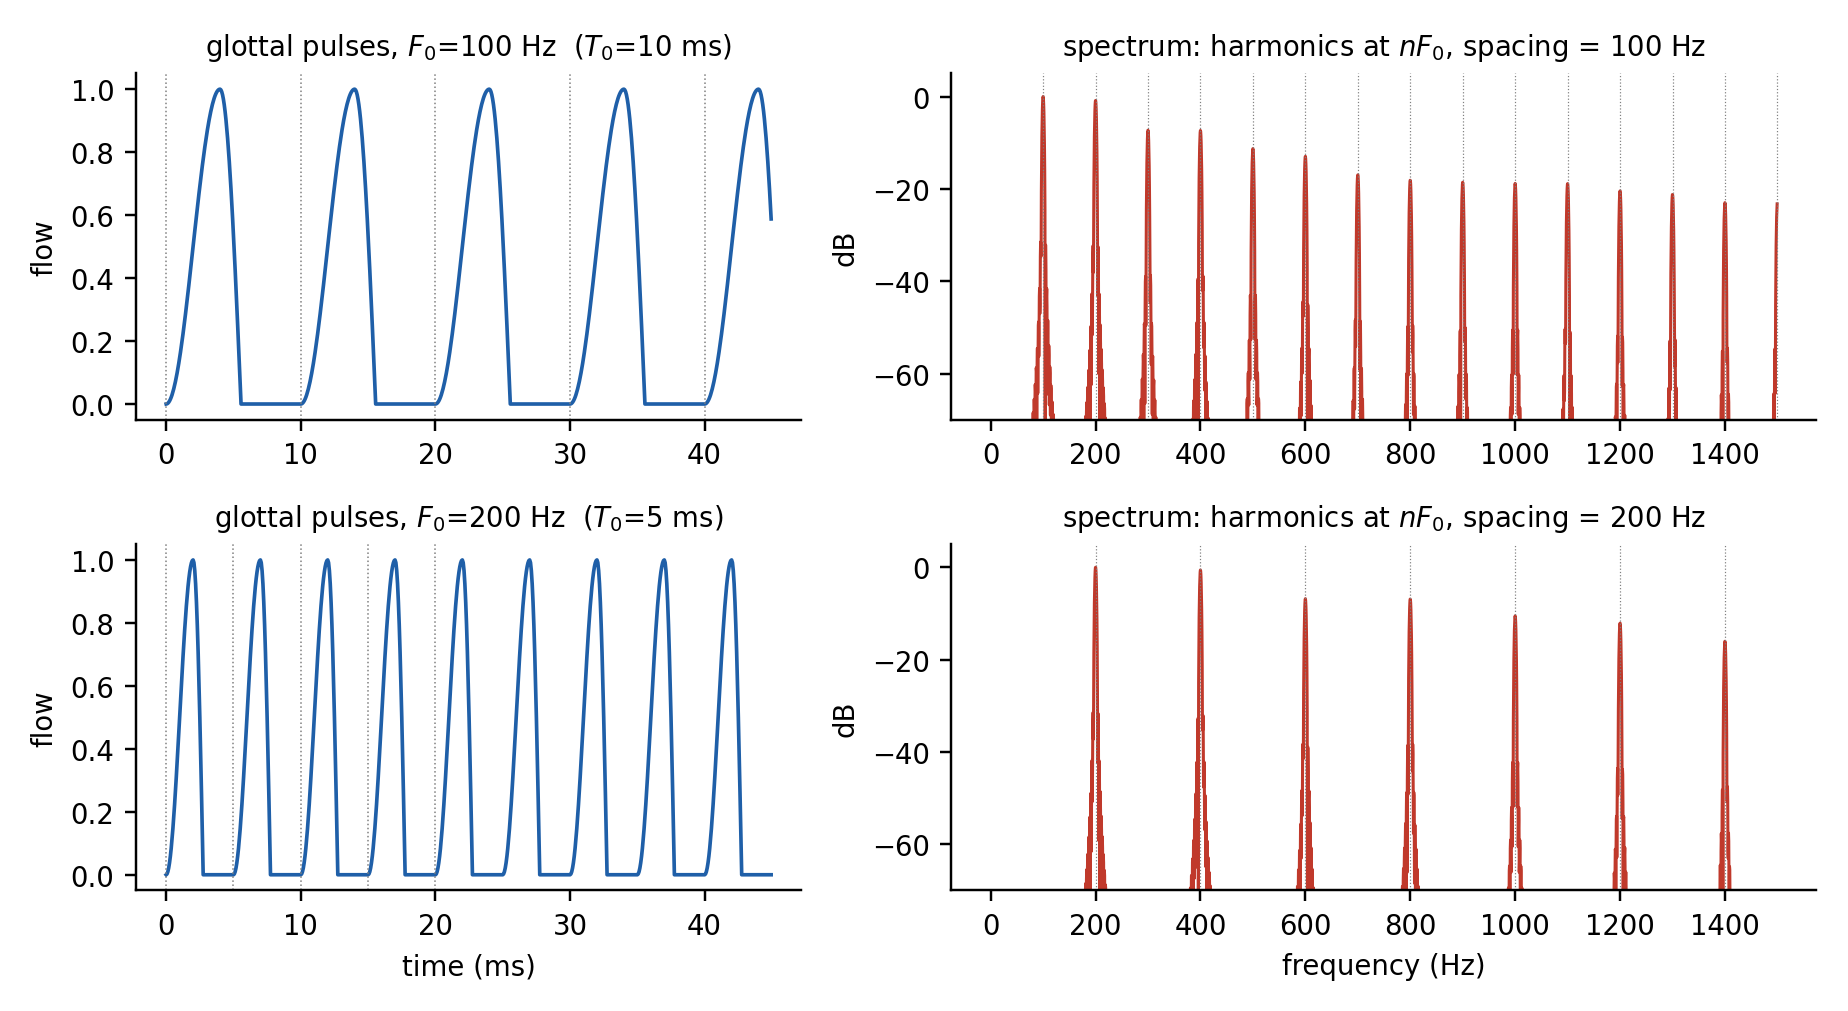
\includegraphics[width=0.95\textwidth]{../assets/figures/ch03-glottal-harmonics.png}
\caption{بالا: دنبالهٔ تپ‌های ساده‌شدهٔ هوای چاکنای با $F_0=100$ هرتز و طیف آن. پایین: همان با $F_0=200$ هرتز. هارمونیک‌ها در مضارب صحیح $F_0$ ظاهر می‌شوند و فاصلهٔ آن‌ها دقیقاً $F_0$ است (شکل افزوده).}
\end{figure}

فاصلهٔ دو هارمونیک متوالی برابر $F_0$ است؛ پس هرچه $F_0$ بزرگ‌تر (صدای زیرتر)، هارمونیک‌ها دورتر از هم‌اند و هرچه کوچک‌تر (صدای بم‌تر)، فشرده‌ترند. به همین دلیل از فاصلهٔ خطوط هارمونیکی در اسپکتروگرام می‌توان $F_0$ و تغییرات آن را خواند. اما $F_0$ و هارمونیک‌ها فقط «منبع» را توصیف می‌کنند و نمی‌گویند چرا «آ» با «ای» فرق دارد.

\section{اسپکتروگرام}

تبدیل فوریهٔ کل گفتار یک طیف واحد می‌دهد و زمان را از دست می‌دهد، در حالی که گفتار ایستا نیست. \term{اسپکتروگرام}{Spectrogram} تغییرات محتوای فرکانسی را در طول زمان نمایش می‌دهد. مراحل ساخت (\term{تبدیل فوریهٔ زمان-کوتاه}{Short-Time Fourier Transform, STFT}):
\begin{enumerate}
  \item سیگنال به پنجره‌ها یا فریم‌های کوتاه (مثلاً ۲۵ میلی‌ثانیه) بریده می‌شود (\eng{Windowing})؛ پنجره‌ها می‌توانند هم‌پوشانی (\eng{Overlap}) داشته باشند یا نداشته باشند؛
  \item روی هر فریم تبدیل فوریه اعمال و بزرگی طیف به دست می‌آید؛
  \item طیف‌ها به‌ترتیب زمان کنار هم چیده می‌شوند.
\end{enumerate}

محور افقی زمان، محور عمودی فرکانس و رنگ یا روشنایی هر نقطه، بزرگی (انرژی) آن مؤلفه در آن لحظه است. رنگ گرم یعنی بزرگی بالا، که معمولاً هارمونیک صدای ورودی است.

\boardfigure{0.7}{ch03-board-spectrogram-harmonics.png}{اسپکتروگرام یک صدای تقریباً پایدار: رنگ گرم یعنی بزرگی بالا (شباهت زیاد آن فرکانس با سیگنال ورودی، معمولاً هارمونیک)، رنگ سرد یعنی بزرگی پایین. خطوط افقی پررنگ هارمونیک‌ها هستند.}

\begin{correctionbox}{مقیاس رنگ معمولاً دسی‌بل است}
رنگ معمولاً لگاریتم بزرگی ($20\log_{10}|X|$) را نشان می‌دهد، نه خود بزرگی؛ و فاز کنار گذاشته می‌شود.
\end{correctionbox}

\begin{warningbox}{فرکانس و دامنه دو چیز متفاوت‌اند}
فرکانس یعنی سرعت نوسان و دامنه یعنی اندازهٔ نوسان. قرار داشتن یک مؤلفه در فرکانس بالاتر به معنی دامنهٔ بیشتر نیست. این تمایز در کلاس چند بار تأکید شد: در اسپکتروگرام «ارتفاع» فرکانس است و «پررنگی» دامنه.
\end{warningbox}

\section{مدل منبع--فیلتر}

وقتی فردی از «آ» به «ای» می‌رود و $F_0$ را ثابت نگه می‌دارد، صدا فرق می‌کند؛ این تغییر از $F_0$ نمی‌آید. پس مدل کامل‌تری لازم است.

\begin{definitionbox}{مدل منبع--فیلتر (\lr{Source--Filter})}
تولید گفتار به دو بخش (در تقریب مدل، مستقل) تقسیم می‌شود:
\begin{itemize}
  \item \textbf{منبع (\lr{Source}):} برای صداهای واک‌دار، ارتعاش تارهای صوتی که موجی دوره‌ای با $F_0$ و هارمونیک‌هایش تولید می‌کند؛
  \item \textbf{فیلتر (\lr{Filter}):} مجرای صوتی (\eng{Vocal Tract}) که بسته به شکلش بخش‌هایی از طیف را تقویت (تشدید) و بخش‌هایی را تضعیف می‌کند.
\end{itemize}
\end{definitionbox}

در حوزهٔ فرکانس، خروجی حاصل‌ضرب طیف منبع در پاسخ فرکانسی فیلتر است (در حوزهٔ زمان، کانولوشن؛ و در مقیاس لگاریتمی، جمع):
\[
\text{\lr{Output}}(f)=\text{\lr{Source}}(f)\times\text{\lr{Filter}}(f).
\]

\begin{figure}[htbp]
\centering
\begin{tikzpicture}[rtl, node distance=1.2cm, every node/.style={font=\small},
  box/.style={draw, rounded corners, minimum width=2.8cm, minimum height=1.1cm, align=center},
  arr/.style={-{Stealth[length=2.5mm]}, thick}]
  \node[box, fill=blue!10] (src) {منبع\\ \lr{Source}\\ \footnotesize تارهای صوتی};
  \node[box, left=of src, fill=green!10] (fil) {فیلتر\\ \lr{Filter}\\ \footnotesize مجرای صوتی};
  \node[box, left=of fil, fill=orange!12] (out) {خروجی\\ \lr{Output}\\ \footnotesize موج گفتار};
  \draw[arr] (src) -- (fil); \draw[arr] (fil) -- (out);
  \node[below=0.5mm of src, font=\scriptsize, align=center] {\lr{$F_0$ and harmonics}};
  \node[below=0.5mm of fil, font=\scriptsize, align=center] {\lr{formants $F_1,F_2,F_3$}};
  \node[below=0.5mm of out, font=\scriptsize, align=center] {\lr{harmonics shaped by formants}};
\end{tikzpicture}
\caption{نمای ساده‌شدهٔ مدل منبع--فیلتر برای صداهای واک‌دار (شکل افزوده).}
\end{figure}

استاد مجرا را شبیه یک لوله در نظر گرفتند: هر تغییر در موقعیت زبان، باز بودن دهان، فک، لب‌ها و محل تنگ‌شدگی، مشخصات فیلتر را عوض می‌کند. این همان پیوند مطلوب ماست: تغییر وضعیت اندام‌ها $\leftarrow$ تغییر قابل مشاهده در طیف موج.

\begin{figure}[htbp]
\centering
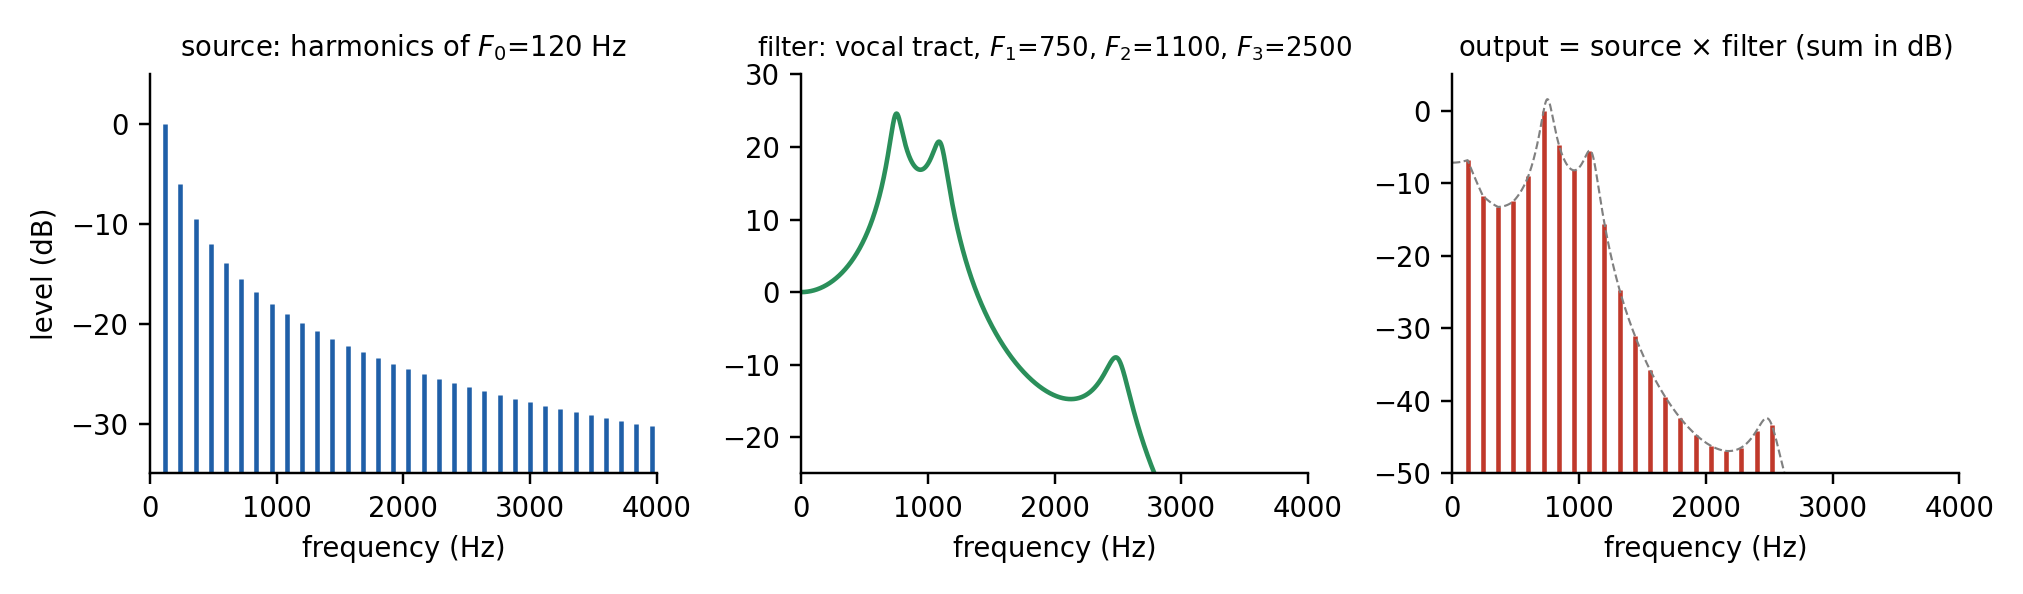
\includegraphics[width=0.95\textwidth]{../assets/figures/ch03-source-filter-spectra.png}
\caption{نمونهٔ عددی با $F_0=120$ هرتز: (الف) هارمونیک‌های منبع؛ (ب) پاسخ فرکانسی مجرا با فرمنت‌های $F_1=750$، $F_2=1100$ و $F_3=2500$ هرتز؛ (ج) خروجی (جمع دو منحنی در مقیاس دسی‌بل). خط‌چین پوش طیفی است (شکل افزوده).}
\end{figure}

\begin{correctionbox}{استقلال منبع و فیلتر تقریبی است}
مدل فرض می‌کند تغییر $F_0$ فرمنت‌ها را جابه‌جا نمی‌کند و برعکس؛ این تقریب برای بیشتر تحلیل‌ها خوب است، ولی برهم‌کنش منبع و مجرا و تابش از لب‌ها را نادیده می‌گیرد.
\end{correctionbox}

\textbf{آیا همهٔ صداها از تارهای صوتی می‌آیند؟} خیر؛ همخوان‌های بی‌واک مانند «س» منبعی از نویز آشفتگی جریان هوا دارند و هارمونیک ندارند. مدل «منبع = ارتعاش تارها» فقط برای صداهای واک‌دار است و تمرکز این جلسه بر همین حالت بود.

\section{فرمنت‌ها}

\begin{definitionbox}{فرمنت (\lr{Formant})}
فرمنت‌ها نواحی تشدید مجرای صوتی‌اند؛ نواحی فرکانسی که فیلتر آن‌ها را تقویت می‌کند. در طیف، قله‌ای پهن در پوش طیف و در اسپکتروگرام، نواری پررنگ‌اند. فرمنت‌ها بر اساس ترتیب فرکانسی نام‌گذاری می‌شوند: $F_1<F_2<F_3<\cdots$ (نه ترتیب زمانی).
\end{definitionbox}

فرمنت یک هارمونیک منفرد نیست؛ یک \emph{ناحیه} است که دامنهٔ چند هارمونیک مجاور را بالا می‌برد. فرمنت‌ها متعلق به فیلترند و ما هنگام تحلیل آن‌ها را \emph{نمی‌سازیم}، بلکه از سیگنال شناسایی می‌کنیم.

\textbf{ارتباط با نقشهٔ واکه‌ها} (مهم‌ترین ارتباط جلسه):
\begin{center}
\begin{tabular}{ll}
\toprule
ویژگی تولیدی & ویژگی آکوستیکی \\
\midrule
ارتفاع زبان / میزان بازشدگی دهان & $F_1$ \\
جلو یا عقب بودن زبان & $F_2$ \\
\bottomrule
\end{tabular}
\end{center}
\begin{itemize}
  \item $F_1$ برای واکه‌های بازتر بالاتر است: «آ» $F_1$ بالاتری از «ای» دارد.
  \item $F_2$ برای واکه‌های جلویی بالاتر و برای عقبی پایین‌تر است.
\end{itemize}

\boardfigure{0.8}{ch03-board-formants-iau.png}{اسپکتروگرام سه واکهٔ \eng{/i/}، \eng{/a/} و \eng{/u/} با خطوط افقی موقعیت $F_1$ تا $F_3$. در \eng{/i/} فاصلهٔ $F_1$ و $F_2$ بسیار زیاد است؛ در \eng{/a/} فرمنت اول بالاتر است؛ در \eng{/u/} هر دو فرمنت اول و دوم پایین‌اند.}

\begin{addedbox}{مقادیر نوعی فرمنت (مردان بالغ، تقریبی)}
\begin{center}
\begin{tabular}{lccc}
\toprule
واکه & $F_1$ & $F_2$ & $F_3$ \\
\midrule
\eng{/i/} («ای») & $270$ & $2290$ & $3010$ \\
\eng{/a/} («آ») & $730$ & $1090$ & $2440$ \\
\eng{/u/} («او») & $300$ & $870$ & $2240$ \\
\bottomrule
\end{tabular}
\end{center}
میانگین‌های واکه‌های انگلیسی (پترسون و بارنی، ۱۹۵۲) برحسب هرتز؛ فقط برای نشان‌دادن الگو.
\end{addedbox}

\begin{figure}[htbp]
\centering
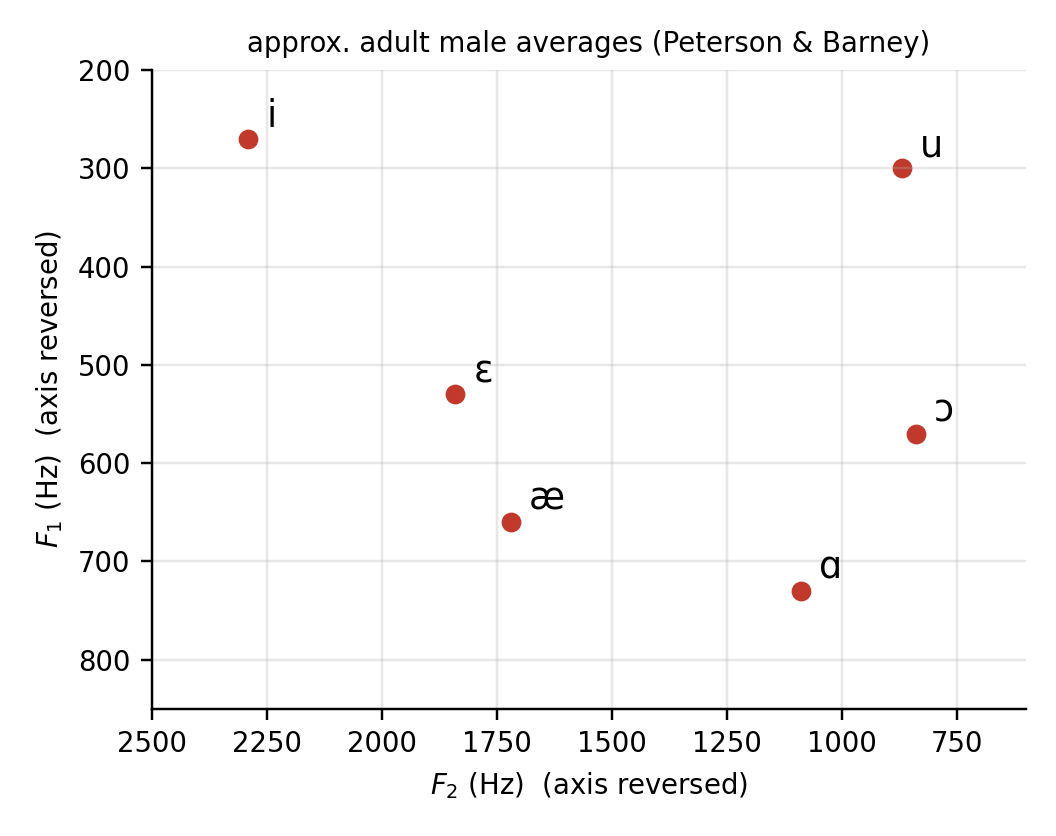
\includegraphics[width=0.55\textwidth]{../assets/figures/ch03-vowel-f1f2.png}
\caption{نقشهٔ آکوستیکی واکه‌ها در صفحهٔ $F_1$--$F_2$ (محورها معکوس)؛ شبیه نقشهٔ واکه‌ها در آواشناسی تولیدی (شکل افزوده).}
\end{figure}

\textbf{طول مجرا:} مجرای بلندتر، فرمنت‌ها را پایین‌تر می‌برد و مجرای کوتاه‌تر بالاتر (مجرای مردان معمولاً بلندتر است). این یکی از دلایلی است که $F_0$ به‌تنهایی جنسیت را مشخص نمی‌کند.

\begin{center}
\begin{tabular}{p{2.6cm}p{4.6cm}p{5.4cm}}
\toprule
ویژگی & هارمونیک & فرمنت \\
\midrule
منشأ اصلی & تناوب منبع (تارها) & تشدیدهای مجرای صوتی \\
نوع نمایش & مؤلفه در فرکانس مشخص & ناحیه یا قلهٔ تشدیدی در پوش طیف \\
ارتباط با $F_0$ & مضارب صحیح $F_0$ & لزوماً مضرب صحیح نیست \\
\bottomrule
\end{tabular}
\end{center}

\textbf{مثال کلاسی.} فرض کنید $F_0=120$ هرتز؛ هارمونیک‌ها $120,240,360,480,600,720,840,960,\dots$ هستند. اگر $F_1=750$ هرتز باشد، کدام هارمونیک‌ها بیشتر تقویت می‌شوند؟ پاسخ: ششم (۷۲۰) و هفتم (۸۴۰) که به ۷۵۰ نزدیک‌ترند (فاصله‌ها: $30$ و $90$ هرتز). میزان دقیق تقویت به شکل و پهنای قلهٔ تشدیدی بستگی دارد؛ به همین دلیل فرمنت در اسپکتروگرام یک ناحیهٔ پررنگ است، نه یک خط (شکل \ref{fig:ch03-harmonics-f1}).

\begin{figure}[htbp]
\centering
\begin{tikzpicture}[rtl, x=1cm,y=1cm,scale=1]
\def\u{0.0088}% cm per Hz
\fill[softblue] plot[smooth,domain=0:1340,samples=60] (\u*\x,{0.1+2.0*exp(-((\x-750)/230)^2)}) -- (\u*1340,0) -- (0,0) -- cycle;
\draw[mainblue, thick, smooth, domain=0:1340, samples=60, variable=\x] plot (\u*\x,{0.1+2.0*exp(-((\x-750)/230)^2)});
\foreach \n in {1,...,11}{
  \pgfmathtruncatemacro{\f}{120*\n}
  \pgfmathsetmacro{\h}{0.1+2.0*exp(-((\f-750)/230)^2)}
  \ifnum\n=6 \def\c{red!75!black}\def\w{1.8pt}\else\ifnum\n=7 \def\c{red!75!black}\def\w{1.8pt}\else\def\c{black!65}\def\w{0.9pt}\fi\fi
  \draw[\c, line width=\w] (\u*\f,0) -- (\u*\f,\h);
  \node[font=\scriptsize, below=1pt] at (\u*\f,0) {\lr{\n}};
  \node[font=\scriptsize, below=11pt, text=black!70] at (\u*\f,0) {\lr{\f}};
}
\draw[-{Stealth[length=2mm]}, thick] (0,0) -- (\u*1400,0) node[right, font=\small] {\lr{Hz}};
\draw[dashed, red!75!black] (\u*750,0) -- (\u*750,2.65);
\node[above, font=\small, red!75!black] at (\u*750,2.65) {\lr{$F_1=750$ Hz}};
\node[font=\scriptsize, anchor=east] at (-0.15,-0.2) {شماره};
\node[font=\scriptsize, anchor=east, text=black!70] at (-0.15,-0.62) {\lr{$nF_0$}};
\end{tikzpicture}
\caption{مثال تخته: با $F_0=120$ هرتز و $F_1=750$ هرتز، هارمونیک‌ها در ۱۲۰، ۲۴۰، ۳۶۰، \dots هرتز قرار دارند و شمارهٔ هرکدام زیر آن نوشته شده است. هارمونیک‌های نزدیک به قلهٔ تشدیدی (ششم و هفتم، ۷۲۰ و ۸۴۰ هرتز، با رنگ قرمز) بیشترین تقویت را می‌گیرند؛ منحنی آبی شکل کلی فیلتر مجرای صوتی است (منحنی افزوده) (بازسازی‌شده از تختهٔ کلاس).}
\label{fig:ch03-harmonics-f1}
\end{figure}

\section{اسپکتروگرام باند باریک و باند پهن}

کلید فهم این دو نوع، یک مبادله (\eng{trade-off}) بنیادی است: پنجرهٔ \textbf{کوتاه} تغییرات سریع زمانی را بهتر نشان می‌دهد ولی فرکانس‌های نزدیک را بد تفکیک می‌کند؛ پنجرهٔ \textbf{بلند} برعکس. وضوح فرکانسی تقریباً با معکوس طول پنجره متناسب است ($\Delta f\sim 1/L$؛ مثلاً با $f_s=16000$ و $N=512$ نمونه، $\Delta f=31.25$ هرتز).

\begin{definitionbox}{باند پهن در برابر باند باریک}
\textbf{باند پهن (\lr{Wideband}):} پنجرهٔ کوتاه (حدود ۳ تا ۵ میلی‌ثانیه؛ در کلاس ۵). وضوح زمانی بالا، وضوح فرکانسی پایین؛ هارمونیک‌ها در هم ادغام می‌شوند و پوش طیفی (فرمنت‌ها) دیده می‌شود.

\textbf{باند باریک (\lr{Narrowband}):} پنجرهٔ بلندتر (حدود ۲۰ تا ۵۰ میلی‌ثانیه؛ در کلاس ۳۰). وضوح فرکانسی بالا، وضوح زمانی پایین؛ هارمونیک‌ها به‌صورت خطوط افقی باریک و مجزا دیده می‌شوند.
\end{definitionbox}

\begin{center}
\begin{tabular}{lcc}
\toprule
ویژگی & باند پهن & باند باریک \\
\midrule
طول پنجره & کوتاه & بلند \\
وضوح زمانی & بالا & پایین \\
وضوح فرکانسی & پایین & بالا \\
نمایش مناسب‌تر & فرمنت‌ها & هارمونیک‌ها \\
\bottomrule
\end{tabular}
\end{center}

\begin{exambox}{نکتهٔ مهم استاد}
این دو نوع اسپکتروگرام مربوط به دو سیگنال متفاوت نیستند؛ هر دو از \emph{یک} سیگنال با تنظیم متفاوت پنجره ساخته می‌شوند. دقت زمانی و فرمنت $\Leftarrow$ \eng{wideband}؛ دقت فرکانسی و هارمونیک‌ها $\Leftarrow$ \eng{narrowband}.
\end{exambox}

فرمنت‌ها با حرکت سریع زبان و دهان تغییر می‌کنند و ردگیری آن‌ها وضوح زمانی خوب می‌خواهد؛ به همین دلیل باند پهن برای فرمنت‌ها مناسب‌تر است.

\begin{figure}[htbp]
\centering
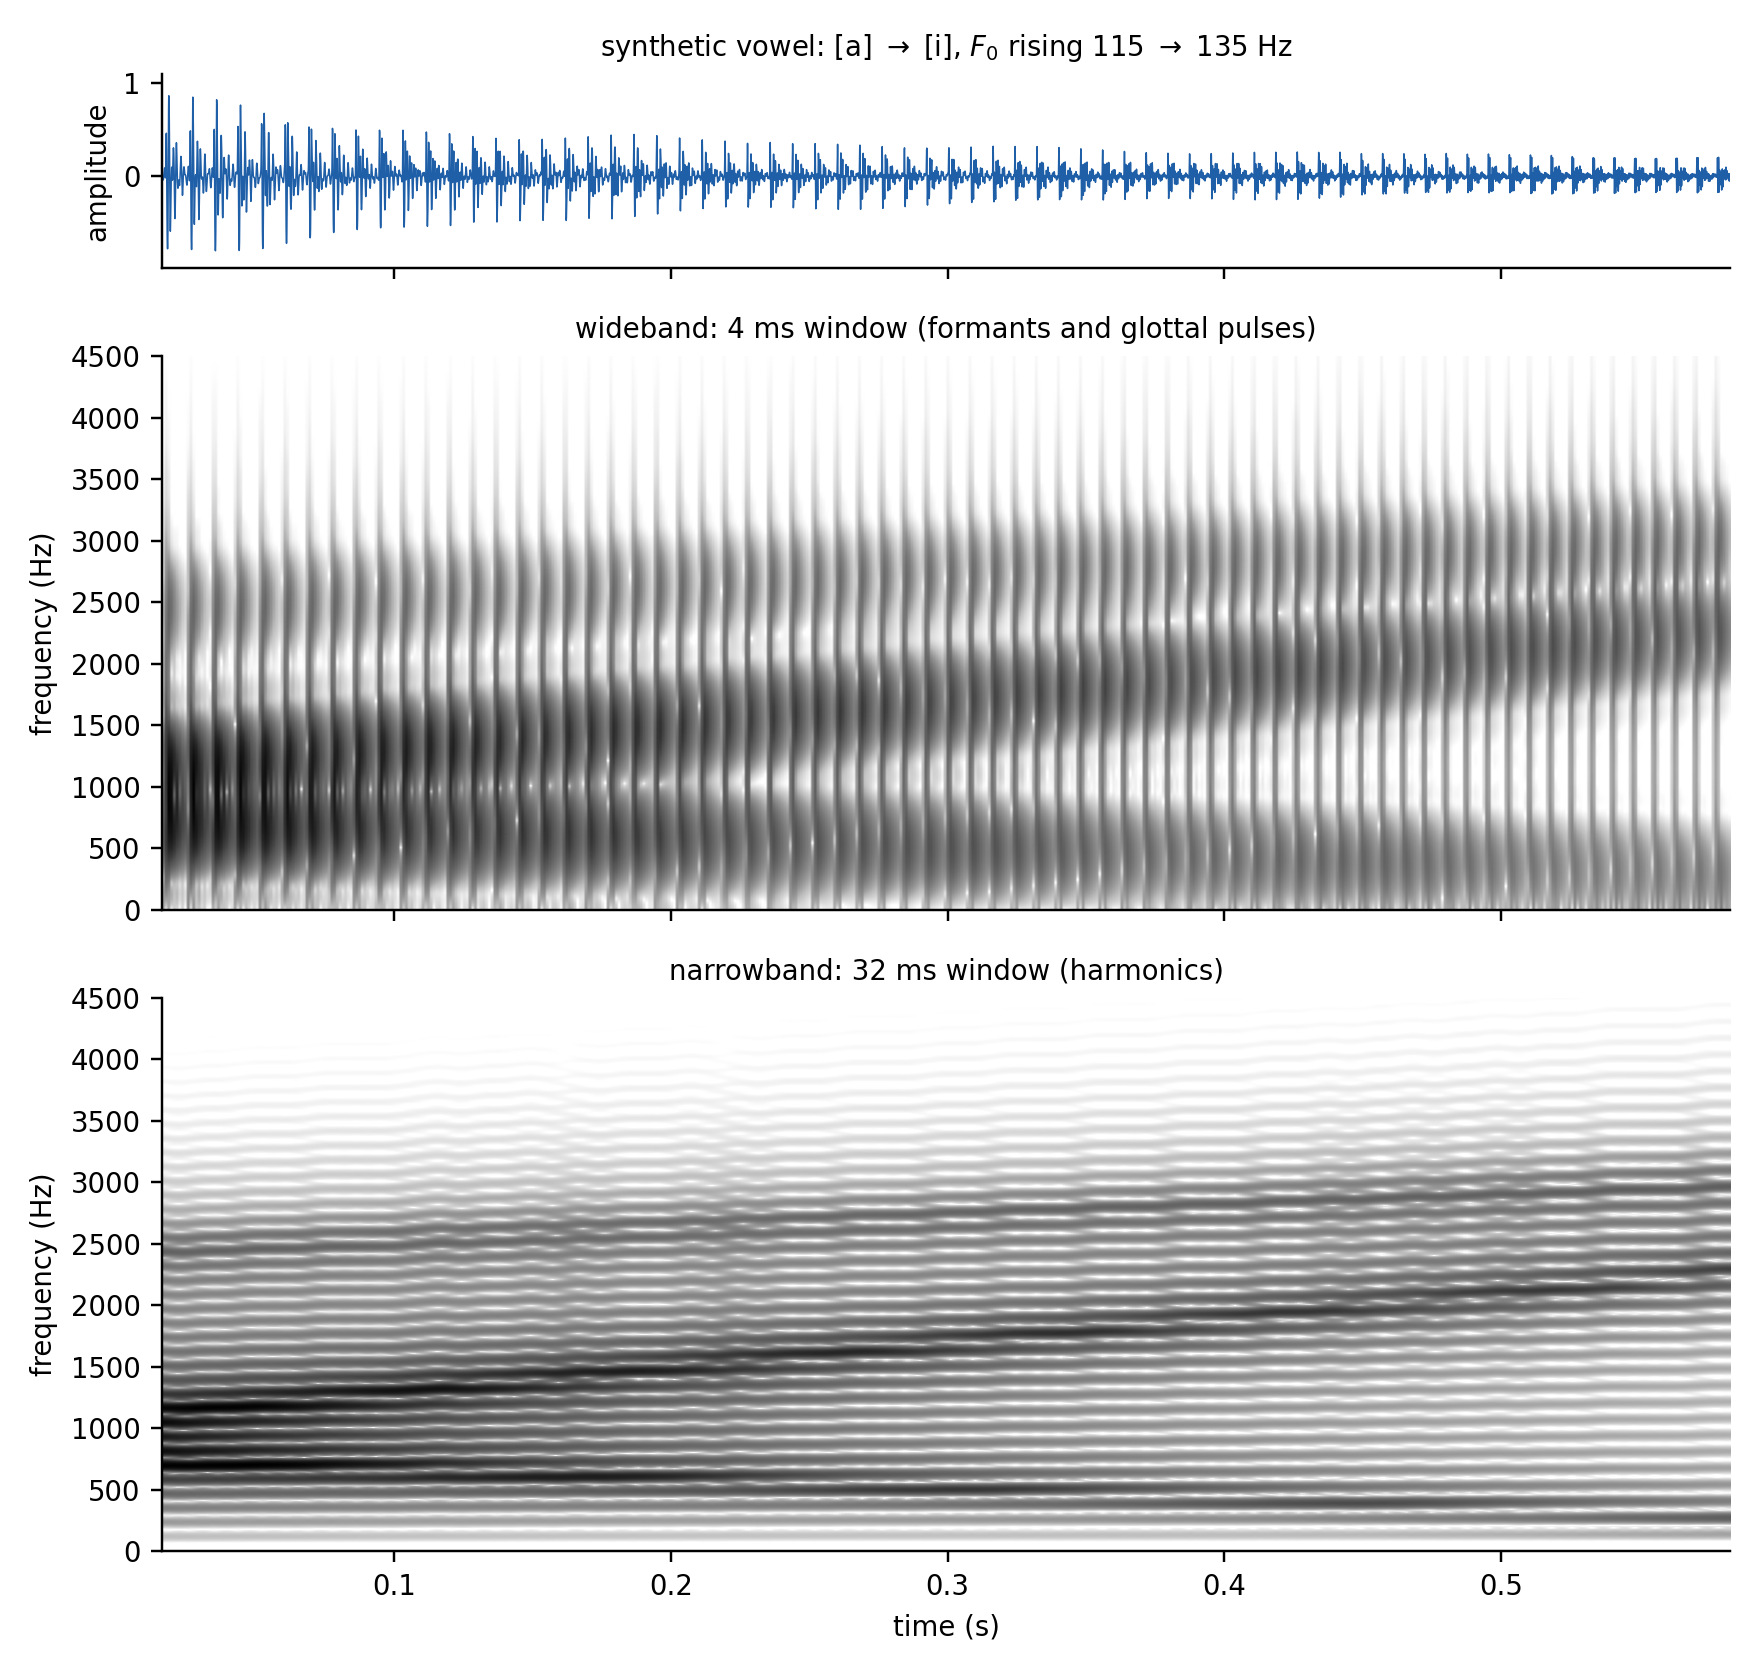
\includegraphics[width=0.95\textwidth]{../assets/figures/ch03-wideband-narrowband.png}
\caption{اسپکتروگرام باند پهن (پنجرهٔ ۴ میلی‌ثانیه) و باند باریک (۳۲ میلی‌ثانیه) از \emph{یک} واکهٔ ترکیبی که از «آ» به «ای» می‌رود. باند پهن نوارهای فرمنتی و خطوط عمودی تپ‌های چاکنایی را نشان می‌دهد؛ باند باریک خطوط افقی هارمونیک‌ها را (شکل افزوده).}
\end{figure}

\section{پرسش و پاسخ}

\begin{itemize}
  \item \textbf{آیا هارمونیک‌ها و فرمنت‌ها را می‌توان کاملاً جدا کرد؟} خیر؛ فیلتر روی طیف منبع اثر گذاشته و هر دو در سیگنال حضورند. با تغییر نوع اسپکتروگرام فقط یکی بهتر دیده می‌شود.
  \item \textbf{اگر دهان ثابت بماند، فرمنت‌ها حذف می‌شوند؟} خیر؛ فیلتر همچنان هست و فرمنت‌ها نوارهای افقی نسبتاً ثابت‌اند.
  \item \textbf{آیا با تغییر فرمنت‌ها \eng{Pitch} از بین می‌رود؟} خیر؛ فیلتر بر دامنهٔ هارمونیک‌ها اثر می‌گذارد، نه بر $F_0$.
  \item \textbf{آیا فرمنت‌ها را می‌توان عددی استخراج کرد؟} بله، به‌عنوان ویژگی عددی؛ الگوریتم‌هایش در این جلسه بررسی نشد.
\end{itemize}

\section{کاربردهای اسپکتروگرام و تمرین}

{\emergencystretch=3em اسپکتروگرام ابزاری آموزشی نیست و در مسائل واقعی مانند \term{تشخیص احساس از گفتار}{Speech Emotion Recognition} به کار می‌رود. در بخش عملی، استاد ابزاری پایتونی (مبتنی بر پردازش سیگنال، با کاربرد در گفتاردرمانی) را روی کلمهٔ «سیب» نشان دادند: در نمایش اول خطوط هارمونیکی واضح‌تر بودند و برای دیدن بهتر فرمنت‌ها باید اندازهٔ پنجره را کوتاه کرد (باند پهن).\par}

\begin{assignmentbox}{تمرین اول: اسپکتروگرام}
تمرین اول با اسپکتروگرام مرتبط است؛ جزئیات اجرایی در این جلسه بیان نشد. مفاهیم لازم: شکل موج، $F_0$ و هارمونیک‌ها، تبدیل فوریه و پنجره‌بندی، تولید و تحلیل اسپکتروگرام، تفاوت باند پهن و باریک، و مشاهده و تفسیر فرمنت‌ها.
\end{assignmentbox}

\section{جمع‌بندی}

\begin{center}
\begin{tabular}{p{3.4cm}p{9.4cm}}
\toprule
مفهوم & تعریف و نقش \\
\midrule
فرکانس پایه $F_0$ & $1/T_0$؛ مرتبط با \eng{Pitch}؛ وابسته به طول، جرم و کشش تارها \\
هارمونیک‌ها & مضارب صحیح $F_0$، با فاصلهٔ $F_0$ \\
اسپکتروگرام & بزرگی \eng{STFT}؛ محتوای فرکانسی در طول زمان \\
منبع / فیلتر & تارهای صوتی (واک‌دار) / مجرای صوتی که طیف منبع را شکل می‌دهد \\
فرمنت‌ها & نواحی تشدید مجرا ($F_1<F_2<F_3$)؛ $F_1$: ارتفاع/بازشدگی، $F_2$: جلو--عقب \\
باند پهن / باریک & پنجرهٔ کوتاه، فرمنت‌ها / پنجرهٔ بلند، هارمونیک‌ها \\
\bottomrule
\end{tabular}
\end{center}

رابطه با جلسهٔ قبل: آواشناسی تولیدی وضعیت اندام‌ها را توصیف می‌کند؛ مدل منبع--فیلتر آن را به تحریک تارها و فیلتر مجرا ترجمه می‌کند؛ $F_0$، هارمونیک‌ها و فرمنت‌ها آثار قابل‌اندازه‌گیری آن هستند و اسپکتروگرام ابزار مشاهدهٔ آن‌ها است.

\begin{exambox}{نکات مهم برای مرور و امتحان}
\begin{itemize}
  \item نمره: ۱۰ عملی (گزارش یا ارائه) + ۱۰ نظری (میان‌ترم و پایان‌ترم)؛ تمرین اول دربارهٔ اسپکتروگرام است.
  \item $F_0$ ویژگی فیزیکی و \eng{Pitch} ادراکی است؛ $F_0$ بالاتر یعنی صدای زیرتر. $F_0$ به‌تنهایی جنسیت را تعیین نمی‌کند؛ طول مجرا نیز مؤثر است.
  \item هارمونیک‌ها در $nF_0$ و با فاصلهٔ $F_0$ هستند؛ $F_0$ بزرگ‌تر یعنی هارمونیک‌های دورتر.
  \item اسپکتروگرام = پنجره‌بندی + فوریه برای هر پنجره + کنار هم چیدن (افقی زمان، عمودی فرکانس، رنگ بزرگی). فرکانس و دامنه متفاوت‌اند.
  \item $\text{Output}(f)=\text{Source}(f)\times\text{Filter}(f)$؛ منبع = تارها (واک‌دار)، فیلتر = مجرا.
  \item فرمنت ناحیهٔ تشدیدی مجراست، نه یک هارمونیک؛ $F_1$ با ارتفاع/بازشدگی و $F_2$ با جلو/عقب بودن زبان مرتبط است؛ مجرای بلندتر، فرمنت‌های پایین‌تر. فرمنت‌ها «شناسایی» می‌شوند، نه «ساخته».
  \item باند پهن (پنجرهٔ حدود ۵ میلی‌ثانیه) $\leftarrow$ فرمنت‌ها و وضوح زمانی؛ باند باریک (حدود ۳۰ میلی‌ثانیه) $\leftarrow$ هارمونیک‌ها و وضوح فرکانسی؛ هر دو از یک سیگنال‌اند.
  \item مثال کلاسی: $F_0=120$ و $F_1=750$ هرتز $\Leftarrow$ هارمونیک‌های ششم (۷۲۰) و هفتم (۸۴۰) بیشتر تقویت می‌شوند.
\end{itemize}
\end{exambox}

\chapter{فرمنت‌ها، نرم‌افزار \eng{Praat} و فضای واکه‌ای}

هدف این جلسه آن است که از روی سیگنال صوتی، ویژگی‌های \term{آکوستیکی}{Acoustic} مانند \eng{F1} و \eng{F2} را اندازه بگیریم و آن‌ها را به ویژگی‌های \term{تولیدی}{Articulatory} مانند ارتفاع و جلو یا عقب‌بودن زبان نگاشت کنیم. ابزار عملی این کار نرم‌افزار \eng{Praat} و نتیجهٔ کار، \term{فضای واکه‌ای}{Vowel Space} است که در گفتاردرمانی، تشخیص صدای جعلی و پایش بیماری‌های عصبی به کار می‌رود.

\section{مرور کوتاه: از فرکانس پایه تا فرمنت}
جزئیات فوریه، هارمونیک‌ها و مدل منبع–فیلتر در فصل ۳ آمده است. نکته‌های مرور شده در ابتدای جلسه:

\begin{itemize}
  \item \textbf{فرکانس پایه:} اگر موجی در هر $T$ ثانیه یک دورهٔ کامل بزند، $f_0=1/T$ است. برای \eng{Pitch} تکرار قله‌های اصلی، یعنی کندترین الگوی تناوبی، را در نظر می‌گیریم. $f_0$ به \emph{منبع} (چین‌های صوتی) و فرمنت‌ها به \emph{فیلتر} (مجرای صوتی) مربوط‌اند.
  \item \textbf{\eng{Magnitude} در برابر دامنه:} ضریب فوریه عدد مختلط $X=a+jb$ است؛ اندازهٔ آن $|X|=\sqrt{a^2+b^2}$ سهم آن فرکانس در سیگنال است و زاویهٔ آن فاز. دامنهٔ زمانی سیگنال و \eng{Magnitude} طیفی یکی نیستند. در اسپکتروگرام رنگ گرم‌تر یعنی مقدار طیفی بیشتر.
  \item \textbf{تعامد:} موج‌های مبنا باید متعامد باشند تا هر کدام مؤلفه‌ای مستقل را بسنجند: ضرب داخلی دو موج صفر باشد ($\int_0^T x_1(t)x_2(t)\,dt=0$). موج‌هایی با تعداد صحیح دوره در بازهٔ $T$ (فرکانس‌های $1/T,2/T,\dots$) چنین مجموعه‌ای می‌سازند.
  \item \textbf{هارمونیک‌ها:} فرکانس‌ها $f_n=nf_0$ هستند ولی ضریب برخی می‌تواند صفر باشد؛ مثلاً موج مربعی با چرخهٔ کاری ۵۰ درصد فقط هارمونیک‌های فرد دارد.
\end{itemize}

\begin{exambox}{پرسش و پاسخ: آیا تعداد هارمونیک‌ها بی‌نهایت است؟}
از نظر ریاضی بله، اما در عمل نرخ نمونه‌برداری (نایکویست) و هدف تحلیل آن را محدود می‌کند و فقط بخش مفید طیف بررسی می‌شود.
\end{exambox}

\subsection{هارمونیک در برابر فرمنت}
هارمونیک‌ها ویژگی \emph{سیگنال تناوبی} (منبع) هستند، در حالی که \term{فرمنت‌ها}{Formants} نواحی تشدید \emph{مجرای صوتی} (فیلتر) را توصیف می‌کنند و به صورت برآمدگی‌های پوش طیفی دیده می‌شوند. با نگاه به هارمونیک‌ها نمی‌توان فهمید زبان کجاست؛ برای این کار باید فرمنت‌ها را استخراج کرد. یکی از روش‌های رایج تخمین فرمنت \term{کدگذاری پیش‌بینی خطی}{Linear Predictive Coding (LPC)} است.

\begin{table}[htbp]
\centering
\caption{مقایسهٔ اسپکتروگرام پهن‌باند و باریک‌باند}
\begin{tabular}{p{3.2cm}p{5.2cm}p{5.2cm}}
\toprule
ویژگی & \eng{Wideband} & \eng{Narrowband} \\
\midrule
طول پنجره & کوتاه‌تر (حدود ۵ میلی‌ثانیه) & بلندتر \\
تفکیک زمانی / فرکانسی & زمانی بیشتر، فرکانسی کمتر & زمانی کمتر، فرکانسی بیشتر \\
ظاهر طیف & نواحی پهن انرژی؛ فرمنت‌ها دیده می‌شوند & خطوط هارمونیکی جداگانه \\
کاربرد & دنبال‌کردن فرمنت‌ها و حرکت اندام‌ها & بررسی هارمونیک‌ها و $f_0$ \\
\bottomrule
\end{tabular}
\end{table}

چون زبان و سایر اندام‌ها سریع جابه‌جا می‌شوند، برای دیدن فرمنت‌ها از نمای پهن‌باند استفاده می‌کنیم.

\section{نگاشت ویژگی‌های آکوستیکی به ویژگی‌های تولیدی}
در پردازش گفتار معمولاً موقعیت واقعی زبان را مستقیم اندازه نمی‌گیریم؛ در عوض ویژگی‌های آکوستیکی را از صوت استخراج و برای توصیف فضای واکه‌ای به کار می‌بریم. دو فرمنت اول بیشترین نقش را دارند.

\begin{definitionbox}{نگاشت \eng{F1} و \eng{F2} به ویژگی‌های تولیدی}
\begin{itemize}
  \item \term{فرمنت اول}{F1}: رابطهٔ \emph{معکوس} با ارتفاع زبان. زبان بالاتر (واکهٔ بسته) $\Leftarrow$ \eng{F1} کمتر؛ زبان پایین‌تر (واکهٔ باز) $\Leftarrow$ \eng{F1} بیشتر.
  \item \term{فرمنت دوم}{F2}: مرتبط با جلو یا عقب بودن زبان. زبان جلوتر $\Leftarrow$ \eng{F2} بیشتر؛ زبان عقب‌تر $\Leftarrow$ \eng{F2} کمتر.
  \item \term{گرد شدن لب}{Lip Rounding}: \eng{F2} را کاهش می‌دهد.
\end{itemize}
\end{definitionbox}

\begin{correctionbox}{این رابطه‌ها تقریبی‌اند}
فرمنت‌ها تشدیدهای کل مجرای صوتی‌اند، نه یک «حفرهٔ» مشخص؛ \eng{F1} علاوه بر ارتفاع زبان به باز بودن فک و تنگی حلق نیز حساس است. به همین دلیل واکهٔ عقبی گرد مانند \eng{/u/} هم \eng{F1} هم \eng{F2} پایین دارد. پاسخ استاد به پرسش «آیا قانون ثابت است؟»: این یک قاعدهٔ کلی آواشناختی است، نه رابطه‌ای بدون استثنا؛ برای یک گروه جدید رابطه را از پیش فرض نمی‌کنیم، مقادیر واقعی را اندازه می‌گیریم و تفاوت‌ها را تفسیر می‌کنیم.
\end{correctionbox}

\begin{addedbox}{مثال عددی: لولهٔ یکنواخت و اثر طول مجرا}
مجرای خنثی را می‌توان لولهٔ یک‌سر بسته (چین‌های صوتی) و یک‌سر باز (لب‌ها) گرفت: $F_n=\dfrac{(2n-1)\,c}{4L}$ با $c\approx 35000$ سانتی‌متر بر ثانیه. برای $L=17.5$ سانتی‌متر (مرد بزرگسال): $F_1=500$، $F_2=1500$ و $F_3=2500$ هرتز. برای $L=11$ سانتی‌متر (کودک): $F_1\approx 795$ و $F_2\approx 2386$ هرتز. پس مجرای کوتاه‌تر یعنی فرمنت بالاتر، و فضای واکه‌ای باید برای هر گروه جداگانه ساخته شود.
\end{addedbox}

\section{کار عملی با \eng{Praat}}
\eng{Praat} نرم‌افزار رایگان تحلیل و برچسب‌گذاری گفتار است (\eng{Boersma} و \eng{Weenink}، آمستردام). استاد آن را برای پل زدن میان ویژگی‌های آکوستیکی و تولیدی معرفی کرد؛ تمرکز بر دو کار بود: استخراج فرمنت‌ها و برچسب‌گذاری (\eng{Annotation}).

\subsection{تحلیل صوت و اندازه‌گیری فرمنت}
استاد چند واکه («ای»، «آ»، «او») را ضبط کرد. در محیط تحلیل، شکل موج در بالا، \term{طیف‌نگاره}{Spectrogram} در پس‌زمینه، منحنی آبی \eng{Pitch} و نقطه‌های قرمز \eng{Formants} دیده می‌شود. با کلیک روی هر لحظه، فرمنت‌ها همان لحظه نمایش داده می‌شوند (در کلاس: \eng{F1} حدود ۳۴۰، \eng{F2} حدود ۲۰۰۰ و \eng{F3} حدود ۳۰۰۰ هرتز، الگوی شبیه \eng{/i/}؛ واحد هرتز است). این‌ها اندازه‌گیری یک لحظه‌اند، نه مقدار ثابت واکه.

لازم نیست فقط در یک نقطه بخوانیم: بازهٔ زمانی یک واکه (مثلاً «آ») را انتخاب، میانگین \eng{F1} و \eng{F2} را از \eng{Praat} می‌گیریم و برای تحلیل ذخیره می‌کنیم. در پژوهش‌ها معمولاً فرمنت در میانهٔ واکه (حدود ۵۰ درصد مدت) یا میانگین ۲۰ تا ۸۰ درصد خوانده می‌شود تا اثر همخوان‌های مجاور کم شود.

\begin{correctionbox}{سقف فرمنت (\eng{Maximum formant}) را بر حسب گوینده تنظیم کنید}
\eng{Praat} فرمنت‌ها را با روش \eng{Burg} (نوعی \eng{LPC}) تخمین می‌زند. راهنمای معمول با ۵ فرمنت: حدود ۵۰۰۰ هرتز برای مردان، ۵۵۰۰ (پیش‌فرض) برای زنان و مقادیر بالاتر برای کودکان. سقف نامناسب فرمنتی را حذف یا اضافه می‌کند. خروجی را همیشه با طیف‌نگاره بازبینی کنید؛ وقتی $f_0$ بالا است (زنان و کودکان) ممکن است هارمونیک به جای فرمنت انتخاب شود. برای \eng{Pitch} نیز بازهٔ جست‌وجو را متناسب با گوینده بگذارید (مردان حدود ۷۵ تا ۳۰۰ و زنان ۱۰۰ تا ۵۰۰ هرتز) وگرنه $f_0$ نصف یا دو برابر می‌شود.
\end{correctionbox}

\subsection{برچسب‌گذاری گفتار با \eng{TextGrid}}
مهم‌ترین کاربرد \eng{Praat} در این جلسه \eng{Annotation} بود: مشخص‌کردن مرزهای زمانی و برچسب‌زدن بخش‌های صوت. ساختار آن \eng{TextGrid} است و از چند لایه (\eng{Tier}) ساخته می‌شود. استاد سه سطح را مثال زد:

\begin{center}
\begin{tabular}{lccc}
\toprule
لایه & \multicolumn{3}{c}{برچسب‌ها} \\
\midrule
\eng{Word Tier} (سطح واژه) & \multicolumn{3}{c}{ای آ او} \\
\eng{Syllable Tier} (سطح هجا) & ای & آ & او \\
\eng{Phoneme Tier} (سطح واج) & \eng{/i/} & \eng{/ɑ/} & \eng{/u/} \\
\bottomrule
\end{tabular}
\end{center}

با تعیین بازهٔ هر واکه یا همخوان، علاوه بر برچسب زبانی، اطلاعات آکوستیکی همان بازه هم استخراج می‌شود. نتیجه مجموعه‌داده‌ای است که برای هر بازه می‌گوید چه واجی تولید شده، \eng{F1} و \eng{F2} آن چقدر بوده و گوینده به کدام گروه آماری تعلق دارد.

\boardfigure{0.8}{ch04-praat-textgrid.png}{نمونهٔ یک \eng{TextGrid} در \eng{Praat}: شکل موج، طیف‌نگاره و سه لایهٔ برچسب برای یک جملهٔ پیکرهٔ \eng{AusKidTalk}.}

\section{ساخت پیکرهٔ گفتاری برای یک جامعهٔ آماری خاص}
استاد دستیار صوتی کودکان را مثال زد: سامانهٔ تشخیص گفتاری که برای بزرگسالان خوب کار می‌کند، روی گفتار کودکان بیشتر خطا می‌کند (مجرای کوتاه‌تر و فرمنت‌های بالاتر). راه‌حل ساخت پیکرهٔ اختصاصی است:
\begin{enumerate}
  \item ضبط نمونه‌های صوتی از کودکان جامعهٔ هدف؛
  \item بررسی در \eng{Praat} و تعیین مرز واژه‌ها و واج‌ها؛
  \item برچسب‌زدن واکه‌ها و استخراج \eng{F1} و \eng{F2}؛
  \item به‌دست‌آوردن دامنهٔ آماری هر واکه در آن گروه.
\end{enumerate}
خروجی جدولی است با ستون‌های «واکه»، «دامنهٔ \eng{F1}» و «دامنهٔ \eng{F2}» که مقادیرش باید از داده‌های واقعی بیاید و جداگانه برای زنان، مردان، کودکان یا گروه‌های خاص تهیه می‌شود.

\subsection{چارچوب \eng{ASR} + بازبینی انسانی}
مقالهٔ \eng{AusKidTalk} (\eng{LREC 2026}) رونویسی گفتار پیوستهٔ کودکان استرالیایی را شرح می‌دهد: متن اولیه با \eng{ASR} (نرخ خطای واژه ۲۳ درصد) تولید و سپس به‌دست انسان اصلاح شد؛ اصلاح دستی حدود ۱۱ برابر مدت گفتار زمان برد، در حالی که رونویسی دستی کامل با راستی‌آزمایی حدود ۵۰ برابر است. فرایند کلاس:
\begin{enumerate}
  \item ضبط گفتار کودکان؛
  \item تولید متن اولیه با مدل \eng{ASR} مانند \eng{Whisper}؛
  \item آماده‌سازی \eng{TextGrid} و هم‌زمان‌سازی متن با صوت؛
  \item بازبینی انسانی (\eng{Annotator}): گوش‌دادن و اصلاح برچسب‌ها و مرزها؛
  \item ساخت پیکرهٔ نهایی.
\end{enumerate}
کار برچسب‌زن از نوشتن از صفر به «بازبینی و تصحیح» تبدیل می‌شود که سریع‌تر و عملی‌تر است. پیکرهٔ اصلاح‌شده را می‌توان برای \term{تنظیم دقیق}{Fine-tuning} مدلی مانند \eng{Whisper} به کار برد؛ استاد این را با ایدهٔ استفاده از داده‌های دشوار (خطاهای مدل قبلی) مرتبط دانست.

\begin{definitionbox}{نرخ خطای واژه (\eng{WER})}
\[
\text{\lr{WER}}=\frac{S+D+I}{N}
\]
$S$ جانشینی، $D$ حذف، $I$ درج و $N$ تعداد واژه‌های مرجع است. مثال: مرجع با $N=10$ واژه، یک واژه تغییر کرده ($S=1$) و یکی حذف شده ($D=1$): $\text{\lr{WER}}=2/10=20\%$. چون درج‌ها هم شمرده می‌شوند، \eng{WER} می‌تواند از ۱۰۰ درصد بیشتر شود.
\end{definitionbox}

\begin{exambox}{نکتهٔ پژوهشی: مستندسازی برچسب‌گذاری}
استاد گفت هنگام انتشار پژوهش، روش برچسب‌گذاری باید کاملاً مستند شود: چه کسانی برچسب زده‌اند، تجربه و تحصیلاتشان، ابزار و روش، نحوهٔ اصلاح خطاهای خروجی خودکار و سنجش کیفیت نهایی. این‌ها برای اعتبار و بازتولیدپذیری لازم‌اند.
\end{exambox}

\section{فضای واکه‌ای}
\subsection{تعریف و نمودار \eng{F1–F2}}
\begin{definitionbox}{فضای واکه‌ای (\eng{Vowel Space})}
نمایش هندسی جایگاه واکه‌ها بر پایهٔ ویژگی‌های تولیدی (ارتفاع و جلو یا عقب بودن زبان) یا آکوستیکی. در نمایش آکوستیکی هر واکه نقطه‌ای است با مختصات $V=(F_1,F_2)$ و با گردآوری نمونه‌های متعدد، پراکندگی و دامنهٔ هر واکه دیده می‌شود.
\end{definitionbox}

روی تخته دو نقشه مقایسه شد: «نقشهٔ استاندارد و تئوریک الفبای بین‌المللی آواشناسی» که صرفاً توصیفی است، و «نقشهٔ اندازه‌گیری‌شده بر اساس داده‌های آکوستیک \eng{Praat}»؛ هدف درس رسیدن به نقشهٔ دوم است. شکل~\ref{fig:ch04-vowel-ellipses} نسخهٔ اندازه‌گیری‌شدهٔ واکه‌های انگلیسی را نشان می‌دهد.

\boardfigure{0.5}{ch04-english-vowel-ellipses.png}{نقشهٔ اندازه‌گیری‌شدهٔ واکه‌های انگلیسی؛ هر بیضی پراکندگی یک واکه در \eng{F1–F2} است. محورها معکوس رسم شده‌اند تا با نقشهٔ نظری (بالا = بسته، چپ = جلو) هم‌خوان باشد.}
\label{fig:ch04-vowel-ellipses}

در نمودار متداول هر دو محور معکوس‌اند: \eng{F1} (عمودی) مقدار کم در بالا و \eng{F2} (افقی) مقدار زیاد در چپ. نتیجه آن است که نمودار شبیه نقشهٔ تولیدی می‌شود: واکه‌های بسته بالا، باز پایین، جلویی چپ و عقبی راست.

\begin{figure}[htbp]
\centering
\begin{tikzpicture}[rtl, >=Stealth, font=\small]
  \draw[thick, mainblue, -Stealth] (0,0) -- (0,4.4);
  \draw[thick, mainblue, -Stealth] (0,0) -- (6,0);
  \node[left] at (0,4.4) {\lr{min}};
  \node[left] at (0,0) {\lr{max}};
  \node[below] at (0.0,-0.1) {\lr{max}};
  \node[below] at (6,-0.1) {\lr{min}};
  \node[rotate=90, above] at (-0.2,2.2) {\lr{$F_1$}};
  \node[below] at (3,-0.1) {\lr{$F_2$}};
  \draw[gray, -Stealth] (0.5,3.9) -- (0.5,0.6);
  \node[gray, anchor=west] at (0.65,2.25) {افزایش \lr{$F_1$}};
  \draw[gray, -Stealth] (5.4,0.5) -- (0.9,0.5);
  \node[gray, anchor=south] at (3.1,0.55) {افزایش \lr{$F_2$}};
\end{tikzpicture}
\caption{محورهای معکوس نمودار \eng{F1–F2} (بازسازی‌شده از تختهٔ کلاس)}
\end{figure}

\begin{exambox}{پرسش و پاسخ: آیا \eng{F2} را از \eng{F1} حدس می‌زنیم؟}
نه. هر دو جداگانه از سیگنال اندازه‌گیری می‌شوند و سپس نقطهٔ $V=(F_1,F_2)$ روی نمودار قرار می‌گیرد.
\end{exambox}

\subsection{واکه‌های زبان فارسی}
فارسی معیار شش واکهٔ ساده دارد. جدول زیر (از اسلاید کلاس، بدون ذکر منبع) دامنهٔ تقریبی \eng{F1} و \eng{F2} را برحسب هرتز نشان می‌دهد.

\begin{table}[htbp]
\centering
\caption{دامنهٔ تقریبی فرمنت‌های اول و دوم واکه‌های فارسی (هرتز)؛ جدول ارائه‌شده در کلاس}
\small
\begin{tabular}{lcccccc}
\toprule
واکه & نشانه و مثال & \eng{F1} مردان & \eng{F2} مردان & \eng{F1} زنان & \eng{F2} زنان \\
\midrule
\eng{/i/} & «ای» (سیب) & ۲۷۰ تا ۳۵۰ & ۲۱۰۰ تا ۲۳۰۰ & ۳۰۰ تا ۴۵۰ & ۲۴۰۰ تا ۲۸۰۰ \\
\eng{/e/} & «ـِ» (دل) & ۴۲۰ تا ۵۰۰ & ۱۸۰۰ تا ۲۱۰۰ & ۴۸۰ تا ۶۰۰ & ۲۱۰۰ تا ۲۵۰۰ \\
\eng{/æ/} & «ـَ» (دست) & ۶۰۰ تا ۷۵۰ & ۱۵۰۰ تا ۱۷۵۰ & ۷۰۰ تا ۹۰۰ & ۱۷۰۰ تا ۲۱۰۰ \\
\eng{/ɑ/} & «آ» (باد) & ۶۰۰ تا ۷۰۰ & ۱۰۰۰ تا ۱۲۰۰ & ۷۰۰ تا ۸۵۰ & ۱۱۰۰ تا ۱۴۰۰ \\
\eng{/o/} & «ـُ» (پل) & ۴۲۰ تا ۵۰۰ & ۸۵۰ تا ۱۰۵۰ & ۴۸۰ تا ۶۰۰ & ۹۰۰ تا ۱۲۰۰ \\
\eng{/u/} & «او» (دود) & ۳۰۰ تا ۴۰۰ & ۷۵۰ تا ۹۵۰ & ۳۵۰ تا ۴۵۰ & ۸۰۰ تا ۱۱۰۰ \\
\bottomrule
\end{tabular}
\end{table}

الگو با نگاشت بالا هم‌خوان است: \eng{/i/} و \eng{/u/} (بسته) کمترین \eng{F1} و \eng{/æ/} و \eng{/ɑ/} (باز) بیشترین \eng{F1} را دارند؛ \eng{/i/} جلویی‌ترین (بالاترین \eng{F2}) و \eng{/u/} عقبی‌ترین است؛ و مقادیر زنان در همهٔ واکه‌ها بالاتر از مردان است. این دامنه‌ها تقریبی‌اند و به گویش، گوینده، سبک گفتار و روش اندازه‌گیری بستگی دارند؛ آن‌ها را نقطهٔ شروع بدانید، نه مرجع قطعی.

\begin{figure}[htbp]
  \centering
  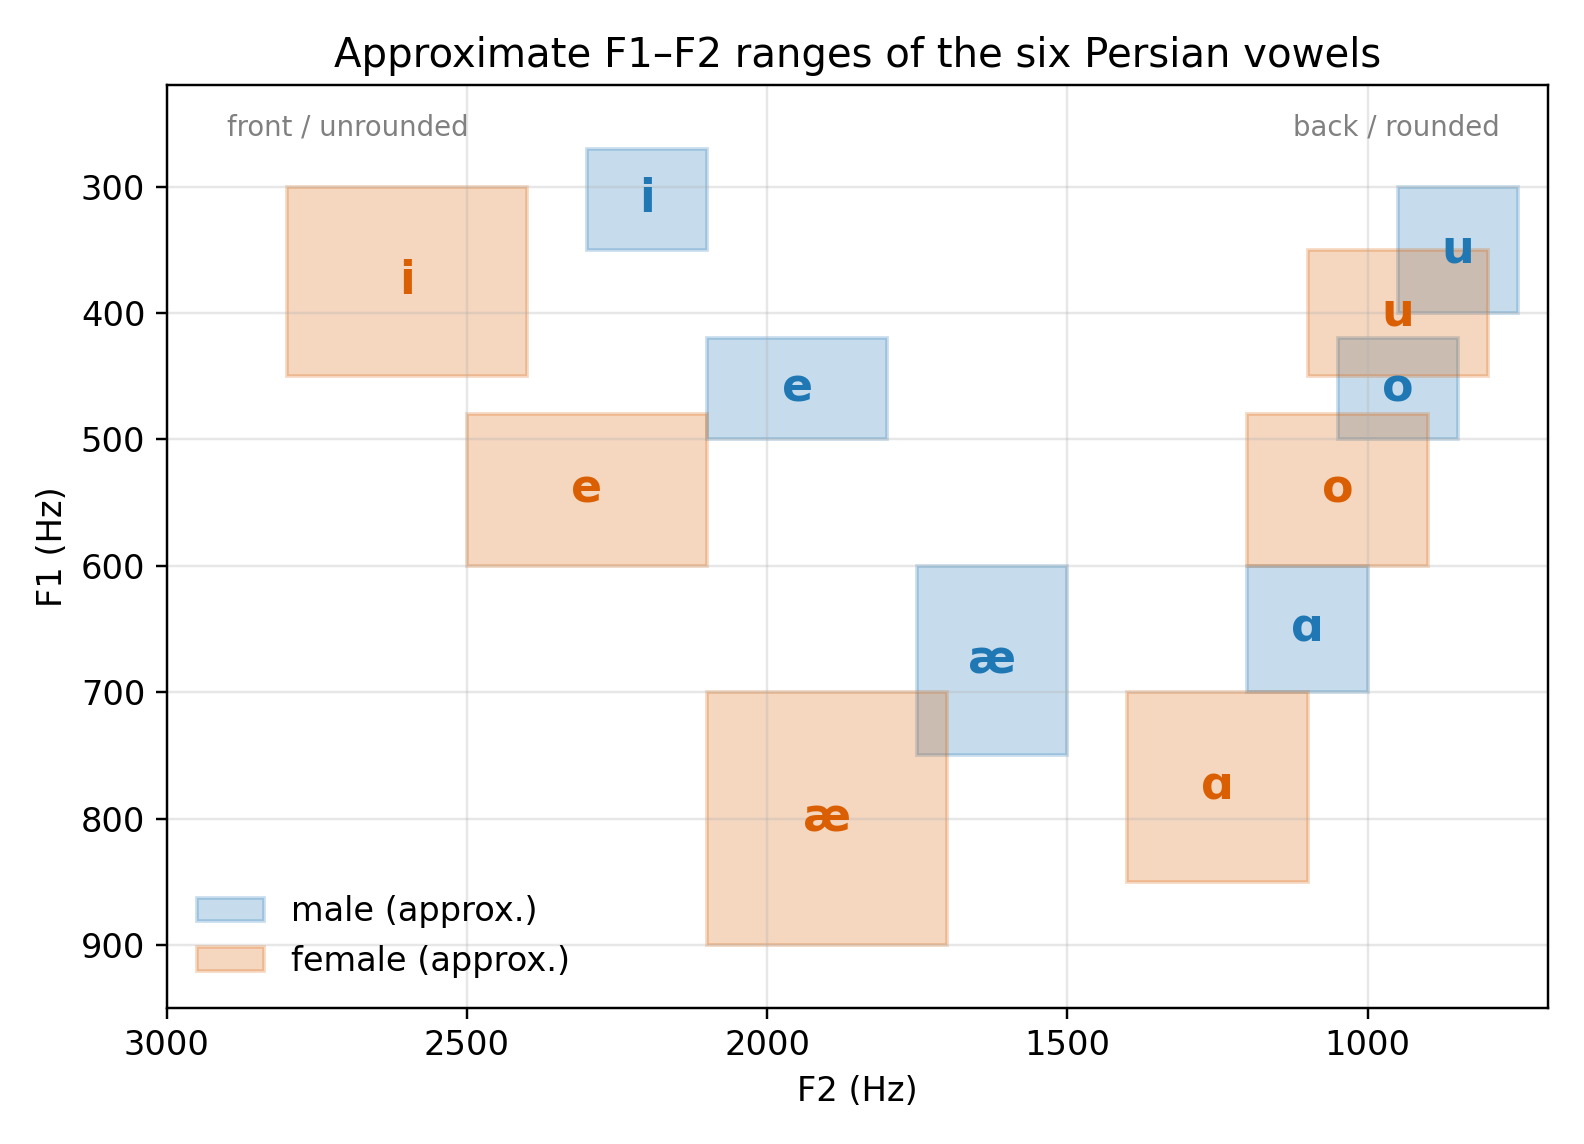
\includegraphics[width=0.75\textwidth]{../assets/figures/ch04-persian-vowel-chart.png}
  \caption{نمودار \eng{F1–F2} شش واکهٔ فارسی بر پایهٔ جدول بالا؛ مستطیل‌ها دامنهٔ مردان (آبی) و زنان (نارنجی) را نشان می‌دهند. محورها معکوس و مقادیر تقریبی‌اند (شکل افزوده).}
\end{figure}

\subsection{تفاوت فضای واکه‌ای در گروه‌های مختلف}
فضای واکه‌ای برای همه یکسان نیست و می‌توان آن را جداگانه برای کودکان و بزرگسالان، زنان و مردان، زبان‌های مختلف و افراد دارای اختلال گفتار استخراج کرد. انتظار داریم رابطهٔ کلی «\eng{F1} با ارتفاع و \eng{F2} با جلوآمدگی» حفظ شود، اما دامنهٔ عددی و پراکندگی تغییر کند. برای مقایسهٔ بین گویندگان معمولاً فرمنت‌ها نرمال می‌شوند، مثلاً با روش \eng{Lobanov}: $z=(F-\mu)/\sigma$ برای هر گوینده و هر فرمنت.

\subsection{مساحت فضای واکه‌ای (\eng{VSA})}
برای تبدیل «گستردگی فضای واکه‌ای» به یک عدد، مساحت چندضلعی واکه‌های گوشه در نمودار \eng{F1–F2} را حساب می‌کنیم (مقالهٔ \eng{Sandoval} و همکاران، ۲۰۱۳: چهار واکهٔ گوشه یا سه واکهٔ \eng{/a, i, u/} برای مثلث، با اندازه‌گیری در ۵۰ درصد مدت واکه و میانگین‌گیری). \eng{VSA} نمایندهٔ آکوستیکی جابه‌جایی اندام‌های گفتار است و در گفتار واضح‌تر بزرگ‌تر است.

\begin{definitionbox}{محاسبهٔ \eng{VSA} با فرمول شوله‌یس (\eng{Shoelace})}
اگر رأس‌های چندضلعی با ترتیب پیرامونی $(F_{2,k},F_{1,k})$ باشند:
\[
\text{\lr{VSA}}=\frac12\left|\sum_{k=1}^{n}\bigl(F_{2,k}\,F_{1,k+1}-F_{2,k+1}\,F_{1,k}\bigr)\right|\quad(\text{Hz}^2),\qquad k=n+1\equiv 1.
\]
برای مثلث \eng{(i, a, u)}:
\[
\text{\lr{VSA}}_{\triangle}=\frac12\left|F_{1,i}(F_{2,a}-F_{2,u})+F_{1,a}(F_{2,u}-F_{2,i})+F_{1,u}(F_{2,i}-F_{2,a})\right|.
\]
\end{definitionbox}

\begin{addedbox}{مثال عددی: \eng{VSA} مثلثی مردان فارسی‌زبان}
مرکز دامنه‌های جدول مردان: \eng{/i/} با $(F_1,F_2)=(310,\,2200)$، \eng{/ɑ/} با $(650,\,1100)$ و \eng{/u/} با $(350,\,850)$ هرتز.
\begin{align*}
\text{\lr{VSA}}_{\triangle}&=\tfrac12\bigl|310(1100-850)+650(850-2200)+350(2200-1100)\bigr|\\
&=\tfrac12\bigl|77\,500-877\,500+385\,000\bigr|=207\,500\ \text{Hz}^2.
\end{align*}
\textbf{اثر متمرکزشدن:} اگر هر فاصله از مرکز ثقل ۲۰ درصد کم شود (ضریب $0.8$)، چون مساحت با مربع ضریب مقیاس عوض می‌شود، مساحت جدید $0.8^2\times207\,500=132\,800\ \text{Hz}^2$ است، یعنی حدود ۳۶ درصد کاهش. پس \eng{VSA} به متمرکز شدن واکه‌ها حساس است. (شاخص نسبتی \eng{VAI} از \eng{Sapir} و همکاران ۲۰۱۰ برای کاهش وابستگی به اندازهٔ مجرا پیشنهاد شده و با متمرکزشدن کاهش می‌یابد.)
\end{addedbox}

\section{همخوان‌ها در اسپکتروگرام}
یکی از دانشجویان پرسید آیا این تحلیل فقط برای واکه‌هاست. پاسخ استاد: همخوان‌ها هم ویژگی‌های آکوستیکی خاص خود را دارند و در اسپکتروگرام قابل بررسی‌اند، اما تمرکز فعلی روی واکه‌هاست.

\begin{assignmentbox}{تمرین پیشنهادی استاد}
بررسی کنید همخوان‌ها چگونه در اسپکتروگرام دیده می‌شوند و آیا با آواشناسی تولیدی هماهنگ‌اند. روی تخته: اسپکتروگرام با \textbf{سکوت} (شیوهٔ تولید) و نحوهٔ \textbf{خم‌شدن و جهش فرمنت‌ها} و \textbf{مرکز فرکانسی نویز} (جایگاه تولید)، حرکات فیزیکی اندام‌های گفتاری را کدگذاری می‌کند. به‌خصوص این موارد را ببینید:
\begin{itemize}
  \item سکوت یا انسداد پیش از برخی همخوان‌ها؛
  \item انفجار (\eng{Burst}) در انسدادی‌هایی مانند \eng{/b/} و \eng{/p/};
  \item تغییر شکل فرمنت‌ها هنگام گذار از همخوان به واکه (\eng{Formant Transitions}).
\end{itemize}
\end{assignmentbox}

\section{کاربردهای فضای واکه‌ای}
استاد از دانشجویان پرسید فضای واکه‌ای چه کاربردی دارد. پاسخ‌های اولیه (تشخیص واکه، پیش‌پردازش) کافی نبود: فضای واکه‌ای قبل از هر چیز ابزار \emph{تحلیل ساختار تولید گفتار}، مقایسهٔ گروه‌ها و شناسایی الگوهای متفاوت است. سه کاربرد اصلی روی تخته بود.

\subsection{گفتاردرمانی و بازخورد زیستی تصویری}
در \term{بیوفیدبک تصویری}{Visual Biofeedback} برای کودکان دارای اختلال گفتار، ناشنوایان یا افراد مبتلا به سندرم داون، نمایشگری زنده نقطهٔ \eng{F1–F2} گفتار فرد را نشان می‌دهد و او می‌کوشد آن را با حرکت زبان به ناحیهٔ هدف برساند. مزیت: بازخورد از حالت صرفاً شنیداری به دیداری درمی‌آید. در گفتار کودکان و زنان ($f_0$ بالا) تخمین فرمنت ناپایدار است، پس بهتر است هدف را یک \emph{ناحیه} (بیضی دامنهٔ واکه) بگیریم، نه نقطه.

\subsection{تشخیص صدای جعلی (\eng{Deepfake})}
صدای سنتزشده می‌تواند برای گوش طبیعی باشد، اما این به معنای یکسان‌بودن همهٔ ویژگی‌های آکوستیکی و تولیدی با گفتار واقعی نیست. ایده: فرمنت‌های واکه‌ها را برای نمونهٔ واقعی و سنتزشده استخراج و فضای واکه‌ای (و هم‌بستگی الگوی تغییر \eng{F1} و \eng{F2}) را مقایسه کنیم. روی تخته: «تفاوت‌های بیومکانیکی در تلفظ مصوت‌ها بهترین ردپای مصنوعی‌بودن صدا هستند».

\begin{figure}[htbp]
  \centering
  \fbox{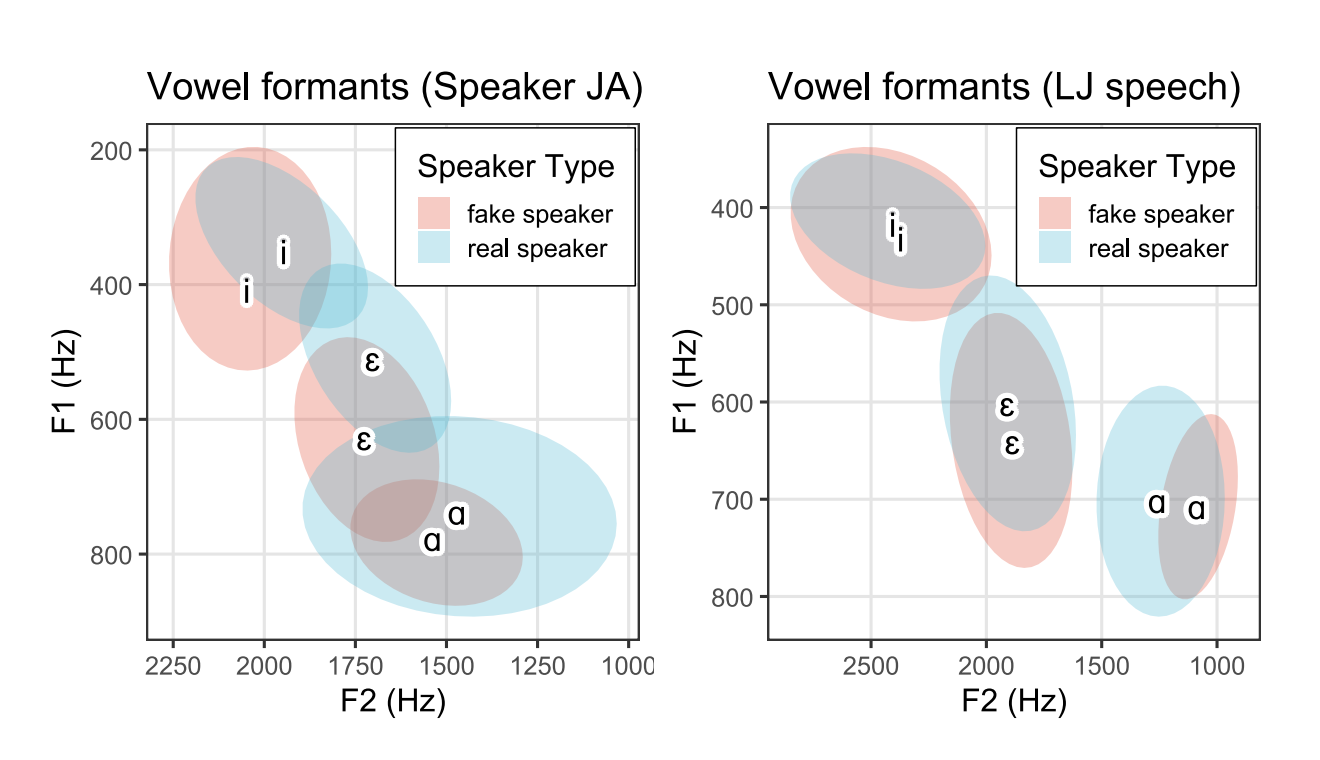
\includegraphics[width=0.55\textwidth]{../assets/figures/ch04-fake-real-vowels.png}}
  \caption{بیضی‌های \eng{F1–F2} چند واکه در صدای واقعی (آبی) و جعلی (قرمز) برای دو گوینده/پیکره، از مقالهٔ \eng{Conditional Speaker Normalization of Vocal Tract Shape Features for Robust Synthetic Speech Detection} (\eng{IEEE Access}، ۲۰۲۶) \textit{(برگرفته از تختهٔ کلاس)}}
\end{figure}

\begin{correctionbox}{«اثبات» جعل؟}
این روش‌ها شواهد آماری تولید می‌کنند، نه اثبات قطعی؛ در نمودار هم بسیاری از بیضی‌های واقعی و جعلی هم‌پوشانی زیادی دارند. استاد تأکید کرد گزارهٔ کلی «فرمنت‌ها فرق دارند» برای پژوهش کافی نیست؛ باید معلوم شود: (۱) دقیقاً کدام ویژگی تفاوت دارد، (۲) چگونه اندازه‌گیری می‌شود، (۳) آیا تکرارپذیر است، (۴) آیا تفکیک قابل‌اعتماد می‌دهد.
\end{correctionbox}

\textbf{مقاوم‌سازی مدل (\eng{Robustness}):} اگر نقاط ضعف مدل را بشناسیم (مثلاً ضعف در برخی واکه‌ها)، از همان داده‌ها بیشتر جمع می‌کنیم؛ روش‌های مرتبط: \eng{Data Augmentation}، \eng{Hard Example Mining} و \eng{Adversarial Training}. تحلیل فضای واکه‌ای می‌تواند یکی از راه‌های شناسایی این نقاط باشد.

\subsection{نشانگر زیستی دیجیتال (\eng{Digital Biomarker})}
\begin{definitionbox}{نشانگر زیستی دیجیتال}
ویژگی قابل‌اندازه‌گیری‌ای که با ابزارهای دیجیتال به دست می‌آید و دربارهٔ وضعیت یا تغییرات یک فرایند زیستی یا بالینی اطلاعات می‌دهد؛ مثلاً ویژگی‌های آکوستیکی گفتار برای دنبال‌کردن بیماری‌های عصبی مانند پارکینسون و دمانس.
\end{definitionbox}

در این بیماری‌ها \eng{F1} و \eng{F2} واکه‌ها به سمت مرکز فضای صوتی جمع می‌شوند (\term{متمرکزشدن}{Centralization}) و مساحت فضای واکه‌ای کوچک می‌شود. اندازه‌گیری مکرر در طول زمان می‌تواند تغییراتی را نشان دهد که شنوندهٔ عادی هنوز نمی‌شنود. روند پایش: ضبط دوره‌ای واکه‌ها یا جمله‌های ثابت $\leftarrow$ استخراج فرمنت $\leftarrow$ ساخت فضای واکه‌ای و اندازه‌گیری گستردگی $\leftarrow$ مقایسه با نمونه‌های قبلی همان فرد $\leftarrow$ در صورت تغییر قابل‌توجه، ارجاع به متخصص. استاد ایدهٔ سامانه‌ای مبتنی بر \textbf{تلفن همراه} برای این پایش را مطرح کرد. (مقالهٔ \eng{Sandoval} الگوریتمی برای تخمین خودکار \eng{VSA} از گفتار پیوسته ارائه می‌کند.)

\begin{figure}[htbp]
\centering
\begin{tikzpicture}[rtl, scale=1.0]
  \begin{scope}[xshift=6cm]
    \draw[fill=blue!15, draw=blue!60!black, thick] (0,0) -- (3,0.2) -- (2.3,2.5) -- cycle;
    \node[font=\small] at (1.8,-0.55) {فضای گسترده};
    \node[font=\small] at (1.8,-1.05) {تمایز بیشتر واکه‌ها};
    \node[font=\scriptsize] at (-0.2,-0.2) {\lr{/i/}};
    \node[font=\scriptsize] at (3.3,0.2) {\lr{/u/}};
    \node[font=\scriptsize] at (2.3,2.8) {\lr{/a/}};
  \end{scope}
  \begin{scope}
    \draw[fill=orange!20, draw=orange!70!black, thick] (0.8,0.65) -- (2.2,0.75) -- (1.9,1.7) -- cycle;
    \node[font=\small] at (1.5,-0.55) {فضای متمرکز};
    \node[font=\small] at (1.5,-1.05) {کاهش فاصلهٔ واکه‌ها};
    \node[font=\scriptsize] at (0.5,0.55) {\lr{/i/}};
    \node[font=\scriptsize] at (2.5,0.75) {\lr{/u/}};
    \node[font=\scriptsize] at (1.9,2.0) {\lr{/a/}};
  \end{scope}
  \draw[-{Stealth}, thick] (5.2,1.0) -- (3.9,1.0);
\end{tikzpicture}
\caption{نمایش شماتیک متمرکزشدن فضای واکه‌ای: مثلث واکه‌ها کوچک می‌شود و به مرکز نزدیک می‌شود (شکل افزوده).}
\end{figure}

\begin{correctionbox}{نشانگر زیستی دیجیتال ابزار تشخیص قطعی نیست}
شواهد پژوهشی کاهش \eng{VSA} یا \eng{VAI} را در برخی افراد مبتلا به پارکینسون و سایر دیزآرتری‌های حرکتی نشان می‌دهند، ولی اثر آن در همهٔ بیماران و مراحل یکسان نیست و برای دمانس شواهد ضعیف‌تر است. این شاخص‌ها به‌تنهایی تشخیص قطعی نیستند و به اعتبارسنجی بالینی و تفسیر متخصص نیاز دارند؛ سن، جنس، خستگی، کیفیت میکروفون و نویز نیز \eng{VSA} را تغییر می‌دهند.
\end{correctionbox}

\section{جمع‌بندی}
با اندازه‌گیری \eng{F1} و \eng{F2} در \eng{Praat} می‌توان بازنمایی‌ای از الگوی تولید واکه‌ها ساخت. با برچسب‌گذاری \eng{TextGrid} و بازهٔ هر واکه، جدول فرمنت‌ها برای هر گروه تهیه و در نمودار \eng{F1–F2} با محورهای معکوس فضای واکه‌ای شکل می‌گیرد. این بازنمایی امکان مقایسهٔ گروه‌ها، گفتاردرمانی تصویری، تشخیص صدای مصنوعی و پایش تغییرات گفتار را می‌دهد، اما همهٔ این کاربردها اعتبارسنجی دقیق و تفسیر محتاطانه می‌خواهند.

\begin{exambox}{نکات مهم برای مرور و امتحان}
\begin{center}
\small
\begin{tabular}{p{3.6cm}p{10cm}}
\toprule
مفهوم & نکتهٔ اصلی \\
\midrule
فرکانس پایه و \eng{Magnitude} & $f_0=1/T$، مربوط به منبع؛ \eng{Magnitude} اندازهٔ ضریب فوریه است، نه دامنهٔ زمانی \\
تعامد و هارمونیک‌ها & ضرب داخلی صفر؛ هارمونیک‌ها مضرب‌های صحیح $f_0$ (موج مربعی: فقط فرد) \\
فرمنت‌ها & نواحی تشدید مجرا (فیلتر)؛ تخمین با \eng{LPC} \\
\eng{Wideband} / \eng{Narrowband} & تفکیک زمانی (فرمنت) در برابر تفکیک فرکانسی (هارمونیک) \\
\eng{F1} و \eng{F2} & \eng{F1} معکوس با ارتفاع زبان؛ \eng{F2} مستقیم با جلو آمدن زبان و کاهش‌یافته با گردی لب \\
\eng{Praat} و \eng{TextGrid} & ضبط، تحلیل و استخراج فرمنت؛ لایه‌های \eng{Word}، \eng{Syllable}، \eng{Phoneme} \\
فضای واکه‌ای & نمودار \eng{F1–F2} با هر دو محور معکوس؛ برای هر گروه جداگانه \\
\eng{ASR} + بازبینی انسانی & ساخت سریع‌تر پیکره؛ مستندسازی برچسب‌گذاری ضروری \\
\eng{VSA} & مساحت چندضلعی واکه‌های گوشه؛ کوچک‌شدن = متمرکزشدن \\
کاربردها & گفتاردرمانی (بیوفیدبک تصویری)، تشخیص جعل، نشانگر زیستی دیجیتال \\
\bottomrule
\end{tabular}
\end{center}
\textbf{زنجیرهٔ جلسه:} سیگنال صوتی $\leftarrow$ ویژگی‌های آکوستیکی (\eng{Pitch}، طیف، فرمنت) $\leftarrow$ اندازه‌گیری \eng{F1}/\eng{F2} در \eng{Praat} $\leftarrow$ ساخت فضای واکه‌ای $\leftarrow$ مقایسه با مرجع یا گروه‌های دیگر $\leftarrow$ کاربردهای پژوهشی و عملی.
\end{exambox}

\chapter{ادراک شنیداری، مقیاس مل و ضرایب \eng{MFCC}}

تا اینجا سیگنال گفتار را از دید فیزیکی بررسی کردیم (شکل موج، فوریه، هارمونیک، فرمنت، فضای واکه‌ای) و طیفی دیدیم که همهٔ فرکانس‌ها را یکسان می‌دید. در این جلسه ویژگی‌های \term{سیستم شنوایی انسان}{Human Auditory System} را وارد استخراج ویژگی می‌کنیم. حاصل کار مقیاس مل، بانک فیلتر مل، لگاریتم و در نهایت \term{ضرایب کپسترال فرکانس مل}{Mel-Frequency Cepstral Coefficients} یا \eng{MFCC} است که در جلسات بعد هم بارها به آن برمی‌گردیم.

\begin{exambox}{نقشهٔ راه جلسه}
(۱) چرا شنوایی را مدل کنیم؟ (۲) نقشهٔ تونوتوپیک حلزون؛ (۳) مقیاس مل و بانک فیلتر مثلثی؛ (۴) لگاریتم برای ادراک غیرخطی بلندی؛ (۵) افزونگی ویژگی‌ها، \eng{DCT} و پیدایش \eng{MFCC}؛ (۶) کپستروم؛ (۷) کاربردها و رابطهٔ \eng{MFCC} با یادگیری ماشین.
\end{exambox}

%====================================================================
\section{چرا باید ادراک شنیداری انسان را در نظر بگیریم؟}
%====================================================================

تبدیل فوریه می‌گوید هر مؤلفهٔ فرکانسی چه سهمی دارد، بی‌آنکه بپرسد انسان کدام فرکانس‌ها را بهتر تشخیص می‌دهد. انسان جوان و سالم صداهایی را در حدود \textbf{۲۰ هرتز تا ۲۰ کیلوهرتز} می‌شنود، و باید دو چیز را از هم جدا کرد:
\begin{itemize}
  \item \textbf{وجود فیزیکی ارتعاش}: پدیده‌ای که طبق قوانین فیزیک رخ می‌دهد؛
  \item \textbf{ادراک شنیداری ارتعاش}: فرایندی که ارتعاش را از دستگاه شنوایی عبور می‌دهد و در مغز به تجربهٔ شنیدن تبدیل می‌کند.
\end{itemize}
مثال کلاس از بینایی: چراغی که با فرکانس بسیار زیاد چشمک می‌زند را پیوسته روشن می‌بینیم، هرچند از نظر فیزیکی همچنان خاموش و روشن می‌شود.

%====================================================================
\section{نقشهٔ تونوتوپیک حلزون گوش}
%====================================================================

صدا از گوش خارجی و میانی می‌گذرد و در \term{حلزون گوش}{Cochlea} موجی روی \term{غشای پایه}{Basilar Membrane} پدید می‌آورد. نقاط مختلف این غشا به فرکانس‌های مختلف حساس‌اند؛ به این سازمان‌دهی \term{نقشهٔ تونوتوپیک}{Tonotopic Map} می‌گویند.

\begin{figure}[htbp]
  \centering
  \fbox{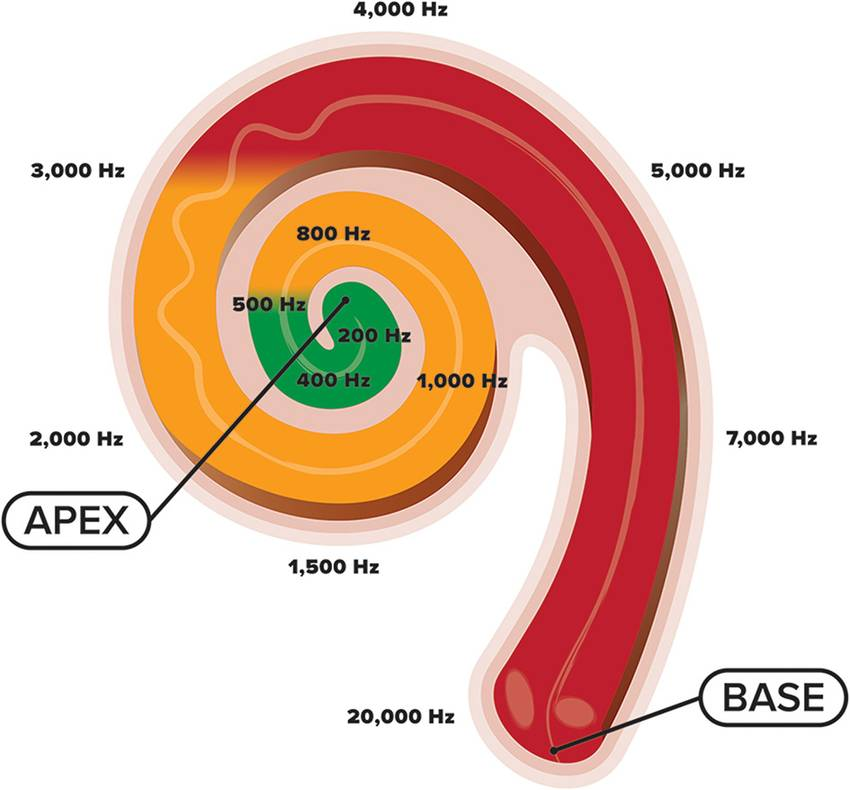
\includegraphics[width=0.46\textwidth]{../assets/figures/ch05-cochlea-tonotopic.png}}\hspace{0.03\textwidth}
  \fbox{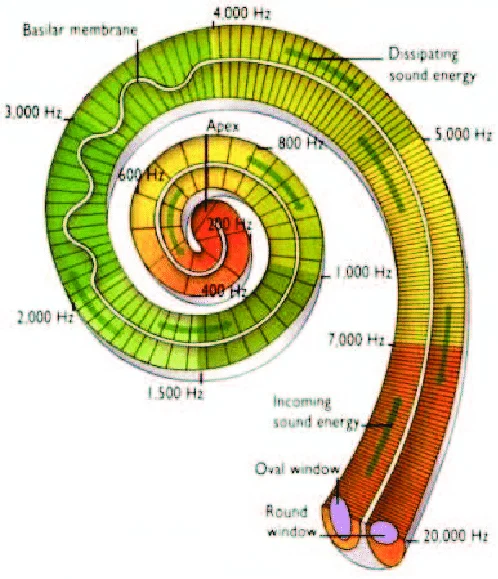
\includegraphics[width=0.38\textwidth]{../assets/figures/ch05-basilar-membrane.png}}
  \caption{نقشهٔ تونوتوپیک حلزون گوش. رأس (\eng{Apex}) مربوط به فرکانس‌های بم و قاعده (\eng{Base}) نزدیک دریچه‌های بیضی و گرد مربوط به فرکانس‌های زیر است. \textit{(برگرفته از تختهٔ کلاس)}}
  \label{fig:cochlea}
\end{figure}

\begin{correctionbox}{دقت در خواندن شکل}
عدد نزدیک رأس (حدود ۲۰۰ هرتز) حد پایین واقعی شنوایی نیست؛ شنوایی تا حدود ۲۰ هرتز ادامه دارد. همچنین فاصلهٔ مکانی روی غشای پایه تقریباً با \emph{لگاریتم فرکانس} متناسب است (نه خطی)؛ همین ریشهٔ فیزیولوژیک مقیاس مل است.
\end{correctionbox}

\subsection{تفکیک نابرابر فرکانس‌های بم و زیر}
ادراک تغییرات فرکانسی خطی نیست. دو تغییر $100\to200$ هرتز و $5100\to5200$ هرتز هر دو ۱۰۰ هرتز اختلاف دارند، اما اولی برای گوش چشمگیر و دومی تقریباً نامحسوس است؛ یعنی تفاوت ادراکی به \emph{محدودهٔ فرکانسی} هم بستگی دارد، نه فقط به اختلاف عددی. مثال‌های کلاس: تغییر کوچک در صدای موتور (فرکانس پایین) به‌سادگی شنیده می‌شود، ولی تغییر کوچک فرکانس یک سوت (فرکانس بالا) دشوارتر. گوش در فرکانس‌های پایین (زیر حدود ۱۰۰۰ هرتز) بسیار دقیق است و در فرکانس‌های بالا (بالای حدود ۴۰۰۰ هرتز) کمتر.

\begin{correctionbox}{دقت علمی}
در فرکانس‌های بالا تفکیک گوش تقریباً نسبت‌محور است. تغییر ۱۰۰ هرتز در ۵ کیلوهرتز برای شنوندهٔ آموزش‌دیده هنوز قابل‌تشخیص است؛ درست‌تر این است که از نظر ادراکی \emph{بسیار کوچک‌تر} از تغییر ۱۰۰ به ۲۰۰ هرتز به‌نظر می‌رسد. مقیاس مل همین را مدل می‌کند.
\end{correctionbox}

\textbf{پیامد:} در فرکانس‌های پایین بازه‌های باریک و در بالا بازه‌های پهن‌تر می‌خواهیم؛ این مبنای مقیاس مل است.

%====================================================================
\section{مرور سه ویژگی \eng{Pitch}، \eng{Formant} و \eng{Intensity} در \eng{Praat}}
%====================================================================

استاد روی یک سیگنال در \eng{Praat} (فرمنت‌ها: نقطه‌های قرمز؛ \eng{pitch}: خط آبی؛ شدت: خط زرد) سه ویژگی را مرور کرد:
\begin{itemize}
  \item \term{فرمنت}{Formant}: نواحی تشدید طیفی ($F_1$، $F_2$، $F_3$) که برای ساخت فضای واکه‌ای به کار رفتند.
  \item \term{پیچ}{Pitch}: ادراک زیر و بمی؛ با فرکانس پایه $F_0$ (کمیت فیزیکی، تناوب سیگنال) مرتبط است ولی با آن یکی نیست.
  \item \term{شدت}{Intensity}: معیار قدرت کلی صوت در هر لحظه (فریاد: شدت زیاد، صحبت آرام: شدت کم).
\end{itemize}

\begin{table}[htbp]
\centering
\caption{کمیت‌های فیزیکی و ادراکی که باید از هم جدا نگه داشته شوند.}
\begin{tabular}{p{4cm}p{4.5cm}p{4cm}}
\toprule
\textbf{کمیت فیزیکی} & \textbf{کمیت ادراکی} & \textbf{توضیح} \\
\midrule
فرکانس پایه \eng{($F_0$)} & زیر و بمی (\eng{Pitch}) & تناوب موج در برابر احساس زیر/بم \\
شدت (\eng{Intensity}) & بلندی (\eng{Loudness}) & توان فیزیکی در برابر بلندی احساس‌شده \\
فرمنت‌ها / شکل طیف & رنگ صدا (\eng{Timbre}) & تشدیدهای مجرای صوتی \\
\bottomrule
\end{tabular}
\end{table}

زیر و بمی با بلندی یکی نیست: می‌توان با صدای زیر ولی آرام، یا بم و پرشدت صحبت کرد.

\begin{exambox}{پرسش و پاسخ: چرا خط \eng{pitch} گاهی بالاتر از نقطه‌های فرمنت است؟}
چون این نمودارها با \emph{محورهای مختلف} (یک مقیاس برای \eng{pitch}، یکی برای فرمنت) روی یک تصویر رسم می‌شوند؛ بالاتر بودن خط روی صفحه دلیل بزرگ‌تر بودن مقدار فرکانسی نیست. نحوهٔ محاسبهٔ کانتور این ویژگی‌ها جلسهٔ بعد بررسی می‌شود.
\end{exambox}

%====================================================================
\section{کم‌شنوایی فرکانس‌های بالا با افزایش سن}
%====================================================================

چون قاعدهٔ حلزون به فرکانس‌های بالا مربوط است، آسیب به آن شنیدن صداهای زیر را کم می‌کند؛ کم‌شنوایی فرکانس‌های بالا در سنین بالا رایج است و \term{پیرگوشی}{Presbycusis} نام دارد. توضیح کلاس: سلول‌های ناحیهٔ قاعده در «خط مقدم» ضربه‌های مکانیکی‌اند و زودتر تحلیل می‌روند.

\begin{correctionbox}{دقت علمی}
الگوی کلی درست است، اما علت آن چندعاملی است (از دست رفتن سلول‌های مویی، تحلیل رگ‌ها، نورون‌های عصب شنوایی، نویز، ژنتیک و غیره)؛ توضیح کلاس را «سازوکارهای محتمل» بدانید نه علت قطعی. نمونهٔ عملی: همخوان‌های بی‌واک مانند \eng{/s/} و \eng{/f/} انرژی‌شان در فرکانس‌های بالاست و برای افراد دچار پیرگوشی سخت‌تر تفکیک می‌شوند.
\end{correctionbox}

%====================================================================
\section{مقیاس مل}
%====================================================================

\begin{definitionbox}{مقیاس مل}
\term{مقیاس مل}{Mel Scale} یک \textbf{نگاشت غیرخطی} از فرکانس فیزیکی (هرتز) به مقیاس ادراکی (مل) است که فرکانس‌های بالا را «فشرده» می‌کند تا فاصله‌های برابر روی محور مل تقریباً با تفاوت‌های ادراکی برابر در زیر و بمی متناظر باشند. نام آن از \eng{melody} گرفته شده است.
\end{definitionbox}

\begin{correctionbox}{فرمول مقیاس مل}
مقیاس مل را استیونز، فولکمن و نیومن (۱۹۳۷) از آزمایش‌های قضاوت زیر و بمی معرفی کردند. رایج‌ترین تقریب تحلیلی (که در کلاس به‌صورت عددی بیان نشد):
\[
m = 2595\,\log_{10}\!\Big(1+\frac{f}{700}\Big)
\qquad\Longleftrightarrow\qquad
f = 700\big(10^{\,m/2595}-1\big).
\]
۱۰۰۰ هرتز به ۱۰۰۰ مل نگاشت می‌شود. قراردادهای دیگری هم وجود دارد (مثلاً نسخهٔ اسلینی)، پس خروجی کتابخانه‌ها ممکن است اندکی فرق کند.
\end{correctionbox}

تابع در فرکانس‌های پایین (زیر حدود ۱ کیلوهرتز) تقریباً خطی و در فرکانس‌های بالاتر لگاریتمی است.

\begin{figure}[htbp]
  \centering
  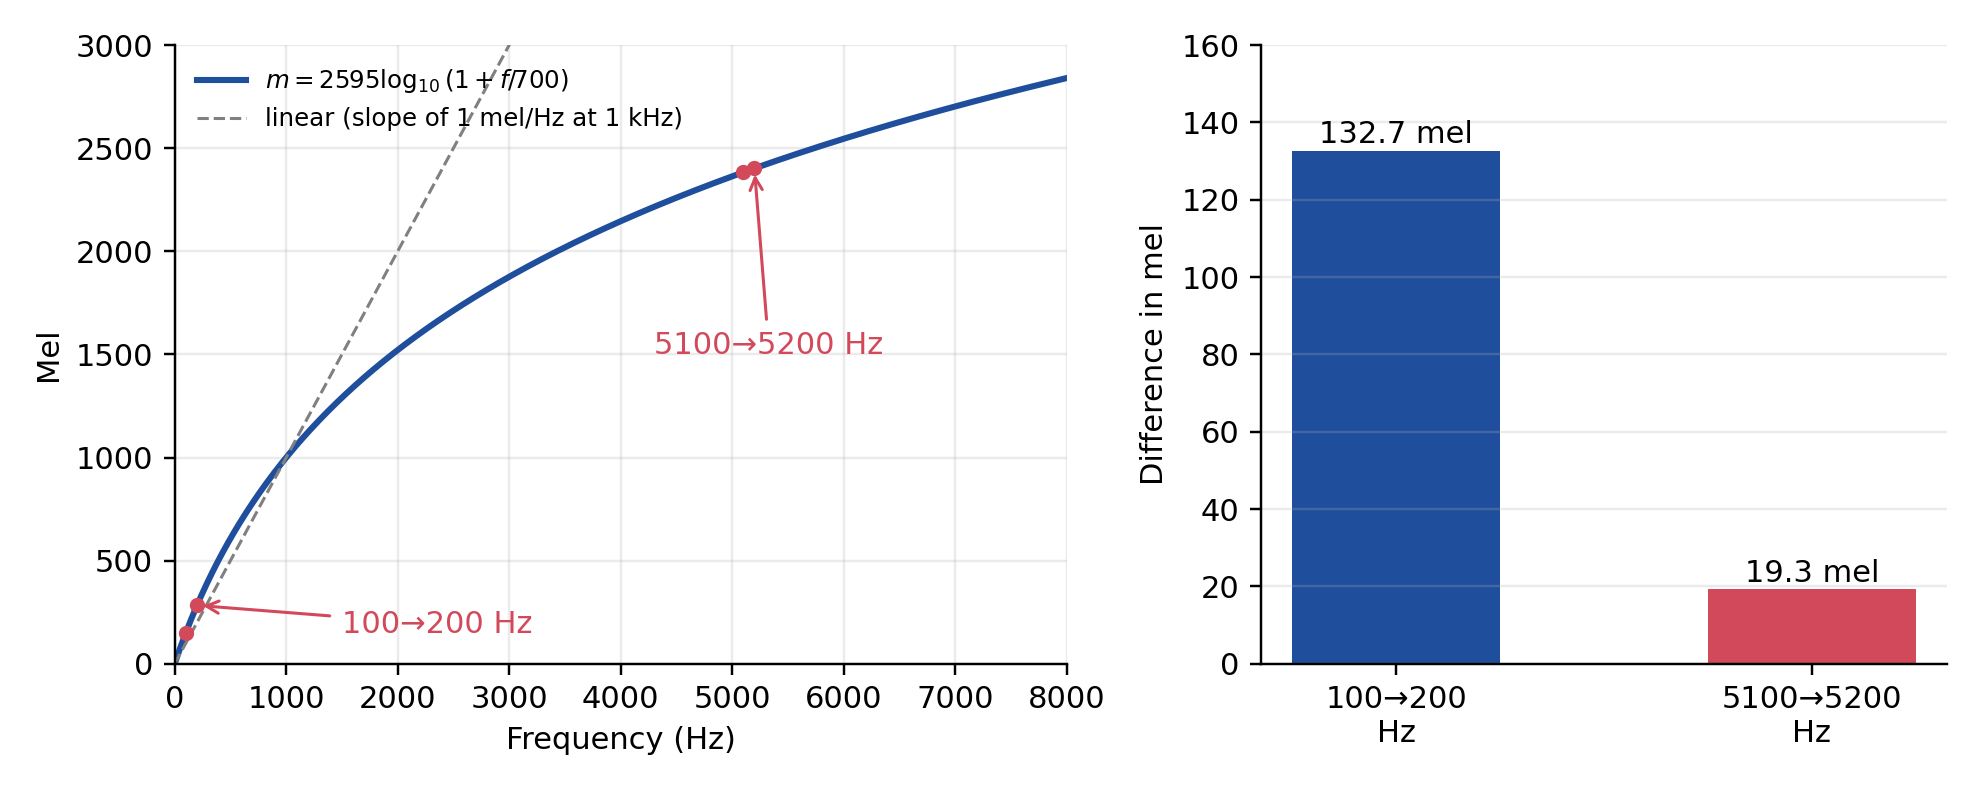
\includegraphics[width=0.95\textwidth]{../assets/figures/ch05-mel-vs-hz.png}
  \caption{چپ: منحنی تبدیل هرتز به مل. راست: همان دو تغییر ۱۰۰ هرتزی در مقیاس مل ($132.7$ مل در برابر $19.3$ مل). (شکل افزوده)}
  \label{fig:melcurve}
\end{figure}

\begin{addedbox}{مثال عددی: تبدیل هرتز به مل}
\begin{center}
\begin{tabular}{rrrrrrr}
\toprule
$f$ (هرتز) & 100 & 200 & 1000 & 2000 & 5100 & 8000 \\
\midrule
$m$ (مل) & $150.5$ & $283.2$ & $1000.0$ & $1521.4$ & $2383.1$ & $2840.0$ \\
\bottomrule
\end{tabular}
\end{center}
بازهٔ ۰ تا ۸ کیلوهرتز فقط به حدود ۲۸۴۰ مل نگاشت می‌شود و نیمی از آن (۰ تا ۱۴۲۰ مل) زیر حدود ۱۷۶۰ هرتز است؛ یعنی مل به فرکانس‌های پایین «فضای بیشتری» می‌دهد.
\end{addedbox}

%====================================================================
\section{بانک فیلتر مل}
%====================================================================

\term{بانک فیلتر مل}{Mel Filterbank} مجموعه‌ای از فیلترهای مثلثی هم‌پوشان روی محور فرکانس است. هر فیلتر یک بازهٔ فرکانسی را پوشش می‌دهد و از آن \emph{یک عدد} (انرژی آن باند) می‌سازد.

\subsection{وزن‌دهی مثلثی}
وزن هر فیلتر در ابتدای بازه نزدیک صفر، در مرکز بیشینه (معمولاً ۱) و در انتها دوباره صفر است؛ پس فرکانس‌های نزدیک مرکز سهم بیشتری دارند. مقدار طیفی هر فرکانس در وزن متناظر ضرب و حاصل‌ها جمع می‌شوند:
\[
S_m=\sum_{k} H_m[k]\,P[k],
\]
که $P[k]$ طیف توان و $H_m[k]$ وزن فیلتر $m$ام است.

\begin{exambox}{مثال عددی کلاس: خروجی یک فیلتر}
فیلتری سه مؤلفهٔ طیفی با مقدارهای ۴، ۸ و ۶ و وزن‌های $0.5$، ۱ و $0.5$ دریافت می‌کند (اعداد آموزشی‌اند):
\[
M_1=(4\times0.5)+(8\times1)+(6\times0.5)=2+8+3=13 .
\]
به‌جای سه مقدار، یک عدد داریم؛ این کار برای همهٔ فیلترهای بانک تکرار می‌شود.
\end{exambox}

\subsection{چرا فیلترها هم‌پوشان‌اند؟}
تا اطلاعات فرکانس‌های نزدیک مرز دو باند ناگهان حذف یا دچار پرش نشود. مثال تخته: اگر مرز دو باند ۳۰۰ هرتز و فیلترها مستطیلی بدون هم‌پوشانی باشند، تغییر ۱ هرتزی (۲۹۹ به ۳۰۱) مؤلفه را ناگهان از یک فیلتر به فیلتر دیگر می‌برد و خروجی‌ها می‌پرند؛ با مثلث‌های هم‌پوشان فقط تغییری هموار و کوچک رخ می‌دهد.

\subsection{چرا عرض فیلترها یکسان نیست؟}
مهم‌ترین نکتهٔ بانک فیلتر مل: روی محور \emph{خطی} فرکانس، فیلترها در فرکانس‌های پایین باریک و در فرکانس‌های بالا پهن‌اند (دقت در فرکانس‌های بالا کمتر است). دلیل: فیلترها روی \emph{محور مل} یکسان و هم‌فاصله‌اند و با بازگشت به هرتز در بالا پهن می‌شوند. این همان ایدهٔ نقشهٔ تونوتوپیک است.

\begin{figure}[htbp]
  \centering
  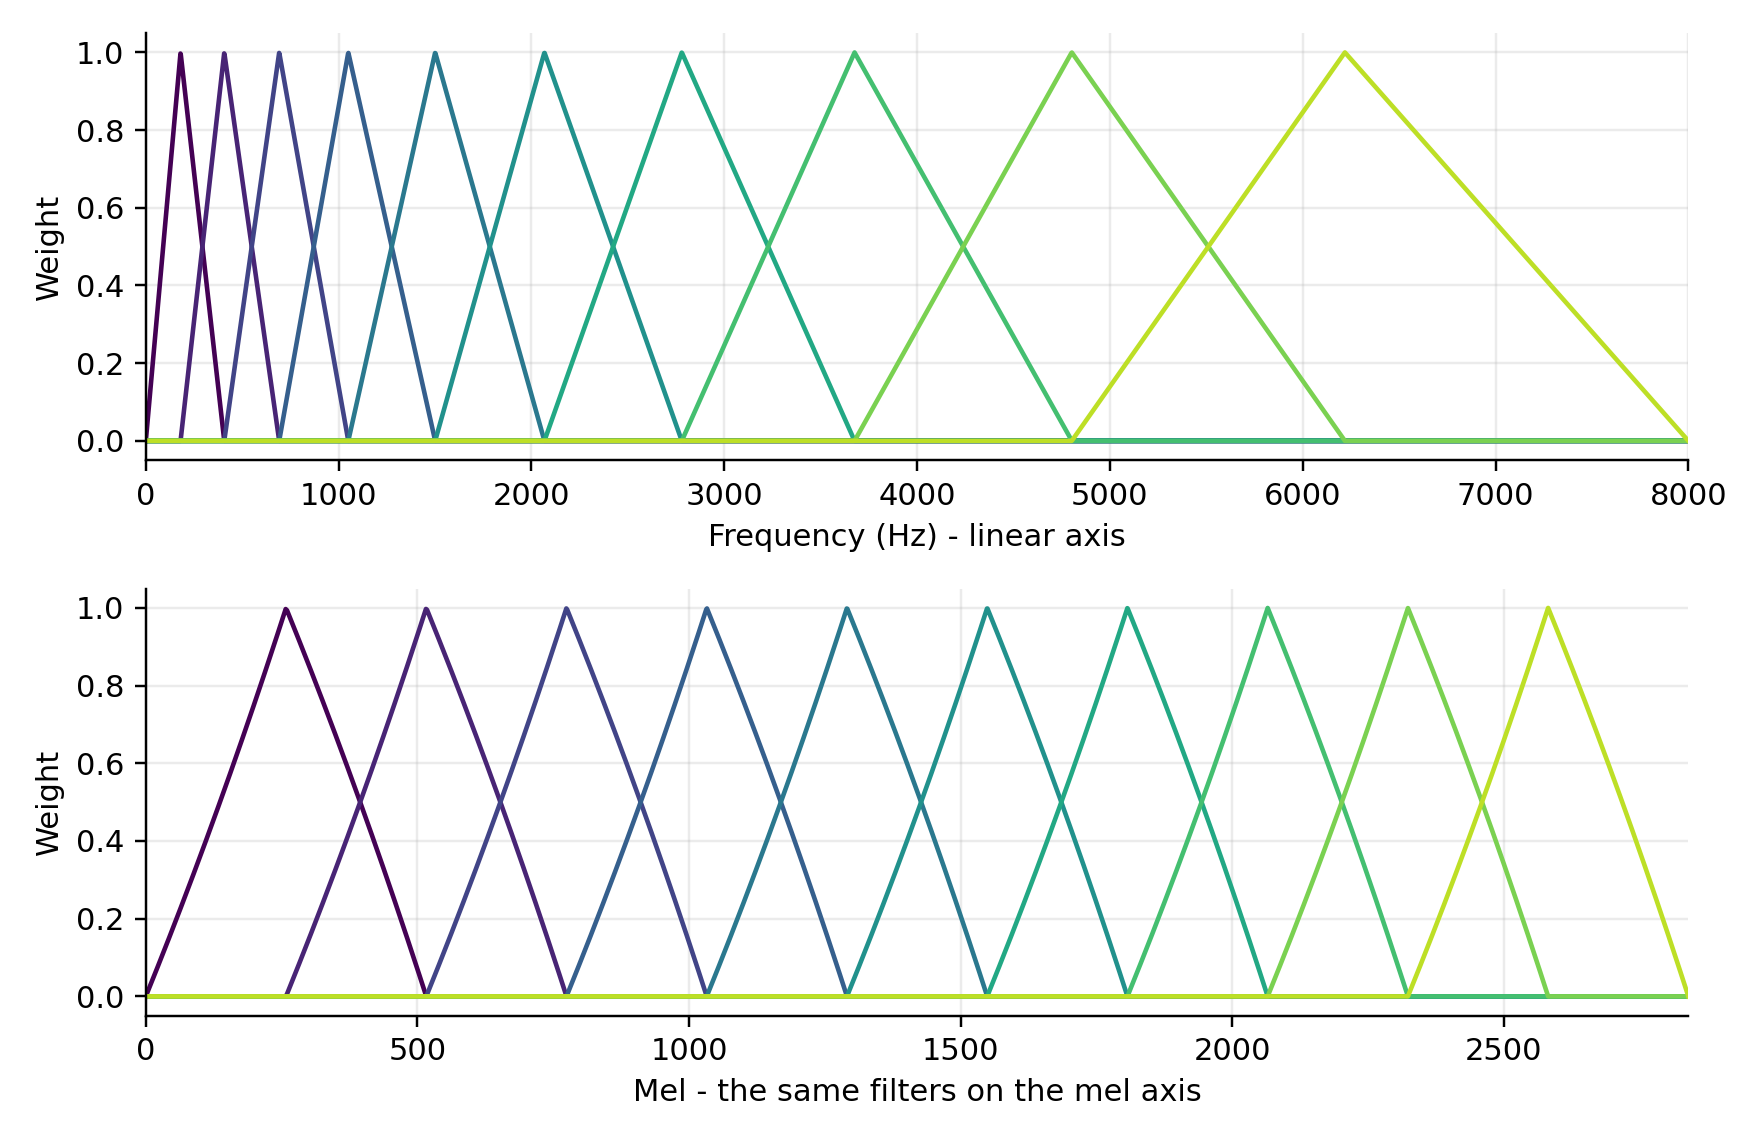
\includegraphics[width=0.9\textwidth]{../assets/figures/ch05-mel-filterbank.png}
  \caption{نمونهٔ یک بانک ده‌فیلتری برای بازهٔ ۰ تا ۸ کیلوهرتز. بالا: روی محور خطی هرتز فیلترها به‌تدریج پهن می‌شوند. پایین: همان فیلترها روی محور مل، مثلث‌هایی یکسان و هم‌فاصله‌اند. (شکل افزوده)}
  \label{fig:fbplot}
\end{figure}

\subsection{تعداد فیلترها}
در کلاس: حدود ۴۰ فیلتر مل رایج است و خروجی هر فریم یک بردار ۴۰‌تایی $\mathbf{M}=[M_1,\ldots,M_{40}]$ است. استاد تأکید کرد ۴۰ مقدار تجربی و متداول است، نه ثابت اجباری. 

\begin{correctionbox}{طیف توان یا اندازه؟}
در کلاس گفته شد اندازهٔ خروجی فوریه در مثلث‌ها ضرب می‌شود. هر دو دیده می‌شوند، اما در تعریف استاندارد \eng{MFCC} فیلترها روی \emph{طیف توان} (مربع اندازه، «انرژی هر باند») اعمال می‌شوند.
\end{correctionbox}

\begin{exambox}{پرسش و پاسخ: آیا با ادغام فرکانس‌ها اطلاعات از دست نمی‌رود؟}
چرا، عمداً اطلاعات را \emph{خلاصه} می‌کنیم. هدف نگه‌داشتن طیف اصلی نیست، ساختن نمایشی مناسب‌تر برای گفتار است: تفکیک ریز فرکانس‌های بالا از دید ادراک اهمیت کمتری دارد و هم‌پوشانی از حذف ناگهانی اطلاعات مرزی جلوگیری می‌کند.
\end{exambox}

%====================================================================
\section{ادراک غیرخطی بلندی صدا و لگاریتم}
%====================================================================

گوش در \emph{شدت} هم غیرخطی است: اگر شدت فیزیکی ۱۰۰ برابر شود، صدا را ۱۰۰ برابر بلندتر حس نمی‌کنیم، بلکه فقط چند برابر. این ویژگی به گوش اجازه می‌دهد با گسترهٔ بسیار وسیعی از شدت‌ها کار کند.

برای وارد کردن این ویژگی از خروجی هر فیلتر مل لگاریتم می‌گیریم:
\[
L_i=\log(M_i),\qquad \mathbf{L}=[\log M_1,\ldots,\log M_{40}].
\]
لگاریتم تغییرات بزرگ را فشرده می‌کند: $\log_{10}(10)=1$، $\log_{10}(100)=2$، $\log_{10}(1000)=3$؛ ورودی ۱۰۰ برابر شده ولی خروجی فقط از ۱ به ۳ رسیده است. در کلاس تأکید شد در این مرحله فقط روی \emph{شدت} لگاریتم می‌گیریم و به زیر و بمی کاری نداریم.

\begin{correctionbox}{لگاریتم، تقریبی از بلندی؛ نه خود بلندی}
لگاریتم مدلی ساده برای فشردگی بلندی است، نه رابطهٔ دقیق آن. قانون توانی استیونز می‌گوید بلندی تقریباً با $I^{0.3}$ متناسب است: ۱۰۰ برابر شدن شدت، بلندی را حدود $100^{0.3}\approx4$ برابر می‌کند.
\end{correctionbox}

\begin{warningbox}{لگاریتم صفر!}
اگر خروجی فیلتر صفر باشد (مثلاً سکوت دیجیتال)، $\log 0=-\infty$ می‌شود. در عمل مقدار کوچک $\varepsilon$ اضافه می‌شود: $L_i=\log(M_i+\varepsilon)$.
\end{warningbox}

\begin{table}[htbp]
\centering
\caption{دو ادراک غیرخطی شنوایی و راه‌حل‌های متناظر در \eng{MFCC}.}
\begin{tabular}{p{5.5cm}p{6cm}}
\toprule
\textbf{مسئله} & \textbf{راه‌حل} \\
\midrule
ادراک غیرخطی تفاوت فرکانس‌ها & مقیاس مل و بانک فیلتر مل \\
ادراک غیرخطی تغییرات شدت صوت & تبدیل لگاریتمی \\
\bottomrule
\end{tabular}
\end{table}

%====================================================================
\section{افزونگی ویژگی‌ها و تبدیل کسینوسی گسسته}
%====================================================================

اکنون برای هر فریم ۴۰ عدد داریم، اما چون فیلترهای مجاور هم‌پوشان‌اند، این اعداد \emph{هم‌بستگی} (\eng{Correlation}) زیادی دارند و بخشی از اطلاعاتشان تکراری است. می‌خواهیم تعداد ویژگی‌ها را کم کنیم و بخش مهم اطلاعات را نگه داریم.

استاد این مرحله را شهودی «یک تبدیل فوریهٔ دیگر» روی همین ۴۰ عدد توصیف کرد: عملاً \term{تبدیل کسینوسی گسسته}{Discrete Cosine Transform, DCT}. از خروجی آن ۱۲ یا ۱۳ ضریب اول نگه داشته می‌شود و همین‌ها \eng{MFCC} نام دارند. برای $M$ مقدار لگاریتمی:
\[
c_n=\sum_{m=1}^{M} L_m\cos\!\Big(\frac{\pi n\,(m-\tfrac12)}{M}\Big),\qquad n=0,1,\ldots,12 .
\]
دنبالهٔ $L_m$ مانند «سیگنالی» است که متغیر مستقل آن به‌جای زمان، شمارهٔ فیلتر (فرکانس) است. ضرایب پایین ($n$ کوچک) شکل کلی طیف (پوش) را و ضرایب بالا تغییرات سریع و ریز را توصیف می‌کنند.

\begin{correctionbox}{چرا DCT هم‌بستگی را کم می‌کند؟}
پایه‌های \eng{DCT} متعامدند و برای دنباله‌های هموار و به‌شدت هم‌بسته تقریب بسیار خوبی از تبدیل کارونن‌لوو (\eng{PCA}) هستند: بیشتر انرژی در چند ضریب نخست جمع می‌شود و ضرایب تقریباً ناهم‌بسته‌اند. تفاوت با \eng{PCA}: پایه‌های \eng{DCT} ثابت‌اند و از داده آموخته نمی‌شوند.
\end{correctionbox}

\begin{addedbox}{مثال عددی: فشردگی انرژی با DCT}
دنبالهٔ هموار $\mathbf{x}=[5,\,5.2,\,4.9,\,8,\,8.1,\,7.9]$ (شبیه دنبالهٔ تخته) دو سطح تقریباً ثابت دارد. \eng{DCT-II} متعامد آن $\mathbf{c}\approx[15.96,\,-3.26,\,0.00,\,1.27,\,-0.23,\,-0.98]$ است؛ دو ضریب اول حدود \textbf{۹۹٪} انرژی را دارند و بازسازی از همین دو ضریب شکل کلی (پایین در ابتدا، بالا در انتها) را حفظ می‌کند. این منطق نگه‌داشتن ۱۲ تا ۱۳ ضریب از ۴۰ مقدار است.
\end{addedbox}

\subsection{چرا ۱۲ یا ۱۳ ضریب؟}
انتخاب تجربی است. تعداد فیلترها (حدود ۴۰) و تعداد ضرایب (۱۲ یا ۱۳؛ گاهی ۵ یا بیشتر) هر دو \term{ابرپارامتر}{Hyperparameter}اند و بر اساس عملکرد سیستم تنظیم می‌شوند. کاهش از ۴۰ مقدار به ۱۳ ضریب یعنی حدود $32.5$٪ ابعاد اولیه.

\begin{exambox}{پرسش و پاسخ: آیا انتخاب ۱۲ یا ۱۳ ضریب اثبات ریاضی دارد؟}
خیر؛ تجربی است و یک ابرپارامتر قابل‌تنظیم است.
\end{exambox}

%====================================================================
\section{کپستروم و روایت تاریخی تحلیل کپسترال}
%====================================================================

واژهٔ \term{کپستروم}{Cepstrum} از جابه‌جایی چهار حرف نخست \eng{Spectrum} ساخته شده است؛ مفهوم آن در کلاس «طیفِ یک طیف» بود. محور مستقل آن \term{کوفرنسی}{Quefrency} نام دارد و واحدش از جنس زمان است.

\textbf{روایت تاریخی کلاس:} در جنگ سرد، آمریکا می‌خواست از روی امواج ثبت‌شده تشخیص دهد رویداد زلزله بوده یا آزمایش هسته‌ای شوروی. اعمال تبدیل دوم روی اطلاعات طیفی الگوهایی را آشکار می‌کرد که در طیف اولیه به‌آسانی دیده نمی‌شد. نکتهٔ اصلی: گاهی با تبدیل دوبارهٔ یک نمایش طیفی، اطلاعاتی آشکار می‌شود که در نمایش اولیه پنهان است.

\begin{correctionbox}{دقت تاریخی}
اصل روایت درست است: کپستروم را \eng{Bogert}، \eng{Healy} و \eng{Tukey} در ۱۹۶۳ برای تشخیص \emph{پژواک} در رکوردهای لرزه‌نگاری معرفی کردند و انگیزهٔ آن با تفکیک زلزله از انفجار مرتبط دانسته می‌شود. اما \eng{MFCC} را بعدها (۱۹۸۰) \eng{Davis} و \eng{Mermelstein} برای تشخیص گفتار معرفی کردند و ربط مستقیمی با لرزه‌شناسی ندارد. (واژه‌های \eng{quefrency}، \eng{lifter} و \eng{liftering} هنوز به کار می‌روند.)
\end{correctionbox}

\textbf{شهود کپستروم:} کپستروم حقیقی $c[n]=\mathrm{IDFT}\{\log|\mathrm{DFT}\{x[n]\}|\}$ است. در گفتار واک‌دار، هارمونیک‌های $F_0$ در لگاریتم طیف موج‌هایی ریز می‌سازند که در کپستروم به قله‌ای در کوفرنسی $1/F_0$ تبدیل می‌شوند، در حالی که پوش طیف (مجرای صوتی و فرمنت‌ها) در کوفرنسی‌های پایین می‌ماند؛ بدین‌ترتیب منبع و فیلتر از هم جدا می‌شوند.

\begin{correctionbox}{کپستروم کلاسیک و DCT در MFCC یکسان نیستند}
\eng{DCT} در \eng{MFCC} نسخه‌ای از همان ایده است، نه دقیقاً همان عمل: در کپستروم کلاسیک از لگاریتم \emph{طیف کامل} با \eng{IDFT} تبدیل می‌گیریم، ولی در \eng{MFCC} ابتدا طیف با بانک فیلتر مل فشرده می‌شود، سپس لگاریتم و \eng{DCT}. با نگه‌داشتن فقط ضرایب اول، پوش طیف (شکل مجرا، یعنی واج) حفظ می‌شود و \eng{MFCC} کمتر به $F_0$ حساس است.
\end{correctionbox}

%====================================================================
\section{مسیر کامل استخراج MFCC}
%====================================================================

مسیر مفهومی کلاس: سیگنال گفتار $\leftarrow$ تبدیل فوریه $\leftarrow$ بانک فیلتر مل $\leftarrow$ لگاریتم $\leftarrow$ \eng{DCT} $\leftarrow$ انتخاب ضرایب اول. در پیاده‌سازی واقعی چند مرحلهٔ دیگر (که فریم‌بندی و پنجره‌گذاری‌شان را از بحث اسپکتروگرام می‌شناسیم) هم افزوده می‌شود:

\begin{figure}[htbp]
  \centering
  \begin{tikzpicture}[rtl, node distance=0.5cm, blk/.style={draw, rounded corners, minimum width=4.3cm, minimum height=0.75cm, align=center, fill=blue!7, font=\small}, note/.style={font=\footnotesize, text width=5.8cm, align=right}]
    \node[blk, fill=gray!15] (n0) {\RL{سیگنال گفتار (\lr{Waveform})}};
    \node[blk, below=of n0] (n1) {\lr{Pre-emphasis}};
    \node[blk, below=of n1] (n2) {\lr{Framing (25 ms / hop 10 ms)}};
    \node[blk, below=of n2] (n3) {\lr{Windowing (Hamming)}};
    \node[blk, below=of n3] (n4) {\lr{FFT} $\rightarrow$ \lr{Power spectrum}};
    \node[blk, below=of n4, fill=orange!15] (n5) {\lr{Mel Filterbank (40 filters)}};
    \node[blk, below=of n5, fill=orange!15] (n6) {\lr{Log}};
    \node[blk, below=of n6, fill=orange!15] (n7) {\lr{DCT}};
    \node[blk, below=of n7, fill=green!12] (n8) {\lr{MFCC} $c_1\ldots c_{12}$ + \lr{energy}};
    \node[blk, below=of n8, fill=green!12] (n9) {\lr{$\Delta$, $\Delta\Delta$ $\Rightarrow$ 39 features/frame}};
    \foreach \a/\b in {0/1,1/2,2/3,3/4,4/5,5/6,6/7,7/8,8/9} \draw[-{Latex}] (n\a) -- (n\b);
    \node[note, left=0.6cm of n1] {\RL{تقویت فرکانس‌های بالا}};
    \node[note, left=0.6cm of n2] {\RL{هر فریم ۴۰۰ نمونه در \lr{16 kHz}}};
    \node[note, left=0.6cm of n3] {\RL{کاهش نشتی طیفی لبه‌های فریم}};
    \node[note, left=0.6cm of n4] {\lr{512-point FFT $\rightarrow$ 257 bins}};
    \node[note, left=0.6cm of n5] {\RL{بخش ادراکی ۱: مقیاس مل}};
    \node[note, left=0.6cm of n6] {\RL{بخش ادراکی ۲: ادراک لگاریتمی بلندی}};
    \node[note, left=0.6cm of n7] {\RL{حذف هم‌بستگی و فشرده‌سازی}};
    \node[note, left=0.6cm of n9] {\RL{ویژگی‌های پویا (سرعت و شتاب)}};
  \end{tikzpicture}
  \caption{نمودار بلوکی استخراج \eng{MFCC} تا بردار ویژگی هر فریم. بلوک‌های نارنجی بخش‌هایی‌اند که در این جلسه تدریس شد. (شکل افزوده)}
  \label{fig:mfccpipe}
\end{figure}

\begin{correctionbox}{مراحل پیش‌پردازش در کلاس}
فهرست کلاس فقط هستهٔ ادراکی را نشان می‌دهد؛ پیش‌تأکید (فیلتر بالاگذر $y[n]=x[n]-\alpha x[n-1]$ با $\alpha\approx0.97$)، فریم‌بندی (۲۵ میلی‌ثانیه با گام ۱۰ میلی‌ثانیه)، پنجره‌گذاری همینگ و ضرایب دلتا و دلتا-دلتا (تغییرات زمانی؛ ۱۳+۱۳+۱۳ = بردار ۳۹ بعدی) نیز به‌طور استاندارد جزو زنجیره‌اند. «\eng{MFCC} ۱۲تایی» یعنی $c_1$ تا $c_{12}$ و «۱۳تایی» یعنی افزودن $c_0$ (یا انرژی)؛ این علت دوگانهٔ «۱۲ یا ۱۳» در سخنان استاد است.
\end{correctionbox}

\begin{figure}[htbp]
  \centering
  \fbox{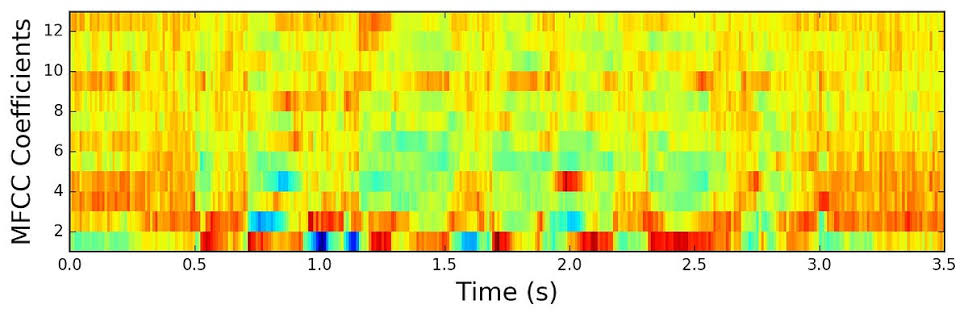
\includegraphics[width=0.85\textwidth]{../assets/figures/ch05-mfcc-matrix.png}}
  \caption{نمایش ماتریسی \eng{MFCC}: محور افقی زمان، محور عمودی شمارهٔ ضریب (۱ تا ۱۳) و رنگ مقدار هر ضریب در هر فریم است. \textit{(برگرفته از تختهٔ کلاس)}}
  \label{fig:mfccmat}
\end{figure}

\begin{exambox}{جمع‌بندی سه مسئله و راه‌حل در تخته}
\begin{enumerate}
  \item \textbf{بانک فیلتر مل}: ادراک غیرخطی فرکانس $\Leftarrow$ مقیاس مل.
  \item \textbf{لگاریتم}: ادراک غیرخطی بلندی (۱۰۰ برابر بلندتر را فقط چند برابر بلندتر حس می‌کنیم) $\Leftarrow$ لگاریتم انرژی مل.
  \item \textbf{\eng{DCT}}: ۴۰ عدد شبیه و تکراری $\Leftarrow$ \eng{DCT} و برداشتن ۱۲ تا ۱۳ ضریب اول.
\end{enumerate}
\end{exambox}

%====================================================================
\section{کاربردهای MFCC}
%====================================================================

ماتریس \eng{MFCC} (برای هر فریم یک بردار ضریب) جایگزین نمایش‌های حجیم‌تر سیگنال می‌شود. کاربردهای مطرح‌شده در کلاس:
\begin{itemize}
  \item \textbf{مقایسهٔ سیگنال‌ها}: استخراج \eng{MFCC} دو سیگنال و سنجش شباهت (مثلاً با هم‌بستگی).
  \item \textbf{تحلیل صدای سرفه}: مقایسهٔ سرفهٔ افراد مبتلا به یک بیماری تنفسی (مانند کووید-۱۹) با سایرین و آموزش یک طبقه‌بند؛ نشان می‌دهد \eng{MFCC} فقط برای تشخیص کلمات نیست.
  \item \textbf{تبدیل گفتار به متن}: به‌جای موج خام، ویژگی‌های آکوستیکی مانند \eng{MFCC} به مدل داده می‌شود؛ ویژگی‌های دیگر (مثل \eng{pitch}) در صورت نیاز جداگانه استخراج می‌شوند.
\end{itemize}

\begin{warningbox}{هشدار}
استخراج \eng{MFCC} یا مشاهدهٔ یک هم‌بستگی به‌تنهایی برای تشخیص بیماری کافی نیست؛ داده‌های معتبر، آموزش و ارزیابی مدل لازم است. مقایسهٔ مستقیم \eng{MFCC} سیگنال‌هایی با طول یا سرعت متفاوت هم به هم‌ترازسازی زمانی (مثلاً \eng{DTW}) یا خلاصه‌سازی آماری نیاز دارد.
\end{warningbox}

%====================================================================
\section{MFCC در یادگیری ماشین و یادگیری عمیق}
%====================================================================

\begin{itemize}
  \item \textbf{آیا استخراج \eng{MFCC} یادگیری ماشین است؟} استاد تأکید کرد خیر: مجموعه‌ای از عملیات ثابت پردازش سیگنال (طیف، بانک فیلتر، لگاریتم، \eng{DCT}، انتخاب ضرایب) با پارامترهای مشخص است و به آموزش روی داده نیاز ندارد؛ اما خروجی‌اش را می‌توان به یک مدل یادگیری ماشین داد.
  \item \textbf{مقایسه با \eng{PCA}} (پرسش دانشجو): از نظر هدف (نمایش فشرده) شبیه‌اند، اما \eng{MFCC} زنجیرهٔ ثابت تبدیل‌هاست و \eng{PCA} روشی آماری است که مؤلفه‌ها را از داده می‌آموزد. اگر پس از لگاریتم مل از \eng{PCA} استفاده شود، دیگر با تعریف متداول \eng{MFCC} کار نمی‌کنیم.
  \item \textbf{در یادگیری عمیق}: می‌توان \eng{MFCC} را هم به مدل داد، چون نمایشی ساختاریافته و فشرده است؛ انتخاب میان موج خام، طیف و \eng{MFCC} به مسئله و عملکرد تجربی بستگی دارد.
\end{itemize}

\begin{correctionbox}{روند امروز: \eng{log-mel} به‌جای \eng{MFCC}}
مدل‌های عصبی امروزی (مانند \eng{Whisper}) بیشتر از لگاریتم انرژی‌های مل (\eng{log-mel}) استفاده می‌کنند و \eng{DCT} را حذف می‌کنند، چون شبکه خودش هم‌بستگی‌ها را می‌آموزد و \eng{DCT} ترتیب فرکانسی را به هم می‌زند. برخی مدل‌ها (مانند \eng{wav2vec 2.0}) از موج خام شروع می‌کنند. \eng{MFCC} همچنان در مدل‌های کلاسیک (\eng{GMM-HMM})، مدل‌های سبک و داده‌های کم کاربرد دارد.
\end{correctionbox}

%====================================================================
\section{جمع‌بندی}
%====================================================================

گوش هم فرکانس را غیرخطی درک می‌کند (نقشهٔ تونوتوپیک، تفکیک بیشتر در بم) و هم شدت را. برای اولی از مقیاس مل و بانک فیلتر مثلثی هم‌پوشان با عرض‌های رشدیابنده و برای دومی از لگاریتم استفاده کردیم. چون ۴۰ انرژی لگاریتمی مل بسیار هم‌بسته‌اند، با \eng{DCT} به ضرایب کپسترال تبدیل شدند و ۱۲ تا ۱۳ ضریب اول نگه داشته شد:
\[
\text{\lr{Speech Signal}}\to\text{\lr{Spectrum}}\to\text{\lr{Mel Filters}}\to\log\to\text{\lr{DCT}}\to\text{\lr{MFCC}} .
\]
نتیجهٔ اصلی: به‌جای همهٔ اطلاعات طیفی، نمایشی فشرده و مناسب گفتار می‌سازیم که ویژگی‌های ادراکی گوش در طراحی آن لحاظ شده است.

\begin{exambox}{نکات مهم برای مرور و امتحان}
\begin{enumerate}
  \item تفاوت $F_0$ با \eng{Pitch} و تفاوت شدت فیزیکی با بلندی ادراک‌شده را بدانید.
  \item نقشهٔ تونوتوپیک (قاعده $\Leftrightarrow$ فرکانس بالا، رأس $\Leftrightarrow$ فرکانس پایین) و پیامد آن (کم‌شنوایی فرکانس بالا با سن) را بشناسید.
  \item توضیح دهید چرا ادراک فرکانس خطی نیست (۱۰۰ تا ۲۰۰ در برابر ۵۱۰۰ تا ۵۲۰۰ هرتز)؛ فرمول $m=2595\log_{10}(1+f/700)$.
  \item بدانید چرا عرض فیلترهای مل در فرکانس‌های بالا بیشتر می‌شود، و هم‌پوشانی و وزن‌دهی مثلثی را توضیح دهید؛ خروجی یک فیلتر را حساب کنید (مثال $M_1=13$).
  \item دلیل لگاریتم از انرژی فیلترها را توضیح دهید.
  \item نقش \eng{DCT} (کاهش هم‌بستگی و فشرده‌سازی) و دلیل نگه‌داشتن ۱۲ یا ۱۳ ضریب را بدانید؛ تعداد فیلترها (حدود ۴۰) و ضرایب ابرپارامترند، نه اجباری.
  \item مسیر استخراج \eng{MFCC} را از سیگنال تا ضرایب نهایی شرح دهید.
  \item \eng{MFCC} (زنجیرهٔ ثابت پردازش سیگنال) را با \eng{PCA} (یادگیری از داده) مقایسه کنید.
  \item معنای واژهٔ کپستروم (جابه‌جایی حروف \eng{Spectrum}، «طیفِ طیف») را بدانید.
\end{enumerate}
\end{exambox}

\chapter{پروسودی و ویژگی‌های زبرزنجیری گفتار}

در جلسات پیشین گفتار را از دید «چه گفته شد؟» بررسی کردیم: واج‌ها، فرمنت‌ها و \eng{MFCC}. این جلسه به پرسش مکمل می‌پردازد: «چگونه گفته شد؟». دو گوینده می‌توانند دقیقاً یک دنبالهٔ واجی را بگویند، اما یکی آن را خبری و دیگری پرسشی، با اطمینان یا با تردید، سریع یا آهسته ادا کند. این لایهٔ دوم را \term{پروسودی}{Prosody} می‌نامیم.

%==========================================================
\section{مرور کوتاه جلسهٔ قبل}
%==========================================================

\textbf{مراحل \eng{MFCC}} روی هر قاب کوتاه: تبدیل فوریه و طیف توان $\leftarrow$ بانک فیلتر مل $\leftarrow$ لگاریتم انرژی هر فیلتر $\leftarrow$ \eng{DCT} $\leftarrow$ نگه‌داشتن چند ضریب نخست (مثلاً ۱۲). فیلترهای مل در فرکانس‌های پایین باریک و در فرکانس‌های بالا پهن‌ترند. تعداد خروجی‌های بانک فیلتر برابر تعداد فیلترهاست (مثلاً ۴۰)، ولی تعداد ضرایب نگه‌داشته‌شده (مثلاً ۱۲) انتخاب جداگانهٔ طراح است؛ این دو الزاماً برابر نیستند.

\begin{correctionbox}{گام چهارم \eng{MFCC} تبدیل فوریهٔ دوباره نیست}
در توضیح شفاهی کلاس از «تبدیل مجدد» سخن رفت. در روش استاندارد، این گام \term{تبدیل کسینوسی گسسته}{DCT} است که روی لگاریتم انرژی‌های بانک فیلتر اعمال می‌شود و ضرایبی کم‌هم‌بسته‌تر می‌دهد.
\end{correctionbox}

\textbf{\eng{MFCC} و مدل منبع–فیلتر.} در مدل \term{منبع–فیلتر}{Source--Filter}، منبع (برای گفتار واک‌دار) ارتعاش تارهای صوتی با فرکانس پایهٔ \eng{$F_0$} است و فیلتر \emph{کل} مجرای صوتی از حنجره تا لب (نه فقط دهان، فک و دندان). \eng{MFCC} عمدتاً شکل طیفی و ویژگی‌های فیلتر را نگه می‌دارد و اطلاعات دقیق منبع، مثل \eng{$F_0$} و زیر و بمی، در آن تضعیف یا حذف می‌شود؛ زیرا فیلترهای مل ساختار هارمونیک را هموار می‌کنند و ضرایب نخست فقط پوش کند طیف را نگه می‌دارند. پس \eng{MFCC} برای تشخیص واج و طبقه‌بندی مناسب است (مثلاً طبقه‌بندی صدای سالم و بیمار، یا ورودی \eng{CNN})، اما برای مطالعهٔ آهنگ جمله کافی نیست؛ این انگیزهٔ بحث پروسودی است.

\textbf{مرور «آ» و «اَ».} تفاوت این دو واکه مربوط به \textbf{فیلتر} است، نه منبع: هر دو واک‌دارند و منبع یکسانی دارند، ولی موقعیت زبان فرق می‌کند و فرمنت‌ها جابه‌جا می‌شوند. هر دو زبان پایینی‌اند (\eng{$F_1$} نسبتاً بالا)، اما «آ» عقبی است و «اَ» جلویی، پس \eng{$F_2$} در «اَ» بالاتر است.

\begin{exambox}{نکتهٔ امتحانی}
هرچه زبان پایین‌تر باشد \eng{$F_1$} بالاتر است؛ هرچه زبان جلوتر باشد \eng{$F_2$} بالاتر است. باید بتوانید با \eng{$F_1$} و \eng{$F_2$} دربارهٔ ارتفاع و موقعیت افقی زبان در تولید واکه‌ها توضیح بدهید.
\end{exambox}

%==========================================================
\section{پروسودی چیست؟}
%==========================================================

\begin{definitionbox}{پروسودی (نوای گفتار)}
\term{پروسودی}{Prosody} مجموعهٔ ویژگی‌هایی از گفتار است که روی دنبالهٔ آواها و واژه‌ها «سوار» می‌شوند و به آن‌ها آهنگ، ریتم، تکیه و الگوی زمانی می‌دهند. پروسودی نشان می‌دهد \textbf{چگونه} گفته شده است، نه فقط \textbf{چه} گفته شده است.
\end{definitionbox}

مثال: «رفتی.» (خبری)، «رفتی؟» (پرسشی) و «رفتی!» (تعجب): واج‌ها یکسان، اما معنا و نیت گوینده متفاوت است. علائم نگارشی بخشی از این اطلاعات را در متن نشان می‌دهند، ولی تصویر کامل پروسودی در متن نیست و باید سیگنال صوتی را تحلیل کرد.

\textbf{قیاس با عروض.} استاد برای نشان دادن «لایه‌ای» بودن پروسودی به عروض اشاره کرد: شعر علاوه بر واژه و معنا روی یک الگوی وزنی (هجاهای کوتاه و بلند) سوار است، مثلاً «به نام خداوند جان و خرد» با الگوی «فعولن فعولن فعولن فعل». برای تحلیل وزن، معنای واژه‌ها اهمیتی ندارد؛ دو عبارت با معنای کاملاً متفاوت می‌توانند وزن یکسان داشته باشند. در گفتار عادی هم واج‌ها یک لایه‌اند و نحوهٔ بیان آن‌ها لایهٔ دیگر. (درس وارد تقطیع شعر نمی‌شود؛ این فقط یک قیاس است.)

\subsection{ویژگی‌های زبرزنجیری}
پروسودی را \term{ویژگی‌های زبرزنجیری}{Suprasegmental Features} هم می‌نامند: «فراتر از قطعه (واج)»؛ مثل چتری که روی قطعات گسترده است. دو پیامد:
\begin{itemize}
  \item تحلیل در سطح چند هجا، عبارت یا کل جمله انجام می‌شود، نه در پنجره‌های ۲۵ میلی‌ثانیه‌ای یا یک واج.
  \item آنچه اهمیت دارد افت و خیزها \emph{نسبت به بخش‌های قبل و بعد} است، نه مقدار مطلق در یک لحظه. از این رو مفهوم \term{کانتور}{Contour} (تغییرات یک ویژگی در طول زمان) محوری است.
\end{itemize}

\subsection{سه مؤلفهٔ اصلی}
«عصبانیت» یا «تردید» خودشان کمیت صوتی نیستند؛ باید ببینیم چه چیزهایی در سیگنال تغییر کرده که شنونده آن را چنین درک می‌کند. این کمیت‌ها در سه گروه جای می‌گیرند: فرکانس، شدت و زمان.

\begin{figure}[htbp]
\centering
\resizebox{\textwidth}{!}{%
\begin{tikzpicture}[rtl, font=\small,
  nd/.style={draw, rounded corners=6pt, align=center, text width=3.1cm, inner sep=5pt, line width=0.6pt},
  note/.style={align=center, text width=5.2cm, font=\footnotesize, text=black!70},
  arr/.style={-{Stealth[length=2.4mm]}, thick, mainblue},
  sk/.style={red!75!black, thick, -{Stealth[length=2mm]}}]
% centre
\node[draw, diamond, aspect=2.2, fill=softred, align=center, inner sep=2pt, line width=0.6pt] (sup) at (0,0) {\lr{suprasegmental}\\\lr{phonetic features}};
\node[note] (supn) at (0,2.9) {\lr{Supra}: فراتر؛ \lr{Segment}: قطعه (بخش). چتری که از بالا روی قطعات گسترده شده است؛ تحلیل در سطح کل جمله یا عبارت، نه فقط یک پنجره یا یک واج؛ افت و خیزها نسبت به بخش قبل و بعد.};
% duration
\node[nd, fill=yellow!30] (dur) at (-6.8,0) {\textbf{\lr{Duration}}\\زمان\\ریتم / مکث\\\lr{punctuation} (کاما)\\\lr{phrasing}\\رفع ابهام نحوی\\تعداد هجا در ثانیه\\کشیده‌شدن};
% intensity
\node[nd, fill=green!20] (int) at (6.3,0) {\textbf{\lr{intensity contour}}\\\lr{energy}\\شدت\\بلندی\\\lr{emphasis}};
\node[note, text width=5cm, font=\small] at (6.3,2.0) {\lr{$\text{Intensity}\propto\text{Magnitude}^{2}$}};
% pitch
\node[nd, fill=cyan!20] (pit) at (0,-3.4) {\textbf{\lr{Pitch Contour}}\\فرکانس\\زیر و بمی\\آهنگ کلام\\\lr{intonation}};
% pitch children
\node[nd, fill=cyan!20, text width=3.4cm] (dec) at (-3.1,-8.2) {کانتور پیچ جمله خبری: زیر و بمی صدا در آخر به سمت بم شدن می‌رود (سقوط فرکانس). نشان‌دهندهٔ قطعیت و پایان است.};
\node[nd, fill=cyan!20, text width=3.4cm] (que) at (0.9,-8.2) {کانتور پیچ جمله سؤالی: بعد از اکسنت، تارهای صوتی کشیده‌تر شده و فرکانس به شدت بالا (زیر) می‌رود («رفتی؟»).};
% intensity children
\node[nd, fill=green!20, text width=3.1cm] (str) at (4.4,-4.6) {\textbf{\lr{stress}}\\یک هجا در درون یک کلمه\\مثل: «مَردی» [اسم مصدر] در برابر «مردی» [یک مرد]};
\node[nd, fill=green!20, text width=3.4cm] (acc) at (8.4,-4.6) {\textbf{\lr{Accent/Focus}}\\یک کلمه در درون یک جمله\\کانتور اینتنسیتی: اکسنت = قله؛ سکوت یا گفتار بی‌تأکید = صاف};
\node[note, text width=4.2cm] (accn) at (8.4,-8.9) {کلمات در فرهنگ لغت و برای لهجهٔ خاص، استرس مشخصی دارند؛ اما این گوینده است که در موقعیت‌های مختلف تصمیم می‌گیرد به کدام کلمه در گفتمان (\lr{Discourse}) اکسنت بدهد.};
% arrows
\draw[arr] (sup.west) -- (dur.east);
\draw[arr] (sup.east) -- (int.west);
\draw[arr] (sup.south) -- (pit.north);
\draw[arr] (pit.south) -- ++(0,-0.4) -| (dec.north);
\draw[arr] (pit.south) -- ++(0,-0.4) -| (que.north);
\draw[arr] (int.south) -- ++(0,-0.4) -| (str.north);
\draw[arr] (int.south) -- ++(0,-0.4) -| (acc.north);
\draw[densely dashed, black!50] (acc.south) -- (accn.north);
% red sketches: fall / rise
\draw[sk] ([xshift=-0.9cm,yshift=-0.2cm]dec.south) -- ++(0.7,-0.8);
\node[red!75!black, font=\footnotesize] at ([xshift=0.8cm,yshift=-0.55cm]dec.south) {افت};
\draw[sk] ([xshift=-0.9cm,yshift=-0.2cm]que.south) to[out=-80,in=180] ++(0.4,-0.7) to[out=0,in=-110] ++(0.8,0.35);
\node[red!75!black, font=\footnotesize] at ([xshift=0.9cm,yshift=-0.55cm]que.south) {خیز};
\end{tikzpicture}}
\caption{نقشهٔ ذهنی ویژگی‌های زبرزنجیری: سه شاخهٔ زمان (\eng{Duration})، زیر و بمی (\eng{Pitch Contour}) و شدت (\eng{Intensity Contour}). شاخهٔ شدت به تکیهٔ واژگانی (\eng{stress}) و تأکید (\eng{Accent/Focus}) تقسیم شده است؛ شاخهٔ زیر و بمی به کانتور جملهٔ خبری و پرسشی. (بازسازی‌شده از تختهٔ کلاس)}
\end{figure}

\begin{table}[htbp]
\centering
\caption{سه مؤلفهٔ اصلی پروسودی، کمیت فیزیکی و ادراک متناظر. (جدول افزوده)}
\begin{tabular}{p{2.3cm}p{3.4cm}p{3.4cm}p{4.2cm}}
\toprule
مؤلفه & کمیت فیزیکی & ادراک شنونده & واحد/ابزار \\
\midrule
فرکانس & فرکانس پایه \eng{($F_0$)} & زیر و بمی (\eng{Pitch}) & هرتز، نیم‌پرده؛ کانتور \eng{$F_0$} \\
شدت & دامنه، انرژی & بلندی (\eng{Loudness}) & دسی‌بل؛ کانتور شدت \\
زمان & مدت آوا/هجا، مکث & سرعت، ریتم، کشش & میلی‌ثانیه، هجا در ثانیه \\
\bottomrule
\end{tabular}
\end{table}

%==========================================================
\section{مؤلفهٔ اول: شدت صدا}
%==========================================================

\subsection{شدت و دسی‌بل}
اصطلاحات \eng{Intensity}، \eng{Energy}، \eng{Loudness}، \eng{Amplitude} و \eng{Magnitude} از نظر علمی دقیقاً هم‌معنا نیستند، ولی در این جلسه در یک گروه قرار گرفته‌اند. رابطهٔ تخته: شدت با مربع دامنه متناسب است، $\text{\lr{Intensity}}\propto\text{\lr{Magnitude}}^{2}$. بلندی (\eng{Loudness}) کمیتی \textbf{ادراکی} است و با شدت فیزیکی یکی نیست. چون انسان نسبت‌های شدت را حس می‌کند و بازهٔ شدت‌های شنیدنی بسیار گسترده است، از مقیاس لگاریتمی \term{دسی‌بل}{dB} استفاده می‌شود.

\begin{definitionbox}{تراز شدت و تراز فشار صوت}
\begin{align*}
L_I &= 10\log_{10}\!\left(\frac{I}{I_0}\right)\ \text{dB}, \qquad I_0=10^{-12}\ \text{W/m}^2 \\
L_p &= \text{\lr{SPL}} = 20\log_{10}\!\left(\frac{p}{p_0}\right)\ \text{dB}, \qquad p_0=20\ \mu\text{Pa}
\end{align*}
چون $I\propto p^2$، ضریب لگاریتم برای دامنه ۲۰ و برای توان یا شدت ۱۰ است.
\end{definitionbox}

مثال‌ها: دو برابر شدن \textbf{دامنه} برابر $20\log_{10}2\approx+6\,\text{dB}$ است (نصف شدن: $-6\,\text{dB}$)؛ دو برابر شدن \textbf{توان} برابر $+3\,\text{dB}$؛ ده برابر شدن دامنه برابر $+20\,\text{dB}$. فشار $p=0{,}02\,\text{Pa}$ معادل $20\log_{10}(1000)=60\,\text{dB SPL}$ و در حد گفت‌وگوی معمولی است.

\coursefigure{0.85}{ch06-db-amplitude.png}{سمت چپ: یک تن خالص با دامنه‌های ۱، ۲ و ۱۰. سمت راست: رابطهٔ لگاریتمی دسی‌بل با نسبت دامنه؛ دو برابر شدن دامنه حدود $+6$ دسی‌بل و ده برابر شدن آن $+20$ دسی‌بل است. (شکل افزوده)}

\textbf{کانتور شدت:} برای هر قاب (مثلاً ۲۵ میلی‌ثانیه، گام ۱۰ میلی‌ثانیه) انرژی میانگین $E=\frac1N\sum_n x^2[n]$ را حساب و $10\log_{10}(E+\varepsilon)$ را در طول زمان رسم می‌کنیم.

\begin{correctionbox}{بلندی با شدت یکی نیست}
بلندی ادراک‌شده تابع شدت، فرکانس و مدت صوت است: دو صدا با شدت یکسان ولی فرکانس متفاوت بلندی یکسان ندارند و گوش در حدود ۲ تا ۵ کیلوهرتز حساس‌ترین است. قاعدهٔ سرانگشتی: حدود ۱۰ دسی‌بل افزایش، بلندی را تقریباً دو برابر می‌کند.
\end{correctionbox}

\subsection{تکیهٔ واژگانی و تأکید}

\begin{definitionbox}{\eng{Stress} در برابر \eng{Accent}}
\textbf{تکیهٔ واژگانی} (\eng{Lexical Stress}): برجستگی یک \textbf{هجا درون یک واژه}؛ بخشی از الگوی تلفظ واژه و وابسته به زبان و لهجه.

\textbf{تأکید} (\eng{Accent/Focus}): برجسته‌کردن یک \textbf{واژه درون جمله}؛ گوینده بر اساس قصد و بافت تصمیم می‌گیرد کدام واژه را برجسته کند. در کانتور شدت، تأکید به‌صورت یک \textbf{قله} دیده می‌شود و گفتار بی‌تأکید یا سکوت تقریباً صاف است.
\end{definitionbox}

مثال‌های کلاس: در «من گفتم که این کار را بکن» تأکید روی «من» است و در «کتاب را بردار» روی «کتاب».

\begin{warningbox}{«اکسنت» دو معنا دارد}
در این درس \eng{accent} یعنی «تأکید روی یک واژه در جمله»، نه «لهجه» (مثل لهجهٔ شیرازی)؛ و \eng{stress} یعنی «تکیه»، نه «استرس روانی».
\end{warningbox}

\textbf{رابطهٔ \eng{Accent} با \eng{Stress}} (نکته‌ای که استاد چند بار تکرار کرد): هنگام تأکید روی یک واژه، برجستگی روی همان هجایی قرار می‌گیرد که تکیهٔ واژگانی دارد؛ تأکید محل تکیه را عوض نمی‌کند و فقط برجستگی هجای تکیه‌دار را تقویت می‌کند. («نمی‌توان روی هجایی اکسنت گذاشت که استرس ندارد.») این ایده با \term{شبکهٔ متریک}{Metrical Grid} نمایش داده می‌شود؛ استاد گفت این مبحث بیشتر مربوط به تحلیل‌های زبان‌شناختی است و در درس کاربرد تخصصی ندارد.

\begin{correctionbox}{نشانگرهای تأکید فقط شدت نیستند}
کلاس تأکید را در شاخهٔ «شدت» جای داد و با قله در کانتور شدت شناخت؛ این درست ولی ناقص است. در پژوهش‌های آوایی، نشانگرهای تکیه و تأکید ترکیبی‌اند: تغییر \eng{$F_0$}، افزایش مدت هجا و کامل‌تر ادا شدن واکه، و سپس شدت (که در بسیاری از آزمایش‌ها ضعیف‌ترین نشانهٔ مستقل است). پس باید کانتور شدت، \eng{$F_0$} و مدت را هم‌زمان بررسی کرد.
\end{correctionbox}

\coursefigure{0.85}{ch06-synthetic-intensity.png}{کانتور شدت برای جملهٔ «کتاب را به علی دادی» در خوانش خنثی (خاکستری) و در حالتی که روی «علی» تأکید شده است (سبز): تأکید به‌صورت قله روی هجای تکیه‌دار آن واژه دیده می‌شود. داده‌ها مصنوعی و فقط برای توضیح مفهوم‌اند. (شکل افزوده)}

\begin{assignmentbox}{تمرین پیشنهادی با \eng{Praat}}
یک واژه یا جمله را یک بار عادی و یک بار با تأکید یا لحن عصبانی ضبط کنید و کانتور شدت و کانتور \eng{$F_0$} را مقایسه کنید. بررسی کنید که افزایش شدت و کشش در همان هجای تکیه‌دار رخ می‌دهد یا نه، و محل تکیه تغییر می‌کند یا نه.
\end{assignmentbox}

%==========================================================
\section{مؤلفهٔ دوم: فرکانس و زیر و بمی}
%==========================================================

\subsection{\eng{$F_0$}، \eng{Pitch} و آهنگ}
\begin{itemize}
  \item \term{فرکانس پایه}{\eng{$F_0$}}: کمیتی \textbf{فیزیکی}؛ تعداد دورهٔ ارتعاش تارهای صوتی در ثانیه (هرتز).
  \item \term{زیر و بمی}{Pitch}: کمیتی \textbf{ادراکی}؛ آنچه شنونده «زیر» یا «بم» می‌شنود. در عمل با \eng{$F_0$} یکی گرفته می‌شود.
  \item \term{کانتور زیر و بمی}{Pitch Contour}: تغییر \eng{$F_0$} در طول یک جمله یا عبارت.
  \item \term{آهنگ جمله}{Intonation}: الگوی منظم و معنادار این تغییرات که نقش زبانی دارد (مثلاً تمایز خبر و پرسش).
\end{itemize}

\begin{addedbox}{نیم‌پرده}
شنوایی زیر و بمی را تقریباً لگاریتمی حس می‌کند؛ پس برای مقایسه از \term{نیم‌پرده}{Semitone} استفاده می‌شود: $\Delta=12\log_2(f_2/f_1)$. مثلاً ۲۰۰ تا ۴۰۰ هرتز دقیقاً ۱۲ نیم‌پرده (یک اکتاو) است و ۲۰۰ تا ۲۵۰ هرتز حدود $3{,}9$ نیم‌پرده. همچنین \eng{$F_0$} فقط در قطعات واک‌دار تعریف می‌شود، پس کانتور در بی‌واک‌ها «پاره» است.
\end{addedbox}

\subsection{کانتور جملهٔ خبری و پرسشی}
\begin{itemize}
  \item \textbf{جملهٔ خبری}: زیر و بمی در پایان به سمت بم‌شدن می‌رود (سقوط فرکانس)؛ نشان‌دهندهٔ \textbf{قطعیت و پایان}.
  \item \textbf{جملهٔ پرسشی}: بعد از اکسنت، تارهای صوتی کشیده‌تر می‌شوند و فرکانس به شدت بالا می‌رود (مثال: «رفتی؟»).
\end{itemize}

\boardfigure{0.95}{ch06-board-metrical-grid.png}{کانتور \eng{$F_0$} نرمال‌شده (برحسب هرتز) در طول زمان نرمال‌شده برای چهار حالت \eng{Statement}، \eng{Question}، \eng{Happy} و \eng{Sad}. جملهٔ خبری در پایان افت می‌کند، پرسشی در پایان بالا می‌رود، حالت شاد در سطح بالاتر و تقریباً هموار است و حالت غمگین ابتدا بالا و سپس با افت شدید تمام می‌شود. دو منحنی رنگی با نوارهای اطمینان خاکستری دو گروه یا شرایط را نشان می‌دهند؛ تعریف آن‌ها در اسلاید ذکر نشده است.}

\begin{correctionbox}{«خبری = افت، پرسشی = خیز» گرایش است، نه قانون}
خیز پایانی در پرسش‌های بله/خیر رایج است، ولی پرسش‌های دارای واژهٔ پرسشی (چرا، کجا، چه) اغلب افتان‌اند. در فارسی گفتاری، پرسش بله/خیر اغلب فقط با آهنگ ساخته می‌شود («رفتی؟» در برابر «رفتی.»). شکل دقیق کانتور به گوینده، زبان و تأکید هم بستگی دارد. فارسی تونال نیست (برخلاف ماندارین که زیر و بمی در سطح واژه معنا می‌سازد).
\end{correctionbox}

\textbf{مثال «کتاب را به علی دادی؟»:} استاد این جمله را چند بار با لحن‌های گوناگون گفت: در حالت پرسشی \eng{$F_0$} در پایان بالا می‌رود و در حالت خبری پایین می‌آید. یک بار خیز پایانی به اندازهٔ انتظار روشن نبود؛ یعنی یک الگوی پروسودیک همیشه یک‌شکل تولید نمی‌شود و باید نمونه‌های زیادی را بررسی کرد. اگر روی «علی» تأکید شود، علاوه بر شدت، کانتور \eng{$F_0$} هم در آن ناحیه تغییر محسوسی دارد؛ پس بهتر است کانتور شدت و زیر و بمی را هم‌زمان بررسی کنیم.

\textbf{جمله‌های دستوری و احساسی:} در دستور قاطع ممکن است افت پایانی شدیدتر از جملهٔ خبری معمولی باشد؛ در درخواست مؤدبانه («بفرمایید، بشینید.») الگو متفاوت و لحن ملایم‌تر است؛ و شادی و غم کانتور و سطح متفاوتی دارند (شکل بالا). الگوی زیر و بمی به شیوهٔ بیان و قصد ارتباطی هم وابسته است، نه فقط کلمات.

%==========================================================
\section{مؤلفهٔ سوم: زمان، ریتم و مکث}
%==========================================================

\begin{table}[htbp]
\centering
\caption{ویژگی‌های زمانی گفتار (شاخهٔ \eng{Duration} در نقشهٔ کلاس).}
\begin{tabular}{p{3.3cm}p{9.5cm}}
\toprule
ویژگی & توضیح \\
\midrule
\eng{Duration} & مدت‌زمان بیان یک آوا، هجا، واژه یا عبارت \\
\eng{Speech Rate} & سرعت گفتار؛ ساده‌ترین معیار «تعداد هجا در ثانیه» است \\
\eng{Rhythm} & الگوی زمانی و ریتمیک گفتار \\
\eng{Pause} & مکث و سکوت \\
\eng{Lengthening} & کشیده‌شدن آواها \\
\eng{Phrasing} & تقسیم گفتار به گروه‌ها و عبارت‌های آهنگین \\
\bottomrule
\end{tabular}
\end{table}

\begin{addedbox}{سرعت گفتار در برابر سرعت تلفظ}
\term{سرعت گفتار}{Speech Rate} مکث‌ها را در زمان کل حساب می‌کند و \term{سرعت تلفظ}{Articulation Rate} فقط زمان گفتار واقعی را. مثلاً اگر ۱۹ هجا در $4{,}5$ ثانیه ادا شود که $0{,}5$ ثانیه آن مکث است: $19/4{,}5\approx 4{,}2$ هجا در ثانیه (گفتار) در برابر $19/4\approx 4{,}75$ (تلفظ).
\end{addedbox}

\textbf{مکث و علائم نگارشی.} مکث می‌تواند معنای نحوی جمله را تغییر دهد و مرز دو عبارت را روشن کند. ویرگول، دونقطه و نقطه نشانهٔ محل مکث یا بخش‌بندی‌اند؛ ولی همهٔ علائم زمانی نیستند (علامت سؤال به آهنگ مربوط است).

\textbf{رفع ابهام نحوی.} گاهی جمله در متن بیش از یک تفسیر دارد، اما در گفتار محل مکث‌ها، کشش آواها و گروه‌بندی زمانی ساختار مورد نظر را نشان می‌دهد (\term{رفع ابهام نحوی}{Syntactic Disambiguation}). مثلاً «مردان و زنان باهوش» (مثال افزوده، نه از کلاس): مکث پس از «مردان» یعنی «(مردان) و (زنان باهوش)» و مکث پس از «زنان» یعنی «(مردان و زنان) باهوش».

\coursefigure{0.85}{ch06-pause-phrasing.png}{دو گروه‌بندی ممکن برای «مردان و زنان باهوش» که فقط در جای مکث تفاوت دارند. مدت‌ها فرضی و برای توضیح‌اند. (شکل افزوده)}

%==========================================================
\section{پروسودی در تبدیل متن به گفتار}
%==========================================================

استاد چند نمونه خروجی از یک سامانهٔ فارسی تبدیل متن به گفتار پخش کرد. در نمونهٔ اول («مادر کتاب را روی میز اتاق گذاشت و پنجره را باز کرد.») مکث و گروه‌بندی طبیعی نبود: مدل واج‌ها را ساخته بود اما پروسودی مناسب جمله را بازسازی نکرده بود. در نمونهٔ دوم (جمله‌ای دربارهٔ شرکت \eng{Anthropic}) کسرهٔ اضافه نامناسب تولید می‌شد و سرعت گفتار نسبتاً بالا بود. (استاد از داده‌های آموزشی آن سامانه مطمئن نبود، پس نتیجهٔ قطعی دربارهٔ شیوهٔ آموزش آن نمی‌توان گرفت.)

کیفیت \eng{TTS} فقط به تلفظ درست واج‌ها وابسته نیست؛ سامانه باید محل مکث‌ها، طول هجاها، ریتم، الگوی تأکید، اتصال طبیعی واژه‌ها (مثل کسرهٔ اضافه) و آهنگ را هم درست تولید کند. دلیل دشواری: نگاشت متن به پروسودی «یک‌به‌چند» است و قصد گوینده و احساس در متن نیامده‌اند.

%==========================================================
\section{پژوهش: اطمینان و صداقت ادراک‌شده از روی پروسودی}
%==========================================================

\begin{assignmentbox}{تمرین طراحی آزمایش}
آزمایشی طراحی کنید که نشان دهد صداقت و اطمینان یک گوینده، در نحوهٔ بیان او و ویژگی‌های پروسودیک گفتارش، الگوهای مشترکی دارند.
\end{assignmentbox}

نکتهٔ مهم: باید میان (۱) اطمینان یا صداقتی که \textbf{شنونده} از صدا \emph{برداشت} می‌کند و (۲) اطمینان یا صداقت \textbf{واقعی} گوینده فرق گذاشت. آزمایش ادراکی کلاس موضوع اول را می‌سنجد.

\textbf{فرضیه‌های اولیهٔ کلاس} (قابل آزمون، نه قاعدهٔ قطعی):
\begin{itemize}
  \item \textbf{شدت}: شدت بیشتر یا تأکید واضح‌تر احساس تسلط می‌دهد؛ اما بلندی صدای افراد یکسان نیست، پس ابتدا باید ویژگی‌های معمول هر گوینده را به‌عنوان \term{خط پایه}{Baseline} در نظر گرفت و تغییرات همان فرد را بررسی کرد.
  \item \textbf{زیر و بمی}: افت \eng{$F_0$} در پایان عبارت قطعیت را منتقل می‌کند.
  \item \textbf{زمان و مکث}: مکث‌های متعدد در میانهٔ جمله تردید را می‌رساند؛ اما مکث در ابتدا یا انتها ممکن است متانت را برساند. پس \textbf{محل} مکث هم مهم است.
\end{itemize}

\textbf{طرح آزمایش پیشنهادی:}
\begin{center}
\begin{tikzpicture}[rtl, node distance=0.7cm and 0.9cm, >=Stealth,
  box/.style={draw, rounded corners, align=center, minimum width=2.7cm, minimum height=1.3cm, font=\small, fill=blue!6}]
  \node[box] (a) {\RL{۱. جمع‌آوری گفتار}\\\RL{جملهٔ یکسان با}\\\RL{شیوه‌های بیان متفاوت}};
  \node[box, left=of a] (b) {\RL{۲. ارزیابی شنونده}\\\RL{امتیاز اطمینان و}\\\RL{صداقت ادراک‌شده}};
  \node[box, left=of b] (c) {\RL{۳. استخراج ویژگی}\\\lr{Pitch, Intensity,}\\\lr{Duration}};
  \node[box, left=of c] (d) {\RL{۴. تحلیل آماری}\\\RL{هم‌بستگی ویژگی‌ها}\\\RL{با امتیاز شنوندگان}};
  \draw[->] (a) -- (b); \draw[->] (b) -- (c); \draw[->] (c) -- (d);
\end{tikzpicture}
\end{center}

\begin{definitionbox}{هم‌بستگی (\eng{Correlation})}
\textbf{هم‌بستگی مثبت}: با افزایش یک متغیر، دیگری نیز تمایل به افزایش دارد (مثلاً شدت بیشتر با امتیاز اطمینان بیشتر). \textbf{هم‌بستگی منفی}: دیگری تمایل به کاهش دارد (مثلاً مدت طولانی‌تر با اطمینان کمتر). نزدیک صفر یعنی رابطهٔ خطی ضعیف است. ضریب پیرسون بین $-1$ و $+1$ است و هم‌بستگی به‌تنهایی علیت را ثابت نمی‌کند.
\end{definitionbox}

\subsection{مقالهٔ بررسی‌شده}
مقاله با عنوان
\textit{\lr{Listeners' perceptions of the certainty and honesty of a speaker are associated with a common prosodic signature}}
(\eng{Goupil et al., Nature Communications, 2021}) است. در مطالعهٔ اول طبق گزارش‌ها، شنوندگان بین دو نسخه از یک شبه‌واژه که \eng{$F_0$}، بلندی و مدت آن‌ها تصادفی تغییر کرده بود انتخاب می‌کردند کدام «مطمئن‌تر» یا «صادق‌تر» است، و با \term{هم‌بستگی معکوس}{Reverse Correlation} «هستهٔ پروسودیک» هر قضاوت به دست می‌آمد. (آنچه روی تخته آمد خلاصهٔ آموزشی است؛ جزئیات را از متن مقاله بازبینی کنید.)

\textbf{خواندن نمودارها.} ردیف بالا مربوط به \textbf{اطمینان} (آبی) و ردیف پایین \textbf{صداقت} (سبز) است؛ ستون‌ها \eng{pitch}، \eng{loudness} و \eng{duration}. محور افقی «قطعه» است: بخش‌های زمانی یک محرک کوتاه (۱۲ قطعه برای \eng{$F_0$} و بلندی، ۵ قطعه برای مدت)، نه بخش‌های یک جملهٔ بلند. محور عمودی دامنهٔ هسته؛ خط خطچین صفر یعنی «بدون اثر».

\boardfigure{0.95}{ch06-paper-kernels.png}{هسته‌های پروسودیک اطمینان (ردیف بالا) و صداقت (ردیف پایین) برای \eng{pitch}، \eng{loudness} و \eng{duration} در برابر قطعهٔ زمانی. مقدار مثبت یعنی ویژگی در آن قطعه با انتخاب «مطمئن‌تر/صادق‌تر» همراه بوده؛ منفی یعنی عکس؛ نزدیک صفر یعنی بی‌اثر. (مقاله: \eng{Goupil et al., 2021})}

\begin{table}[htbp]
\centering
\caption{خلاصهٔ الگوهای نمودار.}
\begin{tabular}{p{2.1cm}p{6.1cm}p{5.2cm}}
\toprule
ویژگی & الگوی دیده‌شده & برداشت \\
\midrule
\eng{Pitch} & در ابتدا نزدیک صفر، در نیمهٔ دوم منفی & افت آهنگ در بخش پایانی با اطمینان و صداقت بیشتر همراه است \\
\eng{Loudness} & مثبت در چند قطعه (ابتدایی/میانی) & شدت بیشتر در این بخش‌ها با اطمینان یا صداقت بیشتر همراه است \\
\eng{Duration} & منفی در قطعه‌های میانی، نزدیک صفر در دو سر & طولانی‌تر (کندتر) بودن با اطمینان و صداقت کمتر همراه است \\
\bottomrule
\end{tabular}
\end{table}

نکتهٔ اصلی: اثر هر ویژگی به \textbf{جایگاه زمانی} آن بستگی دارد (مثلاً شدت در ابتدا بی‌اثر و در میانه مؤثر است)، پس میانگین کل جمله کافی نیست.

\begin{correctionbox}{دقت در تفسیر نمودار}
(۱) نمودار مدت به سرعت گفتار مربوط است، نه به «مکث» به معنای سکوت؛ در مقاله سرعت بیشتر (مدت کوتاه‌تر) با اطمینان بیشتر همراه است. (۲) «ابتدا، میانه و انتهای جمله» در کلاس را باید «ابتدا، میانه و انتهای محرک (واژه)» خواند. (۳) ایدهٔ مقاله «شکل» کانتور است؛ «فرکانس پایین‌تر» یعنی افت آهنگ در بخش پایانی، نه صدای بم‌تر به‌طور کلی. (۴) نتیجه دربارهٔ \textbf{برداشت شنونده} است، نه صداقت واقعی، و همبستگی است نه علیت.
\end{correctionbox}

%==========================================================
\section{کاربردهای عملی تحلیل پروسودی}
%==========================================================

یک نمونه که استاد اشاره کرد ارزیابی نحوهٔ بیان افراد در \textbf{مصاحبهٔ شغلی} است. چنین سامانه‌ای می‌تواند ترکیب کند: (۱) \textbf{محتوا} با \eng{ASR}، (۲) \textbf{نحوهٔ بیان} (شدت، فرکانس، سرعت گفتار) و (۳) \textbf{تحلیل چندوجهی} (متن، صدا و گاهی تصویر) برای ارائهٔ امتیاز یا برآورد.

\begin{warningbox}{احتیاط در استفاده}
چنین امتیازهایی لزوماً بیانگر شخصیت، تخصص یا صداقت واقعی فرد نیستند و اعتبار آن‌ها نیازمند ارزیابی مستقل و کنترل تفاوت‌های فردی، زبانی و موقعیتی است.
\end{warningbox}

%==========================================================
\section{جمع‌بندی}
%==========================================================

پروسودی لایه‌ای از گفتار است که «چگونه گفتن» را توصیف می‌کند و تمام آن در متن نیست. سه مؤلفهٔ آن زیر و بمی، شدت و زمان‌اند و باید به‌صورت کانتور روی بازه‌های بلند بررسی شوند؛ تحلیل طیفی به‌تنهایی کافی نیست.

\begin{exambox}{نکات مهم برای مرور و امتحان}
\begin{enumerate}
  \item \eng{MFCC} شکل طیفی و فیلتر مجرا را نشان می‌دهد و اطلاعات \eng{$F_0$} را عملاً حذف می‌کند. تعداد خروجی‌های بانک فیلتر برابر تعداد فیلترهاست و ضرایب نهایی (مثلاً ۱۲) می‌تواند کمتر باشد؛ گام پس از لگاریتم \eng{DCT} است.
  \item اختلاف «آ» و «اَ» مربوط به فیلتر است: زبان پایین‌تر $\Rightarrow$ \eng{$F_1$} بالاتر؛ زبان جلوتر $\Rightarrow$ \eng{$F_2$} بالاتر.
  \item پروسودی (زبرزنجیری) ریتم، آهنگ و تأکید را توصیف می‌کند؛ سه مؤلفه: \eng{Pitch/Frequency}، \eng{Intensity}، \eng{Time/Duration}؛ باید یک عبارت و کانتور آن را بررسی کرد.
  \item \eng{Stress}: تکیه درون واژه؛ \eng{Accent}: برجسته‌سازی واژه در جمله؛ تأکید روی همان هجای تکیه‌دار می‌نشیند.
  \item کانتور شدت ناحیه‌های تأکیدی را نشان می‌دهد، اما \eng{$F_0$} و مدت هم در تأکید نقش دارند. شدت با مربع دامنه متناسب است؛ $L_p=20\log_{10}(p/p_0)$ و $L_I=10\log_{10}(I/I_0)$.
  \item کانتور پرسشی اغلب با خیز و خبری با افت پایانی همراه است (گرایش، نه قانون).
  \item ویژگی‌های زمانی (سرعت گفتار، مدت هجا، ریتم، مکث، کشش) در \eng{Phrasing} و رفع ابهام نحوی نقش دارند.
  \item آزمایش اطمینان/صداقت: جمع‌آوری گفتار، ارزیابی شنونده، استخراج ویژگی، تحلیل هم‌بستگی؛ جایگاه زمانی ویژگی مهم است و باید بتوانید هم‌بستگی مثبت/منفی/نزدیک صفر را در نمودار تفسیر کنید.
\end{enumerate}
\end{exambox}

\chapter{تبدیل متن به گفتار: مسئله و معماری خط‌لولهٔ \eng{TTS}}

\section{از تحلیل گفتار تا تولید گفتار}

تا این جلسه محور درس \textbf{تحلیل سیگنال گفتار} بود: موج صوتی از پیش در اختیار ما بود و از آن طیف‌نگار، \eng{MFCC}، پروزودی، فرمنت‌ها و ... استخراج می‌کردیم. از این جلسه وارد سامانه‌های اصلی می‌شویم: تبدیل متن به گفتار (\eng{TTS})، سامانه‌های گفت‌وگو و تبدیل گفتار به متن (\eng{STT}). موضوع این جلسه \term{تبدیل متن به گفتار}{Speech Synthesis} است. در \eng{TTS} جهت مسئله معکوس می‌شود:
\[
\text{\lr{Text}} \;\longrightarrow\; \text{\lr{Speech Waveform}}
\]
دو مشکل بنیادی وجود دارد:
\begin{itemize}
  \item \textbf{شکاف حجم اطلاعات:} متن بسیار کم‌حجم است (چند ده نویسه یا واج)، اما با نرخ نمونه‌برداری $f_s = 24\,000$ هرتز هر ثانیه گفتار ۲۴ هزار نمونه دارد.
  \item \textbf{کم‌گویی متن:} متن لحن، تأکید، سرعت، مکث و ویژگی‌های گوینده را مشخص نمی‌کند؛ پس مدل باید این‌ها را از داده و بافت \textbf{استنتاج یا تولید} کند. نگاشت متن به گفتار یک‌به‌چند است.
\end{itemize}


\section{دو رویکرد کلی: خط‌لوله و سرتاسری}

\begin{itemize}
  \item \textbf{خط‌لوله‌ای (\eng{Pipeline-Based}):} مسئله به چند ماژول با وظیفهٔ مشخص تقسیم می‌شود و خروجی هر ماژول ورودی بعدی است. هر بخش را می‌توان جداگانه بررسی، آموزش، اصلاح یا جایگزین کرد.
  \item \textbf{سرتاسری (\eng{End-to-End}):} یک مدل (یا مجموعهٔ یکپارچه‌ای از لایه‌ها) متن را مستقیماً به گفتار می‌رساند و لزوماً ماژول‌های میانی مستقل و قابل مشاهده ندارد.
\end{itemize}

\begin{exambox}{نکتهٔ تأکیدی استاد}
رویکرد \eng{End-to-End} \textbf{لزوماً بهترین گزینه برای همهٔ کاربردها نیست}. گاهی به‌دلیل تأخیر پردازش (\eng{Latency}) یا ویژگی‌های دامنهٔ کاربرد (مثلاً حساسیت مرحلهٔ نرمال‌سازی متن)، ماژول‌های کلاسیک یا خط‌لوله مناسب‌ترند. در این جلسه تمرکز بر خط‌لوله است و رویکردهای سرتاسری در جلسهٔ جدا می‌آیند.
\end{exambox}

\begin{correctionbox}{«سرتاسری» یک طیف است}
برخی مدل‌ها (مثل \eng{Tacotron 2}) فقط تا طیف‌نگار سرتاسری‌اند و وکودر جدا دارند؛ مدل‌هایی مانند \eng{VITS} واج را در یک مدل به موج می‌رسانند، و حتی آن‌ها نرمال‌سازی و \eng{G2P} را بیرون از مدل می‌گذارند. پس مسئله بیشتر این است که مرز ماژول‌ها کجا باشد.
\end{correctionbox}

\section{معماری کلی یک سامانهٔ \eng{TTS}}

سامانهٔ \eng{TTS} دو بخش اصلی دارد:
\begin{description}
  \item[\eng{Front-End} (تحلیل متن، \eng{Text Analysis}).] ورودی هنوز متن است؛ «چه باید گفته شود». خروجی: توالی واج‌ها.
  \item[\eng{Back-End} (تولید گفتار، \eng{Speech Synthesis}).] واج‌ها به نمایش آکوستیکی و سپس به موج تبدیل می‌شوند؛ «چگونه گفته شود».
\end{description}

\begin{figure}[!htbp]
\centering
\resizebox{\textwidth}{!}{%
\begin{tikzpicture}[rtl,
  box/.style={draw, rounded corners=3pt, minimum width=2.55cm, minimum height=1.0cm, align=center, fill=softblue, font=\small},
  data/.style={draw, rounded corners=1pt, minimum width=2.2cm, minimum height=0.8cm, align=center, fill=softyellow, font=\small},
  arr/.style={-{Stealth[length=2.5mm]}, thick},
  small/.style={font=\scriptsize, text=black!65, align=center}
]
% Front-end (right to left)
\node[data] (txt) at (12.2,0) {\rl{متن خام}\\\scriptsize\lr{Text}};
\node[box] (norm) at (9.1,0) {\rl{نرمال‌سازی متن}\\\scriptsize\lr{Text Normalization}};
\node[box] (homo) at (6.0,0) {\rl{رفع ابهام هم‌نویسه}\\\scriptsize\lr{Homograph Disamb.}};
\node[box] (g2p) at (2.9,0) {\rl{تبدیل نویسه به واج}\\\scriptsize\lr{G2P}};
\node[data] (ph) at (0,0) {\rl{توالی واج‌ها}\\\scriptsize\lr{Phonemes}};
\draw[arr] (txt) -- (norm);
\draw[arr] (norm) -- (homo);
\draw[arr] (homo) -- (g2p);
\draw[arr] (g2p) -- (ph);
% Back-end (left to right)
\node[box, fill=softgreen] (am) at (3.1,-2.7) {\rl{مدل آکوستیکی}\\\scriptsize\lr{Acoustic Model}};
\node[data] (mel) at (6.1,-2.7) {\rl{طیف‌نگار مل}\\\scriptsize\lr{Mel-Spectrogram}};
\node[box, fill=softgreen] (voc) at (9.1,-2.7) {\rl{وکودر}\\\scriptsize\lr{Vocoder}};
\node[data] (wav) at (12.2,-2.7) {\rl{موج گفتار}\\\scriptsize\lr{Waveform}};
\draw[arr] (ph.south) |- (am.west);
\draw[arr] (am) -- (mel);
\draw[arr] (mel) -- (voc);
\draw[arr] (voc) -- (wav);
% region labels
\draw[dashed, gray] (-1.4,0.95) rectangle (13.5,-0.95);
\node[anchor=south west, font=\small\bfseries, text=mainblue] at (-1.3,0.95) {\lr{Front-End: Text Analysis}};
\draw[dashed, gray] (1.7,-1.75) rectangle (13.5,-4.15);
\node[anchor=north west, font=\small\bfseries, text=mainblue] at (1.8,-4.2) {\lr{Back-End: Speech Generation}};
% size notes
\node[small] at (-0.9,-1.3) {\rl{$30$--$50$ واج}};
\node[small, anchor=north] at (6.1,-3.3) {\rl{$\approx 80$ قاب بر ثانیه}};
\node[small, anchor=north] at (12.2,-3.3) {\rl{$\approx 24000$ نمونه بر ثانیه}};
\end{tikzpicture}}
\caption{نمودار بلوکی خط‌لولهٔ \eng{TTS}: تحلیل متن (بالا، از راست به چپ) و تولید گفتار (پایین، از چپ به راست). مستطیل‌های زرد نمایش‌های میانی و رنگی‌ها ماژول‌های پردازشی‌اند. (شکل افزوده)}
\end{figure}

نقش ماژول‌ها (مراحل ۱ تا ۳ \eng{Front-End} و ۴ و ۵ \eng{Back-End}):
\begin{enumerate}
  \item \term{نرمال‌سازی متن}{Text Normalization}: تبدیل متن خام به متنی که درست خوانده شود (عدد، تاریخ، ساعت، پول، اختصار).
  \item \term{رفع ابهام هم‌نویسه}{Homograph Disambiguation}: تعیین تلفظ درست کلمات هم‌نویسه از روی بافت.
  \item \term{تبدیل نویسه به واج}{Grapheme-to-Phoneme, G2P}: نمایش نوشتاری $\leftarrow$ نمایش واجی.
  \item \term{مدل آکوستیکی}{Acoustic Model}: واج‌ها $\leftarrow$ نمایش آکوستیکی (مثل طیف‌نگار مل).
  \item \term{وکودر}{Vocoder}: نمایش آکوستیکی $\leftarrow$ موج.
\end{enumerate}

\section{مرحلهٔ اول: نرمال‌سازی متن}

متن واقعی پر از عدد، تاریخ، ساعت، واحد پول و اختصار است که شکل نوشتاری‌شان با شکل گفتاری‌شان فرق دارد. در کلاس جملهٔ نمونه‌ای روی تخته نوشته شد که تقریباً همهٔ این پدیده‌ها را داشت.

\begin{figure}[!htbp]
\centering
\newcommand{\chmk}[2]{\tikz[baseline=(n.base)]{\node[draw=red!70!black,ellipse,inner xsep=1.5pt,inner ysep=0pt,line width=0.6pt](n){#2};\node[font=\tiny\bfseries,text=red!70!black,anchor=south west,inner sep=0.5pt] at (n.north east){\lr{#1}};}}
\fbox{\begin{minipage}{0.9\textwidth}
\medskip
\large\linespread{1.5}\selectfont
در تاریخ \chmk{1}{$1402/10/15$} ساعت \chmk{2}{$16{:}30$}، آن \chmk{3}{مرد} پس از مدت‌ها بیماری در بیمارستان \chmk{4}{مرد} و \chmk{5}{سرم} را از دستش کشیدند. \chmk{6}{خواهرم} گفت «\chmk{7}{سرم} به شدت درد می‌کند». حدود \chmk{8}{$2/5$} \chmk{9}{تن} گندم به ارزش \chmk{10}{۱۲۵} میلیون و \chmk{11}{۵۰۰} هزار \chmk{12}{تومان} با \chmk{13}{۳۰٪} تخفیف فروخته شد.
\medskip
\end{minipage}}

\medskip
\small
\begin{tabular}{@{}clll@{}}
\toprule
\textbf{شمارهٔ نشانه} & \textbf{نوع} & \textbf{شکل نوشتاری} & \textbf{شکل گفتاری (یادداشت استاد)}\\
\midrule
۱ & تاریخ & $1402/10/15$ & پانزدهم دی‌ماه هزار و چهارصد و دو\\
۲ & ساعت & $16{:}30$ & چهار و نیم (بعدازظهر) یا شانزده و سی دقیقه\\
۳--۴ & هم‌نویسه & مرد & \lr{mard} (انسان مذکر) / \lr{mord} (فوت کرد)\\
۵، ۷ & هم‌نویسه & سرم & \lr{sorom} (محلول تزریقی) / \lr{saram} (سرِ من)\\
۸ & عدد اعشاری & $2/5$ & دو و نیم\\
۱۰--۱۱ & عدد & ۱۲۵ و ۵۰۰ & صد و بیست و پنج میلیون و پانصد هزار\\
۱۲--۱۳ & پول، درصد & تومان، ۳۰٪ & تومان (محاوره‌ای: تومن)، سی درصد\\
\bottomrule
\end{tabular}
\caption{جملهٔ نمونهٔ روی تخته و نشانه‌گذاری‌های استاد: تاریخ، ساعت، عددها، واحد پول، درصد، و دو هم‌نویسهٔ «مرد» و «سرم». (بازسازی‌شده از تختهٔ کلاس)}
\end{figure}

\begin{definitionbox}{هدف نرمال‌سازی در \eng{TTS}}
متن ورودی باید به شکلی تبدیل شود که سامانه بتواند آن را \textbf{درست و طبیعی بخواند}: ساختن «شکل گفتاری» (\eng{spoken form}) از «شکل نوشتاری» (\eng{written form}). انتخاب شکل گفتاری (مثلاً «شانزده و سی دقیقه» یا «چهار و نیم» و نیز «تومان» یا «تومن») به کاربرد و سبک گفتار بستگی دارد.
\end{definitionbox}

\subsection{نرمال‌سازی در \eng{TTS} با \eng{NLP} فرق دارد}
استاد تأکید کرد که نرمال‌سازی وابسته به هدف است: «متن را نسبت به چه هدفی نرمال می‌کنیم؟» نرمال‌ساز معمول \eng{NLP} (مثلاً \eng{Hazm}) \term{کاهنده}{Reductive} است: تنوع نوشتار را کم می‌کند (یکسان‌سازی «ي/ی» و «ك/ک»، نیم‌فاصله) تا برای جست‌وجو، دسته‌بندی، \eng{NER} و \eng{POS} مفید باشد. اما در \eng{TTS} متن باید \textbf{خواندنی} شود: اطلاعات نباید دور ریخته شود (مثلاً حذف \term{واژه‌های ایست}{Stopword} نامناسب است) و حتی باید اطلاعات تازه اضافه شود. روی تخته «کاهنده» در برابر «گسترش‌دهنده و آواشناسی‌محور» (\eng{Expansive \& Phonetic}) مقابل هم قرار گرفت.

\begin{warningbox}{دو نرمال‌ساز با یک نام}
نرمال‌ساز \eng{Hazm} \textbf{کاهنده} است (تنوع نوشتار را برای فهم معنا کم می‌کند)؛ نرمال‌ساز \eng{TTS} \textbf{گسترش‌دهنده} است (عدد را به کلمه تبدیل و اطلاعات تلفظی را روشن می‌کند). این دو را اشتباه نگیرید. (البته \eng{TTS} هم به یکدست‌سازی املایی برای جست‌وجو در فرهنگ تلفظ نیاز دارد، و نباید اطلاعات مؤثر بر خواندن مثل ویرگول و علامت سؤال را حذف کند.)
\end{warningbox}



\subsection{کلمات غیراستاندارد (\eng{NSW}) و روش کلاسیک}
هستهٔ نرمال‌سازی \eng{TTS} برخورد با \term{کلمات غیراستاندارد}{Non-Standard Words, NSW} است: توکن‌هایی که تلفظشان از نوشتارشان با قواعد معمول به دست نمی‌آید. دسته‌های اصلی: اعداد، تاریخ، ساعت، واحد پول، درصد، اختصارات، شماره‌ها و شناسه‌ها، و شکل‌های غیررسمی.

یک رشتهٔ ارقام را نمی‌توان با قاعدهٔ ثابتی به کلمه تبدیل کرد؛ ابتدا باید \textbf{نوع و نقش} آن مشخص شود. مثلاً در انگلیسی ۱۹۷۶ اگر سال باشد «نوزده، هفتاد و شش» خوانده می‌شود ولی در یک شناسه ممکن است رقم‌به‌رقم. در فارسی هم «/» گاهی جداکنندهٔ تاریخ ($1402/10/15$) و گاهی ممیز اعشاری ($2/5$) است و تنها نشانهٔ تفکیک بافت است (واژهٔ «تن» پس از $2/5$).

\paragraph{روش کلاسیک دو بخشی.}
\begin{enumerate}
  \item \textbf{طبقه‌بندی توکن} (\eng{Token Classification}): هر توکن به یک دسته (عدد، تاریخ، ساعت، پول، ...) نسبت داده می‌شود؛ با عبارت باقاعده (\eng{Regex})، قواعد دستی یا مدل یادگیری ماشین.
  \item \textbf{مبدل} (\eng{Converter}): مبدل مخصوص آن دسته توکن را به شکل گفتاری درمی‌آورد.
\end{enumerate}
\[
\text{\lr{Input Token}} \to \text{\lr{Token Classification}} \to \text{\lr{Category-Specific Converter}} \to \text{\lr{Spoken Form}}
\]
در کلاس کتابخانهٔ \eng{num2fawords} (تبدیل عدد به حروف فارسی؛ مثلاً words(170) برابر «یکصد و هفتاد») معرفی شد. استاد تأکید کرد که فقط برای دستهٔ \textbf{اعداد} است و تاریخ، ساعت و اختصار مبدل جدا می‌خواهند. اگر برای دسته‌ای ابزار آماده نباشد، دادهٔ آموزشی تهیه و طبقه‌بند ساخته می‌شود.

\subsection{اهمیت دامنهٔ کاربرد}
فراوانی \eng{NSW}ها به نوع متن بستگی دارد. در کلاس سه نوع داده مقایسه شد: متن خبری (\eng{New York Times})، \eng{Twitter} و \eng{SMS}.

\boardfigure{0.62}{ch07-oov-corpora.png}{احتمال دیدن پیامی با نسبت معین از توکن‌های \eng{OOV} در سه پیکره. در متن خبری حدود ۴۸ درصد پیام‌ها هیچ \eng{OOV} ندارند؛ در توییتر حدود ۳۱ درصد و در \eng{SMS} حدود ۱۵ درصد. (مقدارهای تقریبی)}

هرچه به ارتباطات غیررسمی (توییتر و \eng{SMS}) نزدیک‌تر شویم، \eng{NSW}ها (اختصار، املای غیررسمی، عامیانه) شایع‌تر می‌شوند. اگر شکل خواندن عبارتی تشخیص داده نشود، گفتار غیرطبیعی یا غلط می‌شود. این مزیت خط‌لوله است: \textbf{اهمیت و پیچیدگی هر ماژول به دامنه وابسته است}؛ برای پیام‌های کوتاه و شبکه‌های اجتماعی باید روی نرمال‌سازی بیشتر سرمایه‌گذاری کرد، برای متن رسمی می‌توان آن را ساده‌تر گرفت.

\begin{correctionbox}{\eng{OOV} و \eng{NSW} یکی نیستند}
نمودار \eng{OOV} (خارج از واژگان) را می‌شمارد؛ \eng{NSW} توکنی است که تلفظش مستقیماً از نوشتارش نمی‌آید. هم‌پوشانی زیادی دارند ولی مثلاً اشتباه تایپی \eng{OOV} است نه \eng{NSW}. در کلاس \eng{OOV} شاخصی برای فراوانی \eng{NSW} بود.
\end{correctionbox}

\section{مرحلهٔ دوم: رفع ابهام هم‌نویسه‌ها}

\begin{definitionbox}{هم‌نویسه (\eng{Homograph})}
دو یا چند واژه با نویسهٔ (املای) یکسان ولی تلفظ متفاوت. هدف \term{رفع ابهام هم‌نویسه}{Homograph Disambiguation} انتخاب تلفظ درست با توجه به بافت جمله است.
\end{definitionbox}

ریشهٔ بسیاری از هم‌نویسه‌های فارسی این است که مصوت‌های کوتاه (\eng{a}، \eng{e}، \eng{o}) در نوشتار معمولی نمایش داده نمی‌شوند:
\begin{center}
\begin{tabular}{lll}
\toprule
نوشتار & تلفظ‌های ممکن (\eng{IPA}) & معنی \\
\midrule
مرد & \eng{[mæɾd]} / \eng{[moɾd]} & انسان مذکر (اسم) / فوت کرد (فعل) \\
کرم & \eng{[keɾm]} / \eng{[keɾem]} & کرم خاکی / کرم مرطوب‌کننده \\
سرم & \eng{[seɾom]} / \eng{[sæɾæm]} & محلول پزشکی / «سرِ من» \\
\bottomrule
\end{tabular}
\end{center}

\paragraph{دو راه برای رفع ابهام.}
\begin{enumerate}
  \item \textbf{اطلاعات نحوی (\eng{Syntactic Information}):} نقش دستوری تلفظ را مشخص می‌کند. ابزار آن \term{برچسب‌گذاری اجزای کلام}{Part-of-Speech Tagging} (\eng{POS Tagging}) است که برای هر کلمه اسم، فعل، صفت، قید، ضمیر و ... را تعیین می‌کند. مثلاً «مرد» در «آن مَرد رفت» اسم و در «او مُرد» فعل است.
  \item \textbf{بافت و معنا (\eng{Context}):} اگر نقش دستوری یکسان باشد (کرم خاکی و کرم مرطوب‌کننده هر دو اسم‌اند) باید معنای جمله را به کار برد؛ یک راه یادگیری ماشینی \term{نمایش بافتی}{Contextual Embedding} است که بردار هر کلمه را با توجه به جملهٔ اطراف می‌سازد (جزئیات در جلسات بعد).
\end{enumerate}

\subsection{مدلی برای رفع ابهام هم‌نویسه}
روی تخته مدلی نمونه رسم شد: جمله از یک مدل \eng{Embedding} می‌گذرد؛ نمایش کلمهٔ هدف («گرم») به یک طبقه‌بند داده می‌شود که فقط میان تلفظ‌های \textbf{مرتبط با همان کلمه} (\eng{garm} و \eng{geram}) بیشینه می‌گیرد.

\boardfigure{0.5}{ch07-homograph-model.png}{مدل نمونهٔ رفع ابهام هم‌نویسه: \eng{Embedding} بردار بافتی را می‌سازد و طبقه‌بند تنها میان تلفظ‌های نامزد کلمهٔ هدف بیشینه می‌گیرد.}

چرا یک طبقه‌بند \textbf{سراسری} (\eng{Global Classifier}) برای همهٔ هم‌نویسه‌ها، نه یکی برای هر کلمه؟ هم‌نویسه‌ها در قواعد نحوی و معنایی مشترک‌اند؛ طبقه‌بند جدا برای کلمات کم‌تکرار بیش‌برازش می‌کند یا چیزی یاد نمی‌گیرد؛ با وزن‌های مشترک (\eng{Shared Weights}) دانشی که از کلمات پرتکرار یاد گرفته شده روی کلمات کم‌تکرار هم اعمال می‌شود (\term{یادگیری انتقالی میان‌کلمه‌ای}{Cross-word Transfer Learning}).

\begin{exambox}{پرسش روی تخته: «اینجا \eng{Argmax} یا تصادفی؟»}
در رفع ابهام هم‌نویسه تلفظ \textbf{درست و قطعی} می‌خواهیم، پس معمولاً \eng{argmax} روی نامزدهای مجاز انتخاب می‌شود؛ نمونه‌برداری تصادفی بیشتر برای تنوع خروجی‌های تولیدی (مثلاً پروزودی) مطرح است.
\end{exambox}

\begin{correctionbox}{هر ابهام معنایی ابهام تلفظی نیست}
رفع ابهام هم‌نویسه به \term{رفع ابهام معنایی واژه}{Word Sense Disambiguation, WSD} نزدیک است، اما هدفش تعیین \textbf{تلفظ} است. هر سه معنای «شیر» (جانور، نوشیدنی، شیر آب) در فارسی \eng{[ʃiɾ]} تلفظ می‌شود؛ پس ابهام معنایی (\eng{WSD}) است ولی برای \eng{TTS} هم‌نویسه نیست. اطلاعات معنایی فقط ابزاری برای رسیدن به تلفظ صحیح است.
\end{correctionbox}

\section{تبدیل نویسه به واج (\eng{G2P})}

تا اینجا ورودی توالی نویسه‌ها (\eng{Grapheme}) بود؛ برای تولید گفتار به \term{واج}{Phoneme} نیاز داریم. این تبدیل را \term{نویسه‌به‌واج}{Grapheme-to-Phoneme, G2P} می‌نامند.

\begin{definitionbox}{نویسه و واج}
\textbf{نویسه (\eng{Grapheme})}: واحد تمایزدهندهٔ نظام نوشتاری (مثل «س»، \eng{a}). \\
\textbf{واج (\eng{Phoneme})}: کوچک‌ترین واحد صوتی تمایزدهنده در نظام آوایی زبان؛ با الفبای آوانگاری مانند \eng{IPA} نوشته می‌شود.
\end{definitionbox}

\begin{correctionbox}{نویسه «معنادار» نیست}
روی تخته نویسه «کوچک‌ترین واحد معنادار خط» نوشته شده بود؛ دقیق‌تر: کوچک‌ترین واحد \textbf{متمایزکنندهٔ} خط. «معنادار بودن» ویژگی \term{تکواژ}{Morpheme} است.
\end{correctionbox}

نگاشت نویسه به واج یک‌به‌یک نیست (انگلیسی هم: \eng{tion} $\leftarrow$ \eng{ʃən}). در فارسی:
\begin{itemize}
  \item مصوت‌های کوتاه نوشته نمی‌شوند ولی در نمایش واجی باید بیایند: استاد «کتاب» را \eng{ketab} و «شب» را \eng{ʃab} نوشت؛
  \item تشدید، سکون و استثناهای املایی باید در نظر گرفته شوند؛
  \item بعضی نویسه‌ها چند تلفظ دارند («و»: /v/، /u/، /o/، /ow/) و بعضی واج‌ها چند نویسه (/s/: «س»، «ص»، «ث»).
\end{itemize}

\paragraph{سه پیش‌نیاز طراحی \eng{G2P}.}
\begin{enumerate}
  \item \textbf{الفبای آوانگاری} (\term{الفبای آوایی بین‌المللی}{International Phonetic Alphabet, IPA}): اصل آن «یک صدا، یک نماد» است و جدولش بر پایهٔ همان ویژگی‌های تولیدی (محل و شیوهٔ تولید برای صامت‌ها؛ ارتفاع و پیشین/پسین بودن زبان برای مصوت‌ها) سازمان یافته است.
  \item \textbf{فرهنگ تلفظ} (\eng{Pronunciation Dictionary}): نگاشت نوشتار به تلفظ؛ هم برای یادگیری و هم برای سنجش مدل. نمونه‌ها: \eng{KaamelDict} (فرهنگ تلفظ فارسی روی \eng{Hugging Face}) و \eng{Persian Phonetic Corpus}؛ ابزار \eng{phonemizer} متن را به \eng{IPA} تبدیل می‌کند.
  \item \textbf{مدل \eng{G2P}}: مثلاً مدل دنباله‌به‌دنبالهٔ رمزگذار–رمزگشا (\eng{Encoder--Decoder}) که توالی نویسه‌ها را به توالی واج‌ها می‌برد (معماری در جلسات بعد).
\end{enumerate}

\paragraph{طرح عملی پیشنهادی.} روی تخته نمودار تصمیمی رسم شد: اگر کلمه در فرهنگ تلفظ نباشد (\eng{OOV})، یک مدل رمزگذار–رمزگشا در سطح بایت (\eng{ByT5}) که روی تلفظ کلمات فرهنگ آموزش دیده و نوشتار را بایت‌به‌بایت (\eng{UTF-8}) می‌خواند، قواعد پنهان آوایی را تعمیم می‌دهد؛ اگر در فرهنگ باشد و هم‌نویسه باشد، طبقه‌بند سراسری تلفظ را برمی‌گزیند؛ وگرنه تلفظ ثبت‌شده یا کتابخانهٔ دست‌ساز به کار می‌رود.

\begin{figure}[!htbp]
\centering
\resizebox{\textwidth}{!}{%
\begin{tikzpicture}[rtl,
  dec/.style={draw=mainblue, thick, diamond, aspect=2.4, fill=softyellow, align=center, inner sep=2pt, font=\normalsize},
  box/.style={draw=mainblue, thick, rounded corners=3pt, fill=softblue, align=center, minimum height=1.1cm, minimum width=3.2cm, font=\normalsize},
  arr/.style={-{Stealth[length=2.8mm]}, thick, mainblue},
  lab/.style={font=\small, fill=white, inner sep=1.5pt},
  note/.style={draw=black!45, dashed, rounded corners=2pt, align=center, font=\footnotesize, text=black!75, inner sep=3pt}
]
\node[dec] (oov) at (4.6,0) {\lr{OOV?}};
\node[dec] (hom) at (9.4,-2.6) {هم‌نویسه؟};
\node[box, fill=softgreen, minimum width=4.2cm] (byt5) at (0.4,-2.6) {\lr{ByT5}\\\lr{Encoder--Decoder}};
\node[box] (glob) at (7.0,-5.2) {\lr{Global Classifier}};
\node[box] (lib) at (11.6,-5.2) {کتابخانه‌ها /\\دست‌ساز};
\draw[arr] (oov.west) -- node[lab, above left] {بله} (byt5.north);
\draw[arr] (oov.east) -- node[lab, above right] {خیر} (hom.north);
\draw[arr] (hom.south west) -- node[lab, above left] {بله} (glob.north);
\draw[arr] (hom.south east) -- node[lab, above right] {خیر} (lib.north);
\node[note] (n1) at (0.4,-4.7) {\rl{آموزش روی تلفظ واژه‌های فرهنگ}\\\rl{خواندن در سطح بایت‌های \lr{UTF-8}}\\\rl{حالت نهایی رمزگذار (\lr{Context Vector}) به رمزگشا می‌رود}};
\draw[dashed, black!45] (byt5.south) -- (n1.north);
\node[note] (q1) at (-0.6,-0.1) {\rl{پرسش روی تخته:}\\\rl{«تسک چیست؟»}};
\draw[dashed, black!45] (q1.south) -- (byt5.north west);
\node[note] (q2) at (7.0,-6.9) {\rl{پرسش روی تخته:}\\\rl{«اینجا \lr{Argmax} یا نمونه‌گیری تصادفی؟»}};
\draw[dashed, black!45] (glob.south) -- (q2.north);
\end{tikzpicture}}
\caption{نمودار تصمیم برای بخش تلفظ: کلمهٔ \eng{OOV} به \eng{ByT5}، کلمهٔ هم‌نویسه به طبقه‌بند سراسری و در غیر این صورت به فرهنگ/کتابخانهٔ دست‌ساز می‌رود. (بازسازی‌شده از تختهٔ کلاس)}
\end{figure}

\begin{exambox}{پایان بخش تحلیل متن}
در پایان \eng{G2P} خروجی یک \textbf{توالی واجی} است؛ در این نقطه \eng{Text Analysis} (\eng{Front-End}) پایان می‌یابد و تولید صوت (\eng{Back-End}) آغاز می‌شود.
\end{exambox}

\section{مرحلهٔ دوم سامانه: تولید گفتار از روی واج‌ها}

ورودی مجموعه‌ای از واج‌هاست و خروجی موج گفتار. سه چالش اصلی داریم:
\begin{enumerate}
  \item \textbf{اطلاعات پروزودی:} متن لحن و آهنگ را مشخص نمی‌کند؛ «سلام» می‌تواند عادی، پرسشی، متعجبانه یا با تأکید گفته شود. بخشی از اطلاعات از نشانه‌های نگارشی و بافت به دست می‌آید، ولی کافی نیست؛ پس مدل باید پروزودی را استنتاج کند یا کنترل‌های جدا (نوع صدا، سبک، حالت) بگیرد تا گفتار رباتی نباشد.
  \item \textbf{اختلاف نرخ و ابعاد:} ۳۰ واج ورودی در برابر موج ۳ ثانیه‌ای در ۲۴ کیلوهرتز:
  \[
  N = f_s \times T = 24000 \times 3 = 72\,000 .
  \]
  اگر طیف‌نگار مل ۸۰ بعدی با گام ۳۰۰ نمونه داشته باشیم، میانگین هر واج ($75$ میلی‌ثانیه) حدود ۶ قاب و ۱۸۰۰ نمونه است. در کلاس به این افزایش وضوح زمانی \eng{Upsampling} گفته شد؛ اما مسئله فقط زیادکردن تعداد نمونه نیست و مدل باید مقدار هر نمونه را هم تعیین کند.
  \item \textbf{تطابق زمانی (\eng{Temporal Alignment}):} هر واج کی شروع شود، چقدر طول بکشد، مرز دو واج کجاست و کدام واج‌ها (به‌دلیل هم‌تولیدی) بر هم اثر می‌گذارند. این به \term{مدل‌سازی مدت}{Duration Modeling} مربوط است؛ واج‌ها مدت یکسان ندارند.
\end{enumerate}

\begin{correctionbox}{نرخ ۲۴ کیلوهرتز و واژهٔ «\eng{Upsampling}»}
نرخ نمونه‌برداری «استاندارد» واحدی وجود ندارد (تلفن ۸، تشخیص گفتار معمولاً ۱۶، پژوهش‌های \eng{TTS} عمدتاً $22.05$ یا ۲۴ کیلوهرتز)؛ ۲۴ کیلوهرتز مثال معقولی است. همچنین «\eng{Upsampling}» اصطلاحی تقریبی است: افزایش طول در دو جا رخ می‌دهد، واج به قاب (با مدل‌سازی مدت) و قاب به نمونه (چند صد نمونه به‌ازای هر قاب).
\end{correctionbox}

\section{مدل آکوستیکی}

برای ساده‌کردن مسئله، تولید گفتار به دو مرحله تقسیم می‌شود:
\[
\text{\lr{Phonemes}} \xrightarrow{\;\text{\lr{Acoustic Model}}\;} \text{\lr{Mel-Spectrogram}} \xrightarrow{\;\text{\lr{Vocoder}}\;} \text{\lr{Waveform}}
\]
\term{مدل آکوستیکی}{Acoustic Model} از روی واج‌ها نمایش آکوستیکی (مثل طیف‌نگار مل) می‌سازد و باید زمان‌بندی، ویژگی‌های آکوستیکی و در صورت لزوم پروزودی را لحاظ کند.

\paragraph{چرا طیف‌نگار به‌عنوان نمایش میانی؟} پاسخ کلاس: نمایش میانی \textbf{پیچیدگی مسئلهٔ یادگیری را کاهش می‌دهد}؛ به‌جای ساختن همهٔ جزئیات موج در یک گام، ابتدا نمایشی ساختاریافته‌تر ساخته می‌شود و ماژول دیگری آن را به موج برمی‌گرداند.

\begin{exambox}{مثال استاد: مسیر تهران تا مشهد}
فرض کنید فقط می‌دانیم کسی از تهران به مشهد رفته و مسافت مشخصی را طی کرده است؛ بازسازی مسیر دقیقش دشوار است (از کدام شهرها و جاده‌ها گذشته؟). اگر «نقاط عطف» میان راه را بدانیم، بازسازی ساده‌تر می‌شود. در تولید گفتار هم دانستن واج‌ها برای تعیین همهٔ جزئیات موج کافی نیست و طیف‌نگار نقش همان نقاط عطف را دارد.
\end{exambox}

\paragraph{نقش \eng{Embedding}.} برای هر واج یک بردار \term{تعبیه}{Embedding} (مثلاً ۵۱۲ بعدی؛ عدد فقط مثال است) یاد گرفته می‌شود که اطلاعات واج و ارتباطش با واج‌های قبل و بعد را حمل می‌کند؛ پس مدل فقط به هویت یک واج مستقل محدود نیست و می‌تواند هم‌تولیدی را بیاموزد.

\paragraph{مدل آکوستیکی و پروزودی.} استاد تأکید کرد که «تولید طیف‌نگار» و «پیش‌بینی پروزودی» دقیقاً یک مسئله نیستند (برای یک محتوای ثابت حالت‌های پروزودی گوناگون ممکن است)؛ بنابراین در بعضی معماری‌ها برای پروزودی و خروجی آکوستیکی مؤلفه‌ها و تابع هزینه‌های جدا تعریف می‌شود (مثلاً \eng{FastSpeech 2}: پیش‌بین‌های جدا برای مدت، گام و انرژی).

\section{وکودر: از طیف‌نگار به موج}

ماژولی که نمایش آکوستیکی را به \eng{Waveform} تبدیل می‌کند \term{وکودر}{Vocoder} نام دارد (از «\eng{Voice + coder}»).

\subsection{چرا ساختن موج از طیف‌نگار ساده نیست؟}
ضرایب تبدیل فوریه هم \textbf{دامنه} دارند و هم \textbf{فاز}. برای ضریب $X = a + jb$:
\[
|X| = \sqrt{a^{2}+b^{2}}, \qquad \phi = \text{\lr{atan2}}(b,a).
\]
طیف‌نگار فقط اندازه (\eng{Magnitude}) را نگه می‌دارد و فاز را (که مشخص می‌کند هر مؤلفهٔ فرکانسی کجای زمان است و چگونه با بقیه ترکیب می‌شود) کنار می‌گذارد. پس بدون اطلاعات یا تخمین اضافی نمی‌توان همهٔ جزئیات موج اولیه را بازیافت.

\begin{addedbox}{مثال عددی: اندازه یکسان، فاز متفاوت}
$X_1 = 3+4j$ و $X_2 = -3+4j$ هر دو اندازهٔ $\sqrt{9+16}=5$ دارند، ولی $\phi_1 \approx 53.1^\circ$ و $\phi_2 \approx 126.9^\circ$. از روی اندازهٔ ۵ نمی‌توان فهمید ضریب اصلی کدام بوده است. شکل زیر همین را روی سیگنال نشان می‌دهد: دو سیگنال با طیف اندازهٔ یکسان و شکل موج کاملاً متفاوت.
\end{addedbox}

\coursefigure{0.6}{ch07-phase-demo.png}{دو سیگنال با طیف اندازهٔ یکسان و فازهای متفاوت: ردیف بالا شکل موج و ردیف پایین طیف اندازه. (شکل افزوده)}

\subsection{بازسازی فاز و مدل‌های مولد}
برای ساختن موج باید فاز را بازسازی یا سیگنالی سازگار تولید کرد:
\begin{itemize}
  \item \textbf{کلاسیک (\eng{Griffin--Lim}):} فاز را تکراری حدس می‌زند تا طیف‌نگار سیگنال با طیف‌نگار مفروض سازگار شود؛ ساده و بدون آموزش، اما صدایی مصنوعی و «وزوزی» دارد.
  \item \textbf{وکودرهای عصبی:} شبکه مستقیماً از طیف‌نگار به موج می‌رسد؛ مثلاً \eng{WaveNet} (خودهمبسته، نمونه‌به‌نمونه و کند) و \eng{HiFi-GAN} (سریع، مبتنی بر \eng{GAN}).
\end{itemize}

\begin{correctionbox}{فاز «کاملاً» از بین نمی‌رود}
چون پنجره‌های طیف‌نگار هم‌پوشان‌اند، افزونگی وجود دارد و فاز را می‌توان از سازگاری میان قاب‌ها تا حد خوبی تخمین زد (کاری که \eng{Griffin--Lim} می‌کند). طیف‌نگار مل علاوه بر فاز تفکیک فرکانسی را هم کم می‌کند؛ پس ساخت موج از مل مسئله‌ای تقریباً بدوضع‌طرح‌شده است که با مدل مولد خوب حل می‌شود.
\end{correctionbox}

\paragraph{\eng{GAN}.} \term{شبکهٔ مولد رقابتی}{Generative Adversarial Network, GAN} دو بخش دارد: \term{مولد}{Generator} که خروجی مصنوعی (اینجا موج) می‌سازد و \term{تمایزدهنده}{Discriminator} که می‌کوشد آن را از نمونهٔ واقعی تشخیص دهد؛ بازخورد تمایزدهنده مولد را بهتر می‌کند. در پاسخ به پرسشی در کلاس، استاد روشن کرد که مدل لازم نیست «فاز» مستقل تولید کند؛ می‌تواند مستقیماً موج بسازد و با تابع‌های هزینه کیفیتش را بهتر کند. جزئیات به جلسات بعد موکول شد.

\section{جمع‌بندی خط‌لولهٔ \eng{TTS}}

\begin{center}
\small
\begin{tabular}{llll}
\toprule
مرحله & ورودی & خروجی & وظیفه \\
\midrule
\eng{Text Normalization} & متن خام & متن قابل خواندن & گسترش \eng{NSW} \\
\eng{Homograph Disamb.} & متن دارای هم‌نویسه & تلفظ مشخص‌شده & رفع ابهام بافتی و نحوی \\
\eng{G2P} & نویسه‌ها & واج‌ها & تبدیل نوشتار به نمایش واجی \\
\eng{Acoustic Model} & توالی واج‌ها & طیف‌نگار (مل) & تولید نمایش آکوستیکی \\
\eng{Vocoder} & طیف‌نگار & موج & تولید موج گفتار \\
\bottomrule
\end{tabular}
\end{center}

\paragraph{چرا خط‌لوله هنوز مهم است؟} کنترل مستقل هر بخش (تنظیم نرمال‌ساز برای یک دامنه، کاهش تأخیر، مدل کلاسیک برای بخشی از سامانه، تمرکز روی اعداد یا هم‌نویسه‌ها) مهم است؛ انتخاب معماری باید بر پایهٔ مسئله و محدودیت‌های کاربرد باشد.

\begin{exambox}{ارزیابی و جلسات آینده}
در پایان کلاس قرار شد مفاهیمی مانند \eng{Transformer}، \eng{Self-Attention}، \eng{Cross-Attention}، \eng{Encoder--Decoder} و \eng{GAN} به‌اندازهٔ لازم توضیح داده شوند تا بتوان به آن‌ها ارجاع داد؛ یک جلسه هم به \eng{End-to-End} اختصاص می‌یابد. استاد اشاره کرد که مطالب تدریس‌شده می‌توانند در امتحان بیایند. تکلیف مشخصی اعلام نشد.
\end{exambox}

\section{جمع‌بندی}
در این جلسه از تحلیل سیگنال به \textbf{تولید} سیگنال رسیدیم. \eng{TTS} دشوار است چون متن بسیار کم‌حجم‌تر از موج است و اطلاعات پروزودی و گوینده را ندارد. سامانه به \eng{Front-End} (نرمال‌سازی، رفع ابهام هم‌نویسه، \eng{G2P}) و \eng{Back-End} (مدل آکوستیکی و وکودر) تقسیم می‌شود. در بخش اول «خواندنی کردن» متن مهم است و با نرمال‌سازی \eng{NLP} فرق دارد؛ در بخش دوم طیف‌نگار مل پیچیدگی را کم می‌کند و وکودر باید فاز ازدست‌رفته را بازسازی کند.

\begin{exambox}{نکات مهم برای مرور و امتحان}
\begin{enumerate}
  \item \eng{TTS}: متن $\leftarrow$ موج. چالش‌ها: شکاف حجم اطلاعات، کم‌گویی متن، نگاشت یک‌به‌چند.
  \item دو رویکرد \eng{Pipeline} و \eng{End-to-End}؛ سرتاسری لزوماً بهتر نیست (تأخیر، دامنه، کنترل).
  \item \eng{Front-End} (متن $\leftarrow$ واج) و \eng{Back-End} (واج $\leftarrow$ طیف‌نگار $\leftarrow$ موج).
  \item نرمال‌سازی \eng{TTS} گسترش‌دهنده و آواشناسی‌محور است، نه کاهنده مانند \eng{Hazm}.
  \item \eng{NSW}: ابتدا تشخیص دستهٔ توکن، سپس مبدل همان دسته؛ فراوانی \eng{NSW} به دامنه وابسته است (توییتر و \eng{SMS} بیشتر از خبر).
  \item هم‌نویسه‌ها با \eng{POS} و بافت (\eng{Contextual Embedding}) حل می‌شوند؛ هر ابهام معنایی ابهام تلفظی نیست.
  \item \eng{G2P}: سه پیش‌نیاز: الفبای آوایی (\eng{IPA})، فرهنگ تلفظ، مدل؛ نگاشت یک‌به‌یک نیست.
  \item چالش‌های \eng{Back-End}: پروزودی، اختلاف نرخ (۳۰ واج در برابر $72\,000$ نمونه)، هم‌ترازی زمانی و هم‌تولیدی.
  \item مدل آکوستیکی واج را به طیف‌نگار مل می‌برد؛ نمایش میانی پیچیدگی را کم می‌کند (مثال تهران–مشهد).
  \item وکودر طیف‌نگار را به موج می‌برد؛ مشکل اصلی: از دست رفتن فاز. راه‌حل‌ها: \eng{Griffin--Lim} و وکودرهای عصبی (\eng{WaveNet}، \eng{HiFi-GAN}).
\end{enumerate}
\end{exambox}

\chapter{بازنمایی متن در \eng{TTS}: از \eng{One-Hot} تا بازنمایی وابسته به بافت}

\section{مروری بر معماری سامانه‌های تبدیل متن به گفتار}

سامانه‌های \term{تبدیل متن به گفتار}{Text-to-Speech} را می‌توان به دو شکل ساخت: \term{معماری خط‌لوله‌ای}{Pipeline-Based} (چند ماژول مستقل که خروجی هر یک ورودی بعدی است) و \term{معماری سرتاسری}{End-to-End} (یک مدل یکپارچه). تمرکز فعلی درس بر معماری خط‌لوله‌ای است تا هر ماژول را جداگانه بشناسیم.

\begin{figure}[htbp]
\centering
\begin{tikzpicture}[rtl,
  node distance=4mm,
  box/.style={draw, rounded corners=2pt, minimum height=9mm, minimum width=24mm, align=center, font=\small},
  front/.style={box, fill=blue!10},
  back/.style={box, fill=orange!15},
  arr/.style={-{Stealth[length=2.2mm]}, thick}
]
\node[box, fill=gray!10] (txt) {\RL{متن ورودی}\\\lr{Input Text}};
\node[front, below=of txt] (norm) {\RL{نرمال‌سازی متن}\\\lr{Text Normalization}};
\node[front, below=of norm] (homo) {\RL{رفع ابهام هم‌نویسه‌ها}\\\lr{Homograph Disambiguation}};
\node[front, below=of homo] (g2p) {\RL{تولید توالی واج}\\\lr{Phoneme Generation}};
\node[back, right=14mm of g2p] (spec) {\RL{تولید طیف‌نگاشت}\\\lr{Spectrogram Generation}};
\node[back, above=of spec] (wav) {\RL{تولید موج صوتی}\\\lr{Speech Waveform}};
\draw[arr] (txt)--(norm); \draw[arr] (norm)--(homo); \draw[arr] (homo)--(g2p);
\draw[arr] (g2p)--(spec); \draw[arr] (spec)--(wav);
\node[font=\small\bfseries, blue!60!black, left=4mm of homo] {\lr{Front-End}};
\node[font=\small\bfseries, orange!60!black, above=2mm of wav] {\lr{Back-End}};
\end{tikzpicture}
\caption{مراحل معماری خط‌لوله‌ای \eng{TTS}: سه مرحلهٔ آبی «بخش پیشین» و دو مرحلهٔ نارنجی «بخش پسین» است.}
\end{figure}

\begin{definitionbox}{بخش پیشین و بخش پسین}
\term{بخش پیشین}{Front-End} با \emph{متن} کار می‌کند (نرمال‌سازی، رفع ابهام، استخراج اطلاعات تلفظی). \term{بخش پسین}{Back-End} با بازنمایی‌های \emph{صوتی} سروکار دارد و صدای نهایی را می‌سازد. این دو با مفاهیم هم‌نام در توسعهٔ وب ارتباطی ندارند.
\end{definitionbox}

\begin{exambox}{تأکید استاد دربارهٔ ماژولار بودن}
هر ماژول را باید جداگانه یاد گرفت؛ زیرا ممکن است در پروژه‌ای به یکی از آن‌ها بیشتر نیاز داشته باشیم یا بخواهیم چند ماژول را ادغام کنیم. مدل‌های بزرگ سرتاسری از نظر منابع محاسباتی و \term{تأخیر}{Latency} محدودیت دارند؛ پس شناخت معماری‌های کوچک و ماژولار همچنان مهم است.
\end{exambox}

\textbf{هدف اصلی این جلسه:} تشخیص تلفظ درست \term{هم‌نویسه‌ها}{Homograph} با استفاده از بازنمایی کلمات و بافت جمله. برای این کار باید بدانیم کلمه چگونه به شبکهٔ عصبی داده می‌شود و شبکه چگونه آموزش می‌بیند.

\section{بازنمایی متن برای شبکه‌های عصبی}

شبکه‌های عصبی مستقیماً با کلمات کار نمی‌کنند و به بازنمایی عددی نیاز دارند.

\subsection{بازنمایی \eng{One-Hot}}
در بردار \term{تک‌داغ}{One-Hot} برای واژگانی با $V$ کلمه، هر کلمه برداری به طول $V$ است که فقط مؤلفهٔ متناظر با اندیس کلمه ۱ و بقیه صفرند (مثلاً کلمهٔ سوم از پنج کلمه: $(0,0,1,0,0)$). چهار محدودیت مهم:
\begin{enumerate}
  \item \textbf{ابعاد زیاد:} طول بردار برابر اندازهٔ واژگان است.
  \item \textbf{پراکنده بودن (\eng{Sparse}):} بیشتر مؤلفه‌ها صفرند.
  \item \textbf{تعامد (\eng{Orthogonality}):} ضرب داخلی هر دو بردار متفاوت صفر است.
  \item \textbf{نبود شباهت معنایی:} کلمات هم‌معنا یا هم‌گروه (مثلاً نام دو شهر) هیچ نزدیکی عددی ندارند.
\end{enumerate}
ریشهٔ مشکل: کلمات بر اساس \term{بافت}{Context} و \term{هم‌وقوعی}{Co-occurrence} به هم مرتبط‌اند و \eng{One-Hot} هیچ‌یک را نشان نمی‌دهد.

\subsection{بازنمایی توزیع‌شده: \eng{Word Embedding}}
در \term{تعبیهٔ کلمه}{Word Embedding} یک بُعد دلخواه (مثلاً ۱۲۸ یا ۳۰۰) انتخاب و به هر کلمه برداری با همین طول نسبت داده می‌شود. هر مؤلفه یک ویژگی عددی است که در آموزش یاد گرفته می‌شود و لازم نیست از ابتدا معنایش مشخص باشد.

\coursefigure{0.32}{ch08-onehot-vs-dense.png}{مقایسهٔ بردارهای \eng{One-Hot} (پراکنده، با ابعاد زیاد و ازپیش‌تعریف‌شده) و \eng{Embedding} (متراکم، با ابعاد کم‌تر و آموخته‌شده از داده).}

\begin{table}[htbp]
\centering
\caption{مقایسهٔ دو بازنمایی}
\begin{tabular}{l c c}
\toprule
ویژگی & \eng{One-Hot} & \eng{Embedding} \\
\midrule
تراکم & پراکنده (\eng{Sparse}) & متراکم (\eng{Dense}) \\
بُعد & برابر اندازهٔ واژگان & کوچک و دلخواه \\
چگونگی ساخت & ازپیش‌تعریف‌شده & آموخته از داده \\
شباهت معنایی & ندارد & دارد \\
\bottomrule
\end{tabular}
\end{table}

\begin{definitionbox}{بازنمایی توزیع‌شده در برابر پراکنده}
در بازنمایی پراکنده هر کلمه یک خانهٔ روشن منحصربه‌فرد است. در بازنمایی \term{توزیع‌شده}{Distributed} معنای هر کلمه در چند مؤلفه پخش می‌شود و هر مؤلفه در بازنمایی چندین کلمه نقش دارد؛ به همین دلیل فاصله و زاویهٔ میان بردارها معنا پیدا می‌کند.
\end{definitionbox}

\subsection{بردارهای \eng{Embedding} چگونه یاد گرفته می‌شوند؟}
بردارها ابتدا تصادفی مقداردهی می‌شوند و سپس یک \term{وظیفهٔ آموزشی}{Task} تعریف می‌شود. چرخهٔ یادگیری: دریافت ورودی، پیش‌بینی خروجی، مقایسه با مقدار صحیح (\eng{Ground Truth})، محاسبهٔ خطا و تغییر وزن‌ها برای کاهش خطا. بردارهای \eng{Embedding} نیز پارامتر قابل یادگیری‌اند و پس از آموزش می‌توان فقط آن‌ها را برداشت و در مدل‌های دیگر به کار برد.

یک وظیفهٔ رایج، پنهان‌کردن بخشی از جمله است: «من امروز به \eng{[MASK]} رفتم.» مدل باید از کلمات اطراف حدس بزند. مزیت: به برچسب‌گذاری دستی نیاز نیست، چون پاسخ صحیح از قبل معلوم است (بخش~\ref{sec:selfsup}).

\begin{itemize}
  \item \term{پیش‌آموزش}{Pre-training}: آموزش روی داده‌ای بزرگ برای یادگیری بازنمایی‌های عمومی زبان.
  \item \term{تنظیم دقیق}{Fine-tuning}: برداشتن وزن‌های ازپیش‌آموزش‌دیده و ادامهٔ آموزش با داده‌های دامنهٔ موردنظر.
  \item \term{آموزش از صفر}{Training from Scratch}: شروع از مقداردهی جدید، بدون وزن‌های ازپیش‌آموخته.
\end{itemize}

\begin{exambox}{نکتهٔ مورد تأکید استاد}
صرفاً دانلود یک \eng{Embedding} آماده همیشه مسئلهٔ یک پروژهٔ تخصصی را حل نمی‌کند (مثلاً با اصطلاحات تخصصی یا کلمات \eng{OOV}). باید بدانیم \eng{Embedding} چگونه ساخته شده و چگونه با نیاز خودمان سازگار می‌شود.
\end{exambox}

\section{مروری بر مبانی شبکه‌های عصبی}

برای فهم آموزش \eng{Embedding}ها و مدل‌های تشخیص تلفظ، اصول شبکه‌های عصبی را در سطح مقدماتی مرور می‌کنیم؛ در پایان جلسه قرار شد همین سطح حفظ شود.

\subsection{ساختار شبکه}
شبکه از \term{لایهٔ ورودی}{Input Layer} (دریافت داده، مثل بردار کلمات)، \term{لایه‌های پنهان}{Hidden Layers} (بازنمایی‌های میانی) و \term{لایهٔ خروجی}{Output Layer} (مثلاً پیش‌بینی یک کلمه یا انتخاب یک کلاس تلفظ) ساخته می‌شود. با افزایش لایه‌های پنهان شبکه عمیق‌تر می‌شود و بازنمایی‌های انتزاعی‌تری می‌آموزد. استاد \eng{POS Tagging} (اطلاعات نحوی)، \eng{NER} (دسته‌بندی موجودیت‌های نامدار) و \eng{Commonsense Reasoning} (دانش عمومی) را از نظر پیچیدگی مقایسه کرد.

\begin{exambox}{قید استاد دربارهٔ مقایسهٔ وظایف}
این ترتیب مطلق نیست؛ مثلاً \eng{NER} می‌تواند چند کلاس ساده یا هزاران کلاس با روابط \eng{Ontology} داشته باشد. عمق موردنیاز شبکه به تعریف دقیق مسئله بستگی دارد.
\end{exambox}

\subsection{نورون: مرحلهٔ پیش‌رو (\eng{Feedforward})}
هر نورون ورودی‌ها را در وزن‌ها ضرب، جمع و با بایاس ترکیب می‌کند:
\[
\mathbf{z}=W\mathbf{x}+\mathbf{b},\qquad \mathbf{a}=f(\mathbf{z}),
\]
که $W$ ماتریس وزن‌ها، $\mathbf{b}$ بایاس و $f$ تابع فعال‌سازی است.

\begin{figure}[htbp]
\centering
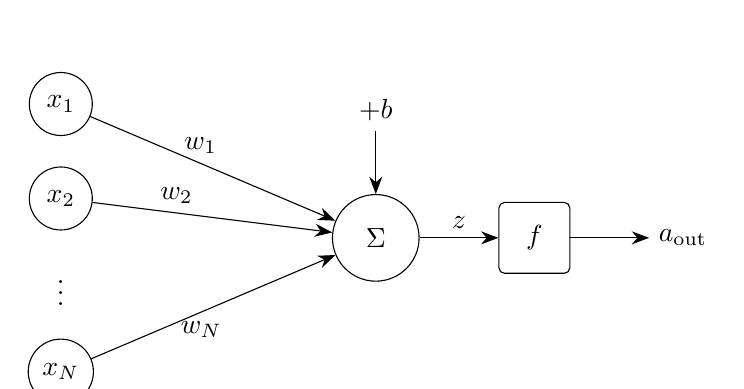
\begin{tikzpicture}[
  inp/.style={circle, draw, minimum size=8mm},
  >={Stealth[length=2.2mm]}
]
\node[inp] (x1) at (0,1.8) {$x_1$};
\node[inp] (x2) at (0,0.6) {$x_2$};
\node (xd) at (0,-0.5) {$\vdots$};
\node[inp] (xn) at (0,-1.6) {$x_N$};
\node[circle, draw, minimum size=11mm] (sum) at (4,0.1) {$\Sigma$};
\node[draw, rounded corners=2pt, minimum size=9mm, right=10mm of sum] (act) {$f$};
\node[right=10mm of act] (out) {$a_{\text{\lr{out}}}$};
\node[above=8mm of sum] (b) {$+b$};
\draw[->] (x1)--node[above,pos=.45]{$w_1$}(sum);
\draw[->] (x2)--node[above,pos=.35]{$w_2$}(sum);
\draw[->] (xn)--node[below,pos=.45]{$w_N$}(sum);
\draw[->] (b)--(sum);
\draw[->] (sum)--node[above]{$z$}(act);
\draw[->] (act)--(out);
\end{tikzpicture}
\caption{ساختار یک نورون: $z=b+\sum_i w_ix_i$ و سپس $a_{\text{\lr{out}}}=f(z)$.}
\end{figure}

\textbf{نقش بایاس.} \term{بایاس}{Bias} به مدل اجازه می‌دهد خروجی را مستقل از حاصل‌ضرب وزن‌ها و ورودی جابه‌جا کند. استاد مثال «کرایهٔ تاکسی» زد: حتی برای سفر لغوشده (مسافت صفر) یک هزینهٔ پایه وجود دارد. هندسی: رابطه از اجبار عبور از مبدأ آزاد می‌شود.

\textbf{تابع فعال‌سازی.} بدون آن، ترکیب هر تعداد لایه همچنان یک تبدیل خطی است، در حالی که مرز مفاهیم در دنیای واقعی غیرخطی است. \term{تابع فعال‌سازی}{Activation Function} (مانند \eng{Sigmoid}، \eng{tanh}، \eng{ReLU}) رفتار شبکه را از خط صاف به منحنی تبدیل می‌کند. برای \eng{Sigmoid}:
\[
\sigma(z)=\frac{1}{1+e^{-z}},\qquad \sigma'(z)=\sigma(z)\bigl(1-\sigma(z)\bigr).
\]

\begin{figure}[htbp]
\centering
\fbox{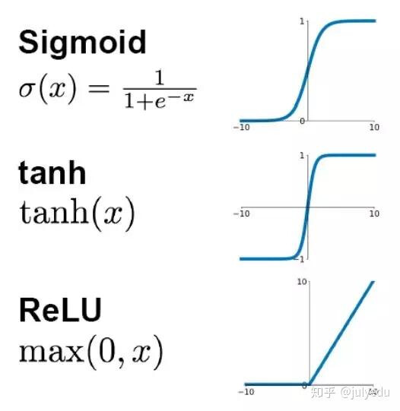
\includegraphics[width=0.28\textwidth]{../assets/figures/ch08-activations.png}}
\caption{\eng{Sigmoid}، \eng{tanh} و \eng{ReLU}. \textit{(برگرفته از تختهٔ کلاس)}}
\end{figure}

\subsection{تابع خطا، چشم‌انداز خطا و کاهش گرادیان}
خروجی با \eng{Ground Truth} مقایسه می‌شود؛ یک تابع خطا \term{میانگین مربعات خطا}{Mean Squared Error} است:
\[
\operatorname{MSE}=\frac{1}{n}\sum_{i=1}^{n}(y_i-\hat{y}_i)^2 ,
\]
که $y_i$ مقدار واقعی و $\hat y_i$ پیش‌بینی است. هدف آموزش کاهش این مقدار است.

استاد از مفهوم \term{چشم‌انداز خطا}{Loss Landscape} استفاده کرد: سطحی که ارتفاعش مقدار خطا و بقیهٔ ابعادش وزن‌هاست.

اگر مشتق خطا نسبت به وزن مثبت باشد، افزایش وزن خطا را زیاد می‌کند؛ پس باید در جهت \emph{مخالف} شیب حرکت کنیم («اگر از لاس مشتق بگیریم و مثبت شد، آن را در منفی ضرب می‌کنیم»). این مبنای \term{کاهش گرادیان}{Gradient Descent} است:
\[
\boxed{\,w_{\text{\lr{new}}}=w_{\text{\lr{old}}}-\eta\,\frac{\partial E}{\partial w}\,}
\]
که $\eta$ \term{نرخ یادگیری}{Learning Rate} (اندازهٔ گام) است: اگر بسیار کوچک باشد حرکت کند است، اگر مناسب باشد همگرا می‌شود و اگر بسیار بزرگ باشد از کمینه می‌پرد و ممکن است همگرا نشود.

\boardfigure{0.6}{ch08-learning-rate.png}{اثر نرخ یادگیری: بسیار کوچک، مناسب و بسیار بزرگ.}

\subsection{پس‌انتشار و قانون زنجیره‌ای}
سهم هر وزن در خطا با \term{قانون زنجیره‌ای}{Chain Rule} محاسبه می‌شود؛ این کار را
\term{پس‌انتشار}{Backpropagation} می‌نامند. برای نورون خروجی با
\[
\text{net}=h\,w_5+\cdots,\quad o=\sigma(\text{net}),\quad E=\tfrac12(y-o)^2 ,
\]
داریم:
\[
\frac{\partial E}{\partial w_5}=\frac{\partial E}{\partial o}\cdot\frac{\partial o}{\partial\,\text{net}}\cdot\frac{\partial\,\text{net}}{\partial w_5}
\]
\[
\boxed{\;\frac{\partial E}{\partial w_5}=(o-y)\,o\,(1-o)\,h\;}
\]
زیرا $\partial E/\partial o=o-y$ ، $\partial o/\partial\text{net}=o(1-o)$ و $\partial\text{net}/\partial w_5=h$.

\begin{figure}[htbp]
\centering
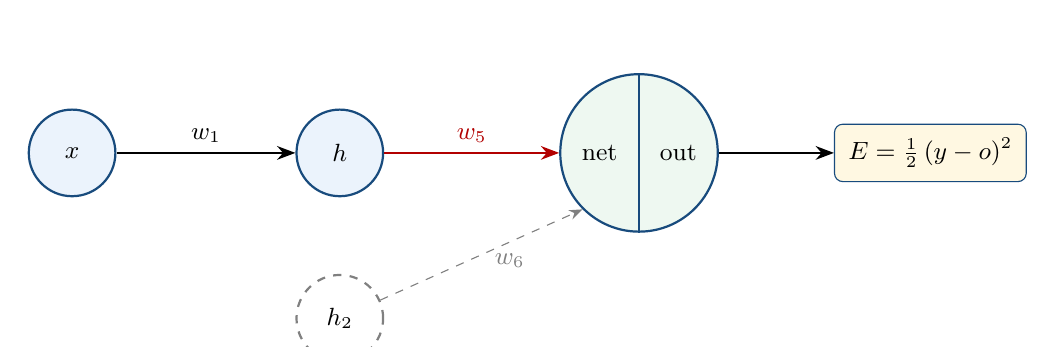
\begin{tikzpicture}[>=Stealth, font=\small]
\tikzset{unit/.style={circle,draw=mainblue,fill=softblue,minimum size=1.1cm,thick}}
\node[unit] (x) at (0,0) {$x$};
\node[unit] (h) at (3.4,0) {$h$};
\node[unit,minimum size=1.1cm,draw=gray,fill=white,dashed] (h2) at (3.4,-2.1) {$h_2$};
\node[circle,draw=mainblue,fill=softgreen,minimum size=2cm,thick] (o) at (7.2,0) {};
\draw[mainblue,thick] (o.north)--(o.south);
\node at ([xshift=-0.5cm]o.center) {\lr{net}};
\node at ([xshift=0.5cm]o.center) {\lr{out}};
\node[draw=mainblue,fill=softyellow,rounded corners=3pt,inner sep=5pt] (e) at (10.9,0) {$E=\tfrac12\,(y-o)^2$};
\draw[->,thick] (x) -- node[above] {$w_1$} (h);
\draw[->,thick,red!70!black] (h) -- node[above] {$w_5$} (o.west);
\draw[->,dashed,gray] (h2) -- node[below right,pos=0.55,inner sep=1pt] {$w_6$} (o.south west);
\draw[->,thick] (o.east) -- (e.west);
\end{tikzpicture}
\caption{شبکهٔ ساده برای پس‌انتشار و محاسبهٔ $\partial E/\partial w_5$.}
\end{figure}

\begin{correctionbox}{دقت در علامت و ضریب مشتق}
در کلاس علامت و ضریب مشتق به‌دقت تثبیت نشد. نتیجهٔ بالا برای $E=\frac12(y-o)^2$ است؛ برای تابع خطای دیگر (مثل \eng{Cross-Entropy}) جزء $\partial E/\partial o$ تغییر می‌کند و باید طبق تعریف دقیق همان تابع محاسبه شود.
\end{correctionbox}

\begin{addedbox}{مثال عددی: یک نورون، یک گام یادگیری}
ورودی $\mathbf{x}=(2,1)$، وزن‌ها $\mathbf{w}=(0.4,-0.3)$، $b=0.1$، \eng{Sigmoid} و هدف $y=1$. پیش‌رو: $z=0.6$، $o=\sigma(0.6)\approx0.646$، $E\approx0.0628$. پس‌انتشار: $\delta=(o-y)\,o\,(1-o)\approx-0.0811$ و گرادیان‌ها $\delta x_1\approx-0.162$ ، $\delta x_2\approx-0.081$ ، $\delta\approx-0.081$. با $\eta=1$: $w_1\approx0.562$ ، $w_2\approx-0.219$ ، $b\approx0.181$؛ اکنون $o\approx0.748$ و $E\approx0.0318$، یعنی خطا تقریباً نصف شد.
\end{addedbox}

چرخهٔ آموزش پنج گام دارد: مقداردهی تصادفی، \eng{Feedforward}، تولید خروجی، محاسبهٔ \eng{Loss} و \eng{Backpropagation} همراه با به‌روزرسانی وزن‌ها.

\section{مسئلهٔ هم‌نویسه در \eng{TTS}}

\term{هم‌نویسه}{Homograph} کلمه‌ای است با نوشتار یکسان و تلفظ (و معمولاً معنای) متفاوت. در فارسی چون بیشتر مصوت‌های کوتاه نوشته نمی‌شوند، این مسئله اهمیت ویژه‌ای دارد.

\begin{table}[htbp]
\centering
\caption{نمونه‌های هم‌نویسه در فارسی}
\begin{tabular}{c l l}
\toprule
کلمه & بافت اول & بافت دوم \\
\midrule
کرم & کرم مرطوب‌کننده (\eng{kerem}) & کرم خاکی (\eng{kerm}) \\
مرد & آن مرد وارد شد (\eng{mard}) & او از دنیا مرد (\eng{mord}) \\
سرم & سرم به شدت درد می‌کند (\eng{saram}) & سرم را از دستش کشیدند (\eng{serom}) \\
\bottomrule
\end{tabular}
\end{table}

\begin{correctionbox}{«شیر» هم‌نویسهٔ تلفظی نیست}
«شیر آب»، «شیر جنگل» و «شیر خوراکی» همگی \eng{/ʃir/} تلفظ می‌شوند؛ «شیر» کلمه‌ای \emph{چندمعنایی} (\eng{Homonym}) است نه هم‌نویسه با تلفظ‌های متفاوت. برای \eng{TTS} فقط مواردی مسئله‌ساز است که تلفظ‌ها فرق کنند (مانند «کرم» و «مرد»)؛ اما «شیر» مثال خوبی برای محدودیت \eng{Embedding} ثابت در فهم \emph{معناست}.
\end{correctionbox}

\textbf{نقش \eng{POS Tagging}.} گاهی \term{برچسب‌گذاری اجزای کلام}{POS Tagging} کافی است: «او مُرد» فعل و «آن مَرد» اسم است. اما «کِرم خاکی» و «کِرِم مرطوب‌کننده» هر دو اسم‌اند؛ پس به اطلاعات معنایی و بافتی، یعنی \eng{Contextual Embedding}، نیاز داریم. مثلاً «کرم خاکی» با باغچه و خاک هم‌وقوعی دارد و «کرم مرطوب‌کننده» با پوست و آرایش؛ بازنمایی کلمه باید این بافت را در خود داشته باشد.

\section{\eng{Embedding} ایستا و \eng{Word2Vec}}

\eng{Word2Vec} بر پایهٔ ارتباط هر کلمه با کلمات اطرافش آموزش می‌بیند و دو معماری دارد. بردارهای حاصل \term{ایستا}{Static} هستند: یک بردار ثابت برای هر مدخل واژگان.
\begin{itemize}
  \item \term{کیسهٔ کلمات پیوسته}{Continuous Bag of Words} (\eng{CBOW}): کلمات داخل یک \term{پنجرهٔ بافت}{Context Window} ورودی‌اند و مدل \emph{کلمهٔ مرکزی} را پیش‌بینی می‌کند (بافت $\leftarrow$ هدف)؛ بازنمایی کلمات اطراف جمع یا میانگین می‌شود.
  \item \eng{Skip-gram}: کلمهٔ مرکزی ورودی است و مدل \emph{کلمات اطراف} را پیش‌بینی می‌کند (هدف $\leftarrow$ بافت).
\end{itemize}

\begin{figure}[htbp]
\centering
\begin{tikzpicture}[rtl, >=Stealth, font=\small]
\tikzset{sq/.style={draw=mainblue,fill=softblue,minimum size=0.55cm,inner sep=0pt,thick},
 lab/.style={font=\scriptsize},
 note/.style={draw=mainblue,fill=softyellow,rounded corners=4pt,inner sep=5pt,text width=11.6cm,align=center}}
\node[note] at (5.8,4.7) {\lr{\textbf{Word2Vec}} — \lr{Static Embedding}: یک بردار ثابت برای هر کلمه\\
در زمان آموزش: \lr{Context-Based model}\\ در زمان استنتاج: \lr{Context-independent}};
% headers
\node[lab] at (0,3.1) {\lr{Input}}; \node[lab] at (2.2,3.1) {\lr{Projection}}; \node[lab] at (4.2,3.1) {\lr{Output}};
\node[lab] at (7.4,3.1) {\lr{Input}}; \node[lab] at (9.0,3.1) {\lr{Projection}}; \node[lab] at (11.0,3.1) {\lr{Output}};
% CBOW
\foreach \y/\t [count=\k] in {1.8/{W(t-2)},0.9/{W(t-1)},-0.9/{W(t+1)},-1.8/{W(t+2)}} {
  \node[sq] (c\k) at (0,\y) {}; \node[lab,left=1pt of c\k] {\lr{$\t$}}; }
\node[sq] (cp) at (2.2,0) {}; \node[lab] at (2.2,0.7) {\lr{Sum}};
\node[sq] (co) at (4.2,0) {}; \node[lab,right=1pt of co] {\lr{$W(t)$}};
\foreach \k in {1,2,3,4} \draw[->] (c\k.east) -- (cp.west);
\draw[->] (cp) -- (co);
\node[lab] at (2.2,-2.5) {(a) \lr{CBOW}};
% Skip-gram
\node[sq] (si) at (7.4,0) {}; \node[lab,left=1pt of si] {\lr{$W(t)$}};
\node[sq] (sp) at (9.0,0) {};
\draw[->] (si) -- (sp);
\foreach \y/\t [count=\k] in {1.8/{W(t-2)},0.9/{W(t-1)},-0.9/{W(t+1)},-1.8/{W(t+2)}} {
  \node[sq] (s\k) at (11.0,\y) {}; \node[lab,right=1pt of s\k] {\lr{$\t$}};
  \draw[->] (sp.east) -- (s\k.west); }
\node[lab] at (9.2,-2.5) {(b) \lr{Skip-gram}};
% goals
\node[text width=5cm,align=center,font=\footnotesize] at (1.8,-3.7) {هدف: پیش‌بینی کلمهٔ هدف \lr{(Target)} با استفاده از کلمات پیرامون \lr{(Context)}.};
\node[text width=5cm,align=center,font=\footnotesize] at (9.8,-3.7) {هدف: پیش‌بینی کلمات پیرامون \lr{(Context)} با دریافت یک کلمهٔ ورودی \lr{(Target)}.};
\node[draw=red!70!black,rounded corners=4pt,inner sep=5pt,text width=8cm,align=center,text=red!70!black,font=\footnotesize] at (5.8,-5.3) {برای کاری که کلمات نادر \mbox{\lr{(Rare words)}} زیادی دارد کدام بهتر است؟};
\end{tikzpicture}
\caption{دو معماری \eng{Word2Vec}: \eng{CBOW} و \eng{Skip-gram}، همراه با یادداشت‌های استاد روی تخته.}
\end{figure}

\begin{exambox}{پرسش استاد: برای کلمات نادر کدام بهتر است؟}
پاسخ: \eng{Skip-gram}. در \eng{CBOW} کلمهٔ نادر فقط در جایگاه «هدف» است و اطلاعات چند کلمه در یک بردار ادغام می‌شود، پس فرصت‌های یادگیری آن کم است. در \eng{Skip-gram} هر رخداد کلمهٔ نادر چند جفت آموزشی (کلمه، همسایه) می‌سازد. استاد افزود اگر داده نویز نداشته باشد حتی یک رخداد هم ممکن است اطلاعات مفیدی بدهد، اما یادگیری از نمونهٔ بسیار اندک همچنان محدود است.
\end{exambox}

\begin{correctionbox}{دقت دربارهٔ \eng{CBOW} و \eng{Word2Vec}}
در \eng{CBOW} کلمات پنجره میانگین یا جمع می‌شوند و ترتیب نقشی ندارد؛ پس همهٔ کلمات اطراف سهم برابر دارند و کلمهٔ مهم (مثلاً «مریض» برای پیش‌بینی «دکتر») وزن بیشتری نمی‌گیرد. همین انگیزهٔ مهم \eng{Attention} است. همچنین بردار مورد استفاده معمولاً از ماتریس ورودی (جدول جست‌وجو) برداشته می‌شود و در عمل برای کاهش هزینهٔ خروجی از \eng{Negative Sampling} یا \eng{Hierarchical Softmax} استفاده می‌شود. پس از آموزش فقط بردارها را نگه می‌داریم.
\end{correctionbox}

\section{محدودیت \eng{Embedding} ایستا در تشخیص هم‌نویسه}

مهم‌ترین نکتهٔ جلسه: تفاوت میان \eng{Embedding}ای که \emph{در زمان آموزش} از بافت ساخته شده و \eng{Embedding}ای که \emph{در زمان استفاده} به بافت جملهٔ جدید وابسته است.

در \eng{Word2Vec} برای «کرم» یک بردار ثابت داریم:
\[
E(\text{کرم در «کرم خاکی در باغچه بود»})=E(\text{کرم در «کرم مرطوب‌کننده را روی پوست زدم»}).
\]
این بردار در آموزش از همهٔ بافت‌ها ساخته شده (نوعی «میانگین»)، اما در استفاده برای همهٔ رخدادها یکسان است؛ پس به‌تنهایی تلفظ درست را مشخص نمی‌کند.

\textbf{راه‌حل با \eng{Embedding} ثابت:} در کنار آن یک مدل انتخاب تلفظ می‌گذاریم: \eng{Embedding} ثابت کلمه و کلمات اطراف هم‌نویسه را به مدل می‌دهیم، بخش پیش‌بینی‌کننده را با داده‌های دارای برچسب تلفظ آموزش می‌دهیم و مدل بر پایهٔ بافت تلفظ را برمی‌گزیند. اگر $z_i$ امتیاز (\eng{logit}) تلفظ $i$ام و $C$ بافت باشد:
\[
P(P_i\mid C)=\frac{e^{z_i}}{\sum_j e^{z_j}},\qquad
\hat P=\arg\max_i P(P_i\mid C).
\]
برای تعداد متفاوت تلفظ‌ها، استاد یک \eng{Linear Layer} و سپس \eng{Softmax} پیشنهاد کرد، به شرط آنکه مجموعهٔ گزینه‌ها از پیش مشخص باشد؛ معماری دقیق این بخش در جلسهٔ بعد بررسی می‌شود.

\section{چرا همهٔ تلفظ‌ها را از ابتدا برچسب نمی‌زنیم؟}
\label{sec:selfsup}

دانشجویی پیشنهاد کرد برای هر تلفظ از ابتدا یک بازنمایی جداگانه («کرم۱»، «کرم۲») داشته باشیم. استاد: از نظر مفهومی ممکن است، اما \emph{چه کسی باید تمام رخدادها را برچسب بزند؟} این کار بسیار پرهزینه است.

\begin{exambox}{تأکید استاد}
\term{برچسب‌گذاری}{Annotation} یکی از گلوگاه‌های مهم توسعهٔ سامانه‌های هوش مصنوعی است.
\end{exambox}

راه‌حل: وظایفی که برچسبشان از خود متن می‌آید، مانند \term{مدل‌سازی زبان نقاب‌دار}{Masked Language Modeling} (\eng{MLM}: پنهان‌کردن کلمات و پیش‌بینی آن‌ها) و \term{پیش‌بینی جملهٔ بعدی}{Next Sentence Prediction} (\eng{NSP} در \eng{BERT} اولیه). \eng{NSP} بیشتر یک نمونهٔ تاریخی است و پژوهش‌های بعدی (مانند \eng{RoBERTa}) نشان دادند حذفش آسیبی نمی‌زند؛ \eng{MLM} وظیفهٔ اصلی است.

\begin{definitionbox}{یادگیری نظارتی در برابر خودنظارتی}
در \term{یادگیری نظارتی}{Supervised Learning} انسان داده را برچسب می‌زند. در \term{یادگیری خودنظارتی}{Self-Supervised Learning} برچسب از خود داده ساخته می‌شود (مثلاً کلمهٔ حذف‌شده). نتیجه: نیاز به برچسب دستی کم می‌شود، استفاده از متن‌های بسیار بزرگ ممکن می‌شود و مدل بازنمایی عمومی می‌آموزد که بعداً تنظیم دقیق می‌شود. به تأکید استاد، یکی از جهش‌های بزرگ مدل‌های زبانی همین بود.
\end{definitionbox}

\section{\eng{Embedding} وابسته به بافت (پویا)}

برای اینکه \eng{Embedding} با جملهٔ ورودی تغییر کند، از \term{\eng{Embedding} وابسته به بافت}{Contextual Embedding} (پویا) استفاده می‌کنیم. در بازنمایی ایستا $E(w)=\mathbf{v}_w$ فقط به هویت کلمه بستگی دارد؛ در بازنمایی وابسته به بافت $E(w,C)=\mathbf{v}_{w,C}$ که $C$ جملهٔ حاوی کلمه است، و ممکن است $E(\text{کرم},C_1)\neq E(\text{کرم},C_2)$.

\begin{table}[htbp]
\centering
\caption{مقایسهٔ دو نوع \eng{Embedding} به روایت تختهٔ کلاس}
\begin{tabular}{p{3cm} p{5.5cm} p{5.5cm}}
\toprule
 & ایستا & وابسته به بافت \\
\midrule
تعریف & بردار خروجی تابعی از همهٔ جمله‌هایی است که کلمه در زمان آموزش در آن‌ها دیده شده & بردار خروجی تابعی از کل کلمات جملهٔ فعلی است \\
زمان استفاده & کلمه به‌تنهایی وارد جدول جست‌وجو می‌شود & کلمه در بستر جمله وارد شبکه می‌شود و بردار نهایی از رابطه با همسایه‌ها ساخته می‌شود \\
چیزی که دانلود می‌کنید & فایلی با یک سطر (مثلاً ۳۰۰ عدد) برای هر کلمه؛ «شیر» در هر معنا همان بردار است & وزن‌های شبکه (\eng{Weights \& Biases})؛ بردار کلمه تا ورود جمله وجود ندارد \\
\bottomrule
\end{tabular}
\end{table}

\section{استفاده از \eng{Attention} برای ساخت \eng{Embedding} وابسته به بافت}
\label{sec:attention}

\term{سازوکار توجه}{Attention Mechanism} سه گام دارد: (۱) نمایش همهٔ موقعیت‌های ورودی را در اختیار داشته باش؛ (۲) ارتباط هر موقعیت را با بقیه محاسبه کن؛ (۳) بر اساس وزن‌های ارتباط، اطلاعات موقعیت‌ها را ترکیب کن تا نمایش جدید هر موقعیت به‌دست آید. به‌جای ترکیب یکسان همهٔ کلمات اطراف (مانند \eng{CBOW}) مدل می‌سنجد هر کلمه چقدر مرتبط است.

\begin{itemize}
  \item \term{پرس‌وجو}{Query} ($Q$): نمایندهٔ چیزی که برایش اطلاعات می‌جوییم (کلمهٔ هدف).
  \item \term{کلید}{Key} ($K$): برای سنجش ارتباط هر کلمه با پرس‌وجو.
  \item \term{مقدار}{Value} ($V$): اطلاعاتی که بر اساس میزان ارتباط در خروجی شرکت می‌کند.
\end{itemize}
شباهت \eng{Query} و \eng{Key} (ضرب داخلی) میزان توجه به هر کلمه را می‌دهد و \eng{Value}ها با این وزن‌ها ترکیب می‌شوند. ماتریس‌های وزنی $Q$، $K$ و $V$ در آموزش یاد گرفته می‌شوند و در استنتاج ثابت‌اند؛ آنچه با جمله عوض می‌شود بردارهای محاسبه‌شده و در نتیجه خروجی است. استاد تصریح کرد \eng{Attention} فقط یک ضرب ساده نیست و هدف این جلسه درک شهودی بود. فرمول کامل:
\[
\operatorname{Attention}(Q,K,V)=\operatorname{softmax}\!\left(\frac{QK^{\top}}{\sqrt{d_k}}\right)V ,
\]
که تقسیم بر $\sqrt{d_k}$ از اشباع \eng{Softmax} در بُعد زیاد جلوگیری می‌کند.

وقتی کلمات یک توالی به کلمات همان توالی توجه می‌کنند، به آن \term{خودتوجهی}{Self-Attention} می‌گویند: اگر «کرم» کنار «خاکی» و «باغچه» بیاید بازنمایی موجود زنده ساخته می‌شود و اگر کنار «پوست» و «مرطوب‌کننده» بیاید بازنمایی دیگری. \eng{Self-Attention} هستهٔ \term{ترنسفورمر}{Transformer} است که در ادامهٔ درس می‌آید. تفاوت اصلی با \eng{Word2Vec}: شبکه در استنتاج نیز با هر جملهٔ جدید اجرا می‌شود.

\begin{correctionbox}{دقت دربارهٔ «بردار ثابت» و «بردار پویا»}
در بازنمایی وابسته به بافت وزن‌های شبکه در استنتاج عوض نمی‌شوند؛ فقط \emph{خروجی} به‌ازای جملهٔ ورودی متفاوت است. همچنین \eng{Contextual Embedding} با \eng{Transformer} یکی نیست: \eng{LSTM} دوسویه (مانند \eng{ELMo}) نیز چنین بازنمایی می‌سازد و \eng{Attention} یکی از راه‌هاست.
\end{correctionbox}

\section{پرسش و پاسخ پایان کلاس و ادامهٔ بحث}
\label{sec:qa}

استاد از دانشجویان پرسید آیا مباحث شبکهٔ عصبی باید با جزئیات بیشتر (مانند \term{مومنتوم}{Momentum}) تدریس شوند و قرار شد همین سطح مقدماتی حفظ شود. جلسهٔ بعد: بررسی دقیق‌تر لایهٔ خروجی انتخاب تلفظ و \eng{Softmax}، ادامهٔ معماری‌های مبتنی بر بافت و ورود به \eng{Transformer}.

\section{جمع‌بندی}

کلمه ابتدا با \eng{One-Hot} نمایش داده می‌شود که پراکنده است و شباهت معنایی ندارد. \eng{Embedding} متراکم و آموخته‌شده این کمبود را جبران می‌کند و \eng{Word2Vec} آن را از هم‌وقوعی کلمات می‌سازد. اما بردار \eng{Word2Vec} ایستاست و برای «کرم» در همهٔ جمله‌ها یکسان می‌ماند؛ پس برای \eng{TTS} یا مدلی روی بافت می‌گذاریم و با داده‌های برچسب‌دار آموزش می‌دهیم، یا از بازنمایی وابسته به بافت بهره می‌گیریم. چون برچسب‌گذاری دستی گران است، پیش‌آموزش خودنظارتی (مانند \eng{MLM}) اهمیت می‌یابد و \eng{Self-Attention} ابزار اصلی ساخت این بازنمایی‌هاست.

\begin{exambox}{نکات مهم برای مرور و امتحان}
\begin{itemize}
  \item تفاوت \eng{Pipeline} و \eng{End-to-End}؛ تعریف \eng{Front-End} و \eng{Back-End}.
  \item چهار محدودیت \eng{One-Hot} و مزایای \eng{Embedding} (تراکم، بُعد کم، شباهت معنایی، آموخته از داده).
  \item چرخهٔ آموزش: مقداردهی تصادفی، \eng{Feedforward}، \eng{Loss}، \eng{Backpropagation} و به‌روزرسانی؛ رابطهٔ $w_{\text{\lr{new}}}=w_{\text{\lr{old}}}-\eta\,\partial E/\partial w$ و اثر نرخ یادگیری.
  \item نقش بایاس (مثال کرایهٔ تاکسی) و تابع فعال‌سازی (غیرخطی‌کردن).
  \item \eng{CBOW} در برابر \eng{Skip-gram}؛ برای کلمات نادر \eng{Skip-gram} بهتر است.
  \item \eng{Embedding} ایستا: در آموزش وابسته به بافت، در استنتاج مستقل از بافت؛ چرا برای هم‌نویسه کافی نیست.
  \item چرا همهٔ تلفظ‌ها را برچسب نمی‌زنیم (گلوگاه \eng{Annotation}) و نقش \eng{Self-Supervised Learning}.
  \item مفاهیم \eng{Query}/\eng{Key}/\eng{Value} و فرمول \eng{Attention}.
\end{itemize}
\end{exambox}

\chapter{آموزش شبکه، Embedding بافتی و تبدیل نویسه به واج}

این فصل سه بخش دارد: مرور آموزش شبکه (لایهٔ خروجی، آموزش در برابر استنتاج، بیش‌برازش)؛ \eng{Embedding}های بافتی، \eng{BERT}، قیاس برداری و \term{کاوش}{Probing}؛ و بازگشت به \eng{TTS} برای یافتن تلفظ درست هر واژه (هم‌نویسه‌ها و \eng{G2P}). مفاهیم پایهٔ آموزش (انتشار رو‌به‌جلو، خطا، پس‌انتشار، $w_{\text{new}}=w_{\text{old}}-\eta\,\partial E/\partial w$) در فصل قبل آمده‌اند.

\section{مرور فرایند آموزش شبکهٔ عصبی}

\subsection{طراحی لایهٔ خروجی بر اساس نوع مسئله}
نکتهٔ مورد تأکید استاد: \emph{خروجی شبکه باید با \eng{Task} هم‌خوان طراحی شود.}

\begin{table}[htbp]
\centering
\small
\begin{tabular}{p{2.6cm}p{3.4cm}p{3.3cm}p{3.5cm}}
\toprule
\textbf{نوع مسئله} & \textbf{لایهٔ خروجی} & \textbf{تابع خطا} & \textbf{مثال}\\
\midrule
\eng{Regression} & یک خروجی خطی (مقدار پیوسته) & \eng{MSE} & پیش‌بینی فرکانس پایه\\
\eng{Binary Classification} & یک خروجی \eng{Sigmoid} و آستانه‌گذاری & \eng{Binary Cross-Entropy} & واکدار/بی‌واک، گفتار/سکوت\\
\eng{Multi-class Classification} & \eng{Softmax} روی \eng{K} کلاس & \eng{Cross-Entropy} & نوع احساس صدا، تلفظ درست یک واژه\\
\bottomrule
\end{tabular}
\caption{ارتباط نوع مسئله با لایهٔ خروجی و تابع خطا.}
\end{table}

\begin{itemize}
  \item \textbf{رگرسیون:} اگر شبکه بردار $X\in\mathbb{R}^{1\times 768}$ ساخته باشد، یک لایهٔ خطی $W\in\mathbb{R}^{768\times1}$ می‌دهد $Y=XW+b$. اگر مسئله پیچیده‌تر باشد، \eng{Linear $\rightarrow$ Activation $\rightarrow$ Linear} (یک \eng{MLP}) به‌کار می‌رود؛ استاد تأکید کرد پیچیده‌ترکردن باید بر اساس عملکرد باشد.
  \item \textbf{دودویی:} خروجی یک \term{لاجیت}{Logit} است که از سیگموید $\sigma(x)=1/(1+e^{-x})\in(0,1)$ می‌گذرد؛ مثلاً $0.8$ یعنی احتمال کلاس مثبت ۸۰ درصد، و با یک آستانه (\eng{Threshold}) کلاس نهایی تعیین می‌شود.
  \item \textbf{چندکلاسه:} \eng{Softmax} لاجیت‌ها را به توزیع احتمال با مجموع ۱ تبدیل می‌کند:
\end{itemize}
\[
P(y=i)=\frac{e^{z_i}}{\sum_{j=1}^{K}e^{z_j}},\qquad \sum_{i=1}^{K}P(y=i)=1 .
\]
در پیش‌بینی توکن بعدی با واژگان $V$ توکن، بردار $1\times768$ در ماتریس $768\times V$ ضرب می‌شود و بردار لاجیت $1\times V$ حاصل می‌شود.

\subsection{تابع خطا و مثال پیش‌بینی توکن بعدی}
برای برچسب \eng{One-Hot}، \eng{Cross-Entropy} ساده می‌شود به
$L=-\sum_k y_k\log \hat y_k = -\log \hat y_{c}$
که در آن $c$ کلاس درست است؛ یعنی فقط احتمالی که مدل به پاسخ درست داده اهمیت دارد. مثال استاد: اگر احتمال پاسخ درست $0.2$ باشد، خطا $-\log 0.2\approx 1.61$ است؛ پس از چند گام اصلاح وزن‌ها و رسیدن احتمال به $0.9$، خطا به $-\log 0.9\approx 0.105$ کاهش می‌یابد. یعنی شبکه یاد می‌گیرد به پاسخ درست احتمال بیشتری بدهد.

\section{آموزش در برابر استنتاج}

در فاز \term{آموزش}{Training} پاسخ درست را داریم و خطا را حساب می‌کنیم؛ در فاز \term{استنتاج}{Inference} پاسخ درست در دسترس نیست و شبکه فقط یک توزیع احتمال می‌دهد. پرسش این است که از آن توزیع چگونه خروجی نهایی را برداریم.

\begin{table}[htbp]
\centering
\small
\begin{tabular}{p{3.0cm}p{5.4cm}p{5.6cm}}
\toprule
 & \textbf{آموزش} & \textbf{استنتاج}\\
\midrule
حقیقت مبنا & در دسترس است & در دسترس نیست\\
هدف & کمینه‌کردن خطا و اصلاح وزن‌ها & گرفتن خروجی از توزیع احتمال\\
وزن‌ها & در حال تغییرند & ثابت‌اند\\
\eng{Dropout} & فعال & غیرفعال\\
انتخاب خروجی & لازم نیست & \eng{Greedy}، \eng{Sampling}، \eng{Top-k}، \eng{Top-p}، \eng{Temperature}\\
\bottomrule
\end{tabular}
\caption{مقایسهٔ آموزش و استنتاج.}
\end{table}

\begin{itemize}
  \item \term{رمزگشایی حریصانه}{Greedy Decoding}: انتخاب پراحتمال‌ترین گزینه، $y=\arg\max_i P(y=i)$؛ روشی قطعی (برای $(0.6,0.3,0.1)$ همیشه گزینهٔ اول).
  \item \term{نمونه‌گیری}{Sampling}: خروجی از روی توزیع نمونه‌برداری می‌شود و گزینه‌های کم‌احتمال‌تر هم شانس دارند؛ مفید برای تنوع (مثلاً متن خلاقانه).
  \item \eng{Top-k}: فقط $k$ گزینهٔ پراحتمال نگه داشته می‌شود؛ \term{\eng{Top-p}}{Nucleus Sampling}: کوچک‌ترین مجموعه‌ای که مجموع احتمالش دست‌کم $p$ (مثلاً $0.9$) باشد؛ نمونه‌گیری فقط از همان مجموعه.
\end{itemize}

\subsection{دما (\eng{Temperature})}
دما تیزی توزیع را تنظیم می‌کند؛ لاجیت‌ها پیش از \eng{Softmax} بر $T$ تقسیم می‌شوند: $P_i=e^{z_i/T}/\sum_j e^{z_j/T}$. با $T=1$ \eng{Softmax} معمولی است؛ با $T\to0$ توزیع تیز و نزدیک به \eng{argmax} می‌شود؛ با $T$ بزرگ توزیع هموار و در حد، یکنواخت می‌گردد. دمای بالا تنوع را بیشتر می‌کند ولی احتمال خروجی نامناسب (\eng{Hallucination}) هم بالاتر می‌رود؛ دمای پایین خروجی را تکرارپذیرتر می‌کند. (مثلاً برای لاجیت $(2.0,1.0,0.1)$: $T=1$ احتمال‌های $(0.66,0.24,0.10)$ و $T=0.2$ تقریباً $(0.99,0.01,0.00)$ می‌دهد.) دما لاجیت‌های یادگرفته‌شده را عوض نمی‌کند و فقط شیوهٔ تبدیل آن‌ها به احتمال را در تولید تغییر می‌دهد.


\section{تعمیم‌پذیری: کم‌برازش، بیش‌برازش و پیچیدگی مدل}

برای فهمیدن اینکه مدل به‌اندازهٔ کافی آموزش دیده، خطای آموزشی کافی نیست؛ مدل باید روی داده‌ای ارزیابی شود که در به‌روزرسانی وزن‌ها به‌کار نرفته است. پس داده را به \eng{Training} (یادگیری وزن‌ها)، \eng{Validation} (پایش، توقف، انتخاب ابرپارامتر) و \eng{Test} (گزارش نهایی) تقسیم می‌کنیم؛ مجموعهٔ آزمون نباید برای تنظیم مدل به‌کار رود.

\subsection{سه وضعیت پس از آموزش}
\begin{itemize}
  \item \term{کم‌برازش}{Underfitting}: مدل حتی داده‌های آموزشی را هم خوب یاد نگرفته است.
  \item \term{برازش مناسب}{Good Fit}: الگوهای اصلی آموخته شده و روی داده‌های تازه هم خوب عمل می‌کند.
  \item \term{بیش‌برازش}{Overfitting}: مدل علاوه بر الگوی اصلی، نویز و جزئیات نامربوط داده آموزشی را حفظ کرده و تعمیم نمی‌دهد.
\end{itemize}

\begin{exambox}{مثال استاد از بیش‌برازش در گفتار}
در داده‌های آموزشی یک دستیار صوتی، هر بار که عبارت خاصی گفته شده صدای فن هم در پس‌زمینه بوده است. مدل ممکن است صدای فن را نشانهٔ آن عبارت بگیرد؛ روی داده آموزشی خوب عمل می‌کند ولی روی همان عبارت بدون صدای فن اشتباه می‌کند.
\end{exambox}

\subsection{منحنی خطا و توقف زودهنگام}
با افزایش \eng{Epoch}، خطای آموزش معمولاً کم می‌شود؛ خطای اعتبارسنجی نخست کم می‌شود ولی از جایی ممکن است دوباره بالا برود. کمینهٔ آن بهترین نقطه است و افزایش خطای اعتبارسنجی همراه با کاهش خطای آموزش نشانهٔ بیش‌برازش است. توقف آموزش در این نقطه \term{توقف زودهنگام}{Early Stopping} نام دارد.

\coursefigure{0.85}{ch09-loss-curves.png}{سه رفتار نوعی در طول آموزش (سه نمودار اول) و رابطهٔ خطا با پیچیدگی مدل (نمودار آخر). مقادیر شبیه‌سازی‌شده‌اند و فقط برای نمایش مفهوم‌اند. (شکل افزوده)}

\subsection{\eng{Bias} و \eng{Variance}}
\begin{table}[htbp]
\centering
\small
\begin{tabular}{p{2.8cm}p{5.6cm}p{5.8cm}}
\toprule
 & \textbf{\eng{High Bias} (کم‌برازش)} & \textbf{\eng{High Variance} (بیش‌برازش)}\\
\midrule
نشانه & خطای آموزش و اعتبارسنجی هر دو زیاد و نزدیک به هم & خطای آموزش کم، خطای اعتبارسنجی بسیار بیشتر\\
راهکار & مدل را پیچیده‌تر کن: لایه و نورون بیشتر، یا معماری مناسب‌تر & داده با کیفیت‌تر، بررسی ناسازگاری برچسب‌ها، متعادل‌کردن داده، \eng{Data Augmentation}، \eng{Regularization}\\
\bottomrule
\end{tabular}
\caption{مقایسهٔ بایاس بالا و واریانس بالا.}
\end{table}

\begin{exambox}{تا کجا مدل را پیچیده‌تر کنیم؟}
تا جایی که خطای اعتبارسنجی بهتر می‌شود؛ معماری را بر پایهٔ عملکرد تغییر دهید، نه صرفاً با افزودن لایه و نورون.
\end{exambox}

\subsection{\eng{Regularization}}
\term{منظم‌سازی}{Regularization} هر روشی است که پیچیدگی مؤثر مدل را محدود می‌کند تا تعمیم بهتر شود.
\begin{itemize}
  \item \eng{Dropout}: در هر گام آموزش، خروجی تعدادی از نورون‌ها تصادفی صفر می‌شود تا شبکه به مسیر یا ویژگی خاصی بیش‌ازحد تکیه نکند.
  \item \eng{L1} و \eng{L2}: جملهٔ جریمهٔ وزن‌های بزرگ به خطا افزوده می‌شود، $L_{\text{total}}=L_{\text{task}}+\lambda\sum_i |w_i|$ (\eng{L1}) یا $L_{\text{task}}+\lambda\sum_i w_i^2$ (\eng{L2}) که $\lambda$ شدت منظم‌سازی است.
\end{itemize}

\begin{exambox}{پرسش: اگر وزن بزرگ برای یک ویژگی واقعاً خوب باشد چه؟}
پاسخ استاد: منظم‌سازی بین وزن مفید و نامفید تمایز مستقیم نمی‌گذارد؛ اگر وزن بزرگی واقعاً لازم باشد، میان کاهش خطا و جریمهٔ وزن مصالحه شکل می‌گیرد و شبکه عمیق با ترکیب ویژگی‌های زیاد عملکرد را حفظ می‌کند. $\lambda$ را با خطای اعتبارسنجی انتخاب کنید و ویژگی‌ها را هم‌مقیاس (\eng{Scaling}) کنید، چون جریمهٔ وزن به مقیاس ورودی حساس است.
\end{exambox}

\section{\eng{Embedding} ایستا و پویا (بافتی)}

\eng{Embedding} نمایش واژه‌ها یا توکن‌ها با بردارهای عددی چگال است (در برابر بردار تُنُک \eng{One-Hot}). لایهٔ \eng{Embedding} دو شاخه دارد: ایستا (\eng{Static}) و پویا یا بافتی (\eng{Contextual}).



\begin{itemize}
  \item \textbf{ایستا:} هر روشی که بردار هر واژه تابعی از جمله‌های زمان آموزش باشد. نمونهٔ مهم \eng{Word2Vec} (\eng{CBOW}، \eng{Skip-gram}) است: بردارها با یک \eng{Task} آموزشی تنظیم می‌شوند و پس از آموزش، بخش پیش‌بینی کنار گذاشته و فقط بردارها نگه داشته می‌شوند. در زمان استفاده، واژه تنها و بدون دیدن جمله وارد یک \term{جدول جست‌وجو}{Lookup Table} می‌شود؛ مثلاً «شیر» یک سطر ۳۰۰تایی دارد، چه منظور شیر جنگل باشد چه شیر آب. جمع‌بندی استاد: در آموزش \eng{Context-based}، در استنتاج \eng{Context-independent}.
  \item \textbf{پویا:} بردار واژه تابعی از کل جملهٔ فعلی است. جمله وارد شبکه می‌شود و بردار بر اساس رابطهٔ واژه با همسایه‌هایش ساخته می‌شود:
\end{itemize}
\[
\text{ایستا: } E(w)=v_w,\qquad \text{بافتی: } E(w,C)=v_{w,C},\qquad E(\text{شیر},C_1)\neq E(\text{شیر},C_2).
\]
آنچه دانلود می‌کنیم وزن‌ها و بایاس‌های شبکه است و بردار واژه تا ورود جمله وجود ندارد. پس بردار ایستا را می‌توان جدا ذخیره کرد، ولی برای بردار بافتی باید خود مدل اجرا شود.

\begin{table}[htbp]
\centering
\small
\begin{tabular}{p{3.0cm}p{5.5cm}p{5.5cm}}
\toprule
 & \textbf{ایستا (\eng{Static})} & \textbf{پویا (\eng{Contextual})}\\
\midrule
بردار هر واژه & ثابت، یکی برای هر واژه & وابسته به جمله؛ هر رخداد بردار خودش را دارد\\
زمان استفاده & جست‌وجو در جدول (بدون شبکه) & اجرای شبکه روی کل جمله\\
خروجی دانلودی & فایل جدول بردارها & وزن‌های شبکه\\
نمونه & \eng{Word2Vec}، \eng{GloVe} & \eng{ELMo}، \eng{BERT}\\
\bottomrule
\end{tabular}
\caption{مقایسهٔ \eng{Embedding} ایستا و بافتی.}
\end{table}

\begin{correctionbox}{«شیر» هم‌نویسهٔ \eng{TTS} نیست}
«شیر» در هر سه معنا (جنگل، خوراکی، شیرآب) یک‌جور تلفظ می‌شود (\lr{/ʃiːr/})؛ پس مثال خوبی برای \emph{چندمعنایی} و محدودیت \eng{Embedding} ایستاست، اما \eng{Homograph} به‌معنای «هم‌نویسه با تلفظ متفاوت» نیست. برای \eng{TTS} از «مَرد/مُرد» و «کِرم/کَرَم» استفاده می‌کنیم.
\end{correctionbox}

\eng{Embedding} بافتی فقط برای رفع ابهام معنایی نیست؛ مثلاً در \term{تشخیص مرجع ضمیر}{Coreference Resolution} («من این کتاب را به علی دادم. او …») بردار باید «او» را به «علی» ربط دهد. اینکه هر لایه چه اطلاعاتی دارد را با \eng{Probing} می‌سنجیم (بخش~\ref{sec:ch09-probing}).

\section{راه‌های ساخت \eng{Embedding} بافتی}

مسئلهٔ اصلی: \emph{چگونه بردار یک واژه را وابسته به متن پیرامونش بسازیم؟} استاد تأکید کرد که \eng{Contextual Embedding} را نباید با \eng{Transformer} یکی دانست؛ ابتدا باید مسئله را فهمید و بعد سراغ معماری رفت. دو رویکرد مطرح شد:

\begin{itemize}
  \item \textbf{نگاه موازی (\eng{Self-Attention}):} نمایش همهٔ موقعیت‌ها را در اختیار داشته باش؛ ارتباط هر موقعیت با بقیه را حساب کن؛ بر اساس وزن‌های ارتباط اطلاعات را ترکیب کن تا نمایش جدید هر موقعیت ساخته شود. به زبان \eng{Query}/\eng{Key}/\eng{Value}: واژهٔ موردنظر (\eng{Query}) با \eng{Key} بقیه مقایسه می‌شود و ترکیب وزن‌دار \eng{Value}ها بردار جدید را می‌دهد.
  \item \textbf{نگاه ترتیبی (\eng{RNN}/\eng{LSTM}):} ورودی‌ها به‌ترتیب پردازش می‌شوند و \term{حالت پنهان}{Hidden State} خلاصه‌ای از توکن‌های قبلی را به گام بعد می‌برد. \eng{LSTM} با دروازه‌ها (\eng{Gating}) وابستگی‌های بلندتر را بهتر نگه می‌دارد و \eng{BiLSTM} هر دو بافت چپ و راست را به‌کار می‌گیرد.
\end{itemize}

\begin{correctionbox}{\eng{Attention} هم‌ارز \eng{Transformer} نیست}
\eng{Attention} حدود ۲۰۱۴ برای ترجمهٔ ماشینی با شبکه‌های بازگشتی معرفی شد و \eng{Transformer} (۲۰۱۷) معماری‌ای است که تماماً بر \eng{Self-Attention} تکیه دارد. سه مفهوم را جدا بدانید: مسئلهٔ ساخت بازنمایی بافتی، سازوکار \eng{Attention}، و معماری \eng{Transformer}.
\end{correctionbox}

\section{یادگیری خودنظارتی و \eng{BERT}}

یادگیری بازنمایی بافتی به داده بسیار زیاد نیاز دارد و برچسب‌گذاری انسانی گران است. راه‌حل \term{یادگیری خودنظارتی}{Self-Supervised Learning} است: برچسب از خود داده ساخته می‌شود (در \eng{Supervised} انسان برچسب می‌زند؛ در \eng{Self-supervised} مثلاً واژهٔ حذف‌شده از متن اصلی برچسب است). \eng{BERT} با دو \eng{Task} پیش‌آموزش می‌شود:

\begin{itemize}
  \item \term{مدل‌سازی زبان ماسک‌شده}{Masked Language Modeling, MLM}: بخشی از متن پوشانده می‌شود («امروز هوا \lr{[MASK]} است.») و مدل باید آن را پیش‌بینی کند. چون واژهٔ اصلی را داریم، حقیقت مبنا داریم: خروجی را با واژهٔ واقعی مقایسه، \eng{Cross-Entropy} حساب، پس‌انتشار و به‌روزرسانی می‌کنیم.
  \item \term{پیش‌بینی جملهٔ بعدی}{Next Sentence Prediction, NSP}: دو جمله داده می‌شود و مدل می‌گوید آیا جملهٔ دوم ادامهٔ واقعی اول است (نمونهٔ مثبت) یا جملهٔ تصادفی (نمونهٔ منفی)؛ یک دسته‌بندی دودویی. بردار ۷۶۸‌بعدی توکن \lr{[CLS]} در یک لایهٔ $768\times2$ ضرب می‌شود تا دو لاجیت (\eng{IsNext}/\eng{NotNext}) به دست آید.
\end{itemize}

\begin{figure}[htbp]
  \centering
  \fbox{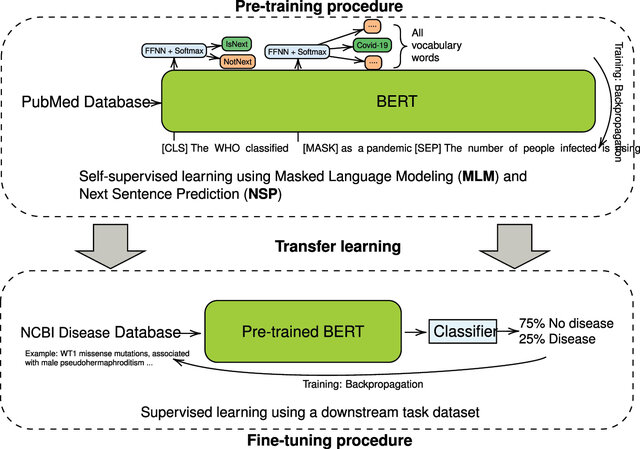
\includegraphics[width=0.6\textwidth]{../assets/figures/ch09-board-emb-img04.png}}
  \caption{فرایند پیش‌آموزش و انتقال یادگیری برای \eng{BERT}: بالا، پیش‌آموزش خودنظارتی با \eng{MLM} و \eng{NSP} (دو سر خروجی روی مدل)؛ پایین، قرار دادن یک دسته‌بند روی \eng{BERT} پیش‌آموزش‌دیده و آموزش تکمیلی با داده برچسب‌دار \eng{Task} هدف. \textit{(برگرفته از تختهٔ کلاس)}}
  \label{fig:ch09-bert}
\end{figure}

\eng{BERT} یک \eng{Transformer Encoder} دوطرفه است. \eng{BERT-Base}: ۱۲ لایه، بُعد ۷۶۸، حدود ۱۱۰ میلیون پارامتر؛ \eng{BERT-Large}: ۲۴ لایه، بُعد ۱۰۲۴. برای ورودی با ۷۱ توکن، خروجی هر لایه $H\in\mathbb{R}^{71\times768}$ است (یک بردار برای هر توکن). سر \eng{MLM} روی لایهٔ ۱۲ قرار می‌گیرد: بردار $1\times768$ موقعیت ماسک با لایهٔ $768\times768$ و سپس $768\times V$ به لاجیت‌هایی به‌طول $V=30522$ می‌رسد و \eng{Softmax} احتمال هر واژهٔ فرهنگ را می‌دهد.

\begin{correctionbox}{جزئیات دقیق \eng{BERT} و وضعیت \eng{NSP}}
در \eng{MLM} حدود ۱۵ درصد توکن‌ها انتخاب می‌شوند (۸۰ درصد با \lr{[MASK]}، ۱۰ درصد توکن تصادفی، ۱۰ درصد بدون تغییر). پژوهش‌هایی مانند \eng{RoBERTa} نشان دادند حذف \eng{NSP} آسیبی نمی‌زند؛ پس \eng{NSP} ضروری نیست. عدد $30522$ اندازهٔ واژگان \eng{bert-base-uncased} است و $V$ به مدل بستگی دارد.
\end{correctionbox}

پس از پیش‌آموزش، سر \eng{MLM} حذف و وزن‌های لایه‌ها نگه داشته می‌شود. دو شیوهٔ استفاده:
\begin{enumerate}
  \item \textbf{استخراج بردار}: جمله را به شبکه می‌دهیم؛ خروجی لایهٔ ۱۲ برای هر واژه یک بردار ۷۶۸‌تایی است (\eng{Embedding} بافتی آن واژه)، و میانگین روی واژه‌ها یک \eng{Embedding} برای کل جمله می‌دهد.
  \item \textbf{انتقال یادگیری} (\eng{Transfer Learning}): روی شبکه یک دسته‌بند می‌گذاریم و با داده‌ای محدود و مرتبط با \eng{Task} خود آموزش تکمیلی (\eng{Fine-tuning}) می‌دهیم.
\end{enumerate}

\begin{exambox}{آیا افزودن لایهٔ بیشتر (\eng{Linear} یا \eng{MLP}) همیشه بهتر است؟}
نمی‌توان قطعی گفت؛ اگر یک لایهٔ ساده کافی است، پیچیده‌ترکردن لازم نیست، و تصمیم بر اساس خطای آموزش و اعتبارسنجی و بایاس/واریانس گرفته می‌شود.
\end{exambox}

\section{قیاس برداری (\eng{Analogy}) در فضای \eng{Embedding}}

اگر روابط معنایی یا ساختاری در فضای \eng{Embedding} خوب بازتاب یافته باشند، اختلاف بردارهای دو جفت واژهٔ هم‌رابطه تقریباً یکسان است:
\[
\vec{v}_{\text{\lr{king}}}-\vec{v}_{\text{\lr{man}}}+\vec{v}_{\text{\lr{woman}}}\approx\vec{v}_{\text{\lr{queen}}}
\quad\Longleftrightarrow\quad
\vec{v}_{\text{\lr{woman}}}-\vec{v}_{\text{\lr{man}}}\approx\vec{v}_{\text{\lr{queen}}}-\vec{v}_{\text{\lr{king}}} .
\]
یعنی «جهت» مفهوم زن‌بودن در برابر مرد‌بودن در دو جفت یکی است. استاد توضیح داد چنین الگوهایی نشانهٔ سازمان‌یافتگی مفید فضا هستند اما برای همهٔ واژه‌ها و مدل‌ها تضمین‌شده نیستند.

همین ایده در گفتار هم مطرح است: مقالهٔ «\lr{[b] = [d] − [t] + [p]}» (چوی و همکاران) گزارش می‌کند که در بازنمایی مدل‌های گفتاری خودنظارتی، جهت‌های خطی متناظر با ویژگی‌های واجی وجود دارد؛ تفاضل $[d]-[t]$ یک «بردار واک‌داری» (\eng{Voicing}) است و افزودن آن به $[p]$ تقریباً $[b]$ می‌دهد. روی تخته:
\[
\vec{v}_{[d]}-\vec{v}_{[t]}+\vec{v}_{[p]}\approx\vec{v}_{[b]},\qquad\text{یعنی}\qquad \vec{v}_{[d]}-\vec{v}_{[t]}\approx\vec{v}_{[b]}-\vec{v}_{[p]}.
\]
کاربردهای مطرح‌شده در کلاس: کشف ویژگی‌های آموخته‌شدهٔ مدل، بررسی لهجه و کاربرد احتمالی در سنتز و \eng{Voice Cloning} (ایده‌ای قابل بررسی، نه نتیجهٔ قطعی).

\begin{correctionbox}{محدودیت‌های قیاس برداری}
قیاس‌هایی مانند king - man + woman در مثال‌های خوب‌انتخاب‌شده و \eng{Embedding} ایستا دیده می‌شوند اما همیشه برقرار نیستند و می‌توانند سوگیری داده را منعکس کنند؛ ابزاری شهودی است، نه قانون.
\end{correctionbox}

\section{کاوش (\eng{Probing}) و تفسیرپذیری}
\label{sec:ch09-probing}

درون جعبهٔ سیاه شبکه هر لایه چه اطلاعاتی نگه می‌دارد؟ استاد \eng{Probing} را به پروب‌زدن در نقاط مختلف یک مدار الکترونیکی تشبیه کرد.

\begin{definitionbox}{\term{دسته‌بند کاوشگر}{Probing Classifier}}
\eng{Probe} یک مدل کوچک و ساده (معمولاً خطی) است که روی خروجی یک لایهٔ مشخص از یک شبکهٔ آموزش‌دیده و \emph{منجمد‌شده} آموزش داده می‌شود تا یک ویژگی زبانی یا گفتاری را پیش‌بینی کند. دقت آن نشان می‌دهد آن اطلاعات در آن لایه تا چه حد «قابل استخراج» است.
\end{definitionbox}

مراحل: (۱) مدل پیش‌آموزش‌دیده را فریز کن؛ (۲) یک لایه (مثلاً میانی) انتخاب کن؛ (۳) نمایش‌های آن را برای داده‌ای برچسب‌دار (مثلاً \eng{Manner of Articulation} هر توکن) استخراج کن؛ (۴) یک دسته‌بند کوچک آموزش بده؛ (۵) دقت را روی داده‌ای کنار گذاشته‌شده بسنج. هدف اصلی از نگاه استاد این نیست که ویژگی دقیقاً در کدام لایه آموخته شده، بلکه این است که آیا مدل اساساً آن را یاد گرفته (مثلاً اطلاعات واجی، زبان، گوینده، تفکیک واکه و خیشومی).



برای تجسم \eng{Embedding}ها از کاهش بُعد (\eng{PCA}، \eng{t-SNE}) استفاده می‌شود، ولی استاد تأکید کرد که دیدن دو کلاس جدا در تصویر به‌تنهایی ثابت نمی‌کند مدل آن اطلاعات را خوب یاد گرفته؛ باید یک \eng{Task} تعریف و عملکرد را کمّی سنجید.

این مباحث در چارچوب \term{هوش مصنوعی توضیح‌پذیر}{Explainable AI} و \term{تفسیرپذیری}{Interpretability} قرار می‌گیرند. (\eng{Visualization}: نمایش هندسی و عمدتاً بصری برای درک شهودی؛ \eng{Probing}: معیار کمّی مبتنی بر یک \eng{Task}.)

\begin{correctionbox}{\eng{Probing} چه چیزی را ثابت می‌کند؟}
دقت بالای پروب نشان می‌دهد اطلاعات \emph{وجود دارد و قابل استخراج است}، نه اینکه مدل از آن برای \eng{Task} اصلی \emph{استفاده می‌کند}. پروب را ساده (خطی) می‌گیرند تا خودش \eng{Task} را یاد نگیرد، و دقت را با یک مبنا (مثلاً مدل با وزن‌های تصادفی) مقایسه می‌کنند.
\end{correctionbox}

\section{بازگشت به \eng{TTS}: تلفظ درست هر واژه}

پس از \term{نرمال‌سازی متن}{Text Normalization}، \eng{Front-End} باید تلفظ را با \term{تبدیل نویسه به واج}{Grapheme-to-Phoneme, G2P} مشخص کند. چون در فارسی بسیاری از حرکات کوتاه نوشته نمی‌شوند، دو دشواری داریم: \term{هم‌نویسه‌ها}{Homograph} (یک نوشتار با تلفظ‌های متفاوت) و \term{واژه‌های خارج از واژگان}{Out-of-Vocabulary, OOV} (واژه‌ای که در فرهنگ تلفظ نیست).

\begin{table}[htbp]
\centering
\small
\begin{tabular}{p{2.0cm}p{4.2cm}p{4.2cm}p{3.2cm}}
\toprule
\textbf{نوشتار} & \textbf{تلفظ و معنی ۱} & \textbf{تلفظ و معنی ۲} & \textbf{ابزار تفکیک}\\
\midrule
مرد & \lr{/mæɾd/} «انسان مذکر» (اسم) & \lr{/moɾd/} «درگذشت» (فعل) & نقش دستوری (\eng{POS})\\
کرم & \lr{/keɾm/} «جانور خاکی»؛ \lr{/keɾem/} «ماده مرطوب‌کننده» & \lr{/kæɾæm/} «بخشندگی» (مثال افزوده) & معنای بافتی\\
گرم & \lr{/gæɾm/} «داغ» & \lr{/geɾæm/} «واحد جرم» & معنای بافتی\\
\bottomrule
\end{tabular}
\caption{نمونه‌هایی از هم‌نویسه‌های فارسی (نمادهای \eng{IPA} تقریبی‌اند).}
\end{table}

بسیاری از هم‌نویسه‌ها با نقش دستوری قابل تفکیک‌اند («او مُرد» فعل، «آن مَرد رفت» اسم؛ یک برچسب‌زن \eng{POS} مثل \eng{hazm} کافی است). اما برای دو واژهٔ هم‌نقش، مثل «کِرم» خاکی و «کِرِم» مرطوب‌کننده که هر دو اسم‌اند، برچسب دستوری کمکی نمی‌کند و به \eng{Embedding} بافتی نیاز داریم.

\subsection{طرح مهندسی: از ارزان به گران}
مسیر پیشنهادی استاد (شکل~\ref{fig:ch09-flow}): اگر واژه در فرهنگ هست و یک تلفظ دارد، جست‌وجوی مستقیم؛ اگر چند تلفظ دارد، دسته‌بند بافتی؛ اگر نیست (\eng{OOV})، شکستن به نویسه‌ها و مدل \eng{G2P} از نوع \eng{Sequence-to-Sequence}.

\begin{figure}[htbp]
\centering
\begin{tikzpicture}[rtl, 
  node distance=0.7cm and 0.5cm,
  box/.style={draw,rounded corners=2pt,minimum height=0.8cm,align=center,fill=blue!6,font=\small,inner sep=4pt},
  dec/.style={draw,diamond,aspect=2.2,align=center,fill=yellow!15,font=\small,inner sep=1pt},
  ar/.style={-{Stealth[length=2mm]},thick}]
  \node[box] (w) {واژه پس از نرمال‌سازی متن};
  \node[dec,below=0.6cm of w] (d1) {در فرهنگ\\هست؟};
  \node[dec,below left=1cm and 0.5cm of d1] (d2) {چند تلفظ\\دارد؟};
  \node[box,below right=1.1cm and 0.8cm of d1] (g2p) {مدل \lr{G2P}\\\lr{Seq2Seq}};
  \node[box,below left=1cm and 0.1cm of d2] (cls) {دسته‌بند بافتی\\\lr{Global Classifier}};
  \node[box,below right=1cm and 0.1cm of d2] (lk) {جست‌وجوی مستقیم\\در فرهنگ};
  \draw[ar] (w)--(d1);
  \draw[ar] (d1)-|node[pos=0.25,above,font=\scriptsize]{بله}(d2);
  \draw[ar] (d1)-|node[pos=0.25,above,font=\scriptsize]{خیر: \lr{OOV}}(g2p);
  \draw[ar] (d2)-|node[pos=0.25,above,font=\scriptsize]{بله}(cls);
  \draw[ar] (d2)-|node[pos=0.25,above,font=\scriptsize]{خیر}(lk);
\end{tikzpicture}
\caption{طرح تصمیم برای یافتن تلفظ: تا جای ممکن از روش‌های ارزان‌تر استفاده می‌شود. (شکل افزوده)}
\label{fig:ch09-flow}
\end{figure}

\subsection{رفع ابهام هم‌نویسه با دسته‌بندی}
انتخاب یکی از چند تلفظ متناسب با جمله یک مسئلهٔ دسته‌بندی (و برای بیش از دو تلفظ، چندکلاسه) است. ورودی دسته‌بند \eng{Embedding} بافتی واژه است: جمله را به مدلی مثل \eng{BERT} می‌دهیم و بردار موقعیت واژهٔ مبهم را به دسته‌بند می‌دهیم.

\textbf{چرا یک دسته‌بند سراسری} (\term{دسته‌بند سراسری}{Global Classifier}) و نه یکی برای هر هم‌نویسه (مثلاً ۵۰۰ مدل)؟ پرسش کلاسی با دو پاسخ استاد:
\begin{enumerate}
  \item \textbf{اشتراک ویژگی‌ها}: نشانه‌های لازم (قواعد نحوی، ساختاری، معنایی؛ مثلاً «اگر قبل از کلمه حرف تعریف، ضمیر ملکی یا صفت آمد، کلمه اسم است») میان واژه‌ها مشترک است و یک مدل مشترک آن‌ها را یک بار یاد می‌گیرد.
  \item \textbf{کمبود داده}: برخی هم‌نویسه‌ها نمونهٔ کم دارند و مدل جداگانه روی آن‌ها بیش‌برازش می‌شود یا یاد نمی‌گیرد؛ با وزن‌های مشترک، دانش از واژه‌های پرتکرار به کم‌تکرار منتقل می‌شود (\eng{Cross-word Transfer Learning}).
\end{enumerate}

\textbf{ماسک‌کردن کلاس‌های نامعتبر:} برای اینکه فقط تلفظ‌های معتبر همان واژه انتخاب شوند، پیش از \eng{Softmax} لاجیت تلفظ‌های نامعتبر را $-\infty$ می‌گذاریم:
\[
z_i'=\begin{cases} z_i & \text{اگر تلفظ } i \text{ برای این واژه معتبر باشد},\\ -\infty & \text{در غیر این صورت,}\end{cases}
\qquad P_i=\operatorname{Softmax}(z')_i .
\]
روی تخته برای «گرم»: «گرفتن بیشینه فقط روی واج‌های مرتبط». در استنتاج هم \eng{Greedy}/\eng{Argmax} به‌کار می‌رود، چون هدف تلفظ درست است و به تنوع نیاز نداریم.

\begin{addedbox}{مثال عددی: ماسک‌کردن}
برای «گرم» لاجیت‌ها: \eng{garm}:~$2.0$، \eng{geram}:~$0.5$ و تلفظ نامعتبر دیگر: $3.0$. بدون ماسک احتمال‌ها $(0.254,\,0.057,\,0.690)$ است و کلاس نامعتبر برنده می‌شود؛ با ماسک فقط دو کلاس معتبر می‌مانند، $(0.818,\,0.182)$، و \eng{garm} انتخاب می‌شود.
\end{addedbox}

\section{واژه‌های ناشناخته و \eng{G2P} از نوع \eng{Sequence-to-Sequence}}

برای واژهٔ \eng{OOV} جست‌وجوی مستقیم ممکن نیست؛ واژه را به نویسه‌ها می‌شکنیم و مدل با تکیه بر الگوهای دادهٔ آموزشی تلفظ را پیش‌بینی می‌کند. داده را از خود فرهنگ تلفظ می‌سازیم: ورودی دنبالهٔ نویسه‌ها و خروجی دنبالهٔ واج‌ها،
\[
[g_1,g_2,\dots,g_n]\;\longrightarrow\;[p_1,p_2,\dots,p_m],\qquad n\neq m \text{ (در حالت کلی)}.
\]
نمونه: «مدرسه» ۵ نویسه (م، د، ر، س، ه) ولی ۷ واج (\lr{m æ d ɾ e s e}) دارد، چون حرکات کوتاه نوشته نمی‌شوند؛ «خواب» ۴ نویسه و ۳ واج (\lr{x ɒ b}) دارد چون «و» تلفظ نمی‌شود. پس نمی‌توان برای هر نویسه یک واج فرض کرد.

\subsection{چرا \eng{Seq2Seq} و معماری رمزگذار–رمزگشا؟}
دسته‌بندی چندکلاسه یک ورودی را به یکی از کلاس‌های ثابت می‌نگارد، اما در \eng{G2P} باید \emph{دنباله‌ای} با طول وابسته به ورودی و از پیش نامعلوم تولید کنیم؛ این مسئلهٔ \term{دنباله به دنباله}{Sequence-to-Sequence} است.
\begin{itemize}
  \item \textbf{رمزگذار} (\eng{Encoder}): دنبالهٔ نویسه‌ها را به نمایشی تبدیل می‌کند که اطلاعات لازم برای تولید تلفظ را دارد. به رمزگشا یا یک \eng{Context Vector} (خلاصهٔ ورودی) می‌دهد یا، با \eng{Attention}، همهٔ حالت‌های خروجی رمزگذار را در دسترس می‌گذارد.
  \item \textbf{رمزگشا} (\eng{Decoder}): واج‌ها را گام‌به‌گام تولید می‌کند، با استفاده از ورودی رمزگذاری‌شده، واج‌های قبلی و حالت فعلی خودش.
\end{itemize}

\begin{figure}[htbp]
\centering
\begin{tikzpicture}[rtl, 
  tok/.style={draw,minimum width=0.85cm,minimum height=0.7cm,font=\small,fill=green!10},
  ph/.style={draw,minimum width=0.85cm,minimum height=0.7cm,font=\small,fill=orange!15},
  enc/.style={draw,rounded corners=3pt,minimum width=5.2cm,minimum height=0.9cm,fill=blue!10,font=\small},
  ar/.style={-{Stealth[length=2mm]},thick}]
  % graphemes (RTL reading kept as written order left-to-right for the toy figure)
  \foreach \i/\c in {1/م,2/د,3/ر,4/س,5/ه}{\node[tok] (g\i) at ({(6-\i)*0.95},0) {\c};}
  \node[enc] (E) at (2.85,1.5) {رمزگذار: \lr{Encoder}};
  \foreach \i in {1,...,5}{\draw[ar] (g\i)--(g\i |- E.south);}
  \node[enc,fill=orange!15,minimum width=5.8cm] (D) at (2.85,3.4) {رمزگشا: \lr{Decoder} + \lr{Cross-Attention}};
  \draw[ar] (E)--(D) node[midway,right,font=\scriptsize]{نمایش‌های ورودی};
  \foreach \i/\c in {1/m,2/æ,3/d,4/ɾ,5/e,6/s,7/e}{\node[ph] (p\i) at (\i*0.78-0.4,4.9) {\lr{\c}};}
  \foreach \i in {1,...,7}{\draw[ar] (D.north -| p\i)--(p\i);}
  \node[anchor=east,font=\small] at (0.3,0) {نویسه‌ها:};
  \node[anchor=east,font=\small] at (-0.05,4.9) {واج‌ها:};
\end{tikzpicture}
\caption{مدل \eng{G2P} با رمزگذار–رمزگشا برای واژهٔ «مدرسه» (۵ نویسه به ۷ واج). (شکل افزوده)}
\end{figure}

\textbf{\eng{Cross-Attention}.} در \eng{Self-Attention} یک دنباله به عناصر خودش توجه می‌کند؛ در \eng{Cross-Attention} رمزگشا به نمایش‌های دنبالهٔ دیگر (خروجی رمزگذار) توجه می‌کند: \eng{Query} از رمزگشا و \eng{Key} و \eng{Value} از رمزگذار می‌آیند. پس هنگام تولید واج بعدی، رمزگشا به بخش‌های مرتبط ورودی نگاه می‌کند. (در \eng{Embedding} بافتی هدف نمایش یک عنصر با توجه به متن خودش بود؛ در رمزگذار–رمزگشا رمزگشا به دنبالهٔ ورودی مراجعه می‌کند.)

مسائل دیگر از نوع \eng{Seq2Seq}: \term{ترجمهٔ ماشینی}{Machine Translation} و \term{خلاصه‌سازی انتزاعی}{Abstractive Summarization}. برای \eng{OOV} مدل بایت‌محور \eng{ByT5} هم روی تخته ذکر شد.

\section{ملاحظات مهندسی \eng{G2P} و بحث پایانی}

پرسش دانشجو: چرا همه‌چیز را با \eng{Seq2Seq} حل نکنیم؟ پاسخ استاد: یک تصمیم مهندسی است و روش‌ها از نظر هزینه، داده و پیچیدگی فرق دارند. ترتیب پیشنهادی: (۱) فرهنگ برای واژه‌های با تلفظ مشخص (بسیار کم‌هزینه)؛ (۲) دسته‌بند برای هم‌نویسه‌ها؛ (۳) \eng{G2P} برای \eng{OOV}. باید از راه‌حل ارزان‌تر شروع کرد («اصفهانی‌بودن در مهندسی»).

\begin{exambox}{آیا همیشه باید از فرهنگ شروع کنیم؟}
خیر؛ قاعدهٔ مهندسی است، نه الزام. اگر فرهنگ مناسبی نیست یا متن پر از واژه‌های جدید و محاوره‌ای است، استفادهٔ مستقیم از \eng{G2P} منطقی است.
\end{exambox}

\begin{correctionbox}{ذخیرهٔ خروجی \eng{OOV}}
نتیجهٔ \eng{G2P} را می‌توان ذخیره (\eng{Cache}) کرد تا هزینهٔ استنتاج کم شود، ولی اگر تلفظ به بافت وابسته باشد ذخیرهٔ تلفظ ثابت مناسب نیست. ذخیره به‌معنای آموزش مجدد یا به‌روزرسانی وزن‌ها نیست و تلفظ خودکار پیش از افزودن دائمی به فرهنگ باید بازبینی شود (پیشنهاد افزوده).
\end{correctionbox}

\section{جمع‌بندی}

لایهٔ خروجی و خطا را بر اساس نوع مسئله انتخاب می‌کنیم؛ آموزش (با حقیقت مبنا) با استنتاج (\eng{Greedy}، \eng{Top-k}، \eng{Top-p}، \eng{Temperature}) فرق دارد. \eng{Embedding} ایستا یک جدول جست‌وجوست و بافتی تابعی از کل جمله (\eng{Self-Attention} یا \eng{LSTM}؛ پیش‌آموزش خودنظارتی \eng{BERT}). در \eng{TTS}: فرهنگ برای واژه‌های معمول، دسته‌بند سراسری با ماسک برای هم‌نویسه‌ها، و \eng{G2P} رمزگذار–رمزگشا برای واژه‌های ناشناخته.

\begin{exambox}{نکات مهم برای مرور و امتحان}
\begin{enumerate}
  \item معماری و لایهٔ خروجی را بر اساس \eng{Task} طراحی کنید و بدون توجه به عملکرد لایه نیفزایید؛ خطای آموزش کافی نیست، خطای اعتبارسنجی و بایاس/واریانس را هم ببینید.
  \item ایستا = جدول جست‌وجو (فایل بردارها)؛ بافتی = وزن‌های شبکه، بردار فقط پس از دادن جمله. \eng{Contextual Embedding} را با \eng{Transformer} یکی نگیرید (\eng{Attention}، \eng{LSTM}).
  \item به \eng{Visualization} اکتفا نکنید؛ \eng{Probing} شواهد کمّی می‌دهد.
  \item در \eng{TTS}، هم‌نویسه‌ها و \eng{OOV} دو چالش متفاوت‌اند و با روش‌های متفاوت حل می‌شوند.
  \item دلایل دسته‌بند سراسری برای هم‌نویسه‌ها: اشتراک ویژگی‌ها و کمبود داده؛ در استنتاج کلاس‌های نامعتبر ماسک می‌شوند و \eng{Argmax} به کار می‌رود.
  \item \eng{G2P} برای \eng{OOV} از نوع \eng{Seq2Seq} است چون طول دنبالهٔ واج‌ها لزوماً برابر طول دنبالهٔ نویسه‌ها نیست.
  \item تا جای ممکن از فرهنگ و روش‌های ساده‌تر (ارزان‌تر) شروع کنید و مدل‌های پیچیده را فقط در صورت نیاز وارد کنید.
\end{enumerate}
\end{exambox}

\chapter{کدگذاری موقعیت}

\section{جایگاه این بحث در درس}
پس از پایان بحث \eng{Embedding} و معرفی معماری \eng{Sequence-to-Sequence} برای \eng{G2P}، پیش از ادامهٔ آن معماری باید یکی از مشکلات مهم \eng{Embedding} پویا (بافتی) و راه‌حل آن را بشناسیم: \term{کدگذاری موقعیت}{Positional Encoding}. مفاهیم \eng{Query}، \eng{Key}، \eng{Value} و \eng{Self-Attention} را در فصل قبل دیدیم و اینجا فقط مرور می‌کنیم.

\begin{exambox}{نکتهٔ روی تخته}
کدگذاری موقعیت \emph{فقط در \eng{Embedding} پویا معنا پیدا می‌کند}؛ \eng{Embedding} ایستا مستقل از بافت است و مسئلهٔ «نقش کلمه نسبت به کلمه‌های دیگر» در آن مطرح نیست.
\end{exambox}

\section{مسئلهٔ ترتیب در \eng{Attention}}

دو جملهٔ «ایران آمریکا را شکست داد» و «آمریکا ایران را شکست داد» کلمه‌های یکسان ولی معنای کاملاً متفاوتی دارند. نمایش بافتی «شکست» در این دو جمله باید متفاوت باشد. در \eng{Self-Attention} کلمهٔ هدف نقش \eng{Query} را دارد، دیگر کلمه‌ها \eng{Key} و \eng{Value} دارند، وزن‌های توجه $\alpha_i$ از مقایسهٔ \eng{Query} با \eng{Key}ها ساخته می‌شوند و بردار بافت ترکیب وزن‌دار \eng{Value}هاست:
\[
\text{\lr{Context Vector}} \;=\; \sum_i \alpha_i V_i .
\]

\begin{figure}[htbp]
\centering
\resizebox{0.97\textwidth}{!}{%
\begin{tikzpicture}[rtl, 
  w/.style={font=\Large,inner sep=3pt},
  vec/.style={font=\large,text=mainblue},
  hl/.style={draw=red!70!black,thick,ellipse,inner sep=3pt}]
  % sentence 1 (right to left)
  \node[w] at (13.0,0) {\RL{جملهٔ ۱}};
  \node[w] (a1) at (10.2,0) {\RL{ایران}};
  \node[w] (a2) at (7.8,0) {\RL{آمریکا}};
  \node[w] at (5.6,0) {\RL{را}};
  \node[w,hl] (a4) at (3.4,0) {\RL{شکست}};
  \node[w] at (1.0,0) {\RL{داد}};
  \node[vec] at (10.2,-1.3) {$k_1=\binom{2}{0}$};
  \node[vec] at (7.8,-1.3) {$k_2=\binom{0}{2}$};
  \node[vec] at (3.4,1.4) {$Q=\binom{1}{1}$};
  \draw[-{Stealth},mainblue] (3.4,0.9)--(3.4,0.55);
  % sentence 2
  \node[w] at (13.0,-4.6) {\RL{جملهٔ ۲}};
  \node[w] (b1) at (10.2,-4.6) {\RL{آمریکا}};
  \node[w] (b2) at (7.8,-4.6) {\RL{ایران}};
  \node[w] at (5.6,-4.6) {\RL{را}};
  \node[w,hl] (b4) at (3.4,-4.6) {\RL{شکست}};
  \node[w] at (1.0,-4.6) {\RL{داد}};
  \node[vec] at (10.2,-5.9) {$k_2=\binom{0}{2}$};
  \node[vec] at (7.8,-5.9) {$k_1=\binom{2}{0}$};
  \node[vec] at (3.4,-3.2) {$Q=\binom{1}{1}$};
  \draw[-{Stealth},mainblue] (3.4,-3.7)--(3.4,-4.05);
  % scores
  \node[vec,align=center] at (3.4,-1.5) {$Q\!\cdot\! k_1=2,\ Q\!\cdot\! k_2=2$\\[2pt]$\alpha_1=\alpha_2=0{,}5$};
  \node[vec,align=center] at (3.4,-6.1) {$Q\!\cdot\! k_1=2,\ Q\!\cdot\! k_2=2$\\[2pt]$\alpha_1=\alpha_2=0{,}5$};
  \draw[gray!60,dashed] (-0.8,-2.7)--(14.6,-2.7);
\end{tikzpicture}}
\caption{مسئلهٔ ترتیب: کلمهٔ «شکست» (دایره‌شده) در هر دو جمله همان $Q=(1,1)$ را دارد و \eng{Key} کلمه‌های دیگر هم یکسان است؛ فقط جای آن‌ها عوض شده است. در هر دو جمله $Q\cdot k_1=Q\cdot k_2=2$ و وزن‌ها برابر می‌شوند، پس بدون اطلاعات موقعیت مدل تفاوتی نمی‌بیند. (بازسازی‌شده از تختهٔ کلاس)}
\end{figure}

\paragraph{مثال عددی کلاس.} با $q=(1,1)$ و $k_1=(2,0)$، $k_2=(0,2)$ داریم $q\cdot k_1=q\cdot k_2=2$، پس $\alpha_1=\alpha_2=0{,}5$ و اگر \eng{Value} هر دو ۱ باشد، $C=0{,}5\times1+0{,}5\times1=1$. با جابه‌جایی دو کلمه، \eng{Key} و \eng{Value} هر کلمه عوض نمی‌شود و جمع وزن‌دار دقیقاً همان ۱ را می‌دهد؛ یعنی مدل نمی‌تواند بفهمد کدام کلمه زودتر آمده است.

پرسش استاد: در دو جمله چه چیزی تغییر کرده است؟ پاسخ: \emph{موقعیت} کلمه‌ها. در رویکرد موازی مدل فقط «مجموعه‌ای» از نمایش کلمه‌ها را می‌بیند و ترتیب را صریحاً نمی‌داند. راه‌حل، افزودن اطلاعات موقعیت به نمایش هر کلمه است.

\begin{definitionbox}{کدگذاری موقعیت (\eng{Positional Encoding})}
افزودن اطلاعات «این عنصر چندمین عنصر دنباله است» به نمایش هر عنصر، تا مدل علاوه بر اینکه بداند هر کلمه \emph{چیست}، بداند \emph{کجا} قرار گرفته است. مثلاً در «ایران آمریکا را شکست داد»: «ایران» موقعیت ۱، «آمریکا» ۲، «را» ۳ و «شکست» ۴.
\end{definitionbox}

\begin{correctionbox}{دقت: «بی‌توجه به ترتیب» یعنی چه؟}
\eng{Self-Attention} بدون کدگذاری موقعیت \term{هم‌متغیر نسبت به جایگشت}{Permutation-Equivariant} است: بردار بافت یک \eng{Query} نسبت به جابه‌جایی فهرست \eng{Key}/\eng{Value}ها ثابت می‌ماند. این به معنای «\eng{Attention} بافت را نمی‌فهمد» نیست؛ کلمه‌ها محتوای هم را می‌بینند و تنها اطلاعات \emph{ترتیب} از دست می‌رود.
\end{correctionbox}

\section{آیا مدل‌های بازگشتی هم به کدگذاری موقعیت نیاز دارند؟}
\label{sec:ch10-rnn}
\begin{assignmentbox}{بحث کنید (روی تخته)}
بحث کنید که آیا در روش بازگشتی هم به پوزیشن انکدینگ نیاز داریم؟
\end{assignmentbox}

پاسخ کلاس: خیر. در \eng{RNN}/\eng{LSTM} عنصرها \emph{به‌ترتیب} پردازش می‌شوند و ترتیب در خودِ محاسبه نهفته است. مثلاً اگر حرف «ت» دو بار در یک دنبالهٔ نویسه‌ای بیاید، حالت پنهان هنگام دیدن «ت» دوم با «ت» اول فرق دارد، چون اطلاعات نویسه‌های قبلی را حمل می‌کند. در مقابل، در رویکرد موازی همهٔ عنصرها هم‌زمان پردازش می‌شوند و ترتیب خودبه‌خود وارد \eng{Attention} نمی‌شود.

\begin{table}[htbp]
\centering
\caption{منشأ اطلاعات ترتیب در دو رویکرد ساخت \eng{Embedding} بافتی.}
\begin{tabular}{lcc}
\toprule
 & ترتیبی (\eng{RNN}/\eng{LSTM}) & موازی (\eng{Self-Attention}) \\
\midrule
نحوهٔ پردازش & گام‌به‌گام & همهٔ عنصرها هم‌زمان \\
منشأ اطلاعات ترتیب & خودِ بازگشت (حالت پنهان) & باید صریحاً افزوده شود \\
نیاز به کدگذاری موقعیت & خیر (در بحث کلاس) & بله \\
\bottomrule
\end{tabular}
\end{table}

\section{سه پرسش طراحی}
مسئله در کلاس به سه پرسش شکسته شد:
\begin{enumerate}
  \item \textbf{محل}: کدگذاری موقعیت را در کدام بخش معماری قرار دهیم؟
  \item \textbf{نحوهٔ اعمال}: اطلاعات موقعیت را چگونه به \eng{Embedding} متصل کنیم؟ (جمع یا کانکت)
  \item \textbf{نحوهٔ مقداردهی}: مقدارها را چگونه تعیین کنیم؟ (یادگیری یا فرمول)
\end{enumerate}

\subsection{محل قرارگیری در معماری}
اطلاعات موقعیت باید \emph{بعد از \eng{Embedding} اولیه و پیش از ورود به محاسبات \eng{Attention}} اضافه شود، چون هنگام مقایسهٔ \eng{Query} و \eng{Key} مدل باید تفاوت جایگاه عنصرها را ببیند.

\begin{figure}[htbp]
\centering
\begin{tikzpicture}[rtl, 
  blk/.style={draw,rounded corners=3pt,minimum width=5.2cm,minimum height=0.85cm,align=center,font=\small},
  ar/.style={-{Stealth[length=2mm]},thick}]
  \node[blk,fill=gray!12,minimum width=7.6cm] (tok) at (0,0) {\RL{توکن‌های ورودی (کلمه، نویسه، واج، \lr{byte})}};
  \node[blk,fill=blue!10] (emb) at (0,1.6) {\lr{Embedding} اولیه: $E\in\mathbb{R}^{T\times d}$};
  \node[blk,fill=green!15,minimum width=2.8cm] (pe) at (4.6,3.2) {\RL{$P$: کدگذاری موقعیت}};
  \node[draw,circle,fill=white,inner sep=1pt] (plus) at (0,3.2) {$+$};
  \node[blk,fill=orange!15,minimum width=6.4cm] (att) at (0,4.8) {\lr{Attention}: $Q$، $K$، $V$ از $X=E+P$};
  \node[blk,fill=blue!10] (ctx) at (0,6.4) {\RL{\lr{Embedding} بافتی (پویا)}};
  \draw[ar] (tok)--(emb); \draw[ar] (emb)--(plus); \draw[ar] (plus)--(att); \draw[ar] (att)--(ctx);
  \draw[ar] (pe)--(plus);
\end{tikzpicture}
\caption{جای کدگذاری موقعیت در معماری: پس از \eng{Embedding} اولیه و پیش از \eng{Attention}. (شکل افزوده)}
\end{figure}

\begin{exambox}{انعطاف معماری}
کدگذاری موقعیت یک \emph{ماژول} است و محل و شیوهٔ استفاده از آن به معماری وابسته است. استاد اشاره کرد ممکن است در امتحان سؤال طراحی معماری بیاید، مثلاً اینکه اطلاعات موقعیت را در کدام بخش یک شبکه وارد می‌کنیم.
\end{exambox}

\subsection{نحوهٔ اعمال: کانکت یا جمع}
\textbf{کانکت:} بردار موقعیت جداگانه‌ای (مثلاً ۱۰ بعدی) به انتهای \eng{Embedding} ۵۱۲ بعدی چسبانده می‌شود ($512+10=522$)؛ مشکل: ابعاد نمایش بزرگ می‌شود، در حالی که ابعاد \eng{Embedding} یک تصمیم مهم طراحی است. \textbf{جمع:} بردار موقعیت هم‌اندازهٔ \eng{Embedding} است و ابعاد ثابت می‌ماند. این روش در کلاس انتخاب شد:
\[
\boxed{X \;=\; E + P}
\]

\subsection{ماتریس کدگذاری موقعیت}
اگر ابعاد \eng{Embedding} برابر ۵۱۲ باشد و موقعیت‌ها تا طول ۱۰۰ پوشش داده شوند:
\[
\boxed{P\in\mathbb{R}^{100\times 512}},\qquad X_{pos} = E_{token} + P_{pos}.
\]
هر \emph{سطر} یک موقعیت و هر \emph{ستون} یک بعد است؛ برای کلمهٔ موقعیت دهم، سطر دهم $P$ با \eng{Embedding} همان کلمه جمع می‌شود. (روی تخته ترانهادهٔ این نمایش کشیده شده بود؛ فقط قرارداد است.) مقدارهای $P$ را دو راه می‌توان ساخت: \emph{یادگرفتن} یا \emph{فرمول ثابت}.

\section{روش اول: کدگذاری موقعیت یادگرفتنی}
ماتریس $P$ مجموعه‌ای از پارامترهای قابل‌آموزش است (\eng{Learnable Position Embedding Matrix}) و مقدارهایش در آموزش یاد گرفته می‌شود، همان ایدهٔ \eng{Embedding} قابل‌آموزش در برابر \eng{One-Hot} با قاعدهٔ ثابت. در مثال کلاس $100\times512=51{,}200$ پارامتر اضافه می‌شود.

\paragraph{لایهٔ خطی نیست.} روی تخته: «اکتیویشن نداریم، ضرب ماتریسی نداریم (با لایهٔ خطی اشتباه نشود)». $P$ مستقیماً به \eng{Embedding} اضافه می‌شود؛ \eng{Bias}، فعال‌ساز یا ضرب ماتریسی ندارد، چون فقط می‌خواهیم برای هر موقعیت یک بردار داشته باشیم.

\begin{correctionbox}{دقت: جدول جست‌وجو}
در پیاده‌سازی، $P$ یک \term{جدول جست‌وجو}{Lookup Table} است (مثل ماتریس \eng{Embedding} کلمه‌ها): شمارهٔ موقعیت، سطر مربوط را برمی‌گرداند؛ از نظر ریاضی معادل ضرب \eng{One-Hot} موقعیت در $P$ است بدون اجرای واقعی ضرب.
\end{correctionbox}

\paragraph{آموزش با پس‌انتشار.} مثل بقیهٔ پارامترها: خروجی $X=E+P$ وارد بقیهٔ شبکه می‌شود، \eng{Loss} نسبت به خروجی نهایی و هدف همان مسئله حساب می‌شود (نه نسبت به خود \eng{Embedding})، و گرادیان با قاعدهٔ زنجیره‌ای به $E$ و $P$ می‌رسد. چون $X_t=E_{token_t}+P_t$، داریم $\dfrac{\partial L}{\partial P_t}=\dfrac{\partial L}{\partial X_t}$. نتیجه مهم: فقط سطرهایی از $P$ که در آموزش \emph{استفاده شده‌اند} گرادیان می‌گیرند.

\begin{figure}[htbp]
\centering
\begin{tikzpicture}[rtl, x=0.55cm,y=0.42cm]
  \foreach \r in {1,...,8}{\foreach \c in {1,...,8}{\draw[gray!50] (\c-1,-\r+1) rectangle (\c,-\r);}}
  \foreach \r in {1,2,3}{\foreach \c in {1,...,8}{\fill[green!35,opacity=.7] (\c-1,-\r+1) rectangle (\c,-\r);}}
  \foreach \c in {1,...,8}{\fill[gray!15] (\c-1,-7+1) rectangle (\c,-8);}
  \node[left] at (-0.2,-0.5) {\lr{pos 1}}; \node[left] at (-0.2,-1.5) {\lr{pos 2}}; \node[left] at (-0.2,-2.5) {\lr{pos 3}};
  \node[left] at (-0.2,-4.5) {$\vdots$}; \node[left] at (-0.2,-7.5) {\lr{pos 100}};
  \node[right,align=left,font=\small] at (8.4,-1.5) {سطرهای دیده‌شده: گرادیان غیرصفر\\و به‌روزرسانی مؤثر};
  \node[right,align=left,font=\small] at (8.4,-7.5) {سطرهای دیده‌نشده: گرادیان صفر\\(مقدار اولیه تقریباً بدون تغییر)};
\end{tikzpicture}
\caption{اگر دادهٔ آموزشی فقط توالی‌هایی تا طول ۳ داشته باشد، فقط سه سطر نخست $P$ گرادیان می‌گیرند. (شکل افزوده)}
\end{figure}

در حالت یادگرفتنی شرط صریحی برای متمایز بودن سطرهای $P$ نمی‌گذاریم و انتظار داریم داده، تابع خطا و ابعاد زیاد مدل را به نمایش مناسب برسانند (استاد گفت تضمین دقیق آن را می‌شود بیشتر بررسی کرد).

\section{روش دوم: کدگذاری موقعیت ثابت (فرمولی)}
نمایش موقعیت‌های مختلف باید \emph{قابل‌تمایز} باشد (مثلاً برای «شکارچی پلنگ را زد» در برابر «پلنگ شکارچی را زد»). هر خانهٔ ماتریس به دو چیز وابسته است: \emph{شمارهٔ موقعیت} ($pos$) و \emph{شمارهٔ بعد} ($j$)، یعنی $P(pos,j)=f(pos,j)$. روی تخته $PE(pos,j)=\sin\big(g(pos,j)\big)$ نوشته شد که $g$ زاویه‌ای ساخته‌شده از موقعیت و بعد است. چون $-1\le\sin(x)\le 1$ (و همین برای کسینوس)، مقدارها \emph{کراندار} هستند. استاد تأکید را روی منطق گذاشت، نه حفظ فرمول.

\begin{definitionbox}{فرمول استاندارد (\eng{Vaswani et al., 2017})}
برای $i=0,1,\dots,d/2-1$:
\[
PE(pos,\,2i)=\sin\!\Big(\frac{pos}{10000^{2i/d}}\Big),\qquad
PE(pos,\,2i+1)=\cos\!\Big(\frac{pos}{10000^{2i/d}}\Big).
\]
بعدها دو‌به‌دو (سینوس، کسینوس) با فرکانس $\omega_i=10000^{-2i/d}$ جفت می‌شوند؛ بعدهای کم‌شماره موج‌های سریع (تمایز موقعیت‌های نزدیک) و بعدهای پرشماره موج‌های کند (تمایز موقعیت‌های دور) می‌سازند.
\end{definitionbox}

\begin{correctionbox}{فرمول کلاس نسخهٔ ساده‌شده است}
فرمول $\sin(g(pos,j))$ کلاس نسخهٔ ساده‌شدهٔ فرمول استاندارد است (در نسخهٔ کامل بعدهای فرد کسینوس می‌گیرند). همچنین یادداشت «هیچ دو خانه‌ای زاویه یکسان ندارند» دقیق نیست (مثلاً با $d=512$ زاویهٔ ($pos=10$، بعد $i+64$) برابر زاویهٔ ($pos=1$، بعد $i$) است)؛ آنچه مهم است متفاوت‌بودن \emph{بردار کامل} هر موقعیت است.
\end{correctionbox}

\coursefigure{0.85}{ch10-pe-heatmap.png}{ماتریس $PE$ سینوسی استاندارد با $d=64$ و ۱۰۰ موقعیت (محور افقی: بعد، محور عمودی: موقعیت). بعدهای کم‌شماره (چپ) سریع نوسان می‌کنند و بعدهای پرشماره کندتر. (شکل افزوده)}

\begin{addedbox}{ویژگی‌های فرمول سینوسی}
\textbf{بدون پارامتر آموزشی}، و \textbf{قابل محاسبه برای هر موقعیت} (حتی دیده‌نشده در آموزش). همچنین $PE(pos+k)$ یک تبدیل خطی ثابت (دوران در هر جفت بعد) از $PE(pos)$ است و ضرب داخلی دو بردار موقعیت فقط به فاصلهٔ آن‌ها بستگی دارد.
\end{addedbox}

\section{مقایسهٔ دو روش}

\begin{table}[htbp]
\centering
\caption{مقایسهٔ کدگذاری موقعیت یادگرفتنی و ثابت.}
\begin{tabular}{p{3.2cm}p{5.2cm}p{5.2cm}}
\toprule
ویژگی & یادگرفتنی (\eng{Learned}) & ثابت (\eng{Fixed}) \\
\midrule
تعیین مقدارها & از طریق آموزش & با فرمول مشخص \\
پارامتر قابل‌آموزش & دارد ($100\times512$ در مثال) & ندارد \\
وابستگی به دادهٔ آموزشی & زیاد & کم \\
موقعیت‌های دیده‌نشده & ممکن است خوب یاد گرفته نشده باشند & با فرمول قابل محاسبه‌اند \\
چالش اصلی & پوشش موقعیت‌ها در دادهٔ آموزشی & انتخاب قاعدهٔ مناسب \\
\bottomrule
\end{tabular}
\end{table}

\section{سؤال مفهومی مهم استاد: دادهٔ آموزشی کوتاه}
\label{sec:ch10-exam}
دو مدل داریم: موقعیت در مدل اول با فرمول محاسبه می‌شود و در مدل دوم یاد گرفته می‌شود. اگر دادهٔ آموزشی عمدتاً جملهٔ کوتاه باشد، برای موقعیت‌های بلندتر کدام انتخاب بهتر است؟

\paragraph{پاسخ کلاس.} \emph{کدگذاری ثابت}. فرض کنید ماتریس یادگرفتنی ۱۰۰ سطر دارد ($P\in\mathbb{R}^{100\times 512}$) ولی دادهٔ آموزشی فقط توالی‌هایی تا طول ۳ دارد. گرادیان فقط به سطرهای ۱ تا ۳ می‌رسد و سطرهای مثلاً ۵۰ یا ۸۰ آموزش مؤثری نمی‌بینند؛ در آزمون با توالی به طول ۵۰ مدل از نمایش‌هایی استفاده می‌کند که هرگز یاد نگرفته و عملکرد افت می‌کند. در روش ثابت، بردار موقعیت ۵۰ با فرمول محاسبه می‌شود و لازم نیست در دادهٔ آموزشی دیده شده باشد.

\begin{exambox}{نکات روش‌شناختی این سؤال}
\begin{itemize}
  \item موضوع فقط \emph{تعداد} نمونه‌ها نیست، بلکه \emph{پوشش موقعیت‌ها} است: دادهٔ بسیار بزرگ ولی همگی کوتاه، تجربهٔ کافی دربارهٔ موقعیت‌های بالاتر نمی‌دهد؛ اگر دادهٔ آموزشی همهٔ موقعیت‌ها را پوشش دهد، روش یادگرفتنی هم خوب کار می‌کند.
  \item پاسخ «اندازهٔ ماتریس را کوچک بگیریم» فرض مسئله را عوض می‌کند: ظرفیت ۱۰۰ موقعیت است، دادهٔ آموزشی تا طول ۳، و اندازه تغییر نمی‌کند. استاد گفت در امتحان فرض‌ها را دقیق بیان خواهد کرد.
  \item \textbf{صورت پیشنهادی امتحان:} «دو مدل داریم که هر دو برای توالی‌هایی با حداکثر طول ۱۰۰ طراحی شده‌اند؛ مدل اول کدگذاری ثابت و مدل دوم یادگرفتنی دارد. اگر تمام دادهٔ آموزشی فقط شامل توالی‌هایی با طول حداکثر ۳ باشد، کدام روش برای موقعیت‌های بلندتر مناسب‌تر است و چرا؟»
\end{itemize}
\end{exambox}

\begin{correctionbox}{دقت: «ثابت بهتر است» تضمین کامل نیست}
مزیت روش ثابت این است که \emph{خودِ نمایش موقعیت} به آموزش هر سطر وابسته نیست؛ اما وزن‌های \eng{Attention} هم فقط روی موقعیت‌های کوتاه آموزش دیده‌اند و در عمل مدل‌های سینوسی هم روی طول‌های بلندتر از آموزش اغلب افت می‌کنند. پس روش ثابت \emph{مناسب‌تر} است، نه اینکه مشکل را کاملاً حل کند.
\end{correctionbox}

\section{کدگذاری موقعیت به توالی وابسته است، نه به «جمله»}
کدگذاری موقعیت ذاتاً به مفهوم «جمله» وابسته نیست. عنصرهای توالی می‌توانند کلمه، نویسه، واج یا بایت باشند و کدگذاری موقعیت فقط مشخص می‌کند هر عنصر \emph{چندمین عنصر توالی ورودی} است: در ورودی نویسه‌ای موقعیت پنجم یعنی نویسهٔ پنجم، و در ورودی کلمه‌ای یعنی کلمهٔ پنجم. این به طراحی معماری و \eng{Tokenization} بستگی دارد.

\section{طول زمینه (\eng{Context Length})}
اگر توالی ۱۱۰ عنصر باشد ولی ماتریس موقعیت فقط ۱۰۰ موقعیت داشته باشد چه می‌شود؟
\begin{itemize}
  \item حداکثر طول ورودی یک تصمیم طراحی است؛ برای توالی‌های بلندتر می‌توان ورودی را به بخش‌های کوچک‌تر شکست و از پنجره (\eng{Context Window}) استفاده کرد.
  \item اندازهٔ پوشش موقعیت به مدل و \eng{Task} بستگی دارد؛ مثلاً مدل نویسه‌ای معمولاً به موقعیت‌های بیشتری از مدل کلمه‌ای نیاز دارد.
  \item در روش یادگرفتنی موقعیت ۱۰۱ سطری ندارد؛ در روش فرمولی می‌توان $PE(101)$ را حساب کرد، ولی کیفیت آن تضمین‌شده نیست.
\end{itemize}

\section{مثال عددی کامل: \eng{Attention} در رمزگشا}
\label{sec:ch10-example}
استاد روی تخته مثال عددی دست‌نویسی از \eng{Attention} در معماری رمزگذار--رمزگشا (همان \eng{G2P}) حل کرد: ورودی رمزگذار و رمزگشا هر دو \eng{Embedding} نویسه (\eng{CE}) به‌علاوهٔ \eng{PE} هستند و \eng{Query} رمزگشا با \eng{Key}/\eng{Value} رمزگذار بردار بافت $C$ را می‌سازد.

\paragraph{گام ۱: \eng{Key} و \eng{Value}.} $E\in\mathbb{R}^{3\times 2}$ (سه توکن) با ضرب در $W_K$ و $W_V$ (هر دو $2\times2$) به $K$ و $V$ ($3\times2$) تبدیل می‌شود:

\begin{figure}[htbp]
\centering
\resizebox{0.95\textwidth}{!}{%
\begin{tikzpicture}[rtl, ar/.style={-{Stealth[length=2.5mm]},thick,mainblue},
  fr/.style={draw,minimum width=1.2cm,minimum height=1.1cm}]
  \node (E) at (0,0) {$\underset{3\times2}{E=\begin{bmatrix}1&2\\3&4\\5&6\end{bmatrix}}$};
  \node (K) at (9,1.9) {$\underset{3\times2}{K=\begin{bmatrix}9&10\\11&12\\13&14\end{bmatrix}}$};
  \node (V) at (9,-1.9) {$\underset{3\times2}{V=\begin{bmatrix}15&16\\17&18\\19&20\end{bmatrix}}$};
  \draw[ar] (1.9,0.5)--node[above,sloped]{$\times\,\underset{2\times2}{W_K}$} (6.6,1.9);
  \draw[ar] (1.9,-0.5)--node[above,sloped]{$\times\,\underset{2\times2}{W_V}$} (6.6,-1.9);
  \node[draw=red!70!black,circle,thick,inner sep=2pt] at (-2.4,0) {۱};
\end{tikzpicture}}
\caption{گام ۱: $E$ ($3\times2$) در $W_K$ و $W_V$ ($2\times2$) ضرب می‌شود و $K$ و $V$ ($3\times2$) به دست می‌آیند. روی تخته $W_K$ و $W_V$ فقط به‌صورت قاب‌های خالی کشیده شده بودند و مقدارشان نوشته نشده بود. (بازسازی‌شده از تختهٔ کلاس)}
\end{figure}

\paragraph{گام ۲: \eng{Query}.} توکن رمزگشا پس از جمع با کدگذاری موقعیت در $W_Q$ ضرب می‌شود: $Q=(E_{dec}+P_{pos})\,W_Q\in\mathbb{R}^{1\times 2}$؛ یعنی موقعیت پیش از ساخت $Q$ وارد نمایش می‌شود.

\paragraph{گام ۳: امتیازها.} $\text{\lr{scores}} = Q K^{\top}\in\mathbb{R}^{1\times 3}$ ، ابعاد $(1\times2)\cdot(2\times3)$.

\begin{figure}[htbp]
\centering
\resizebox{0.95\textwidth}{!}{%
\begin{tikzpicture}[rtl]
  \node[draw=red!70!black,circle,thick,inner sep=2pt] at (-0.5,0) {۲};
  \node[draw=orange,rounded corners=3pt,fill=orange!12,inner sep=5pt] (ep) at (2.5,0) {$\underset{1\times2}{(E_{dec}+PE)}$};
  \node at (5.1,0) {$\times$};
  \node[draw,minimum width=1.3cm,minimum height=1.1cm,label=below:{\small \lr{$W_Q$ ($2\times2$)}}] at (6.5,0) {};
  \node at (8.0,0) {$=$};
  \node (Q) at (10.3,0) {$\underset{1\times2}{Q=\begin{bmatrix}1&2\end{bmatrix}}$};
  \node[draw=red!70!black,circle,thick,inner sep=2pt] at (-0.5,-3) {۳};
  \node (sc) at (7.2,-3) {$\underset{1\times2}{Q}\;\cdot\;\underset{2\times3}{K^{\top}=\begin{bmatrix}9&11&13\\10&12&14\end{bmatrix}}\;=\;\underset{1\times3}{\begin{bmatrix}29&35&41\end{bmatrix}}$};
  \node[font=\small,text=gray] at (7.2,-4.3) {\RL{امتیازها} \lr{scores}};
\end{tikzpicture}}
\caption{گام‌های ۲ و ۳: \eng{Embedding} توکن رمزگشا با \eng{PE} جمع و در $W_Q$ ضرب می‌شود تا $Q$ ساخته شود (بالا)؛ سپس $QK^{\top}$ امتیازها را می‌دهد (پایین). مقدارهای $Q$ و امتیازها دست‌خط به‌سختی خوانایی بودند و در اینجا بر پایهٔ خوانش توضیح‌داده‌شده در متن آمده‌اند. (بازسازی‌شده از تختهٔ کلاس)}
\end{figure}

\begin{correctionbox}{نکتهٔ خوانایی و \eng{Softmax}}
اعداد دست‌نویس $Q$ و امتیازها روی تخته ناخوانا بود؛ خوانش سازگار $Q=(1,2)$ و $QK^\top=(29,35,41)$ است (منطق محاسبه از مقدار دقیق آن‌ها مستقل است). همچنین امتیاز خام ضریب توجه نیست: پیش از ضرب در $V$ باید با \eng{Softmax} (معمولاً پس از تقسیم بر $\sqrt{d_k}$) به وزن‌هایی با مجموع ۱ تبدیل شود. ضرب مستقیم امتیازهای خام در $V$ مقدار بی‌معنی $(1809,1914)$ می‌دهد.
\end{correctionbox}

\paragraph{گام ۴: بردار بافت.} $C=\sum_{i=1}^{3}\alpha_i V_i\in\mathbb{R}^{1\times 2}$. با امتیازهای بالا
\[
\mathrm{softmax}(29,35,41)\approx(0{,}000006;\,0{,}0025;\,0{,}9975),\qquad C\approx(18{,}995;\;19{,}995)
\]
(توجه «تیز»؛ تقسیم بر $\sqrt{d_k}$ آن را نرم‌تر می‌کند).

\paragraph{گام ۵: لجیت.} $\text{\lr{logits}} = C\,W + b$ با $W\in\mathbb{R}^{2\times 5}$ و $b\in\mathbb{R}^{1\times 5}$ (واژگان مثال ۵ عضو دارد)، و سپس \eng{Softmax} روی واژگان احتمال هر توکن بعدی را می‌دهد.

\paragraph{ماسک علّی.} در رمزگشا $QK^{\top}$ برای همهٔ موقعیت‌ها محاسبه و مثلث بالا‌راست (توکن‌های آینده) با $-\infty$ پیش از \eng{Softmax} ماسک می‌شود تا وزن آن‌ها صفر شود؛ هر توکن فقط به خودش و توکن‌های قبلی نگاه می‌کند:
\[
\text{\lr{mask}}=\begin{bmatrix}0&-\infty&-\infty\\0&0&-\infty\\0&0&0\end{bmatrix},\qquad
\alpha=\mathrm{softmax}\big(QK^\top/\sqrt{d_k}+\text{\lr{mask}}\big).
\]

\begin{exambox}{یادداشت‌های پایانی روی تخته}
روی تخته دو یادداشت آمده بود: همان پرسش بحث دربارهٔ نیاز روش بازگشتی به کدگذاری موقعیت (بخش \ref{sec:ch10-rnn}) و «مدل‌های اتورگرسیو (\eng{Autoregressive}) و \eng{Teacher Forcing} در زمان آموزش» که هنوز تدریس نشد و موضوع جلسهٔ بعد است.
\end{exambox}

\section{جمع‌بندی}
\begin{itemize}
  \item \eng{Self-Attention} موازی بدون اطلاعات موقعیت نسبت به ترتیب بی‌اطلاع است؛ \eng{RNN} ترتیب را ضمناً از بازگشت می‌گیرد.
  \item کدگذاری موقعیت پس از \eng{Embedding} اولیه و پیش از \eng{Attention} با $X=E+P$ اعمال می‌شود؛ جمع ابعاد را ثابت نگه می‌دارد.
  \item $P$ را می‌توان یاد گرفت (جدول جست‌وجو، فقط سطرهای دیده‌شده گرادیان می‌گیرند) یا با فرمول سینوسی ساخت (بدون پارامتر، برای هر موقعیت قابل محاسبه).
  \item موقعیت به توالی ورودی مربوط است نه لزوماً «جمله»؛ حداکثر طول یک تصمیم طراحی است.
\end{itemize}

\begin{exambox}{نکات مهم برای مرور و امتحان}
\begin{enumerate}
  \item چرا \eng{Self-Attention} بدون کدگذاری موقعیت دو جملهٔ «ایران آمریکا را شکست داد» و «آمریکا ایران را شکست داد» را اشتباه می‌گیرد؟ چرا \eng{RNN} این مشکل را ندارد؟
  \item محل کدگذاری موقعیت (پس از \eng{Embedding} و پیش از \eng{Attention}) و دلیل آن.
  \item کانکت در برابر جمع؛ $X=E+P$ و $P\in\mathbb{R}^{100\times512}$؛ تفسیر سطر و ستون.
  \item یادگرفتنی: پارامتر قابل‌آموزش، \eng{Backprop}، بدون فعال‌ساز و ضرب ماتریسی (لایهٔ خطی نیست).
  \item ثابت: ورودی‌های فرمول ($pos$ و $j$)، کران $[-1,1]$ سینوس و کسینوس.
  \item سؤال امتحانی مهم: دادهٔ آموزشی کوتاه (طول ۳) و ماتریس ۱۰۰ موقعیتی؛ چرا کدگذاری ثابت مناسب‌تر است؟ فرض‌ها را دقیق بنویسید.
  \item ممکن است سؤال طراحی بیاید: اطلاعات موقعیت را در کجای یک شبکهٔ داده‌شده وارد می‌کنید؟
  \item مثال عددی \eng{Attention}: ابعاد هر گام ($E,K,V:3\times2$، $Q:1\times2$، $QK^\top:1\times3$، $C:1\times2$، لجیت $1\times5$).
\end{enumerate}
\end{exambox}


\end{document}
